% PAQUETES
\documentclass[a4paper,10pt,onecolumn,journal]{ieeeconf}
\usepackage[utf8]{inputenc}
\usepackage[T1]{fontenc}
\usepackage[spanish]{babel}
\usepackage{fancyhdr}
\usepackage{lastpage}
\usepackage{graphicx}
\graphicspath{{imagenes_informe/}}
\usepackage{amsmath}
\numberwithin{equation}{section}
\usepackage{amssymb}
\usepackage{adjustbox}
\usepackage{cleveref}
\crefname{table}{tabla}{tablas}
\Crefname{table}{Tabla}{Tablas}
\usepackage[none]{hyphenat}
\usepackage{array}
\usepackage{tabularx}
\usepackage{float}
\usepackage{needspace}
\usepackage[section]{placeins}
% Mantener las figuras y tablas dentro del apartado que las explica.
\AddToHook{cmd/subsection/before}{\FloatBarrier\Needspace{6\baselineskip}}
\AddToHook{cmd/subsubsection/before}{\FloatBarrier\Needspace{4\baselineskip}}
\usepackage{multirow}
\usepackage{textcomp}
\usepackage{url}
\usepackage{longtable}
\usepackage{booktabs}
\usepackage{xcolor}
\usepackage{listings}
\usepackage{caption}
\usepackage{titletoc}
\captionsetup{font={small,it},labelfont={small,it}}
\lstset{basicstyle=\ttfamily\footnotesize,backgroundcolor=\color{gray!10},frame=single,rulecolor=\color{gray!45},breaklines=true,columns=fullflexible,keepspaces=true,showstringspaces=false,xleftmargin=0.4em,xrightmargin=0.4em}
\titleformat{\section}{\normalfont\Large\bfseries}{\thesection.}{0.55em}{}
\titleformat{\subsection}{\normalfont\normalsize\bfseries}{\thesubsection.}{0.5em}{}
\titleformat{\subsubsection}{\normalfont\normalsize\bfseries}{\thesubsubsection.}{0.5em}{}
\titlespacing*{\section}{0pt}{2.0ex plus 0.6ex minus 0.2ex}{0.9ex}
\titlespacing*{\subsection}{0pt}{1.5ex plus 0.4ex minus 0.2ex}{0.6ex}
\titlecontents{section}[0em]{\addvspace{0.55em}\bfseries}{\contentslabel{2em}}{}{\titlerule*[0.55pc]{.}\contentspage}
\titlecontents{subsection}[2em]{\small}{\contentslabel{2.7em}}{}{\titlerule*[0.55pc]{.}\contentspage}
\titlecontents{subsubsection}[4.8em]{\small}{\contentslabel{3.5em}}{}{\titlerule*[0.55pc]{.}\contentspage}

\setlength{\emergencystretch}{3em}
% Evitar líneas huérfanas y viudas; conservar espacios naturales.
\clubpenalty=10000
\widowpenalty=10000
\displaywidowpenalty=10000
\raggedbottom
% Los gráficos pueden compartir página con texto sin quedar aislados.
\renewcommand{\topfraction}{0.90}
\renewcommand{\bottomfraction}{0.80}
\renewcommand{\textfraction}{0.08}
\renewcommand{\floatpagefraction}{0.75}
\setcounter{topnumber}{3}
\setcounter{bottomnumber}{2}
\setcounter{totalnumber}{4}
\setlength{\textfloatsep}{12pt plus 3pt minus 2pt}
\setlength{\intextsep}{10pt plus 3pt minus 2pt}
\setlength{\floatsep}{10pt plus 3pt minus 2pt}

\newcommand{\un}[1]{\,\mathrm{#1}}
\newcolumntype{Y}{>{\raggedright\arraybackslash}X}
\newcommand{\defeq}{\mathrel{\mathop:}=}
\newcommand{\EQt}{\mathrm{EQ}t}
\newcommand{\EQh}{\mathrm{EQ}h}
\newcolumntype{C}[1]{>{\centering\arraybackslash}m{#1}}
\newcolumntype{L}[1]{>{\raggedright\arraybackslash}m{#1}}
\renewcommand{\arraystretch}{1.35}
\setlength{\headheight}{35pt}
\setlength{\headsep}{10pt}
\setlength{\footskip}{18pt}

% Cada recuadro representa una imagen que deberá ser incorporada posteriormente.
\newcommand{\figplaceholder}[3][0.43\textheight]{%
	\begin{figure}[H]
		\centering
		\begin{adjustbox}{max width=0.94\columnwidth}
			\framebox{\parbox[c][#1][c]{0.90\columnwidth}{
					\centering
					\textit{Espacio reservado para figura}\\[0.4cm]
					\small #2
			}}
		\end{adjustbox}
		\caption{#3}
\end{figure}}

% Configuración del encabezado y el pie de página
\fancypagestyle{mystyle}{
	\fancyhf{}
	\fancyhead[L]{UNCuyo -- Ing. Mecatrónica \\ Mendoza -- Argentina}
	\fancyhead[C]{\textbf{317 -- AUTÓMATAS Y CONTROL DISCRETO \\ PROYECTO GLOBAL INTEGRADOR}}
	\fancyhead[R]{Escobar - Herrera \\ 10/10/2026}
	\fancyfoot[C]{Página \thepage\ de \pageref{LastPage}}
	\renewcommand{\headrulewidth}{0.4pt}
	\renewcommand{\footrulewidth}{0.4pt}
}

\lstdefinestyle{mcappendix}{language=Matlab,
basicstyle=\ttfamily\footnotesize,keywordstyle=\color{blue!65!black},
commentstyle=\color{green!35!black},stringstyle=\color{red!50!black},
numbers=left,numberstyle=\tiny\color{gray!70!black},numbersep=6pt,
stepnumber=1,firstnumber=1,backgroundcolor=\color{gray!4},
frame=single,rulecolor=\color{gray!45},framesep=5pt,
breaklines=true,breakatwhitespace=false,breakindent=1.5em,
columns=fullflexible,keepspaces=true,showstringspaces=false,
tabsize=2,xleftmargin=1.8em,xrightmargin=0.5em,
aboveskip=1em,belowskip=1em,captionpos=t}

\begin{document}
	\begin{titlepage}
		\thispagestyle{empty}
		\centering
		\vspace*{1.2cm}
\par
		\vspace{2.0cm}
		{\LARGE\bfseries Proyecto Global Integrador\par}
		\vspace{0.8cm}
		{\Large Automatización y Control de una Grúa Portuaria STS\par}
		\vspace{2.0cm}
		{\large Matías Escobar\\ Martín Herrera\par}
		\vspace{0.8cm}
		{\large Fecha de presentación\\ 10/10/2026\par}
		\vfill
	\end{titlepage}
	\pagestyle{mystyle}
	\pagenumbering{arabic}
	\renewcommand{\contentsname}{Índice general}
	\tableofcontents
	\clearpage


\clearpage
\section{Resumen}

El presente trabajo desarrolla el modelado, la automatización y el control de una grúa portuaria \textit{Ship-to-Shore} (STS) destinada a la transferencia semiautomática de contenedores entre el muelle y un buque. Se implementó un modelo dinámico no lineal que contempla el carro, el izaje, el conjunto spreader--contenedor, los accionamientos, los frenos, la elasticidad de las transmisiones y los cables, las saturaciones y el contacto con el perfil de obstáculos.

La estrategia se organiza mediante una arquitectura jerárquica de tres niveles: un control regulatorio encargado del seguimiento de referencias y la reducción del balanceo mediante antisway; un autómata supervisor responsable de las secuencias operativas, el relevamiento mediante LIDAR y la generación coordinada de trayectorias; y un autómata de seguridad independiente que gestiona los permisos de movimiento y las emergencias.

El sistema se implementó inicialmente en MATLAB, Simulink y Stateflow mediante pruebas MIL. Posteriormente, los autómatas se migraron a CODESYS y se integraron por OPC UA con la planta simulada y el control regulatorio, convertido a un Motion Controller de dos ejes. Las pruebas completas en MIL y con CODESYS permitieron realizar el relevamiento y dos transferencias cargadas en sentidos opuestos, verificando las tomas, las entregas y la coordinación de los niveles de control. Los ensayos de seguridad identificaron limitaciones que requieren corrección.

La productividad se evaluó mediante un ciclo MIL con toma en el slot 2, entrega en el slot 22 y retorno vacío a la posición y altura iniciales. La configuración FF demandó $217{,}92\un{s}$, equivalentes a $16{,}52$ contenedores por hora, por debajo del requisito de 30. La revisión conjunta de la operación manual, los límites geométricos, las trayectorias y la sintonía del carro redujo el ciclo a $109{,}16\un{s}$, equivalentes a $32{,}98$ contenedores por hora, conservando la arquitectura regulatoria y ganancias constantes durante el frenado.
\par

\section{Introducción}
Las grúas portuarias STS se utilizan para transferir contenedores entre el muelle y los buques. Aunque la maniobra parece estar compuesta únicamente por un movimiento horizontal y otro vertical, la carga queda suspendida mediante cables y se comporta como un péndulo de longitud variable. Por este motivo, una aceleración brusca del carro produce oscilaciones que pueden aumentar el tiempo de posicionamiento, disminuir la producción y generar condiciones de riesgo.
	
	El problema presenta además una combinación de dinámicas continuas y eventos discretos. La planta mecánica evoluciona en forma continua, mientras que el cierre de los \textit{twistlocks}, el cambio de modo, la habilitación de los frenos, la detección de límites y la secuencia de carga deben tratarse como eventos. En consecuencia, no es conveniente concentrar toda la lógica en un único controlador. Se adopta una arquitectura jerárquica en la que cada nivel tiene una responsabilidad bien definida.
	
	El informe presenta el modelo físico, el diseño del control regulatorio y la supervisión secuencial, junto con sus implementaciones en Simulink y CODESYS. Luego se evalúan la integración, el desempeño y las funciones de seguridad mediante ensayos MIL y SIL. Finalmente se analiza la productividad de un ciclo completo y se desarrollan los ajustes necesarios para alcanzar el requisito temporal.
	
	\Needspace{5\baselineskip}
	
	\subsection{Objetivo general}
	El objetivo general es obtener un modelo de simulación que permita ejecutar una maniobra semiautomática completa, respetando los límites mecánicos, evitando colisiones con el perfil de obstáculos y coordinando el comportamiento de los accionamientos, los frenos y los dispositivos de toma de carga.
	
	\Needspace{5\baselineskip}
	
	\subsection{Objetivos particulares}
	\begin{itemize}
		\item Modelar la geometría y la dinámica no lineal de la carga suspendida.
		\item Incorporar los accionamientos de carro e izaje, incluyendo reductores, tambores, moduladores de torque y frenos.
		\item Diseñar reguladores para el seguimiento de las referencias del carro y del izaje.
		\item Mitigar el balanceo de la carga suspendida (\textit{sway}) manteniendo una elevada velocidad de traslación del carro en tramos libres de obstáculos.
		\item Relevar el perfil de obstáculos mediante un LIDAR ubicado en el carro.
		\item Generar la trayectoria espacial del \textit{spreader} respetando la envolvente de seguridad definida por el perfil relevado.
		\item Optimizar temporalmente las referencias de movimiento de cada eje de forma conjunta para minimizar el tiempo de ciclo mediante la actuación simultánea de izaje y traslación.  
		\item Implementar la secuencia de operación en un autómata supervisor.
		\item Implementar las protecciones en un autómata de seguridad independiente.
	\end{itemize}
	
	\Needspace{5\baselineskip}
	
	\subsection{Alcance}

El trabajo comprende el modelado y control de una grúa STS en un entorno de simulación, incluyendo la operación manual y automática, el relevamiento del perfil y las secuencias de toma, traslado, entrega y retorno vacío. La evaluación incluye pruebas MIL en Simulink y pruebas SIL con los autómatas ejecutados en CODESYS, conectados por OPC UA a la planta simulada y al Motion Controller. Los resultados corresponden a las condiciones ensayadas y no constituyen una validación sobre una grúa física.
\par

\section{Presentación del problema}
La guía del proyecto [1] establece una grúa STS con dos movimientos actuados: la traslación horizontal del carro y el izaje vertical del conjunto \textit{headblock--spreader--contenedor}. La posición horizontal del carro se representa mediante $x_t$ y la posición del centro del \textit{spreader} mediante $(x_l,y_l)$. El punto superior de suspensión se encuentra a la altura constante $Y_{t0}=45~\mathrm{m}$.
	
	El carro puede desplazarse entre $-30~\mathrm{m}$ y $50~\mathrm{m}$, con una velocidad máxima de $4~\mathrm{m/s}$ y una aceleración máxima de $0.8~\mathrm{m/s^2}$. Para el izaje se adopta un recorrido entre $-20~\mathrm{m}$ y $40~\mathrm{m}$. La velocidad vertical máxima es de $1.5~\mathrm{m/s}$ con carga y $3~\mathrm{m/s}$ con el \textit{spreader} vacío. La aceleración vertical máxima es $0.75~\mathrm{m/s^2}$.
	
	La operación es semiautomática. La toma y el descenso final se realizan bajo supervisión manual, mientras que el traslado sobre el perfil de obstáculos se ejecuta automáticamente. El ingreso a automático requiere una altura compatible con la envolvente local del perfil relevado y el estado de carga. Se representa además una línea global de seguridad situada dos alturas de contenedor por encima de la mayor cota relevada. Las funciones de esta línea y de la guarda de ingreso se distinguen en la sección de generación de trayectorias.
	
	% IMAGEN A INSERTAR: vista lateral general de la grúa STS con los ejes x e y, carro, cable, spreader, muelle y barco.
	\begin{figure}[H]
\centering
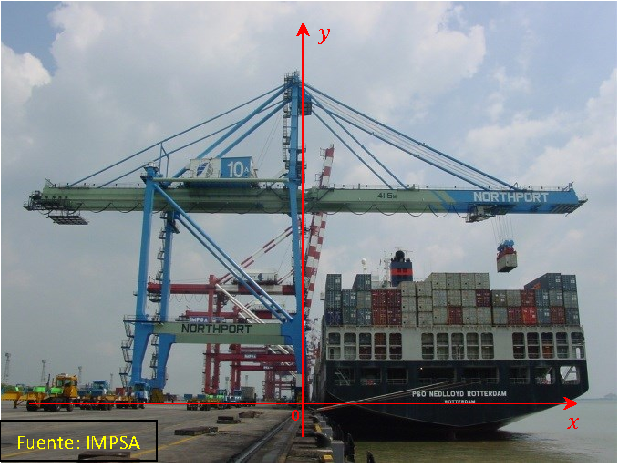
\includegraphics[width=0.64\linewidth]{imagenes_informe/modelo_planta/grua_STS_guia_fig1a.pdf}
\caption{Grúa portacontenedores de muelle tipo STS y movimientos principales de traslación e izaje. Fuente: guía del proyecto [1], figura 1(a); imagen atribuida allí a IMPSA.}
\label{fig:sistema_fisico_STS}
\end{figure}
	
	\par
	\Needspace{5\baselineskip}
	\subsection{Arquitectura jerárquica}
	La arquitectura separa la regulación rápida de las secuencias operativas y las protecciones. La tabla siguiente resume las funciones, los períodos de ejecución y la implementación de cada nivel.
	
	\begin{table}[H]
		\centering
		\caption{Niveles de la arquitectura de control.}
		\begin{tabular}{C{1.5cm} L{4.8cm} C{2.2cm} L{5.5cm}}
			\toprule
			Nivel & Función & Muestreo & Implementación\\
			\midrule
			2 & Control regulatorio de carro e izaje & $1~\mathrm{ms}$ & Bloques discretos de Simulink\\
			1 & Secuencia, referencias, perfil y modos & $20~\mathrm{ms}$ & Stateflow\\
			0 & Seguridad y frenado de emergencia & $20~\mathrm{ms}$ & Stateflow independiente\\
			\bottomrule
		\end{tabular}
	\end{table}
	
\begin{figure}[H]
\centering
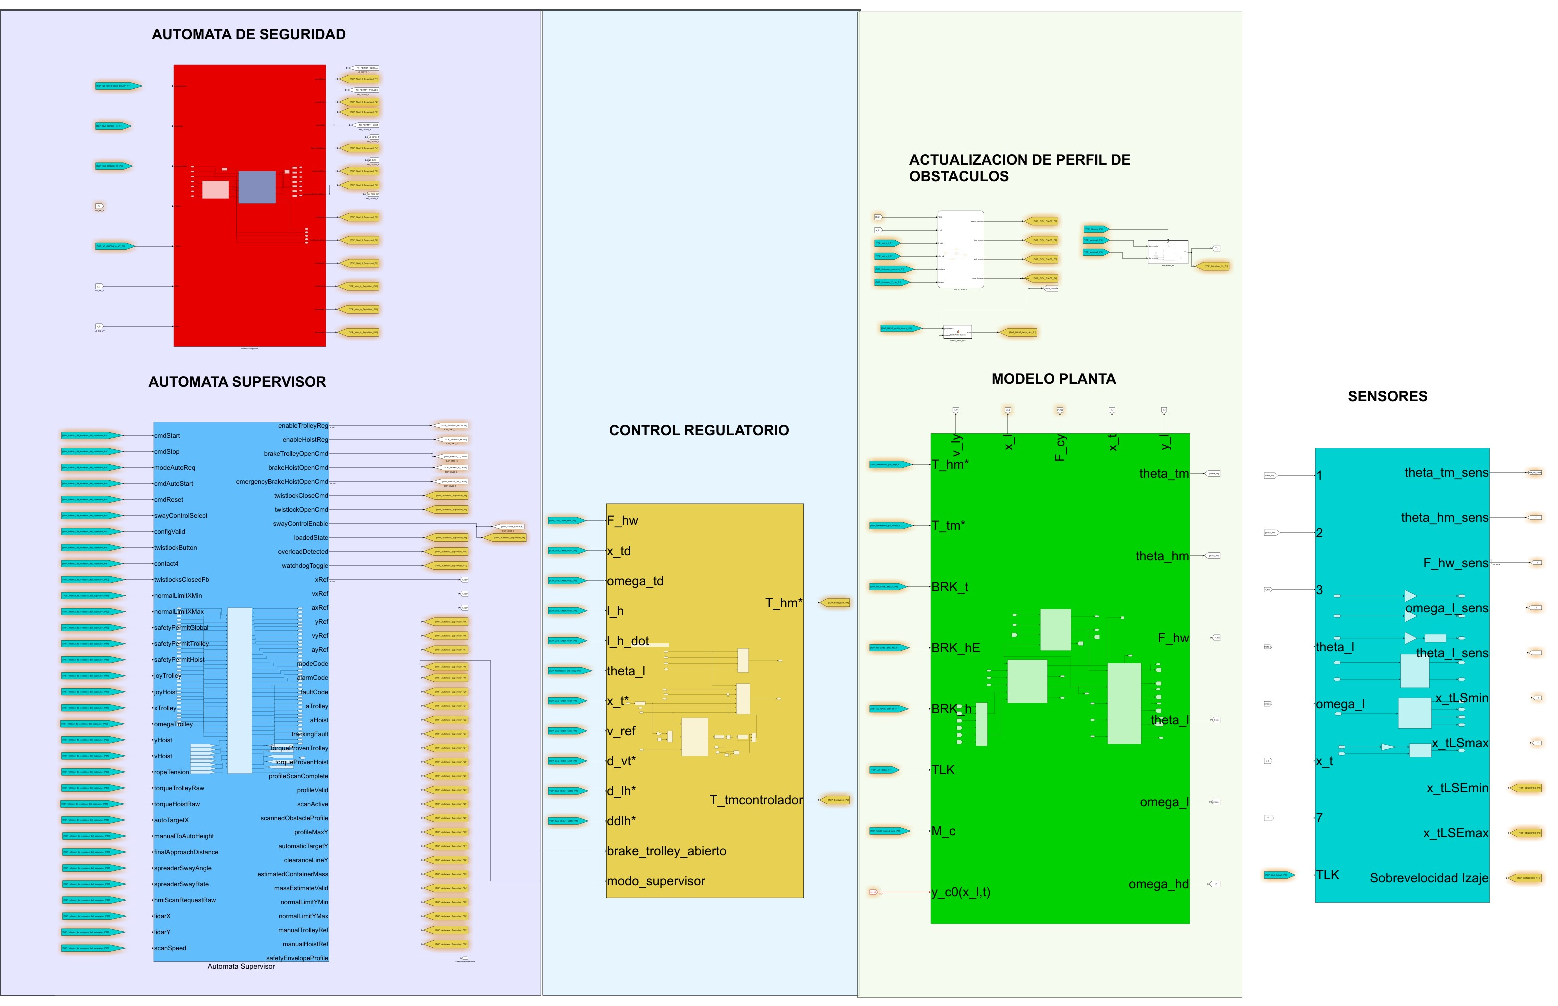
\includegraphics[width=.99\textwidth]{imagenes_informe/arquitectura/sistema_completo_recortado.pdf}
\caption{Implementación del sistema completo en Simulink: autómatas de seguridad y supervisor, control regulatorio, planta, actualización del perfil y sensores.}
\label{fig:sistema_completo}
\end{figure}

	\par
	\Needspace{5\baselineskip}
	\subsection{Variables principales}

Las variables del modelo se agrupan en posiciones y velocidades, longitud y ángulo del cable, fuerzas de tensión y contacto, magnitudes de accionamiento y estados discretos de operación. Sus definiciones y convenciones se establecen en el modelo matemático; el diccionario de señales reúne sus unidades y significado.
\clearpage

\section{Modelo matemático de la planta}
\label{sec:modelo_planta}
	
	\Needspace{5\baselineskip}
	
\subsection{Alcance, hipótesis y coordenadas}
La planta representa, en un plano vertical, el carro, el mecanismo de izaje y el conjunto suspendido formado por el \textit{spreader} y, cuando corresponde, el contenedor. Se adopta $x$ positivo hacia el barco e $y$ positivo hacia arriba. El punto de suspensión está a la altura fija $Y_{t0}=45~\mathrm{m}$; $x_t$ es la posición del carro y $(x_l,y_l)$ la del centro de la base del \textit{spreader}. La longitud geométrica del cable es $l$ y el ángulo de balanceo $\theta_l$ se mide respecto de la vertical.

Como en la guía del proyecto, la estructura se considera rígida, la carga se concentra en un punto y el movimiento se restringe al plano $x$--$y$. Se conservan las no linealidades que modifican el comportamiento durante una maniobra: longitud y ángulo variables, elasticidad unilateral del cable, contacto con el perfil, masa suspendida variable, saturaciones de accionamientos y aplicación de frenos. 
	
	\begin{figure}[H]
\centering
\begingroup
\setlength{\unitlength}{0.98\linewidth}
\begin{picture}(1,0.537)
\put(0,0){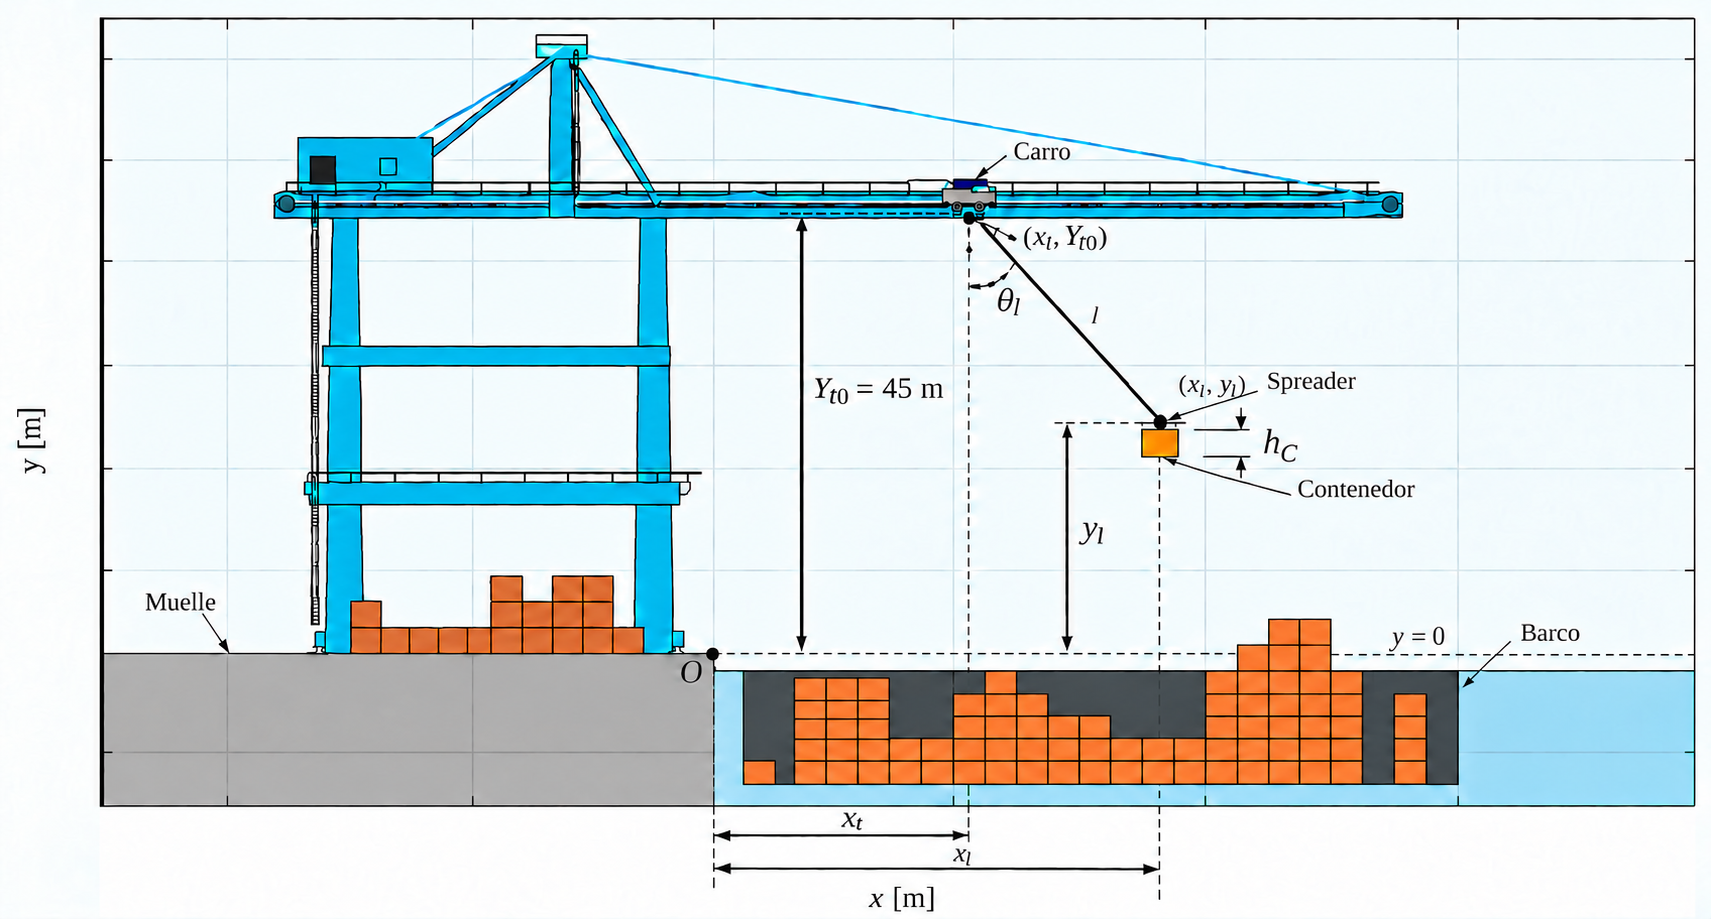
\includegraphics[width=\unitlength]{imagenes_informe/modelo_planta/esquema_planta_visualizacion_v4.png}}
% Rotulación matemática vectorial para conservar el subíndice del carro.
\put(0.596,0.386){\colorbox{white}{\makebox[0.049\linewidth][l]{$\scriptstyle(x_t,Y_{t0})$}}}
\end{picture}
\endgroup
\caption{Geometría y coordenadas del modelo de planta sobre una adaptación de la visualización desarrollada.}
\label{fig:geometria_planta_visualizacion}
\end{figure}
	
\Needspace{5\baselineskip}
	
\subsection{Organización y acoplamiento físico}
En Simulink, \texttt{Planta} reúne tres subsistemas: carga, carro e izaje. El carro entrega $x_t$ y $v_t$ para calcular la geometría del cable; el izaje determina su longitud comandada $l_h$ y la tensión por ramal $F_{hw}$; la tensión actúa simultáneamente sobre la carga y sobre el carro. La carga devuelve su posición, velocidad y ángulo, además de la condición de contacto con el perfil. Por ello los mecanismos no se modelan como movimientos independientes.
	
	\begin{figure}[!htb]
		\centering
		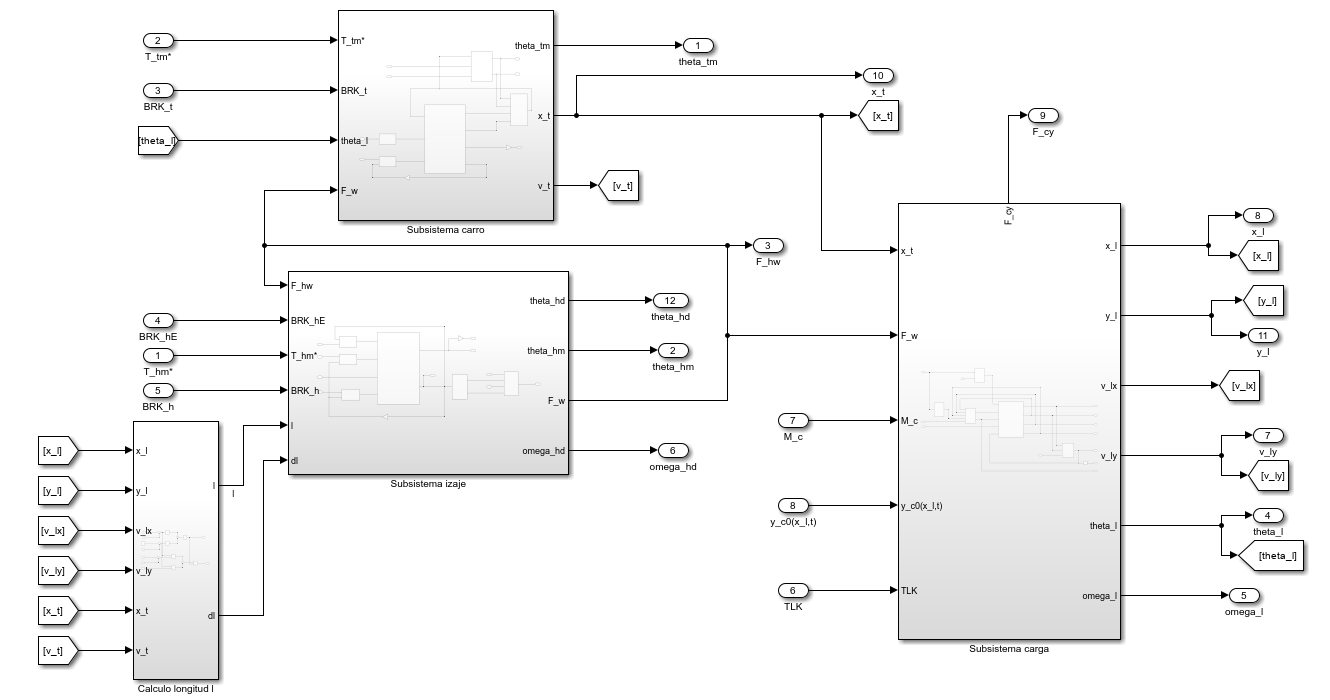
\includegraphics[width=0.95\columnwidth]{imagenes_informe/usuario/P_1.png}
		\caption{Interconexión de los subsistemas de carro, izaje y carga dentro de \texttt{Planta}.}
		\label{fig:planta_general}
	\end{figure}
	
	\Needspace{5\baselineskip}
	
\subsection{Carga suspendida: geometría y masa}
El bloque de geometría obtiene la longitud y el ángulo a partir de las posiciones calculadas por la dinámica:
\begin{align}
		l&=\sqrt{(x_l-x_t)^2+(Y_{t0}-y_l)^2},\label{eq:l}\\
		\dot l&=\frac{(x_l-x_t)(v_{lx}-v_t)-(Y_{t0}-y_l)v_{ly}}{l},\label{eq:ldot}\\
		\theta_l&=\operatorname{atan2}(x_l-x_t,Y_{t0}-y_l).\label{eq:theta}
\end{align}
De forma equivalente, $x_l=x_t+l\sin\theta_l$ e $y_l=Y_{t0}-l\cos\theta_l$. La función de cuatro cuadrantes conserva el signo del balanceo. Las señales $l$ y $\dot l$ alimentan el modelo del cable de izaje; $\theta_l$ determina la dirección de la tensión y se entrega al regulador de balanceo.
	
	\begin{figure}[!htb]
		\centering
		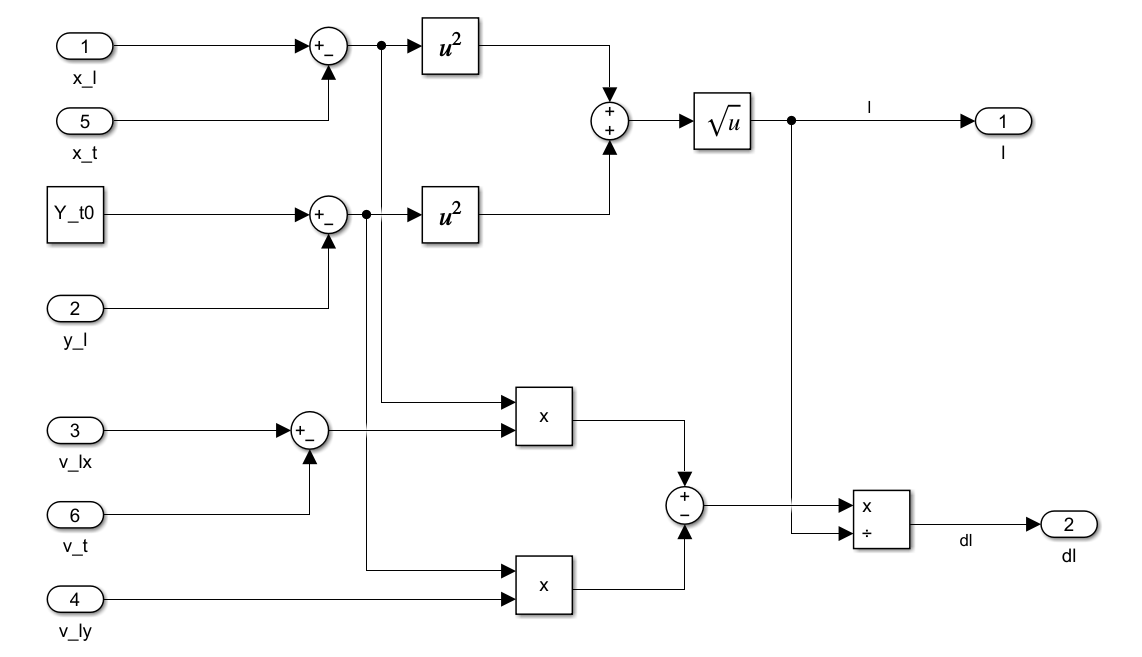
\includegraphics[width=0.88\columnwidth]{imagenes_informe/usuario/P_long1.png}
		\caption{Cálculo de $l$ y $\dot l$ a partir de posiciones y velocidades relativas.}
		\label{fig:longitud_cable}
	\end{figure}
	\begin{figure}[!htb]
		\centering
		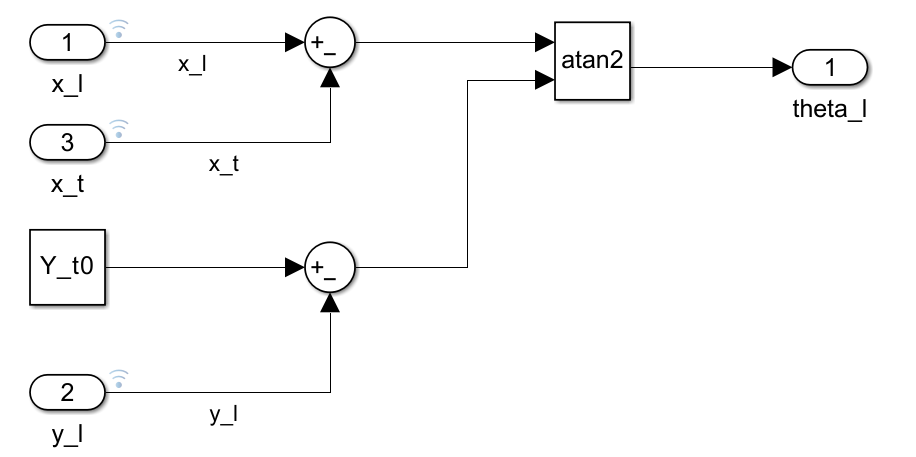
\includegraphics[width=0.75\columnwidth]{imagenes_informe/usuario/P_carga4sw_.png}
		\caption{Cálculo de $\theta_l$ mediante \texttt{atan2} en el subsistema de carga.}
		\label{fig:angulo_carga}
	\end{figure}
	
La masa que interviene en los balances de fuerzas depende de la sujeción del contenedor. Con el \textit{spreader} vacío, $m_l=M_s$ y la altura inferior adicional es $h_c=0$; con el contenedor asegurado, $m_l=M_s+M_c$ y $h_c=H_c$. Se utilizan $M_s=15000~\mathrm{kg}$ y $H_c=2.59~\mathrm{m}$. Esta selección se realiza en el bloque de masa y longitud inferior del subsistema de carga. La estimación de $M_c$ a partir de la tensión, que sirve a la supervisión, se explica junto con esa función de control.
	
	\Needspace{5\baselineskip}
	
\subsection{Carga suspendida: contacto y movimiento}
El perfil $y_{c0}(x_l,t)$ representa la cota de apoyo bajo la carga. La base se encuentra en $y_l-h_c$ y la penetración calculada es $\delta=y_{c0}(x_l,t)-(y_l-h_c)$. Mientras $\delta<0$ no se aplica fuerza de contacto. Para $\delta\geq0$, el bloque utiliza una reacción vertical elástica amortiguada y una fuerza horizontal que se opone al arrastre:
	\begin{align}
		F_{cx}&=-b_{cx}v_{lx},\\
		F_{cy}&=K_{cy}\delta-b_{cy}v_{ly}.
	\end{align}
Se emplean $K_{cy}=1.8\times10^9~\mathrm{N/m}$, $b_{cy}=10\times10^6~\mathrm{N\,s/m}$ y $b_{cx}=1\times10^6~\mathrm{N\,s/m}$. La conmutación por contacto hace que ambas fuerzas sean nulas fuera del apoyo. El perfil que alimenta este bloque y su actualización durante la operación se describen en la \cref{sec:entorno_planta}.
	
	\begin{figure}[!htb]
		\centering
		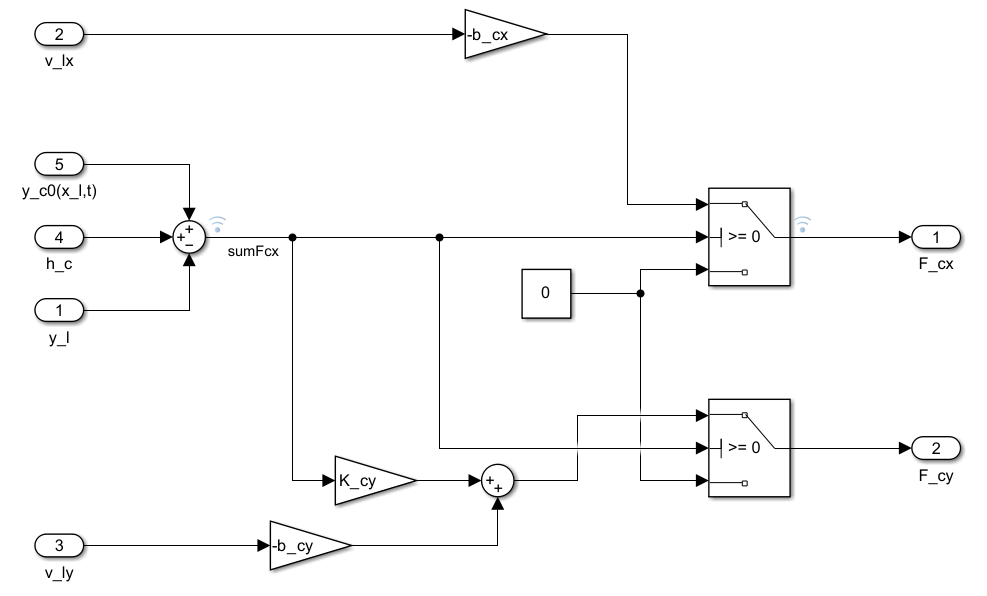
\includegraphics[width=0.86\columnwidth]{imagenes_informe/usuario/P_carga3contacto_.png}
		\caption{Cálculo y conmutación de las fuerzas de contacto a partir de la penetración de la base.}
		\label{fig:contacto_carga}
	\end{figure}
	
	La fuerza del cable se proyecta según el ángulo instantáneo. Los balances que implementa el bloque de movimiento son
	\begin{align}
		m_l\dot v_{lx}&=-2F_{hw}\sin\theta_l+F_{cx},\label{eq:loadx}\\
		m_l\dot v_{ly}&=2F_{hw}\cos\theta_l+F_{cy}-m_lg.\label{eq:loady}
	\end{align}
Dos integraciones sucesivas en cada eje entregan $v_{lx},x_l$ y $v_{ly},y_l$. El factor dos corresponde a los ramales equivalentes de la formulación; $F_{hw}$ es la tensión de uno de ellos. Las posiciones vuelven al cálculo geométrico, cerrando el acoplamiento entre movimiento y tensión.
	
	\begin{figure}[!htb]
		\centering
		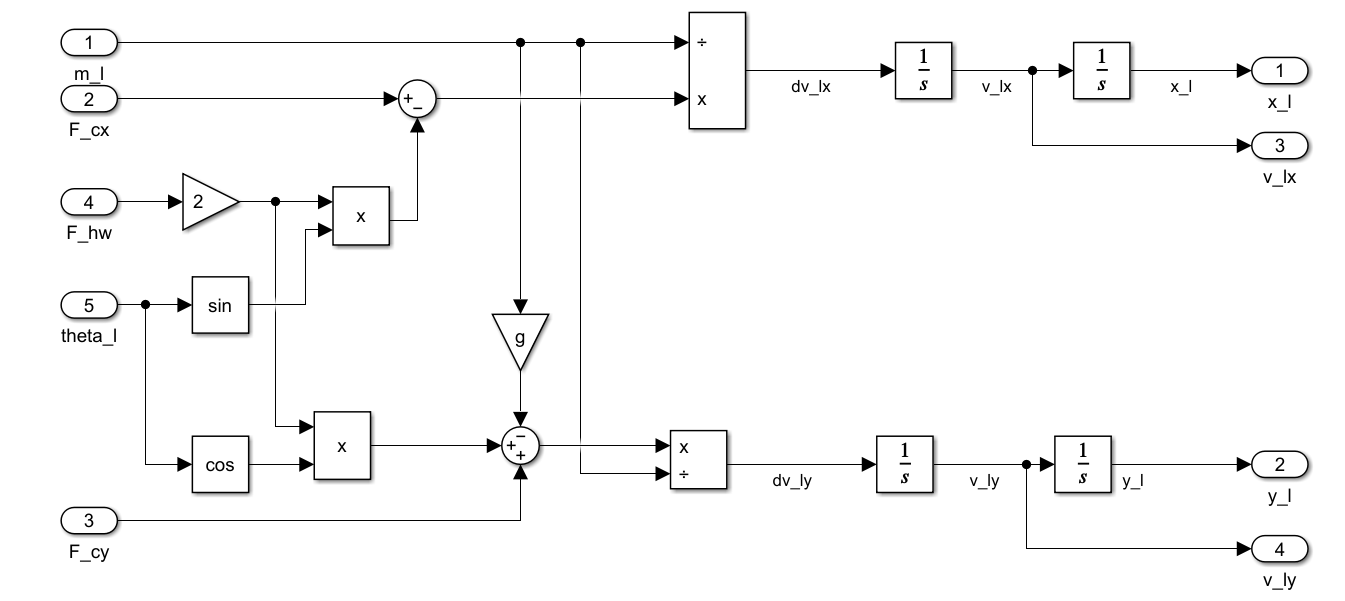
\includegraphics[width=0.94\columnwidth]{imagenes_informe/usuario/P_carga2din_.png}
		\caption{Balances de fuerzas e integradores de velocidad y posición de la carga.}
		\label{fig:dinamica_carga}
	\end{figure}
	
	\Needspace{5\baselineskip}
	
\subsection{Izaje: cable, longitud y tambor}
Se distinguen la longitud geométrica $l$ y la longitud $l_h$ impuesta por el movimiento del tambor. La diferencia entre ambas produce la elongación del cable. Cuando el cable está tenso, la tensión por ramal se calcula como
	\begin{equation}
		F_{hw}=2K_{hw}(l_h)(l-l_h)+2b_{hw}(l_h)(\dot l-\dot l_h),\label{eq:rope}
	\end{equation}
con $K_{hw}(l_h)=k_{hwu}/(2l_h+L_{h0})$ y $b_{hw}(l_h)=b_{hwu}(2l_h+L_{h0})$. En la condición de cable flojo se impone $F_{hw}=0$: el cable transmite tracción, pero no compresión. Los parámetros principales son $k_{hwu}=236\times10^6~\mathrm{N}$, $b_{hwu}=150~\mathrm{N\,s/m^2}$ y $L_{h0}=110~\mathrm{m}$.
	
En equilibrio cuasiestático, la elongación aproximada es
	\begin{equation}
		\Delta l\simeq\frac{m_lg}{4K_{hw}}.\label{eq:stretch}
	\end{equation}
	Esta estimación se usa más adelante al calcular el despeje de la trayectoria.
	
	La relación cinemática $y_h=Y_{t0}-l_h$ implica $v_h=-\dot l_h$. Para el aparejo equivalente, $2v_h=r_{hd}\omega_{hd}$ y el torque resistente en el tambor es $T_{hdl}=F_{hw}r_{hd}$. Esta cadena transforma la rotación del tambor en una variación de longitud y devuelve la tensión como carga mecánica del accionamiento.
	
	\begin{figure}[!htb]
		\centering
		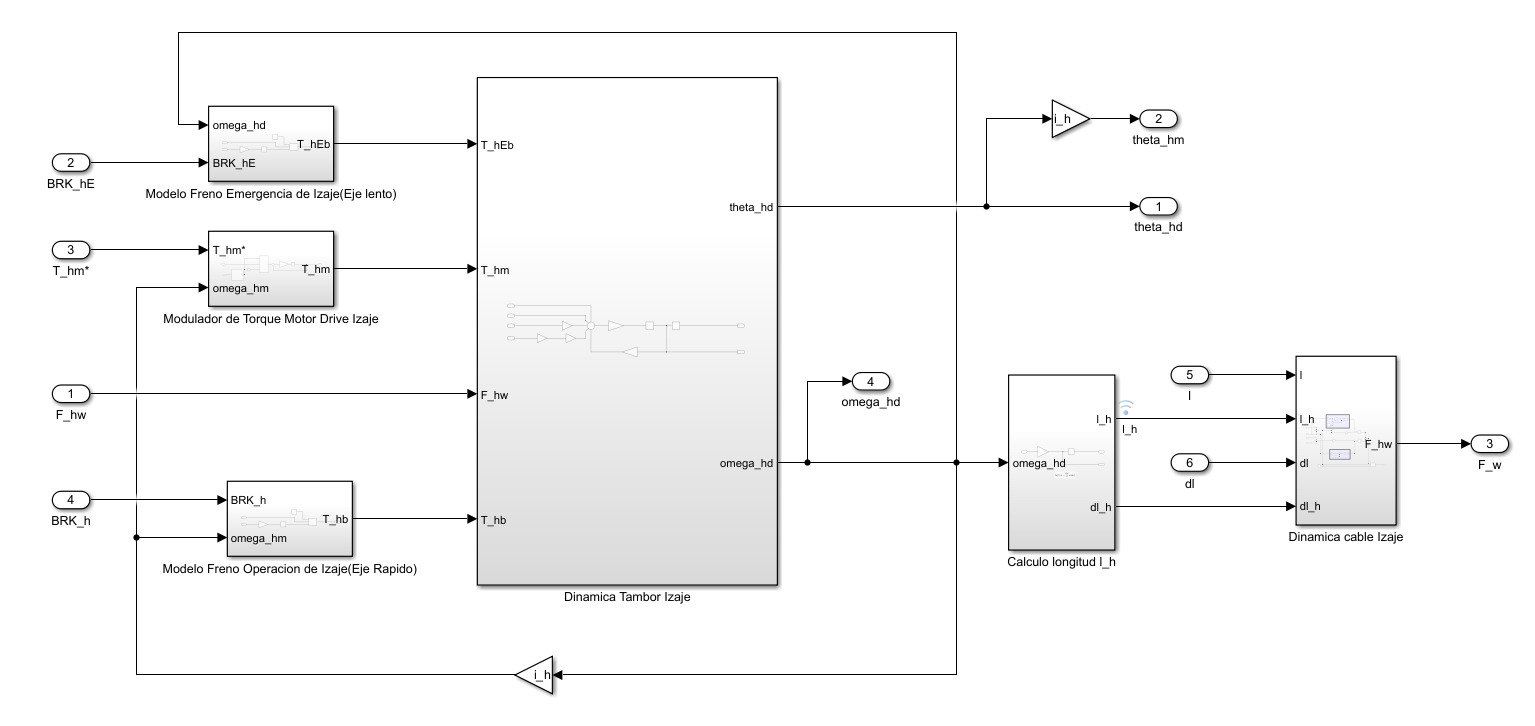
\includegraphics[width=0.94\columnwidth]{imagenes_informe/usuario/P_izj1.png}
		\caption{Cadena de izaje: accionamiento, tambor, longitud comandada y cable elástico.}
		\label{fig:izaje_general}
	\end{figure}
	
	\Needspace{5\baselineskip}
	
	\subsection{Izaje: accionamiento y frenado}
	El subsistema de izaje representa el eje lento del tambor, el reductor y el eje rápido del motor. Sus balances incluyen inercia, rozamiento, torque motor, torque resistente del cable y los torques de freno. La transmisión ideal utiliza $\omega_{hm}=i_h\omega_{hd}$ y $T_{hd}=i_hT_{hml}$, con $i_h=22$. El modulador del motor aproxima la respuesta de torque mediante $\tau_{hm}\dot T_{hm}=T_{hm,\mathrm{lim}}^*-T_{hm}$, con $\tau_{hm}=1~\mathrm{ms}$. La consigna se limita a la capacidad del motor, incluida su reducción a velocidades superiores a la nominal.
	
	El freno de operación actúa en el eje rápido y el de emergencia en el eje lento. Cuando están aplicados generan un torque opuesto a la rotación y limitado en magnitud; cuando están liberados su torque es nulo. Su mando y los enclavamientos para apertura o parada se explican con los autómatas. Aquí interesa que ambos torques entran en el balance mecánico del izaje, como muestra la \cref{fig:izaje_general}. Los valores principales de los accionamientos se reúnen en la \cref{tab:parametros_accionamientos}.
	
	\Needspace{5\baselineskip}
	
	\subsection{Carro: cable, movimiento y accionamiento}
	El tambor del carro fija una posición equivalente $x_{td}$ y una velocidad $v_{td}$. La diferencia con el movimiento real del carro produce la fuerza del cable:
	\begin{equation}
		F_{tw}=K_{tw}(x_{td}-x_t)+b_{tw}(v_{td}-v_t).\label{eq:trolleyrope}
	\end{equation}
	El balance traslacional, con $\dot x_t=v_t$, es
	\begin{equation}
		M_t\dot v_t=F_{tw}-b_tv_t+2F_{hw}\sin\theta_l.\label{eq:trolley}
	\end{equation}
	El último término es la reacción horizontal de la carga suspendida sobre el carro. Se utilizan $M_t=30000~\mathrm{kg}$, $K_{tw}=480~\mathrm{kN/m}$, $b_{tw}=3~\mathrm{kN\,s/m}$ y $b_t=90~\mathrm{N\,s/m}$.
	
	El accionamiento transforma $\omega_{td}$ en $v_{td}=r_{td}\omega_{td}$, con $r_{td}=0.5~\mathrm{m}$, y refleja la fuerza del cable como torque resistente $T_{tdl}=F_{tw}r_{td}$. El reductor ideal relaciona $\omega_{tm}=i_t\omega_{td}$, con $i_t=30$. El motor recibe el torque limitado del modulador y el torque del freno de operación. El modelo conserva las inercias y pérdidas de tambor y motor como estados mecánicos, en lugar de reemplazarlas por una sola ganancia.
	
	\begin{figure}[!htb]
		\centering
		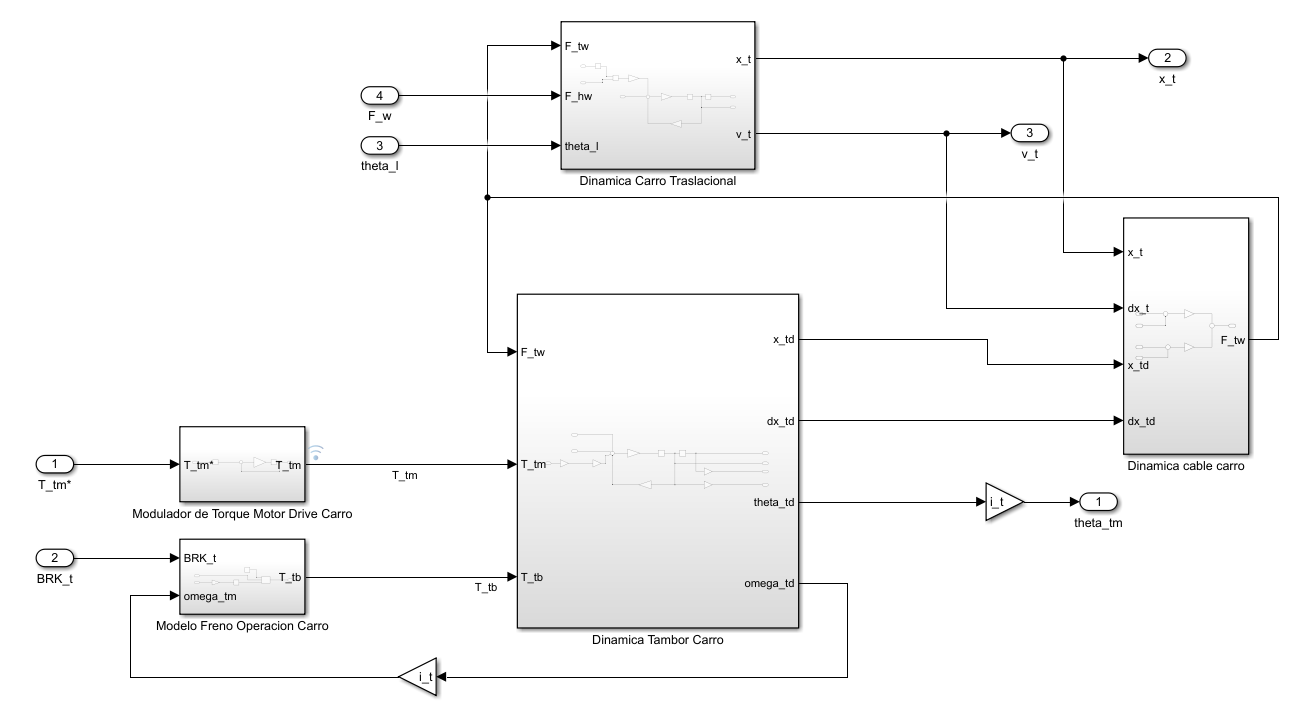
\includegraphics[width=0.94\columnwidth]{imagenes_informe/usuario/P_carro1.png}
		\caption{Cadena del carro: torque, tambor, cable elástico y movimiento traslacional.}
		\label{fig:carro_general}
	\end{figure}
	
	\begin{table}[!htb]
		\centering
		\caption{Parámetros principales de los accionamientos de la planta.}
		\begin{tabular}{L{5.6cm} C{3.0cm} C{3.5cm}}
			\toprule
			Magnitud & Carro & Izaje\\
			\midrule
			Radio de tambor & $0.5~\mathrm{m}$ & $0.75~\mathrm{m}$\\
			Relación de transmisión & $30$ & $22$\\
			Constante de tiempo del modulador & $1~\mathrm{ms}$ & $1~\mathrm{ms}$\\
			Límite nominal de torque motor & $4~\mathrm{kN\,m}$ & $20~\mathrm{kN\,m}$\\
			Torque máximo del freno de operación & $5~\mathrm{kN\,m}$ & $50~\mathrm{kN\,m}$\\
			Torque máximo del freno de emergencia & --- & $1.1~\mathrm{MN\,m}$\\
			\bottomrule
		\end{tabular}
		\label{tab:parametros_accionamientos}
	\end{table}

\par
\Needspace{10\baselineskip}
\section{Implementación en MATLAB y Simulink}
\label{sec:implementacion_planta}
	
	\Needspace{5\baselineskip}
	
	\subsection{Archivo de modelo e inicialización}
	La implementación de referencia es \path{Modelo_Final_24092026_2024a.slx}, dentro del paquete \path{SEPTIEMBRE/Modelo_Final_24092026/Paquete_Modelo_Final_HMI_Corregido_Ordenado}. El archivo \path{parametros_ganancias_cascada_29072026.m} reúne constantes físicas, límites, condiciones iniciales y ganancias. En el informe se separarán conceptualmente los parámetros de planta de las ganancias de control, aunque compartan el archivo de inicialización. Antes de la entrega se comprobará que esta denominación coincide con la versión finalmente utilizada para las pruebas.
	
	\Needspace{5\baselineskip}
	
	\subsection{Jerarquía de subsistemas y flujo de señales}

La implementación conserva la división de la planta en carga, carro e izaje presentada en el modelo matemático. Los bloques dinámicos integran las velocidades y posiciones, mientras que las relaciones geométricas y las fuerzas se calculan algebraicamente. Los cambios de masa, contacto, tensión y frenado seleccionan el comportamiento correspondiente dentro de esta estructura.
\Needspace{5\baselineskip}

\subsection{Sensores y señales disponibles para el control}
	La planta entrega magnitudes físicas; el subsistema \texttt{SENSORES} representa las mediciones y detecciones que utiliza el control. Los encoders del carro y del izaje toman las posiciones angulares de sus motores, $\theta_{tm}$ y $\theta_{hm}$. En esta versión tienen ganancia unitaria, de modo que sus salidas reproducen esas posiciones sin cuantización ni ruido añadidos. El ángulo de la carga y su velocidad angular también se transmiten sin una dinámica de medición adicional.
	
	La tensión del cable se trata de manera distinta. La celda de carga conserva la escala de $F_{hw}$ y pasa la señal por un filtro de primer orden, $G_F(s)=1/(0.1s+1)$. Así, $F_{hw,\mathrm{sens}}$ responde con un retardo de medición respecto de la tensión física utilizada en la planta. Esta diferencia importa para las condiciones de detección basadas en tensión y para la estimación de masa.
	
	El mismo subsistema genera señales discretas a partir de variables continuas. Los finales de carrera del carro comparan $x_t$ con los límites de operación y de emergencia de ambos extremos. El detector de sobrevelocidad de izaje utiliza la velocidad obtenida del tambor y el estado de los \textit{twistlocks}, para aplicar el umbral correspondiente a la condición cargada o vacía; la captura lo identifica como el 115\,\% del límite nominal. Estas señales se entregan a los autómatas. Su lógica de respuesta se presenta en las secciones de supervisor y seguridad.
	
	\begin{figure}[!htb]
		\centering
		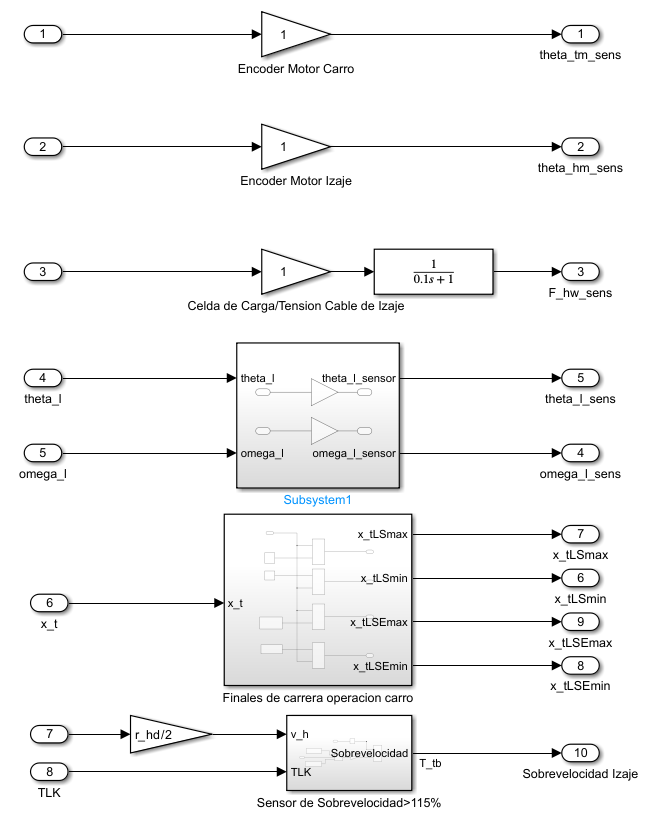
\includegraphics[width=0.78\columnwidth]{imagenes_informe/usuario/Sens_1.png}
		\caption{Señales de medición y detecciones disponibles para el control.}
		\label{fig:sensores_planta}
	\end{figure}
	
	\Needspace{5\baselineskip}
	
	\subsection{Perfil de obstáculos y LIDAR simulado}
	\label{sec:entorno_planta}
	El entorno conserva una altura de base $Z_{\mathrm{base}}(k)$ y un número de contenedores $n_k$ por cada posición discreta o \textit{slot} $k$. El ancho de un \textit{slot} es $W_c=2.44~\mathrm{m}$ y su cota se obtiene como
	\begin{equation}
		Y_c(k)=Z_{\mathrm{base}}(k)+n_kH_c.
		\label{eq:perfil_slots}
	\end{equation}
	Una consulta espacial de este vector proporciona $y_{c0}(x_l,t)$ al bloque de contacto de la carga. Por ello, al modificar $n_k$, también cambia la superficie física con la que puede entrar en contacto el contenedor.
	
	El LIDAR se simula consultando el perfil a partir de la posición del sensor. En la orientación utilizada, está $3~\mathrm{m}$ por delante del carro:
	\begin{equation}
		x_{\mathrm{LIDAR}}=x_t+3~\mathrm{m}.
	\end{equation}
	La tabla devuelve la cota asociada a esa posición y entrega las muestras de posición y altura al supervisor. El movimiento de barrido y los criterios para validar el perfil relevado se describirán con el autómata supervisor.
	
	\Needspace{5\baselineskip}
	
	\subsection{Reconocimiento de toma y depósito}
	La actualización del perfil necesita saber cuándo un contenedor fue realmente retirado o depositado. Para ello, el \textit{statechart} \texttt{PICK / PLACE} combina posición válida de \textit{slot}, contacto, tensión, estado de los \textit{twistlocks} y velocidad vertical. Sus estados \texttt{VACIO1} y \texttt{CARGADO1} indican si la carga está asociada al \textit{spreader}; \texttt{PRE\_PICK} y \texttt{PRE\_PLACE} conservan la información necesaria mientras se completa una toma o un depósito.
	
	Desde \texttt{VACIO1}, el contacto con un \textit{slot} válido y los \textit{twistlocks} abiertos llevan a \texttt{PRE\_PICK}; allí se memoriza el índice del \textit{slot}. Solo cuando los \textit{twistlocks} están cerrados, hay tensión, se pierde el contacto y el conjunto asciende por encima del umbral de velocidad se confirma la toma. La transición emite \texttt{evento\_cambio}, \texttt{tipo\_evento=1} y el índice memorizado, y pasa a \texttt{CARGADO1}. Si desaparecen las condiciones de preparación, se descarta el índice y se vuelve a vacío.
	
	Desde \texttt{CARGADO1}, el contacto con un \textit{slot} válido y la velocidad vertical próxima a cero llevan a \texttt{PRE\_PLACE}; también aquí se memoriza el lugar de apoyo. El depósito se confirma cuando se abren los \textit{twistlocks} y persiste el contacto. Se emite un único evento de tipo $2$ para ese \textit{slot} y se vuelve a \texttt{VACIO1}. Las señales de contacto y tensión se acondicionan con histéresis antes de entrar al \textit{statechart}, evitando oscilaciones de estado cerca de los umbrales. Las velocidades exigidas en las transiciones ayudan a distinguir una maniobra efectiva de un contacto momentáneo.
	
	\begin{figure}[!htb]
		\centering
		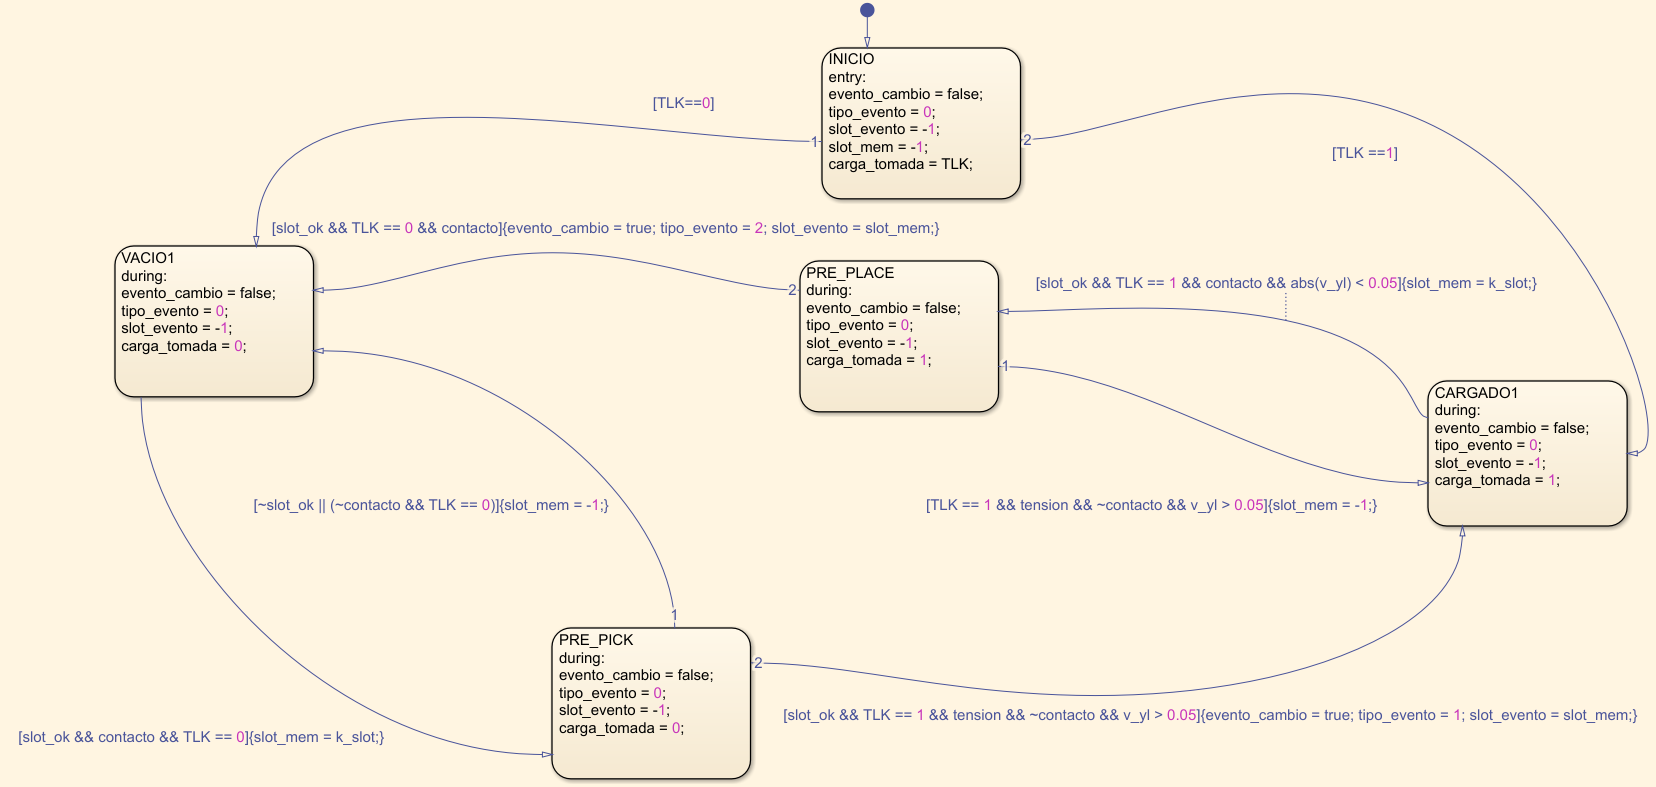
\includegraphics[width=0.98\columnwidth]{imagenes_informe/usuario/PickPlace_chart.png}
		\caption{Estados y condiciones de confirmación de toma y depósito en \texttt{PICK / PLACE}.}
		\label{fig:pick_place_chart}
	\end{figure}
	
	\Needspace{5\baselineskip}
	
	\subsection{Actualización del perfil}
	Las salidas del \textit{statechart} atraviesan memorias antes de entrar a \texttt{Actualizar\_Yc}. El pulso \texttt{evento\_cambio} habilita el cambio; \texttt{tipo\_evento} indica si se retira o deposita un contenedor y \texttt{slot\_evento} identifica dónde ocurrió. El perfil actualizado alimenta la tabla espacial que entrega la altura bajo $x_l$ y retorna a la dinámica de contacto.
	
	\begin{figure}[!htb]
		\centering
		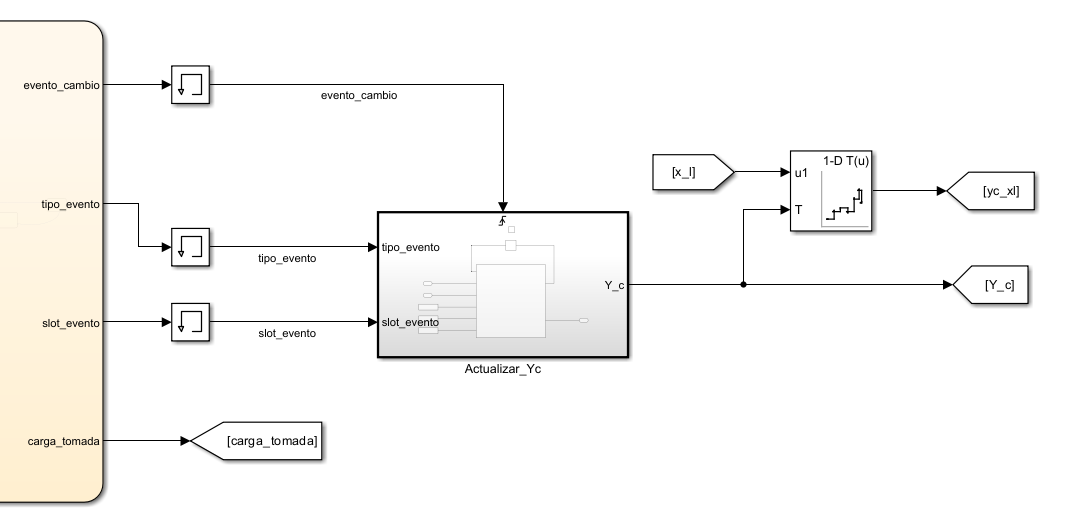
\includegraphics[width=0.91\columnwidth]{imagenes_informe/usuario/PickPlace_actObs.png}
		\caption{Conexión entre el evento de \texttt{PICK / PLACE}, la actualización del perfil y su consulta espacial.}
		\label{fig:actualizar_perfil_bloques}
	\end{figure}
	
	La función \texttt{update\_profile\_std} actualiza el número de contenedores del slot indicado por cada evento de toma o depósito y recalcula su cota. La operación se realiza únicamente sobre slots válidos y no bloqueados, evitando cantidades negativas de contenedores. El perfil actualizado alimenta la consulta espacial utilizada por el modelo de contacto.
	
	\Needspace{22\baselineskip}
\begin{samepage}
\begin{lstlisting}[language=Matlab,caption={Actualización del perfil de contenedores por evento.},label={lst:update_profile_std}]
		function [nLevels_new, Y_c] = update_profile_std( ...
		nLevels, tipo_evento, slot_evento, ...
		Zbase, slotBlock, h_std)
		Nslots = int32(length(nLevels));
		nLevels_new = nLevels;
		slot = int32(slot_evento);
		slot_ok = (slot >= 1) && (slot <= Nslots) && (~slotBlock(slot));
		
		if slot_ok
		if tipo_evento == 1
		nLevels_new(slot) = max(nLevels_new(slot) - 1, 0);
		elseif tipo_evento == 2
		nLevels_new(slot) = nLevels_new(slot) + 1;
		end
		end
		
		Y_c = Zbase + double(nLevels_new) * h_std;
		Y_c(slotBlock) = Zbase(slotBlock);
		end
	\end{lstlisting}
\end{samepage}
	
	\par
	\Needspace{5\baselineskip}
	\subsection{Configuración temporal}
	La planta mecánica y los moduladores se representan con dinámica continua. El control regulatorio entrega consignas muestreadas cada $T_s=1~\mathrm{ms}$; supervisor y seguridad ejecutan su lógica cada $20~\mathrm{ms}$. Las fronteras entre estos ritmos emplean retenciones y memorias según la señal. Esta distinción permite interpretar correctamente una orden discreta de freno o cambio de carga aplicada a un modelo físico continuo.

\par
\Needspace{10\baselineskip}
\section{Control regulatorio}
\Needspace{5\baselineskip}
\subsection{Estructura general}
	El sistema controlado comprende el carro, el izaje y la carga suspendida. Es subactuado respecto del balanceo: no hay un actuador que aplique directamente un par a la carga, por lo que la oscilación se atenúa mediante el movimiento del carro. El izaje también influye en la dinámica pendular, ya que modifica la longitud del cable y, en consecuencia, su período natural.
	Para el carro se implementó una estructura de control en cascada. El lazo exterior corrige la referencia de velocidad a partir del error de posición, mientras que el lazo interior PI calcula la aceleración comandada. A partir de esta aceleración, un bloque de compensación dinámica estima el torque necesario para el accionamiento. La acción anti-sway modifica la referencia de velocidad según el error entre el ángulo medido y su referencia, que puede variar durante la aceleración y el frenado. Para el izaje se empleó un controlador PID sobre la longitud del cable, acompañado por una compensación de tensión. Ambos controladores reciben referencias de posición, velocidad y aceleración generadas por el nivel supervisor.
	
La figura~\ref{fig:cr-sistema} muestra las señales que ingresan al nivel regulatorio y su interfaz de muestreo. La figura~\ref{fig:cr-general} presenta la distribución interna de las funciones de control.

\begin{figure}[H]
\centering
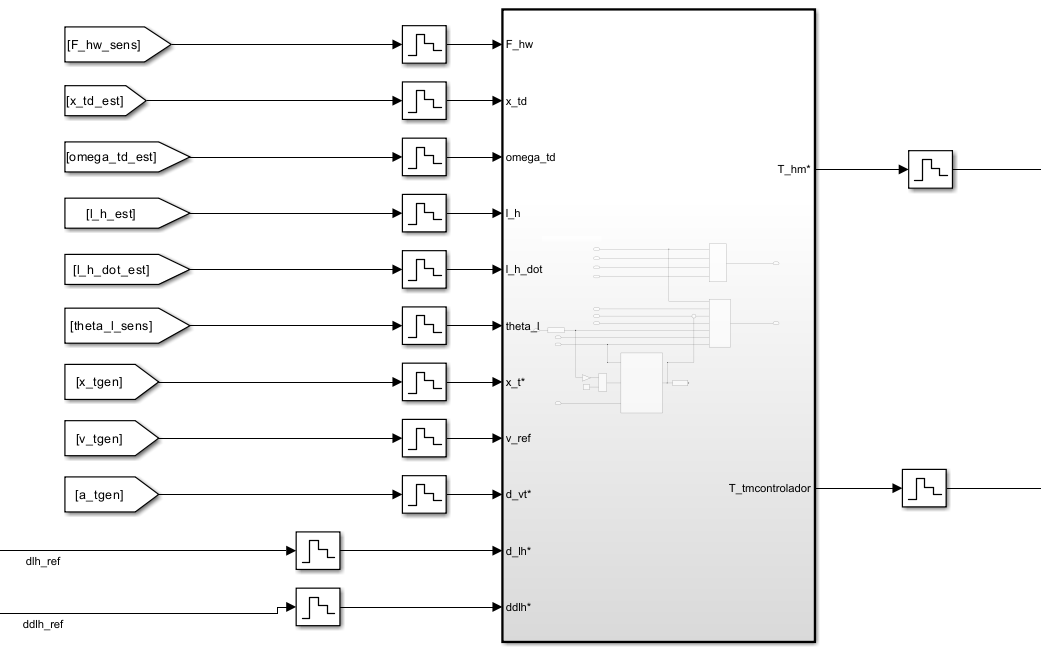
\includegraphics[width=0.90\linewidth]{imagenes_informe/usuario/CR_sist0.png}
\caption{Interfaz del control regulatorio con las mediciones, las referencias y los bloques de muestreo.}
\label{fig:cr-sistema}
\end{figure}

\begin{figure}[H]
\centering
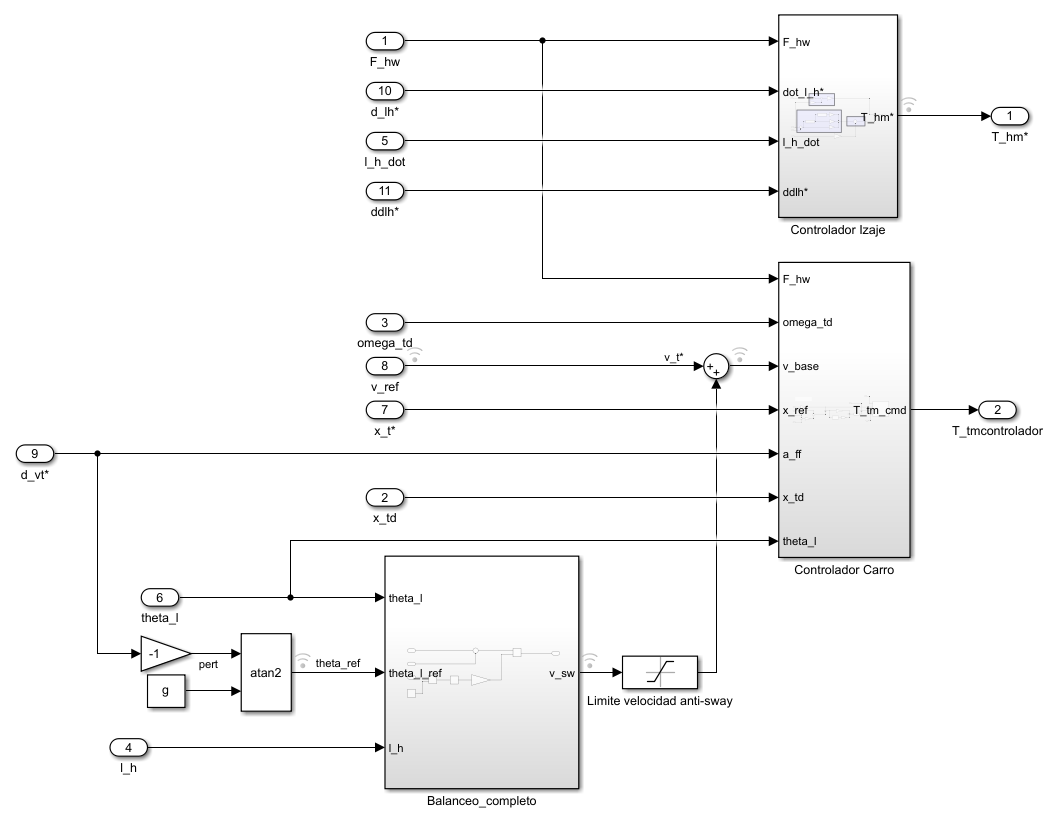
\includegraphics[width=0.88\linewidth]{imagenes_informe/usuario/CR_gral1.png}
\caption{Estructura interna del control regulatorio: carro, izaje, referencia angular y corrección anti-sway.}
\label{fig:cr-general}
\end{figure}
	
	
	\Needspace{5\baselineskip}
	
	
	\subsection{Observadores continuos de velocidad y conversiones cinemáticas}
\label{sec:observadores-continuos}

Los reguladores del carro y del izaje requieren señales de posición y velocidad de sus respectivos accionamientos. Los encoders proporcionan las posiciones angulares de los motores, $\theta_{tm}$ y $\theta_{hm}$. Las posiciones cinemáticas se obtienen mediante las relaciones de transmisión y la geometría de los tambores. Para reconstruir las velocidades se utilizan dos observadores continuos independientes, uno por eje, con la misma estructura y los mismos parámetros de diseño.


\subsubsection{Modelo cinemático y observabilidad}

Para formular el observador se consideran el ángulo del tambor $q$ y su velocidad angular $\omega$. El modelo cinemático adoptado es:
\begin{equation}
\dot q=\omega,\qquad \dot\omega=0.
\end{equation}
La segunda ecuación constituye la hipótesis de predicción del observador. El accionamiento real puede acelerar y frenar; esos cambios se reflejan en la evolución de la medición y producen correcciones sobre los estados estimados.

La lectura angular del motor se convierte en ángulo de tambor mediante:
\begin{equation}
u=\frac{\theta_{m,\mathrm{sens}}}{i},
\end{equation}
donde $i$ es la relación de transmisión. En este apartado, $u$ representa la medición que ingresa al observador. Para una medición ideal, $u=q$.

Definiendo el vector de estados:
\begin{equation}
\boldsymbol x=\begin{bmatrix}q\\\omega\end{bmatrix},
\end{equation}
el modelo se expresa como:
\begin{equation}
\dot{\boldsymbol x}=A_0\boldsymbol x,\qquad u=C\boldsymbol x,
\end{equation}
con:
\begin{equation}
A_0=\begin{bmatrix}0&1\\0&0\end{bmatrix},\qquad
C=\begin{bmatrix}1&0\end{bmatrix}.
\end{equation}
La matriz de observabilidad resulta:
\begin{equation}
\mathcal O=\begin{bmatrix}C\\CA_0\end{bmatrix}
=\begin{bmatrix}1&0\\0&1\end{bmatrix}.
\end{equation}
Luego el modelo es observable bajo la hipótesis cinemática adoptada, y la evolución temporal del ángulo medido permite reconstruir la velocidad angular.

\subsubsection{Formulación del observador}

Se adopta un observador de Luenberger de la forma:
\begin{equation}
\dot{\hat{\boldsymbol x}}=A_0\hat{\boldsymbol x}
+L\left(u-C\hat{\boldsymbol x}\right),
\end{equation}
donde:
\begin{equation}
\hat{\boldsymbol x}=\begin{bmatrix}\hat q\\\hat\omega\end{bmatrix},\qquad
L=\begin{bmatrix}l_1\\l_2\end{bmatrix}.
\end{equation}
Al desarrollar sus componentes se obtiene:
\begin{equation}
\boxed{\dot{\hat q}=\hat\omega+l_1(u-\hat q)},\qquad
\boxed{\dot{\hat\omega}=l_2(u-\hat q)}.
\label{eq:observador-continuo}
\end{equation}
La diferencia $u-\hat q$ es el error entre el ángulo medido y el estimado. Este error corrige la evolución del estado angular interno y de la velocidad estimada.

El estado $\hat q$ se utiliza internamente para generar dicha corrección. Las posiciones empleadas por los reguladores se calculan directamente desde los encoders.

\subsubsection{Asignación de polos y parámetros}

En ausencia de ruido y cuando el movimiento satisface el modelo de velocidad constante, el error de estimación:
\begin{equation}
\boldsymbol e=\boldsymbol x-\hat{\boldsymbol x}
\end{equation}
evoluciona según:
\begin{equation}
\dot{\boldsymbol e}=(A_0-LC)\boldsymbol e =
\begin{bmatrix}-l_1&1\\-l_2&0\end{bmatrix} \boldsymbol e
\end{equation}
cuyo polinomio característico resulta:
\begin{equation}
P_o(s)=\det(sI-A_o)=s^2+l_1s+l_2.
\end{equation}
Se asigna un comportamiento de segundo orden mediante:
\begin{equation}
P_o(s)=s^2+2\zeta_o\omega_os+\omega_o^2.
\end{equation}
Por comparación de coeficientes:
\begin{equation}
\boxed{l_1=2\zeta_o\omega_o,\qquad l_2=\omega_o^2}.
\end{equation}
En ambos ejes se utilizan:
\begin{equation}
\zeta_o=1,\qquad \omega_o=40\ \mathrm{rad/s},
\end{equation}
por lo que:
\begin{equation}
l_1=80\ \mathrm{s^{-1}},\qquad l_2=1600\ \mathrm{s^{-2}}.
\end{equation}
De modo que los dos polos se ubican en:
\begin{equation}
\boxed{p_{o1}=p_{o2}=-40\ \mathrm{s^{-1}}},
\end{equation}
correspondientes a un diseño críticamente amortiguado. La escala temporal asociada es $1/\omega_o=0{,}025\ \mathrm{s}$.

\subsubsection{Interpretación como derivada filtrada}

Aplicando la transformada de Laplace con condiciones iniciales nulas:
\begin{align}
s\hat Q(s)&=\hat\Omega(s)+l_1\left[U(s)-\hat Q(s)\right],\\
s\hat\Omega(s)&=l_2\left[U(s)-\hat Q(s)\right].
\end{align}
Eliminando el estado angular interno se obtiene:
\begin{equation}
\frac{\hat\Omega(s)}{U(s)}=
\frac{\omega_o^2s}{s^2+2\zeta_o\omega_os+\omega_o^2}.
\end{equation}
Por tanto, el observador equivale a una derivada acompañada por un filtro de segundo orden. Para los parámetros seleccionados:
\begin{equation}
\frac{\hat\Omega(s)}{U(s)}=s\,\frac{1600}{(s+40)^2}.
\end{equation}
A frecuencias suficientemente menores que $\omega_o$, la transferencia aproxima al operador derivada. A altas frecuencias su magnitud decrece, limitando la amplificación que produciría una derivación ideal sobre las perturbaciones de la medición.

Para una medición ideal, la relación entre la velocidad estimada y la real, con condiciones iniciales nulas, es:
\begin{equation}
\boxed{\frac{\hat\Omega(s)}{\Omega(s)}=
\frac{\omega_o^2}{s^2+2\zeta_o\omega_os+\omega_o^2}}.
\end{equation}


\subsubsection{Error de estimación durante aceleraciones}

Para una medición ideal, se definen los errores entre las variables reales y las estimadas:
\begin{equation}
e_q=q-\hat q,\qquad e_\omega=\omega-\hat\omega,
\end{equation}
Considerando que la aceleración angular del tambor es \(\dot\omega=a_\theta\), la dinámica del error resulta:
\begin{equation}
\boxed{\dot e_q=e_\omega-l_1e_q},\qquad
\boxed{\dot e_\omega=a_\theta-l_2e_q}.
\end{equation}
Los polos asignados garantizan que, a velocidad constante, los errores converjan a cero. Durante las aceleraciones, \(a_\theta\) actúa como una entrada sobre esta dinámica y puede mantener un error de seguimiento.

Ante una aceleración constante sostenida, una vez extinguido el transitorio:

\begin{equation}
e_q=\frac{a_\theta}{\omega_o^2},\qquad
e_\omega=\frac{2\zeta_o}{\omega_o}a_\theta.
\end{equation}
Con los parámetros adoptados:
\begin{equation}
\boxed{e_\omega=(0{,}05\ \mathrm{s})\,a_\theta}.
\end{equation}

Cuando la aceleración cesa, el error decae a cero. Aumentar \(\omega_o\) reduce este error de seguimiento, aunque también aumenta la sensibilidad a las variaciones rápidas y al ruido de la medición.


\subsubsection{Conversiones cinemáticas y alcance de las estimaciones}

Para el carro, la lectura reducida del encoder y la velocidad angular estimada se convierten mediante:
\begin{equation}
u_t=\frac{\theta_{tm,\mathrm{sens}}}{i_t},\qquad
x_{td,\mathrm{enc}}=r_{td}u_t,\qquad
\hat v_{td}=r_{td}\hat\omega_{td}.
\end{equation}

Para el izaje:
\begin{equation}
u_h=\frac{\theta_{hm,\mathrm{sens}}}{i_h},\qquad
{l_h=l_0-\frac{r_{hd}}2u_h},\qquad
\widehat{\dot l_h}=-\frac{r_{hd}}2\hat\omega_{hd}.
\end{equation}

El funcionamiento de los observadores continuos se verificó reproduciendo las señales de los encoders registradas durante una maniobra con movimiento de ambos ejes y comparando las velocidades estimadas con las correspondientes variables de los accionamientos de la planta simulada. Se obtuvo un buen seguimiento, con errores RMS de \(0{,}00540\ \mathrm{m/s}\) para el carro y \(0{,}00682\ \mathrm{m/s}\) para el izaje, y errores máximos absolutos de \(0{,}02957\ \mathrm{m/s}\) y \(0{,}10548\ \mathrm{m/s}\), respectivamente. Las diferencias se concentraron en los transitorios rápidos y fueron consistentes con el retraso de seguimiento propio del filtrado.


La \cref{fig:observadores-continuos-bloques} muestra la realización de ambos observadores y las conversiones cinemáticas empleadas por los reguladores.

\begin{figure}[H]
\centering
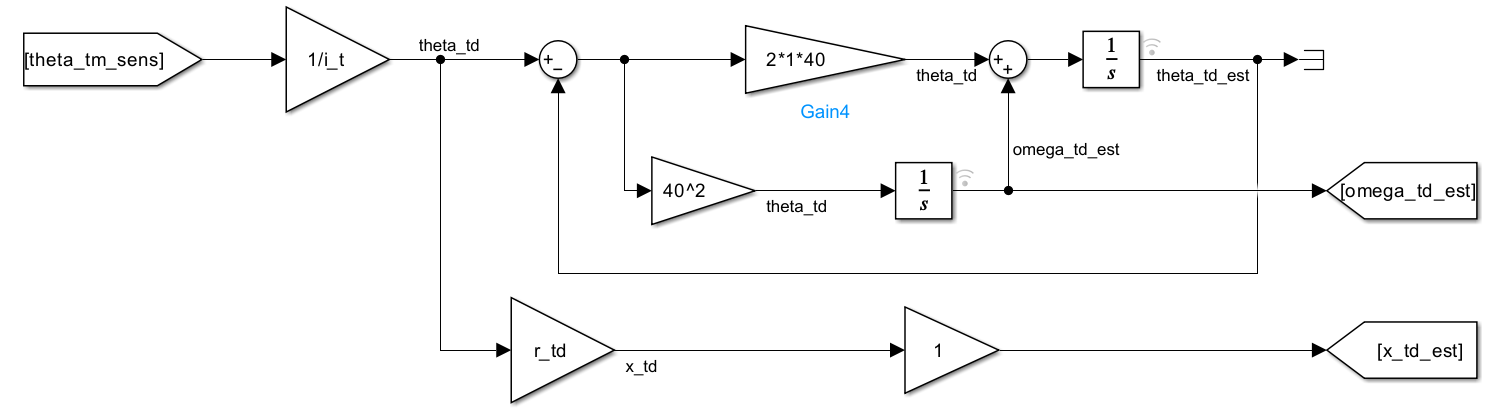
\includegraphics[width=\linewidth]{imagenes_informe/usuario/observador_continuo_carro.png}
\par\vspace{1mm}
{\small (a) Observador del accionamiento del carro y conversión de posición.}
\par\vspace{4mm}
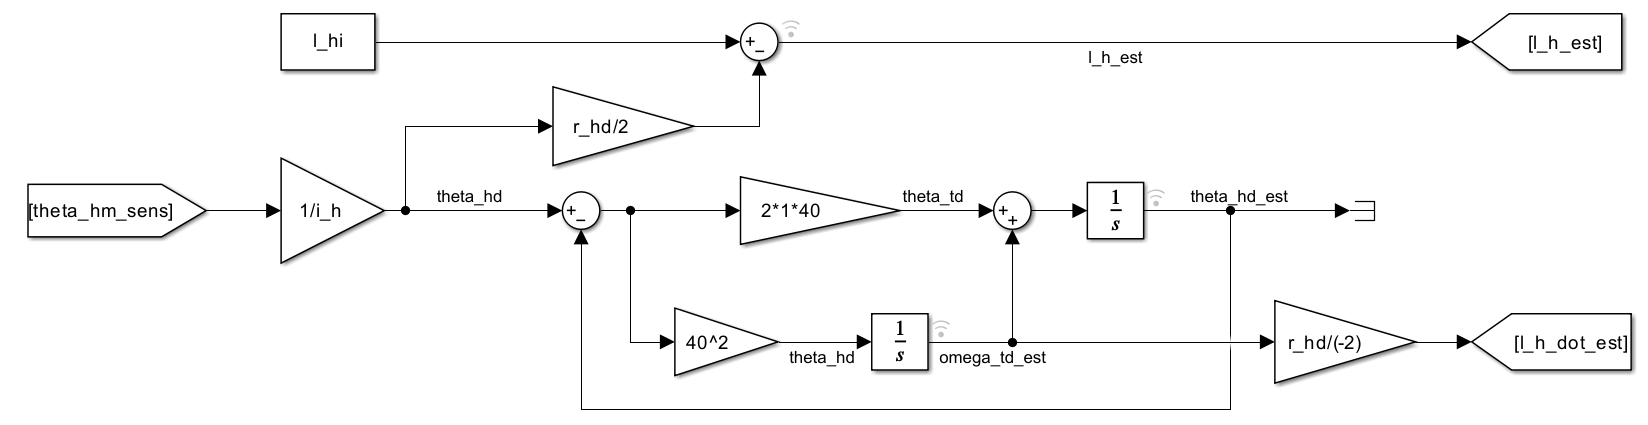
\includegraphics[width=\linewidth]{imagenes_informe/usuario/observador_continuo_izaje.png}
\par\vspace{1mm}
{\small (b) Observador del accionamiento de izaje y conversiones de longitud y velocidad.}
\caption{Implementación en bloques de los observadores continuos de velocidad y de las conversiones cinemáticas de ambos accionamientos.}
\label{fig:observadores-continuos-bloques}
\end{figure}

\subsection{Modelo reducido y cascada del carro}
	Se parte de las ecuaciones de carro, cable y accionamiento de la guía (Ecs.~7.a--7.f). La fuerza transmitida por el cable de traslación es
	\begin{equation}
		F_{tw}=K_{tw}(x_{td}-x_t)+b_{tw}(\dot x_{td}-\dot x_t),
		\label{eq:cable-carro}
	\end{equation}
	y la segunda ley para el carro es
	\begin{align}
		M_t\ddot x_t+b_t\dot x_t&=F_{tw}+2F_{hw}\sin\theta_l,\\
		\dot x_{td}&=r_{td}\omega_{td},\qquad
		T_{tdl}=r_{td}F_{tw},\qquad \omega_{tm}=i_t\omega_{td}.
	\end{align}
	El balance del tambor es $J_{td}\dot\omega_{td}=T_{td}-b_{td}\omega_{td}-T_{tdl}$. Para el motor se tiene
	\begin{equation}
		J_{tm+tb}\dot\omega_{tm}=T_{tm}+T_{tb}-b_{tm}\omega_{tm}-T_{tml},
	\end{equation}
	con $T_{td}=i_tT_{tml}$. Se definen la inercia y el rozamiento reflejados $J_t=J_{td}+i_t^2J_{tm+tb}$ y $b_d=b_{td}+i_t^2b_{tm}$. Al sustituir las relaciones cinemáticas resulta
	\begin{equation}
		\frac{J_t}{r_{td}}\ddot x_{td}+\frac{b_d}{r_{td}}\dot x_{td}
		=i_t(T_{tm}+T_{tb})-r_{td}F_{tw}.
		\label{eq:accionamiento-carro}
	\end{equation}
	Para el diseño nominal se supone $x_t\simeq x_{td}$ y, por derivación, $\dot x_t\simeq\dot x_{td}$ y $\ddot x_t\simeq\ddot x_{td}$. En adelante se usa $x_t$ como coordenada de control. Al dividir \eqref{eq:accionamiento-carro} por $r_{td}$ y sustituir $F_{tw}$ en la ecuación del carro se obtiene
	\begin{align}
		M_{\EQt}\ddot x_t+b_{\EQt}\dot x_t
		&=\frac{i_t}{r_{td}}(T_{tm}+T_{tb})+2F_{hw}\sin\theta_l,\\
		M_{\EQt}&=M_t+\frac{J_t}{r_{td}^2},\qquad
		b_{\EQt}=b_t+\frac{b_d}{r_{td}^2}.
	\end{align}
	\paragraph{Modo flexible del cable de traslación.}
	La aproximación $x_t\simeq x_{td}$ permite diseñar el regulador con una
	sola coordenada, pero elimina del modelo reducido el movimiento relativo
	entre el tambor y el carro. Para estimar la frecuencia de ese modo se
	consideran ambas coordenadas, se fija la dinámica angular de la carga
	y se desprecian inicialmente los rozamientos. La inercia del
	accionamiento expresada como masa lineal es
	\begin{equation}
		M_d=\frac{J_{td}+i_t^2J_{tm+tb}}{r_{td}^{\,2}}.
	\end{equation}
	Con $F_{tw}\simeq K_{tw}(x_{td}-x_t)$ y sin excitación externa, los
	balances de las dos masas son
	\begin{align}
		M_d\ddot x_{td}&=-K_{tw}(x_{td}-x_t),\\
		M_t\ddot x_t&=K_{tw}(x_{td}-x_t).
	\end{align}
	Al definir la deformación relativa $\delta=x_{td}-x_t$ y restar ambas
	aceleraciones, resulta
	\begin{equation}
		\ddot\delta+
		K_{tw}\left(\frac{1}{M_d}+\frac{1}{M_t}\right)\delta=0.
	\end{equation}
	En consecuencia, la frecuencia natural aproximada del modo flexible es
	\begin{equation}
		\omega_f=
		\sqrt{K_{tw}\left(\frac{1}{M_d}+\frac{1}{M_t}\right)}.
		\label{eq:frecuencia-flexible-carro}
	\end{equation}
	Con los parámetros del modelo, $M_d=M_t=30\,000~\mathrm{kg}$ y
	$K_{tw}=480\,000~\mathrm{N/m}$, se obtiene
	$\omega_f\simeq5{,}66~\mathrm{rad/s}$, equivalente a
	$f_f\simeq0{,}90~\mathrm{Hz}$. Esta es una estimación del sistema de dos
	masas sin amortiguamiento, no un polo exacto de la planta completa.
	
	La frecuencia estimada identifica una zona en la que el contenido
	frecuencial de la consigna puede excitar la deformación del cable.
	Esto se traduce en un requisito para el generador de trayectorias:
	además de respetar los límites de velocidad y aceleración, sus
	transiciones deben ser suficientemente suaves para reducir la
	excitación en torno a $\omega_f$. La respuesta efectiva del modo debe
	comprobarse con la planta completa.
	
	Con el freno abierto, $T_{tb}=0$. Se resta del torque motor la contribución horizontal de la tensión:
	\begin{equation}
		T_{tm}^*=T'_{tm}-\frac{2r_{td}}{i_t}F_{hw}\sin\theta_l.
	\end{equation}
	La planta reducida queda $M_{\EQt}\ddot x_t+b_{\EQt}\dot x_t=(i_t/r_{td})T'_{tm}$. Para solicitar una aceleración $a_{cmd}$, se elige
	\begin{equation}
		T'_{tm}=\frac{r_{td}}{i_t}(M_{\EQt}a_{cmd}+b_{\EQt}\dot x_t).
	\end{equation}
	Por tanto, el torque calculado es
	\begin{equation}
		T_{tm}^*=\frac{r_{td}M_{\EQt}}{i_t}
		\left(a_{cmd}+\frac{b_{\EQt}}{M_{\EQt}}\dot x_t
		-\frac{2F_{hw}}{M_{\EQt}}\sin\theta_l\right).
		\label{eq:torque-carro}
	\end{equation}
	Al sustituir este torque en la planta nominal se obtiene $\ddot x_t\simeq a_{cmd}$. La aproximación omite la flexibilidad de la transmisión.

\begin{figure}[H]
\centering
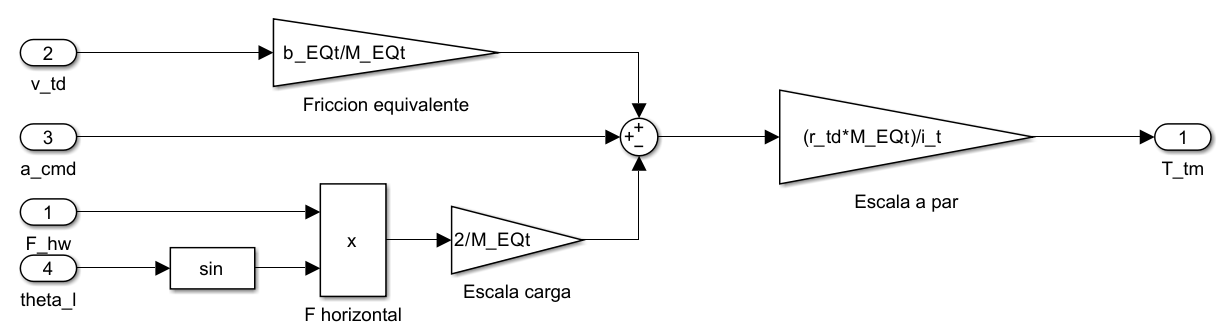
\includegraphics[width=0.88\linewidth]{imagenes_informe/usuario/CR_carro4.png}
\caption{Cálculo del torque del motor del carro a partir de la aceleración comandada, la fricción equivalente y la tensión horizontal del cable.}
\label{fig:cr-torque-carro}
\end{figure}
	
	La estructura implementada puede escribirse como
	\begin{align}
		v_c&=v^*+K_x(x_t^*-x_t)+v_{sw},\\
		e_v&=v_c-\dot x_t,\qquad
		a_{cmd}=a^*+K_{pv}e_v+K_{iv}\int e_v\,dt.
	\end{align}

\begin{figure}[H]
\centering
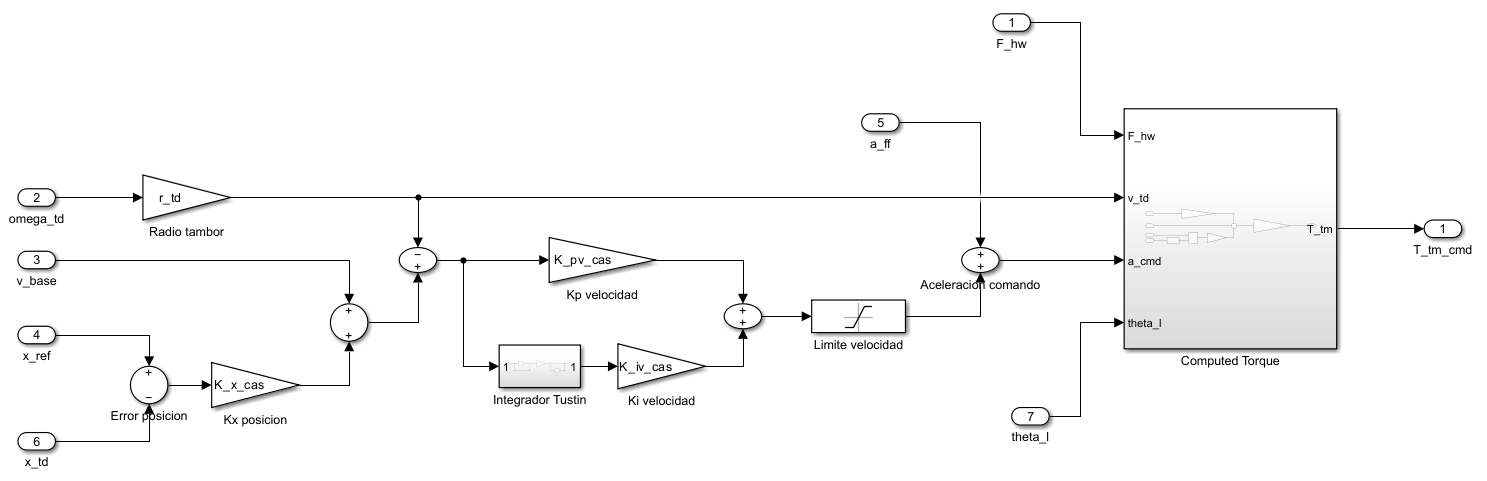
\includegraphics[width=0.96\linewidth]{imagenes_informe/usuario/CR_carro3.png}
\caption{Implementación de la cascada de posición y velocidad del carro y cálculo de la aceleración comandada.}
\label{fig:cr-cascada-carro}
\end{figure}
	\paragraph{Lazo de velocidad y asignación de polos.}
	Para obtener la transferencia de velocidad se toma $v_{sw}=0$ y $a^*=0$, de modo que se estudia la respuesta de $v_c$ a través del PI. Si $V(s)=sX_t(s)$, la planta compensada satisface $sV(s)=A_{cmd}(s)$. El controlador, con condiciones iniciales nulas, cumple
	\begin{equation}
		A_{cmd}(s)=\left(K_{pv}+\frac{K_{iv}}{s}\right)[V_c(s)-V(s)].
	\end{equation}
	Al sustituirlo en la planta y multiplicar por $s$ se llega a
	\begin{equation}
		(s^2+K_{pv}s+K_{iv})V(s)=(K_{pv}s+K_{iv})V_c(s).
	\end{equation}
	Por consiguiente, la transferencia cerrada es
	\begin{equation}
		G_v(s)=\frac{V(s)}{V_c(s)}=\frac{K_{pv}s+K_{iv}}{s^2+K_{pv}s+K_{iv}}.
		\label{eq:polos-carro}
	\end{equation}
	Se eligen dos polos reales $p_f=-\lambda_f$ y $p_i=-\lambda_i$, con $\lambda_f>\lambda_i>0$. Al expandir $(s+\lambda_f)(s+\lambda_i)$ e igualarlo con el denominador de \eqref{eq:polos-carro}, resultan
	\begin{equation}
		K_{pv}=\lambda_f+\lambda_i,\qquad K_{iv}=\lambda_f\lambda_i.
	\end{equation}
	El polo rápido fija la respuesta inicial de velocidad; el lento proviene de la acción integral. El lazo exterior tiene, bajo seguimiento ideal de velocidad, un polo aproximado $-K_x$. Una elección de diseño es ubicarlo por debajo de la banda principal del lazo interior, considerando además la frecuencia pendular. Los valores nominales $K_{pv}=2,40~\mathrm{s^{-1}}$ y $K_{iv}=0,20~\mathrm{s^{-2}}$ corresponden a polos $-2,314$ y $-0,0864~\mathrm{s^{-1}}$.
	
	\Needspace{5\baselineskip}
	
	\subsection{Referencia angular y corrección anti-sway}
	Para diseñar el anti-sway se considera una carga puntual suspendida de un apoyo que se desplaza con el carro. Este modelo de diseño se construye a partir de la geometría de un péndulo típico. Si $l$ es la distancia instantánea del apoyo a la carga,
	\begin{equation}
		x_l=x_t+l\sin\theta_l,\qquad y_l=Y_{t0}-l\cos\theta_l.
	\end{equation}
La figura~\ref{fig:carro_pendulo_EL} representa la geometría empleada en esta derivación. Las flechas de velocidad indican el sentido positivo de las componentes; $l$ es la longitud geométrica instantánea y $\theta_l$ se mide desde la vertical descendente hacia la carga.
\begin{figure}[H]
\centering
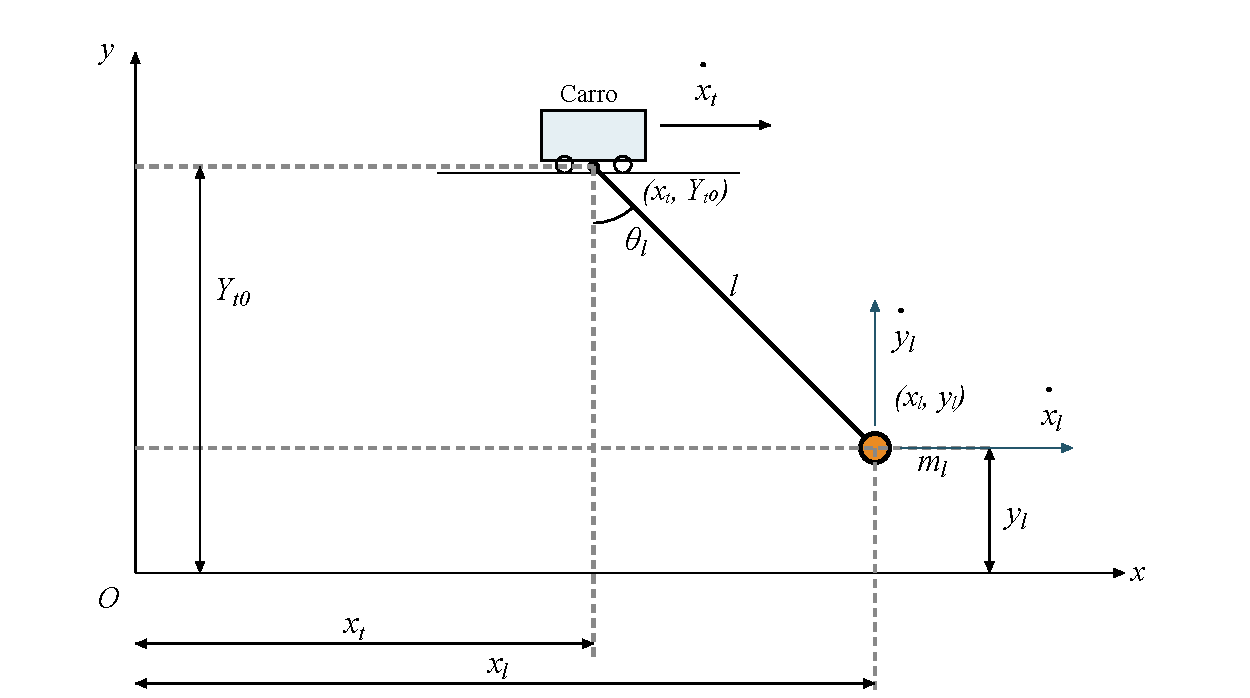
\includegraphics[width=0.82\linewidth]{imagenes_informe/modelo_planta/carro_pendulo_Euler_Lagrange.pdf}
\caption{Modelo cinemático carro--péndulo utilizado en la formulación de Euler--Lagrange.}
\label{fig:carro_pendulo_EL}
\end{figure}

	Se derivan las coordenadas para calcular la energía cinética de la masa suspendida $m_l$:
	\begin{align}
		\dot x_l&=\dot x_t+\dot l\sin\theta_l+l\dot\theta_l\cos\theta_l,\\
		\dot y_l&=-\dot l\cos\theta_l+l\dot\theta_l\sin\theta_l,\\
		\mathcal T&=\frac{m_l}{2}(\dot x_l^2+\dot y_l^2),\\
		\mathcal V&=m_lg(Y_{t0}-l\cos\theta_l).
	\end{align}
	La ecuación de Euler--Lagrange para $\theta_l$ da
	\begin{equation}
		l\ddot\theta_l+2\dot l\dot\theta_l+g\sin\theta_l
		=-\ddot x_t\cos\theta_l.
		\label{eq:pendulo-no-lineal}
	\end{equation}
	El término $2\dot l\dot\theta_l$ muestra que izar o descender modifica el balanceo; la aceleración $\ddot x_t$ es la excitación horizontal. Para diseñar a longitud casi constante se toma $\dot l\simeq0$; al linealizar \emph{solo para la asignación de ganancias} alrededor de ángulos pequeños,
	\begin{equation}
		\ddot\theta_l+\omega_p^2\theta_l\simeq-\frac{\ddot x_t}{l},
		\qquad\omega_p=\sqrt{g/l}.
		\label{eq:pendulo-lineal}
	\end{equation}
	Para la regulación, $l_h$ designa la longitud ordenada por la cinemática del tambor; $l$ sigue representando la longitud geométrica deformada de la planta. La frecuencia pendular empleada por el controlador se calcula con $l_h$.

	En cambio, el equilibrio de \eqref{eq:pendulo-no-lineal} bajo aceleración horizontal constante cumple $\tan\theta_{ref}=-a^*/g$. De ahí se usa una referencia angular variable:
	\begin{equation}
		\theta_{ref}=\operatorname{atan2}(-a^*,g),\qquad
		v_{sw}=2\zeta\omega_p l_h\,(\theta_l-\theta_{ref}),\qquad \omega_p=\sqrt{g/l_h}.
		\label{eq:antisway}
	\end{equation}

\begin{figure}[H]
\centering
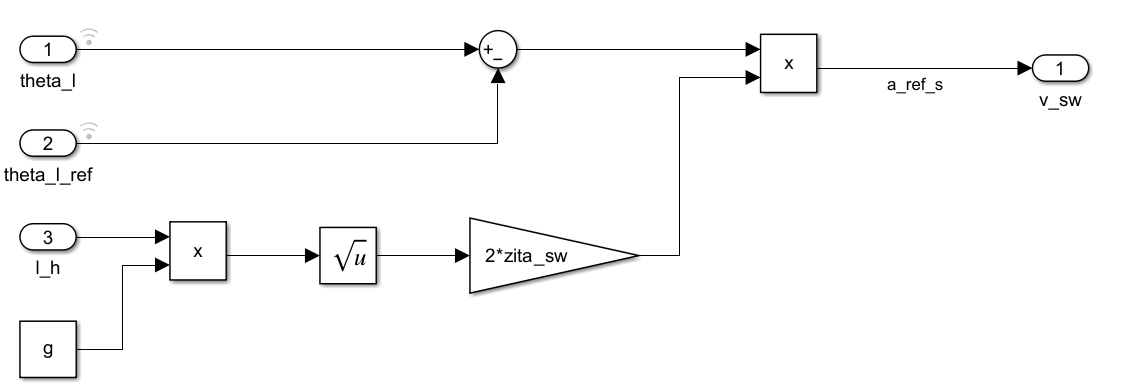
\includegraphics[width=0.88\linewidth]{imagenes_informe/usuario/CR_carroSW5.png}
\caption{Implementación de la corrección anti-sway a partir del error angular y de la longitud del cable.}
\label{fig:cr-antisway}
\end{figure}
	Para una referencia angular fija se define $e_\theta=\theta_l-\theta_{ref}$. Si el carro siguiera instantáneamente la corrección, se tendría $\ddot x_t\simeq\dot v_{sw}=2\zeta\omega_p l_h\,\dot e_\theta$. Al sustituir en \eqref{eq:pendulo-lineal}, el péndulo ideal satisface
	\begin{equation}
		\ddot e_\theta+2\zeta\omega_p\,\dot e_\theta+\omega_p^2e_\theta\simeq0,
	\end{equation}
	Con una referencia variable, la magnitud de seguimiento angular es $\theta_l-\theta_{ref}(t)$.
	
	\Needspace{5\baselineskip}
	
	\subsection{Modelo y asignación de polos del izaje}
	Se parte de la cinemática y de los balances de torque de la guía (Ecs.~6.a--6.e). La altura nominal es $y_h=Y_{t0}-l_h$ y, por la relación de aparejo $2{:}1$, $2\dot y_h=r_{hd}\omega_{hd}$; de aquí $-2\dot l_h=r_{hd}\omega_{hd}$. La tensión aplica al tambor un torque $T_{hdl}=r_{hd}F_{hw}$. Los balances son
	\begin{align}
		J_{hd+hEb}\dot\omega_{hd}&=T_{hd}+T_{hEb}-b_{hd}\omega_{hd}-T_{hdl},\\
		J_{hm+hb}\dot\omega_{hm}&=T_{hm}+T_{hb}-b_{hm}\omega_{hm}-T_{hml},\\
		\omega_{hm}&=i_h\omega_{hd},\qquad T_{hd}=i_hT_{hml}.
	\end{align}
	Se sustituye la ecuación del motor en la del tambor y se agrupan los términos del eje lento. Con $J_h=J_{hd+hEb}+i_h^2J_{hm+hb}$ y $b_h=b_{hd}+i_h^2b_{hm}$ resulta
	\begin{equation}
		J_h\dot\omega_{hd}+b_h\omega_{hd}
		=i_h(T_{hm}+T_{hb})+T_{hEb}-r_{hd}F_{hw}.
	\end{equation}
	Finalmente, al reemplazar $\omega_{hd}=-2\dot l_h/r_{hd}$ y dividir por $r_{hd}$ se expresa la dinámica en longitud de cable:
	\begin{align}
		M_{\EQh}\ddot l_h+b_{\EQh}\dot l_h
		&=-\frac{i_h}{r_{hd}}(T_{hm}+T_{hb})
		-\frac{T_{hEb}}{r_{hd}}+F_{hw},\\
		M_{\EQh}&=\frac{2J_h}{r_{hd}^2},\qquad
		b_{\EQh}=\frac{2b_h}{r_{hd}^2}.
	\end{align}
En operación con frenos abiertos, $T_{hm}^*=T'_{hm}+(r_{hd}/i_h)F_{hw}$ desacopla nominalmente la tensión y deja $M_{\EQh}\ddot l_h+b_{\EQh}\dot l_h=-(i_h/r_{hd})T'_{hm}$. La ley implementada suma una acción anticipativa calculada con la velocidad y la aceleración deseadas, y una corrección por realimentación:
\begin{align}
T'_{hm}&=T_{ff,h}+T_{fb,h},\\
T_{ff,h}&=-\frac{r_{hd}}{i_h}\left(M_{\EQh}\ddot l_h^*+b_{\EQh}\dot l_h^*\right),\\
T_{fb,h}&=K_{hp}e_l+K_{hd}\dot e_l+K_{hi}\int e_l\,dt,\qquad e_l=l_h^*-l_h.
\end{align}
El término anticipativo compensa nominalmente la inercia y el rozamiento para la trayectoria solicitada. En el esquema de la figura~\ref{fig:cr-izaje}, el error de velocidad se integra para formar el error de longitud y se integra nuevamente para la acción integral; esta equivalencia supone condiciones iniciales coherentes. La tensión del cable se compensa por separado.

\begin{figure}[H]
\centering
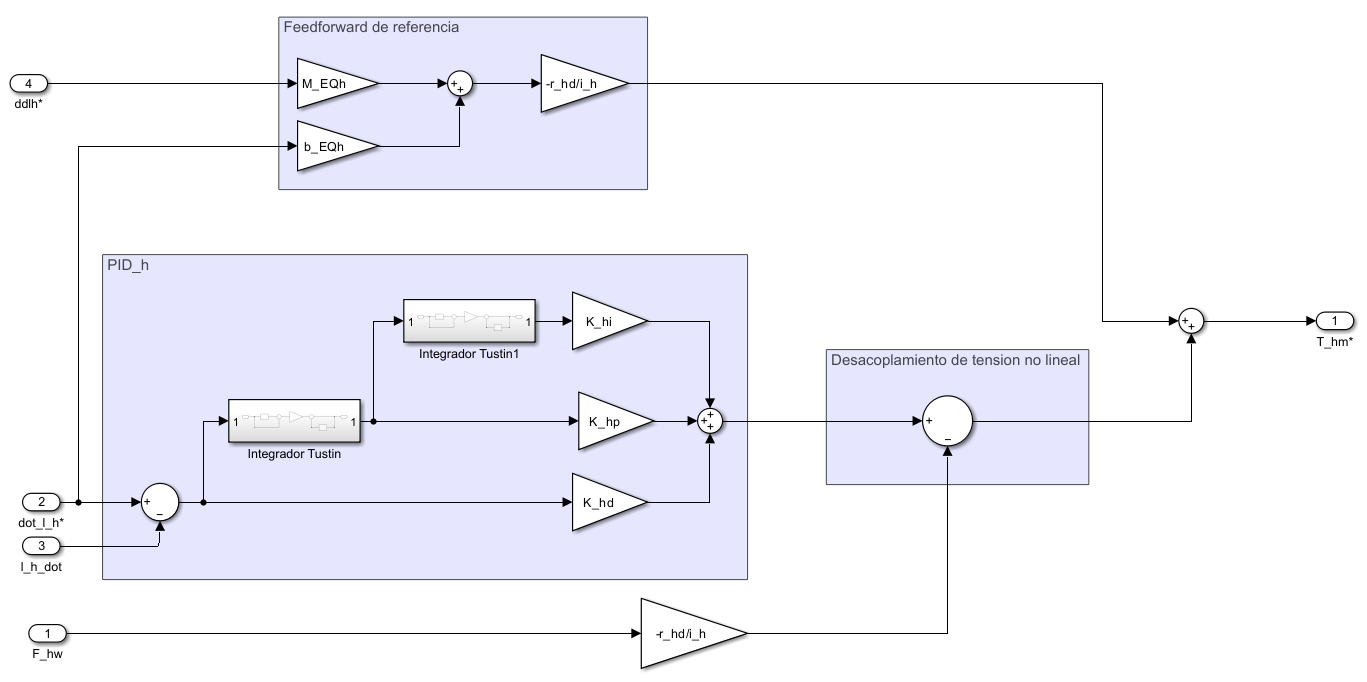
\includegraphics[width=0.94\linewidth]{imagenes_informe/usuario/CR_iz2.png}
\caption{Implementación del regulador de izaje: anticipación de velocidad y aceleración, realimentación PID y compensación de tensión.}
\label{fig:cr-izaje}
\end{figure}

En Laplace, con condiciones iniciales nulas,
	\begin{equation}
	(M_{\EQh}s^2+b_{\EQh}s)L_h
	=-\frac{i_h}{r_{hd}}\left[T_{ff,h}(s)+\left(K_{hd}s+K_{hp}+\frac{K_{hi}}s\right)(L_h^*-L_h)\right].
	\end{equation}
	Como $T_{ff,h}$ depende solo de la referencia, no modifica el polinomio característico de la realimentación. Al reunir los términos en $L_h$ y multiplicar por $s$, se obtiene dicho polinomio. Para abreviar se definen $\alpha_h=i_h/(r_{hd}M_{\EQh})$ y $\beta_h=b_{\EQh}/M_{\EQh}$. Entonces
	\begin{equation}
		P_h(s)=s^3+(\beta_h-\alpha_hK_{hd})s^2
		-\alpha_hK_{hp}s-\alpha_hK_{hi}.
	\end{equation}
	Se asigna $P_d(s)=(s+\omega_{posh})(s^2+2\zeta_h\omega_{posh}s+\omega_{posh}^2)$, con $n_h=2\zeta_h+1$. La expansión del polinomio deseado tiene coeficientes $n_h\omega_{posh}$, $n_h\omega_{posh}^2$ y $\omega_{posh}^3$. Igualándolos con los de $P_h(s)$, y definiendo $c_h=r_{hd}M_{\EQh}/i_h$, resultan
	\begin{align}
		K_{hp}&=-c_hn_h\omega_{posh}^2,\\
		K_{hi}&=-c_h\omega_{posh}^3,\\
		K_{hd}&=\frac{r_{hd}}{i_h}b_{\EQh}-c_hn_h\omega_{posh}.
	\end{align}
	
	Se fijaron los valores de diseño en: $n_h=2,7$ y $\omega_{posh}=1,8~\mathrm{rad/s}$, de modo que $\zeta_h=0,85$. La asignación nominal produce un polo real en $-1,8~\mathrm{s^{-1}}$ y un par conjugado en $-1,53\pm j\,0,948~\mathrm{s^{-1}}$, representados en la figura~\ref{fig:polos-izaje-nominal}. Estos son polos del modelo reducido utilizado para el diseño.

\begin{figure}[H]
\centering
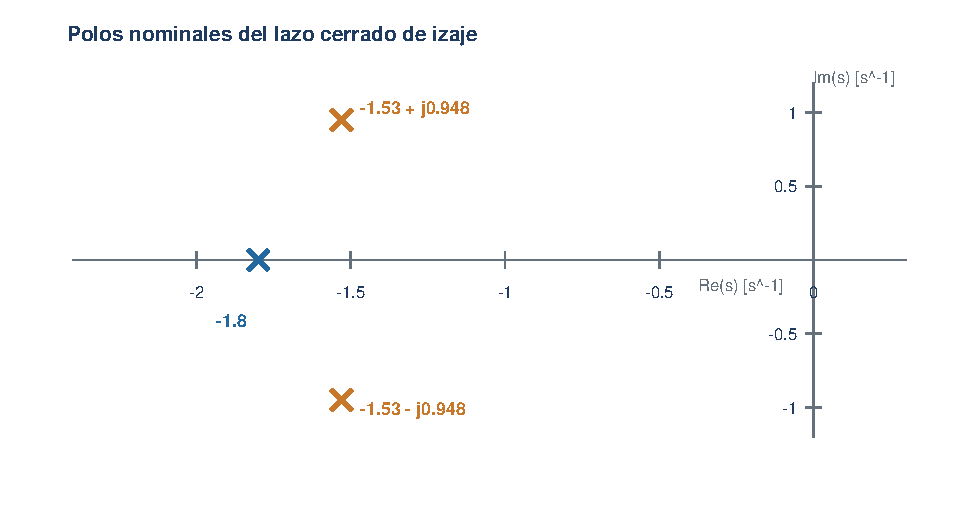
\includegraphics[width=0.86\linewidth]{imagenes_informe/usuario/ensayos_regulatorios_aislados/polos_izaje_nominal.pdf}
\caption{Polos nominales del lazo de izaje asignados con $n_h=2,7$ y $\omega_{posh}=1,8~\mathrm{rad/s}$.}
\label{fig:polos-izaje-nominal}
\end{figure}

La evaluación experimental de estas leyes, con referencias aisladas, se presenta en el apartado~\ref{subsec:validacion_regulatoria_MIL}. La integración con las referencias y secuencias del supervisor se evalúa en la sección~\ref{sec:integracion_p1}.

\par
\Needspace{10\baselineskip}
\section{Autómata supervisor y generación de referencias}
\label{sec:supervisor_MIL}
Esta sección presenta el supervisor y sus funciones de generación de referencias en MATLAB, Simulink y Stateflow. La realización de los autómatas en CODESYS se desarrolla por separado en la sección~\ref{sec:implementacion_codesys}.

\Needspace{5\baselineskip}

\subsection{Estructura general}
El autómata supervisor se implementa como un diagrama Stateflow con cinco regiones paralelas. La región \texttt{INTERLOCKS} se ejecuta en primer lugar y acondiciona las entradas, calcula aceleraciones, límites normales, comprobaciones de torque, códigos auxiliares y banderas comunes. En segundo lugar se ejecuta \texttt{CARGA\_Y\_TWISTLOCKS}, que controla la toma, el pesaje y la liberación. \texttt{OPERACION} se ejecuta en tercer lugar y administra los modos principales. Luego se ejecuta \texttt{FRENOS}, que contiene en paralelo las máquinas del carro y del izaje. Finalmente, \texttt{DIAGNOSTICO} actualiza los códigos de alarma y falla.

El paralelismo permite que las secuencias de carga y frenos continúen supervisándose mientras cambia el modo de operación. Las regiones comparten variables locales y salidas; por ello, el orden indicado resulta relevante. En particular, \texttt{INTERLOCKS} calcula las banderas que posteriormente consumen las regiones de carga, operación y diagnóstico durante la misma activación del chart.

\begin{figure}[!htb]
    \centering
    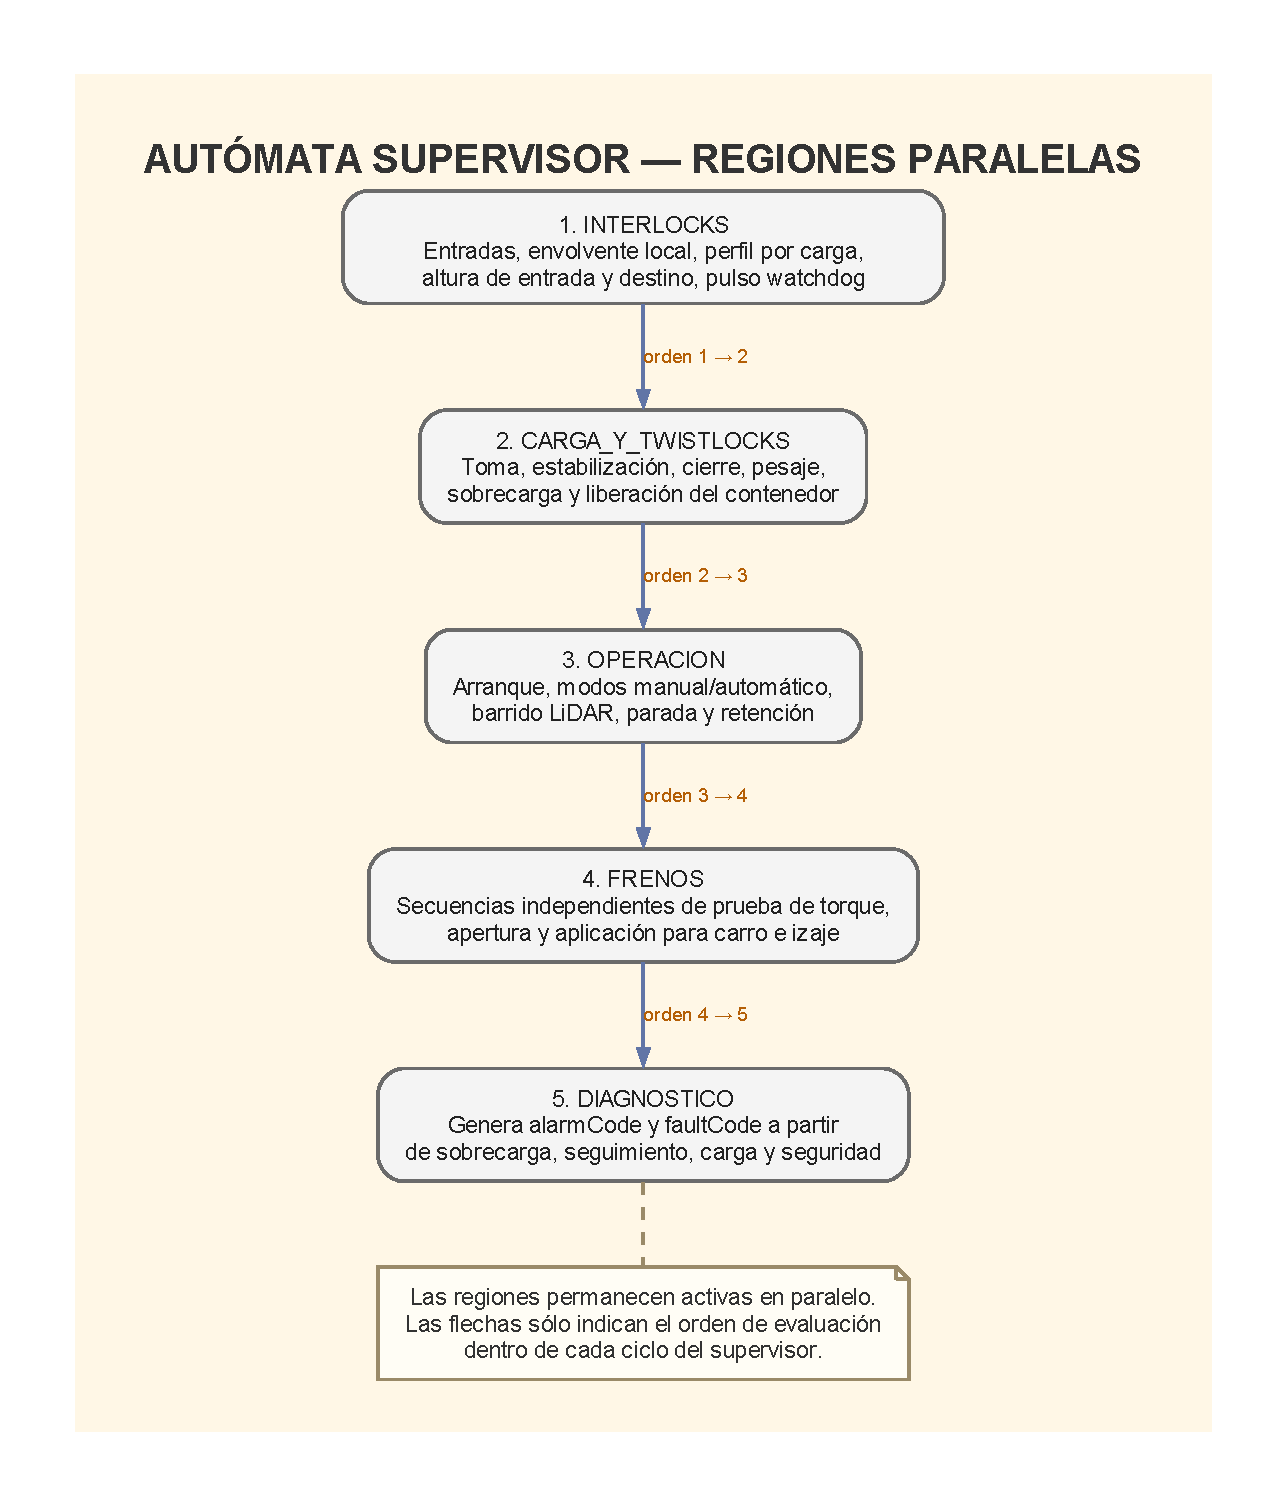
\includegraphics[height=0.72\textheight,keepaspectratio]{imagenes_informe/otro/diagramas_automatas_revision/01_arquitectura_supervisor.pdf}
    \caption{Organización general, responsabilidades y orden de ejecución de las regiones paralelas del autómata supervisor.}
\label{fig:supervisor_arquitectura}
\end{figure}

\Needspace{5\baselineskip}

\subsection{Interfaz funcional del supervisor}
El supervisor constituye el vínculo entre las órdenes del operador, las mediciones de la planta, el nivel de seguridad y los reguladores. Sus entradas no representan mandos directos sobre los actuadores: se procesan para obtener condiciones lógicas, referencias limitadas y permisos internos. La \cref{tab:interfaz_supervisor} resume las señales que determinan las decisiones principales.

\Needspace{12\baselineskip}
\begin{longtable}{L{4.1cm} L{4.2cm} L{5.3cm}}
\caption{Interfaz funcional principal del autómata supervisor.}\label{tab:interfaz_supervisor}\\
\toprule
Grupo & Señales representativas & Utilización dentro del supervisor\\
\midrule
\endfirsthead
\toprule
Grupo & Señales representativas & Utilización dentro del supervisor\\
\midrule
\endhead
Órdenes & Marcha, parada, reinicio, selección manual/automática y orden de barrido & Selección de estados operativos y reconocimiento de fallas.\\
Mandos manuales & \textit{Joystick} horizontal, \textit{joystick} vertical y órdenes de \textit{twistlocks} & Generación de referencias manuales y secuencia de toma o liberación.\\
Movimiento & Posición, velocidad y aceleración de carro e izaje & Seguimiento de trayectoria, transferencias sin salto y aplicación de frenos.\\
Carga suspendida & Ángulo, velocidad angular, tensión, contacto y confirmación de \textit{twistlocks} & Estabilización, pesaje, detección de cuerda floja y estado de carga.\\
Perfil & Posición del LIDAR, altura medida y memoria del perfil & Registro del barrido, validación de cobertura y cálculo de la superficie objetivo.\\
Seguridad & Permisos global, de carro y de izaje & Habilitación de movimientos, parada normal y retención de falla.\\
Salidas de referencia & $x^*$, $v_x^*$, $a_x^*$, $y^*$, $v_y^*$ y $a_y^*$ & Consignas entregadas al nivel regulatorio.\\
Salidas discretas & Órdenes de freno, \textit{twistlocks}, códigos, estado y pulso de \textit{watchdog} & Accionamiento secuencial, diagnóstico, HMI y vigilancia desde el nivel de seguridad.\\
\bottomrule
\end{longtable}

\Needspace{5\baselineskip}

\subsection{Generación de trayectorias y referencias coordinadas}
\label{subsec:trayectorias_supervisor}
El planificador forma parte de las funciones del supervisor: transforma el objetivo del operador y el perfil disponible en referencias coordinadas para ambos ejes. Los límites aquí descritos corresponden a la revisión documentada del planificador. Los ensayos MIL de la sección~\ref{sec:integracion_p1} declaran su configuración particular; los valores de una revisión no deben extrapolarse a todas las corridas.

\Needspace{5\baselineskip}

\subsubsection{Objetivo de la planificación}
En modo automático el operador proporciona principalmente la posición horizontal final. La función de envolvente local dilata el perfil relevado tomando el máximo de cada celda y sus vecinas inmediatas. La función de superficie objetivo consulta el máximo de las celdas de esa envolvente solapadas por el ancho de $2.44~\mathrm{m}$ del contenedor. La altura de aproximación se obtiene como
\begin{equation}
y_{auto}=y_{env}(x^*)+H_c(1+\delta_{carga})+\Delta l_{est},\qquad H_c=2.59~\mathrm{m},
\label{eq:objetivo_local_vigente}
\end{equation}
donde $\delta_{carga}$ vale uno con contenedor y cero con \textit{spreader} vacío. El estiramiento se calcula con la masa suspendida limitada entre $15000$ y $65000~\mathrm{kg}$ y la rigidez del cable evaluada a partir de la altura base. Esta revisión utiliza un margen fijo de una altura de contenedor; \texttt{finalApproachDistance} permanece en la interfaz, pero no interviene en \texttt{calcularObjetivoSeguro}.

La trayectoria automática debe elevar y trasladar simultáneamente, respetar las cotas de obstáculos y terminar con velocidad y aceleración nulas.


\Needspace{5\baselineskip}


\subsubsection{Línea de seguridad}
La línea de seguridad implementada se calcula mediante
\begin{equation}
y_{seg}=\max\left(y_{manual\rightarrow auto},\min(40,\max_i y_{perfil,i}+2H_c)\right).
\label{eq:safetyline}
\end{equation}
El desplazamiento de dos alturas de contenedor equivale a $5.18~\mathrm{m}$. La línea se dibuja en la visualización y permite calcular \texttt{clearanceOK}, pero esta bandera no se utiliza en las guardas de entrada al automático ni para deshabilitar el anti-sway. El generador conserva además una cota alta de cruce no menor que el máximo de la envolvente más $5.18~\mathrm{m}$.

Para verificar el despeje se descuenta el estiramiento del cable calculado con \eqref{eq:stretch}. La condición calculada por \texttt{calcularDespeje} es
\begin{equation}
y_l-\Delta l\geq y_{seg}.
\end{equation}
Esta comprobación global se distingue de \texttt{autoEntryHeightOK}, que compara la altura medida del izaje con \texttt{calcularObjetivoSeguro} evaluado en la posición actual del carro.


Para ilustrar los perfiles se utiliza un único ejemplo del generador implementado: traslado desde el slot 6 ($x_0=-16.58~\mathrm{m}$) hasta el slot 23 ($x_f=24.90~\mathrm{m}$), con altura comandada inicial de $15~\mathrm{m}$, objetivo vertical de aproximación de $0.85~\mathrm{m}$ y masa suspendida de $50\,990~\mathrm{kg}$. Se toma como base el perfil relevado en el ensayo completo y se descuenta el contenedor retirado del origen. Los dos ejes parten del reposo. Las figuras siguientes muestran las referencias del plan, sin simular la respuesta de la planta; la compuerta de descenso se considera satisfecha al finalizar el traslado horizontal. El tiempo total del ejemplo es $57.66~\mathrm{s}$.

\Needspace{5\baselineskip}

\subsubsection{Perfil horizontal}
El movimiento horizontal utiliza rampas senoidales de aceleración, un tramo de velocidad constante y una rampa de frenado. Se adoptan
\begin{equation}
v_{x\max}=2.5~\mathrm{m/s},\quad a_{x\max}=0.3~\mathrm{m/s^2},\quad j_{x\max}=0.5~\mathrm{m/s^3}.
\end{equation}
Si la distancia es suficiente, el perfil alcanza la velocidad máxima. Si es corta, se reduce la velocidad de crucero. La duración de la rampa se selecciona como
\begin{equation}
T_r=\max\left(0.25,\frac{\pi v_c}{2a_{x\max}},\pi\sqrt{\frac{v_c}{2j_{x\max}}}\right).
\end{equation}
Las rampas senoidales hacen que la aceleración comience y termine en cero, reduciendo la excitación de la carga suspendida.

\begin{figure}[H]
\centering
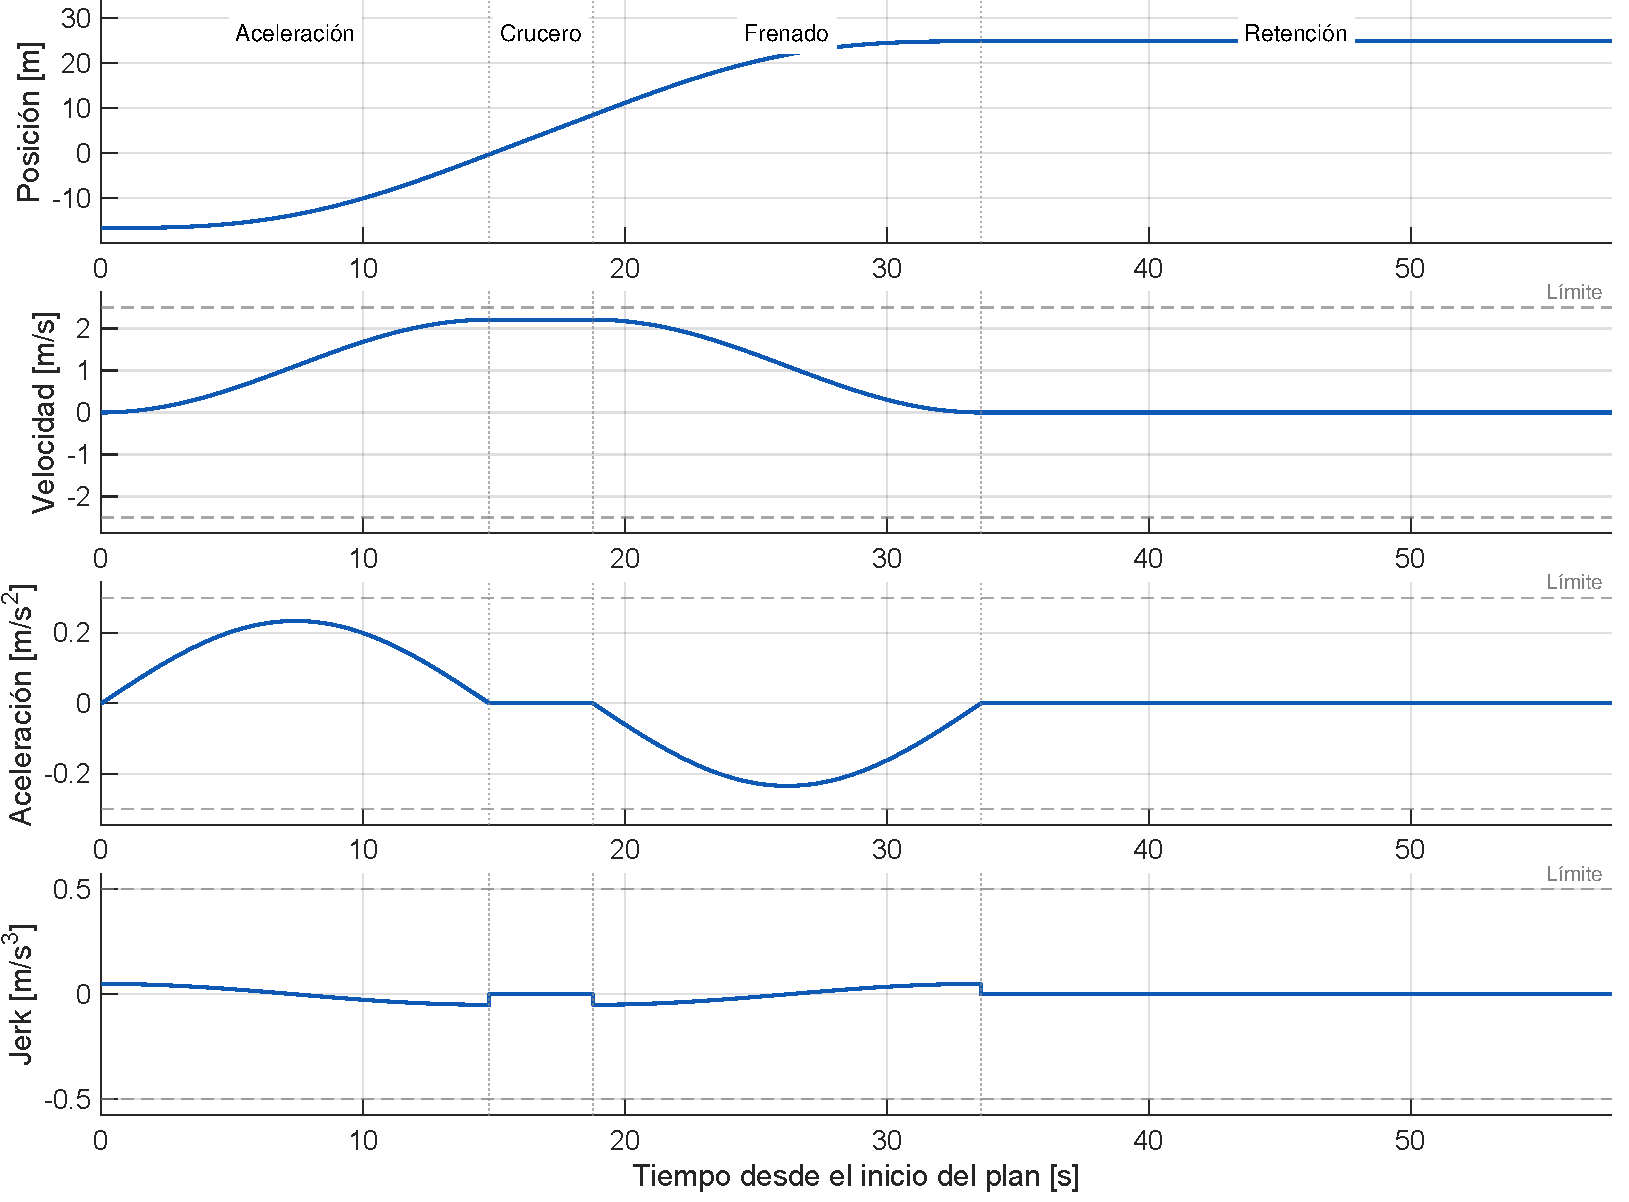
\includegraphics[width=.98\textwidth,height=.69\textheight,keepaspectratio]{imagenes_informe/trayectorias/perfil_horizontal.pdf}
\caption{Referencias horizontales del ejemplo: posición, velocidad, aceleración y jerk. Las líneas discontinuas indican los límites de diseño y las divisiones verticales separan aceleración, crucero, frenado y retención.}
\label{fig:trayectoria_horizontal}
\end{figure}

El movimiento horizontal termina a los $33.58~\mathrm{s}$ y después mantiene la posición objetivo mientras finaliza el izaje. En este plan, la velocidad de crucero es $2.210~\mathrm{m/s}$ y los máximos absolutos de aceleración y jerk son $0.2344~\mathrm{m/s^2}$ y $0.0497~\mathrm{m/s^3}$. El ajuste de la duración horizontal para lograr despeje permite respetar los límites indicados.


\Needspace{5\baselineskip}


\subsubsection{Perfil vertical quíntico}
Para el izaje se utilizan polinomios de quinto orden:
\begin{equation}
p(t)=c_0+c_1t+c_2t^2+c_3t^3+c_4t^4+c_5t^5.
\end{equation}
Los coeficientes se calculan imponiendo posición, velocidad y aceleración inicial y final. La duración mínima se busca de forma iterativa hasta verificar los límites de velocidad, aceleración y \textit{jerk}. Se utilizan $a_{y\max}=0.25~\mathrm{m/s^2}$ y $j_{y\max}=0.10~\mathrm{m/s^3}$ para el movimiento automático. El límite de $0.05~\mathrm{m/s^2}$ corresponde a la aproximación final manual.

El perfil vertical se divide en una fase ascendente y otra descendente. La fase de descenso comienza cuando la envolvente horizontal abandonó la zona de obstáculos y el carro está en condiciones de posicionamiento.

\begin{figure}[H]
\centering
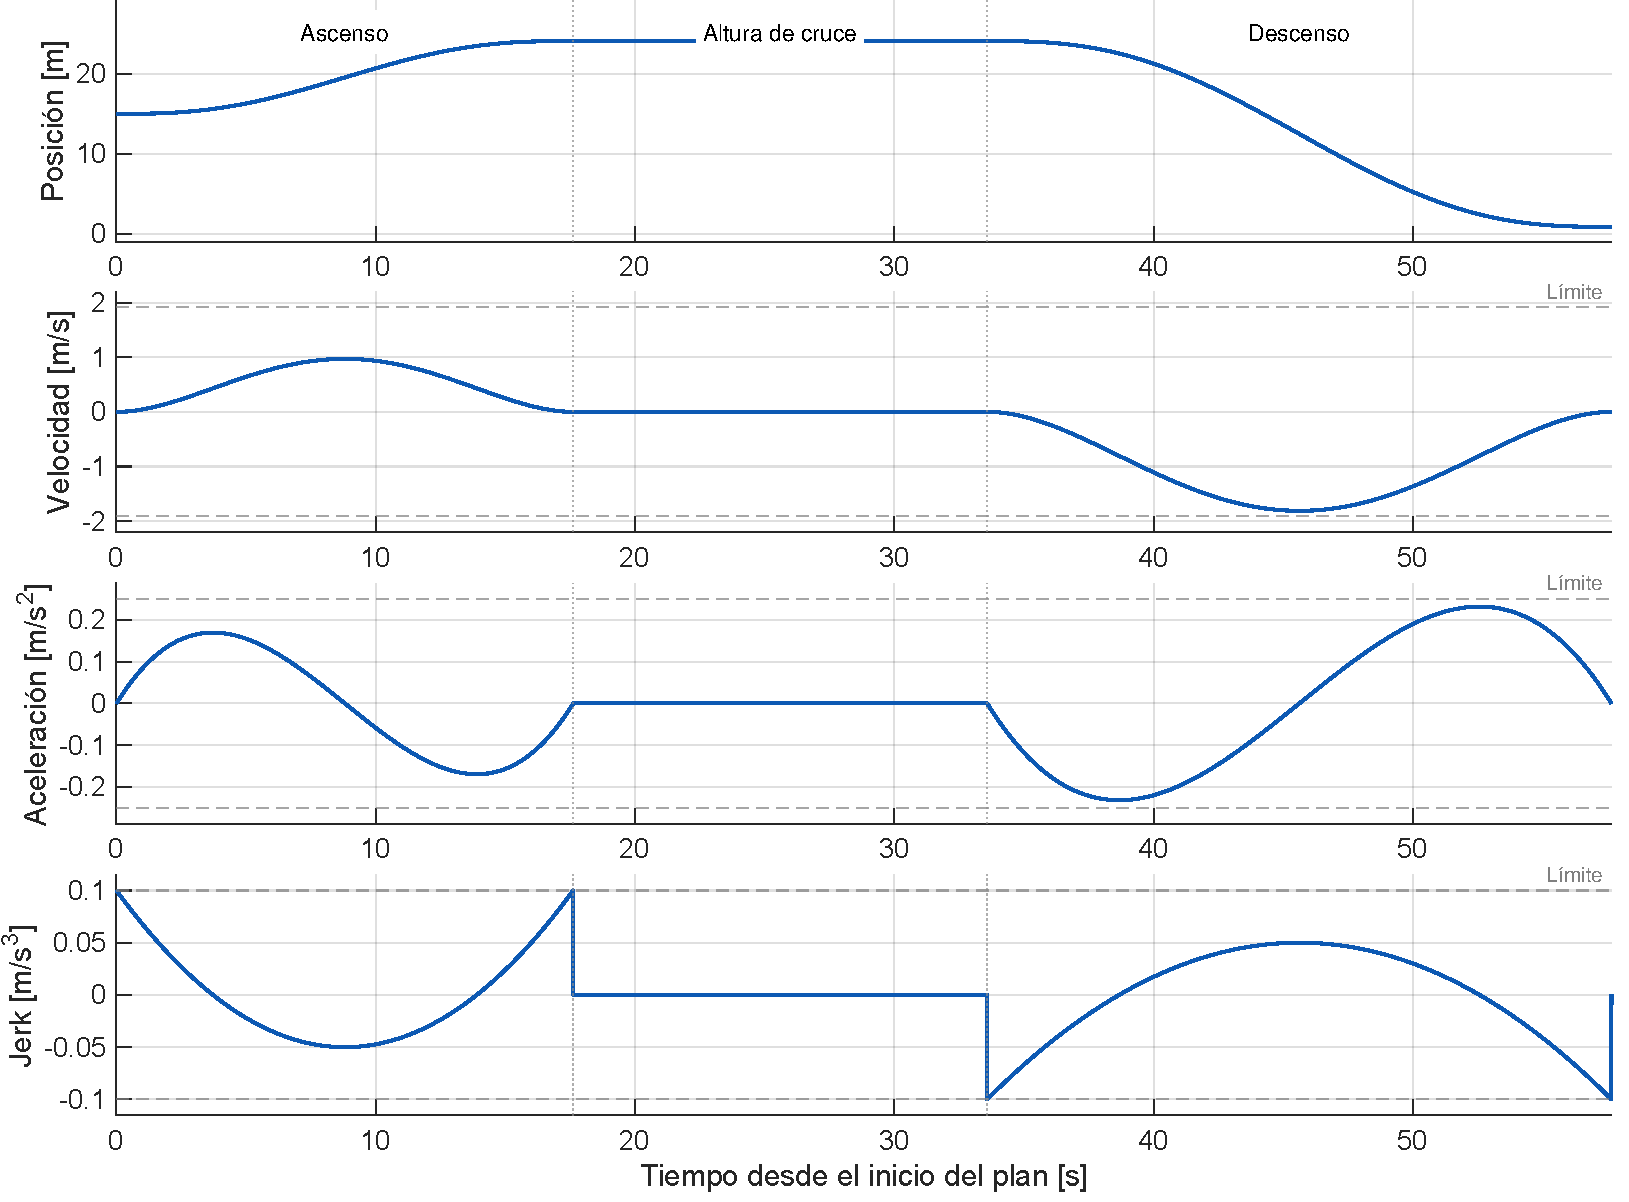
\includegraphics[width=.98\textwidth,height=.69\textheight,keepaspectratio]{imagenes_informe/trayectorias/perfil_vertical.pdf}
\caption{Referencias verticales del mismo plan: altura comandada, velocidad, aceleración y jerk. Se distinguen ascenso, mantenimiento de la altura de cruce y descenso hacia la cota de aproximación.}
\label{fig:trayectoria_vertical}
\end{figure}

El ascenso alcanza $24.11~\mathrm{m}$ a los $17.62~\mathrm{s}$. Esa altura se conserva hasta el fin del traslado horizontal, a los $33.58~\mathrm{s}$; luego comienza el descenso, de $24.08~\mathrm{s}$ de duración. El límite de velocidad cargada resulta $1.912~\mathrm{m/s}$ para la masa del ejemplo, y el máximo del plan es $1.812~\mathrm{m/s}$. La aceleración máxima es $0.2317~\mathrm{m/s^2}$ y el jerk máximo es $0.1000~\mathrm{m/s^3}$. Los enlaces conservan posición, velocidad y aceleración; el jerk está acotado y puede cambiar al pasar de un tramo a otro.


\Needspace{5\baselineskip}


\subsubsection{Coordinación simultánea}
El movimiento horizontal y el izaje comienzan en $t=0$. Antes de aceptar el plan se muestrea la trayectoria y se verifica que la base de la carga se mantenga por encima del perfil más el margen vertical. Si el carro alcanzaría un obstáculo demasiado pronto, se aumenta la duración horizontal por un factor $1.025$ y se repite la verificación.

Este procedimiento no demora intencionalmente el inicio del carro. En cambio, reduce su avance solamente lo necesario para que el izaje gane altura. Una vez alcanzada la zona libre, la trayectoria recupera el tramo de velocidad constante. Esta coordinación superpone los movimientos de izaje y traslación. Su efecto sobre la duración de la maniobra debe evaluarse con la configuración y los resultados de cada ensayo.

\begin{figure}[H]
\centering
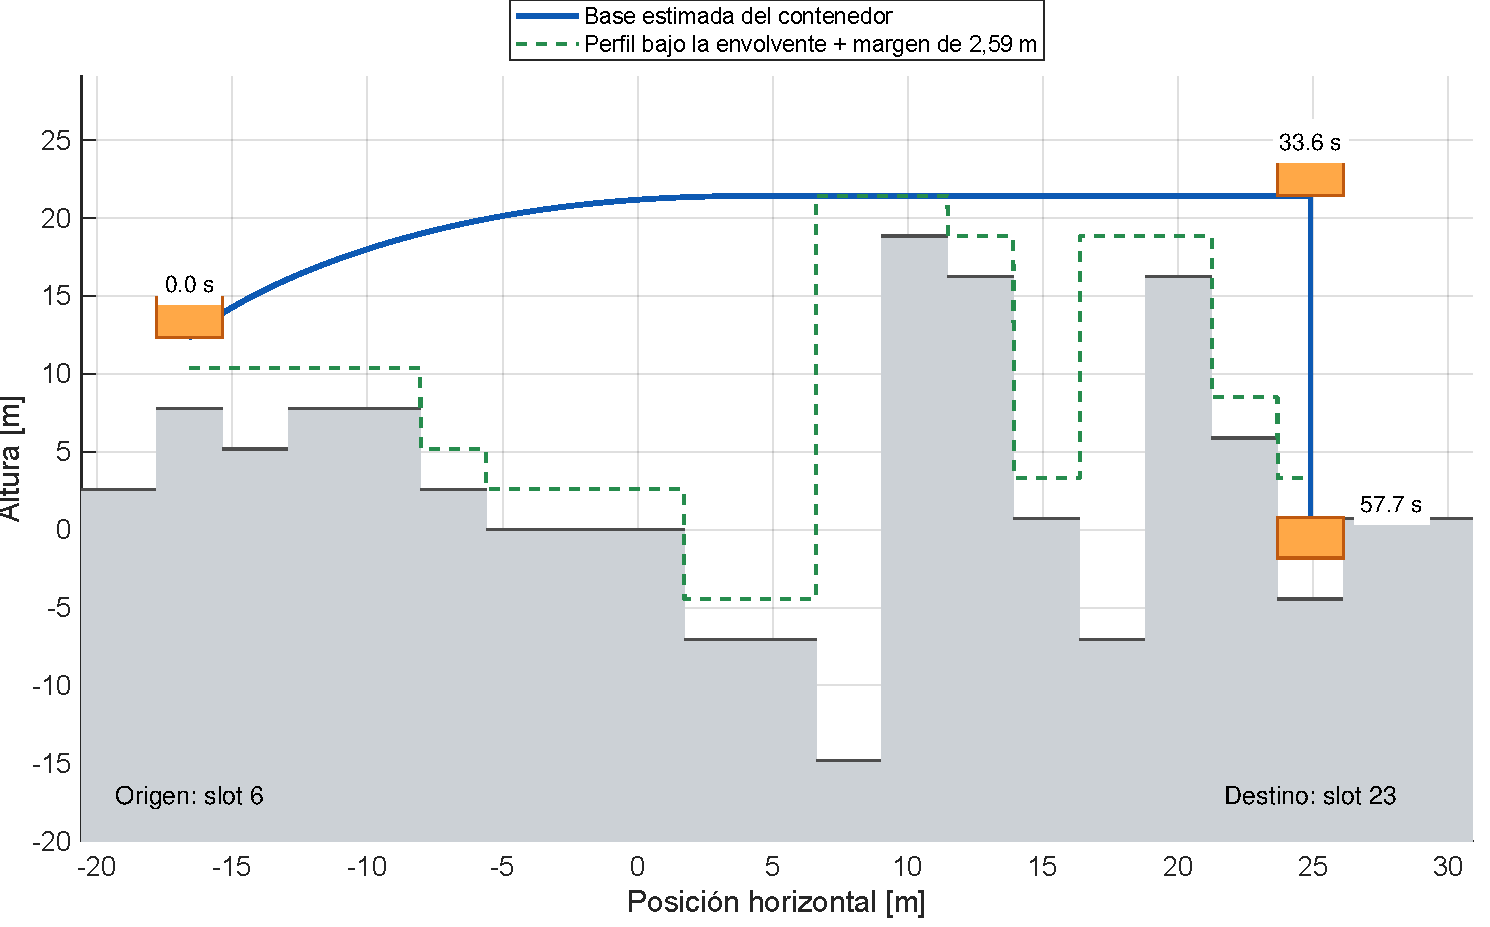
\includegraphics[width=.98\textwidth,height=.69\textheight,keepaspectratio]{imagenes_informe/trayectorias/coordinacion_xy.pdf}
\caption{Recorrido del ejemplo sobre el perfil disponible después de la toma.}
\label{fig:trayectoria_coordinada}
\end{figure}

La trayectoria geométrica del ejemplo se obtiene como $y_{\mathrm{base,plan}}=y_{\mathrm{ref}}-\Delta l-h_c$, con $h_c=2.59~\mathrm{m}$ y estiramiento cuasiestático de planificación $\Delta l=0.0805~\mathrm{m}$. Durante el transporte horizontal, la base permanece por encima de la cota exigida bajo toda la envolvente. Al alcanzar el destino, el carro mantiene su posición y se realiza el descenso hacia la altura de aproximación, sin representar todavía el contacto ni la entrega. La línea verde corresponde al criterio de cruce; no exige mantener esa separación durante el descenso final.


\Needspace{5\baselineskip}


\subsubsection{Verificación de colisión}
La envolvente horizontal se amplía con medio ancho de contenedor y un margen adicional de $2.59~\mathrm{m}$. El margen vertical \texttt{VERTICAL\_MARGIN} también vale $2.59~\mathrm{m}$ en el generador vigente. En cada muestra del plan se calcula la cota del obstáculo debajo de la carga. La condición de seguridad es
\begin{equation}
y_l-\Delta l-h_c\geq y_{obs}(x_l)+d_v.
\end{equation}
El plan se declara inválido si no puede cumplir esta condición antes del tiempo máximo. En ese caso, las referencias se fijan en el estado medido y no se genera movimiento automático.

Este comportamiento es preferible a saturar la altura o ignorar un obstáculo, porque una trayectoria inviable queda convertida en una condición detenida y observable por el supervisor.



\Needspace{5\baselineskip}



\subsection{Región INTERLOCKS}
La región \texttt{INTERLOCKS} concentra los cálculos que deben estar disponibles antes de evaluar las restantes regiones paralelas. No constituye una secuencia de producción independiente, sino una etapa de acondicionamiento y generación de variables comunes. Su ejecución al comienzo de cada activación evita repetir operaciones en diferentes estados y proporciona una única interpretación de las señales de entrada.

Entre sus tareas se encuentran el cálculo de aceleraciones a partir de velocidades muestreadas, la detección de flancos de órdenes, la comprobación de límites normales, la validación de torque previo a la apertura de los frenos, la evaluación del error de seguimiento, el cálculo de la altura de despeje y la actualización de códigos auxiliares. La \cref{tab:interlocks_supervisor} relaciona las funciones principales con las regiones que utilizan sus resultados.

\begin{table}[!htb]
\centering
\caption{Resultados principales generados por \texttt{INTERLOCKS}.}\label{tab:interlocks_supervisor}
\begin{tabular}{L{4.5cm} L{5.0cm} L{4.2cm}}
\toprule
Resultado & Criterio general & Consumidor principal\\
\midrule
Aceleraciones medidas & Diferencia discreta de velocidades & Operación y trayectoria\\
Límites normales & Comparación de posición y sentido solicitado & Mando manual y barrido\\
Torque comprobado & Torque disponible durante el estado de prueba & Máquinas de freno\\
\texttt{trackingFault} & Error sostenido de seguimiento & Operación y diagnóstico\\
Altura de aproximación & Envolvente local, carga, margen y estiramiento & Automático\\
\texttt{autoEntryHeightOK} & Perfil válido y altura local suficiente & Entrada al automático\\
\texttt{clearanceOK} & Despeje respecto de la línea global & Cálculo auxiliar; no es guarda de entrada\\
Códigos auxiliares & Combinación de condiciones activas & Diagnóstico y HMI\\
\bottomrule
\end{tabular}
\end{table}

La memoria \texttt{scannedObstacleProfile} se actualiza al cambiar \texttt{loadedState}, siempre que el perfil sea válido y no exista barrido activo: se resta $2.59~\mathrm{m}$ al tomar un contenedor y se suma la misma altura al liberarlo, en la celda asociada a la posición del carro. Luego se recalcula la envolvente local. Como carga se ejecuta después de \texttt{INTERLOCKS}, el cambio de estado cargado se incorpora al perfil en la siguiente activación.

\texttt{retenerSolicitudHMI} memoriza el flanco de solicitud de barrido recibido con el escaneo inactivo y lo conserva hasta parada, reinicio o secuencia completa. Esto permite atender un pulso del HMI una vez alcanzadas las condiciones de inicio.

Las operaciones indicadas se ejecutan durante cada ciclo del supervisor. En consecuencia, una modificación de una bandera calculada en \texttt{INTERLOCKS} puede ser utilizada por las regiones de carga y operación dentro de la misma activación del chart, siempre respetando el orden de ejecución configurado.

\Needspace{5\baselineskip}

\FloatBarrier
\Needspace{16\baselineskip}
\subsection{Indexación de estados de operación}
Para facilitar su utilización posterior se adopta la siguiente indexación funcional:
\Needspace{12\baselineskip}
\begin{longtable}{C{1.2cm} L{4.4cm} L{8.2cm}}
\caption{Estados de la región de operación.}\\
\toprule
Índice & Estado & Función principal\\
\midrule
\endfirsthead
\toprule
Índice & Estado & Función principal\\
\midrule
\endhead
O0 & \texttt{APAGADO} & Deshabilita reguladores y mantiene las referencias en la posición medida.\\
O1 & \texttt{ARRANQUE} & Inicia la secuencia, conserva frenos y espera permisos estables.\\
O2 & \texttt{LISTO} & Habilita reguladores con referencias detenidas y espera una selección.\\
O3 & \texttt{MANUAL\_SUPERVISADO} & Convierte los mandos del operador en referencias limitadas.\\
O4 & \texttt{BUMPLESS\_A\_AUTO} & Inicializa referencias con el estado medido antes del automático.\\
O5 & \texttt{AUTOMATICO} & Contiene planificación, ejecución y retención del objetivo.\\
O6 & \texttt{BUMPLESS\_A\_MANUAL} & Reduce las referencias en forma continua al abandonar automático.\\
O7 & \path{APROXIMACION_FINAL_MANUAL} & Mantiene $x$ y permite el mando vertical manual.\\
O8 & \path{PREPARAR_ESCANEO_LIDAR} & Eleva el conjunto y reinicia la memoria del perfil.\\
O9 & \texttt{IR\_EXTREMO\_DERECHO} & Traslada el carro vacío al inicio del barrido.\\
O10 & \path{BARRIDO_LIDAR_IZQUIERDA} & Retorna registrando el perfil.\\
O11 & \path{FINALIZAR_ESCANEO_LIDAR} & Detiene y valida la cobertura de los 33 \textit{slots}.\\
O12 & \texttt{PARADA\_NORMAL} & Lleva velocidades a cero respetando las rampas.\\
O13 & \texttt{RETENCION\_FALLA} & Deshabilita reguladores y retiene el sistema ante una falla.\\
\bottomrule
\end{longtable}

\Needspace{5\baselineskip}

\Needspace{.55\textheight}
\subsection{Estados APAGADO, ARRANQUE y LISTO}

\begin{figure}[H]
\centering
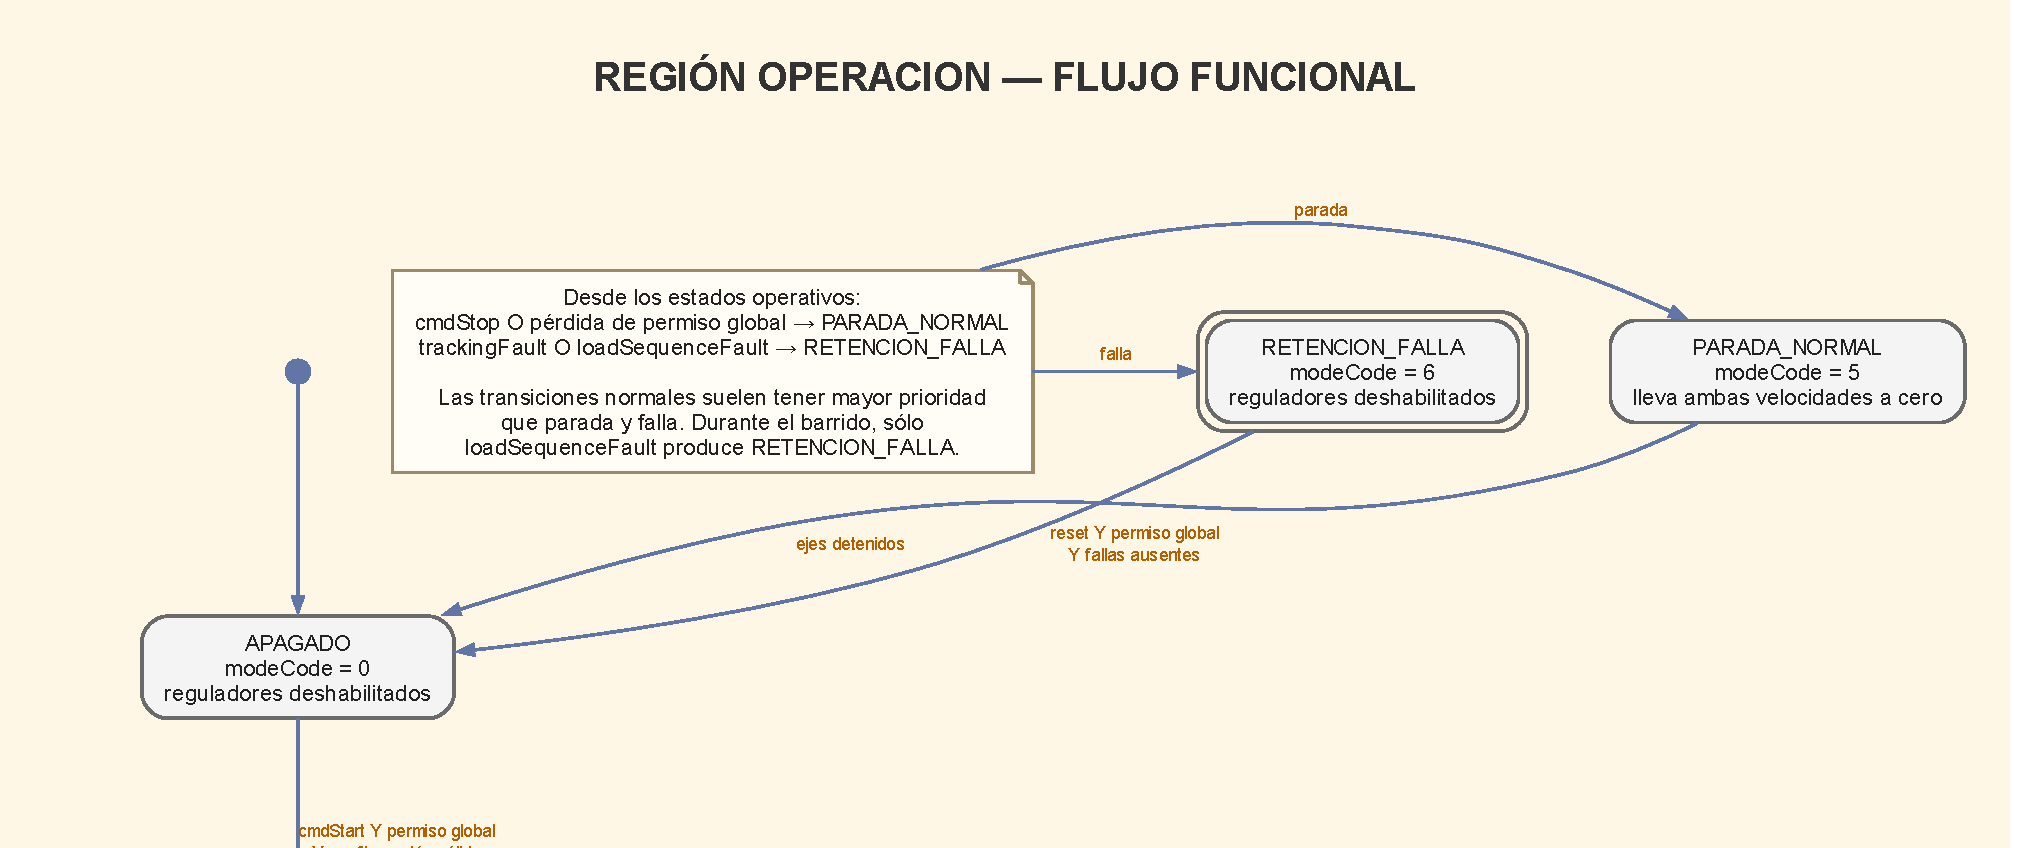
\includegraphics[width=.98\textwidth]{imagenes_informe/otro/diagramas_automatas_revision/02a_operacion_parada.pdf}
\caption{Región \texttt{OPERACION}: estado apagado y salidas comunes por parada o retención de falla. El arranque y los estados de maniobra se detallan en la \cref{fig:supervisor_operacion_maniobra}.}

\label{fig:supervisor_operacion_parada}
\end{figure}
\texttt{APAGADO} es el estado inicial. Su código de modo es cero y ambos reguladores quedan deshabilitados. La transición a \texttt{ARRANQUE} exige orden de marcha, permiso global y configuración válida.

\texttt{ARRANQUE} utiliza el código de modo uno. Durante este estado se mantiene el sistema sin referencias de movimiento y se verifica la disponibilidad de los permisos. Luego de cinco ciclos del supervisor, si carro e izaje están permitidos, se pasa a \texttt{LISTO}.

\texttt{LISTO} utiliza el código dos y habilita los reguladores con consignas detenidas. Posee transiciones hacia manual, automático, parada, retención de falla y barrido. La entrada a automático desde este estado es directa, sin pasar por \path{BUMPLESS_A_AUTO}, y exige \texttt{modeAutoReq}, \texttt{cmdAutoStart}, perfil válido, \texttt{autoEntryHeightOK} y ausencia de sobrecarga. La altura local se comprueba tanto con carga como con \textit{spreader} vacío; esta transición no exige \texttt{loadedState} ni ausencia de intervención manual.



\begin{figure}[H]
\centering
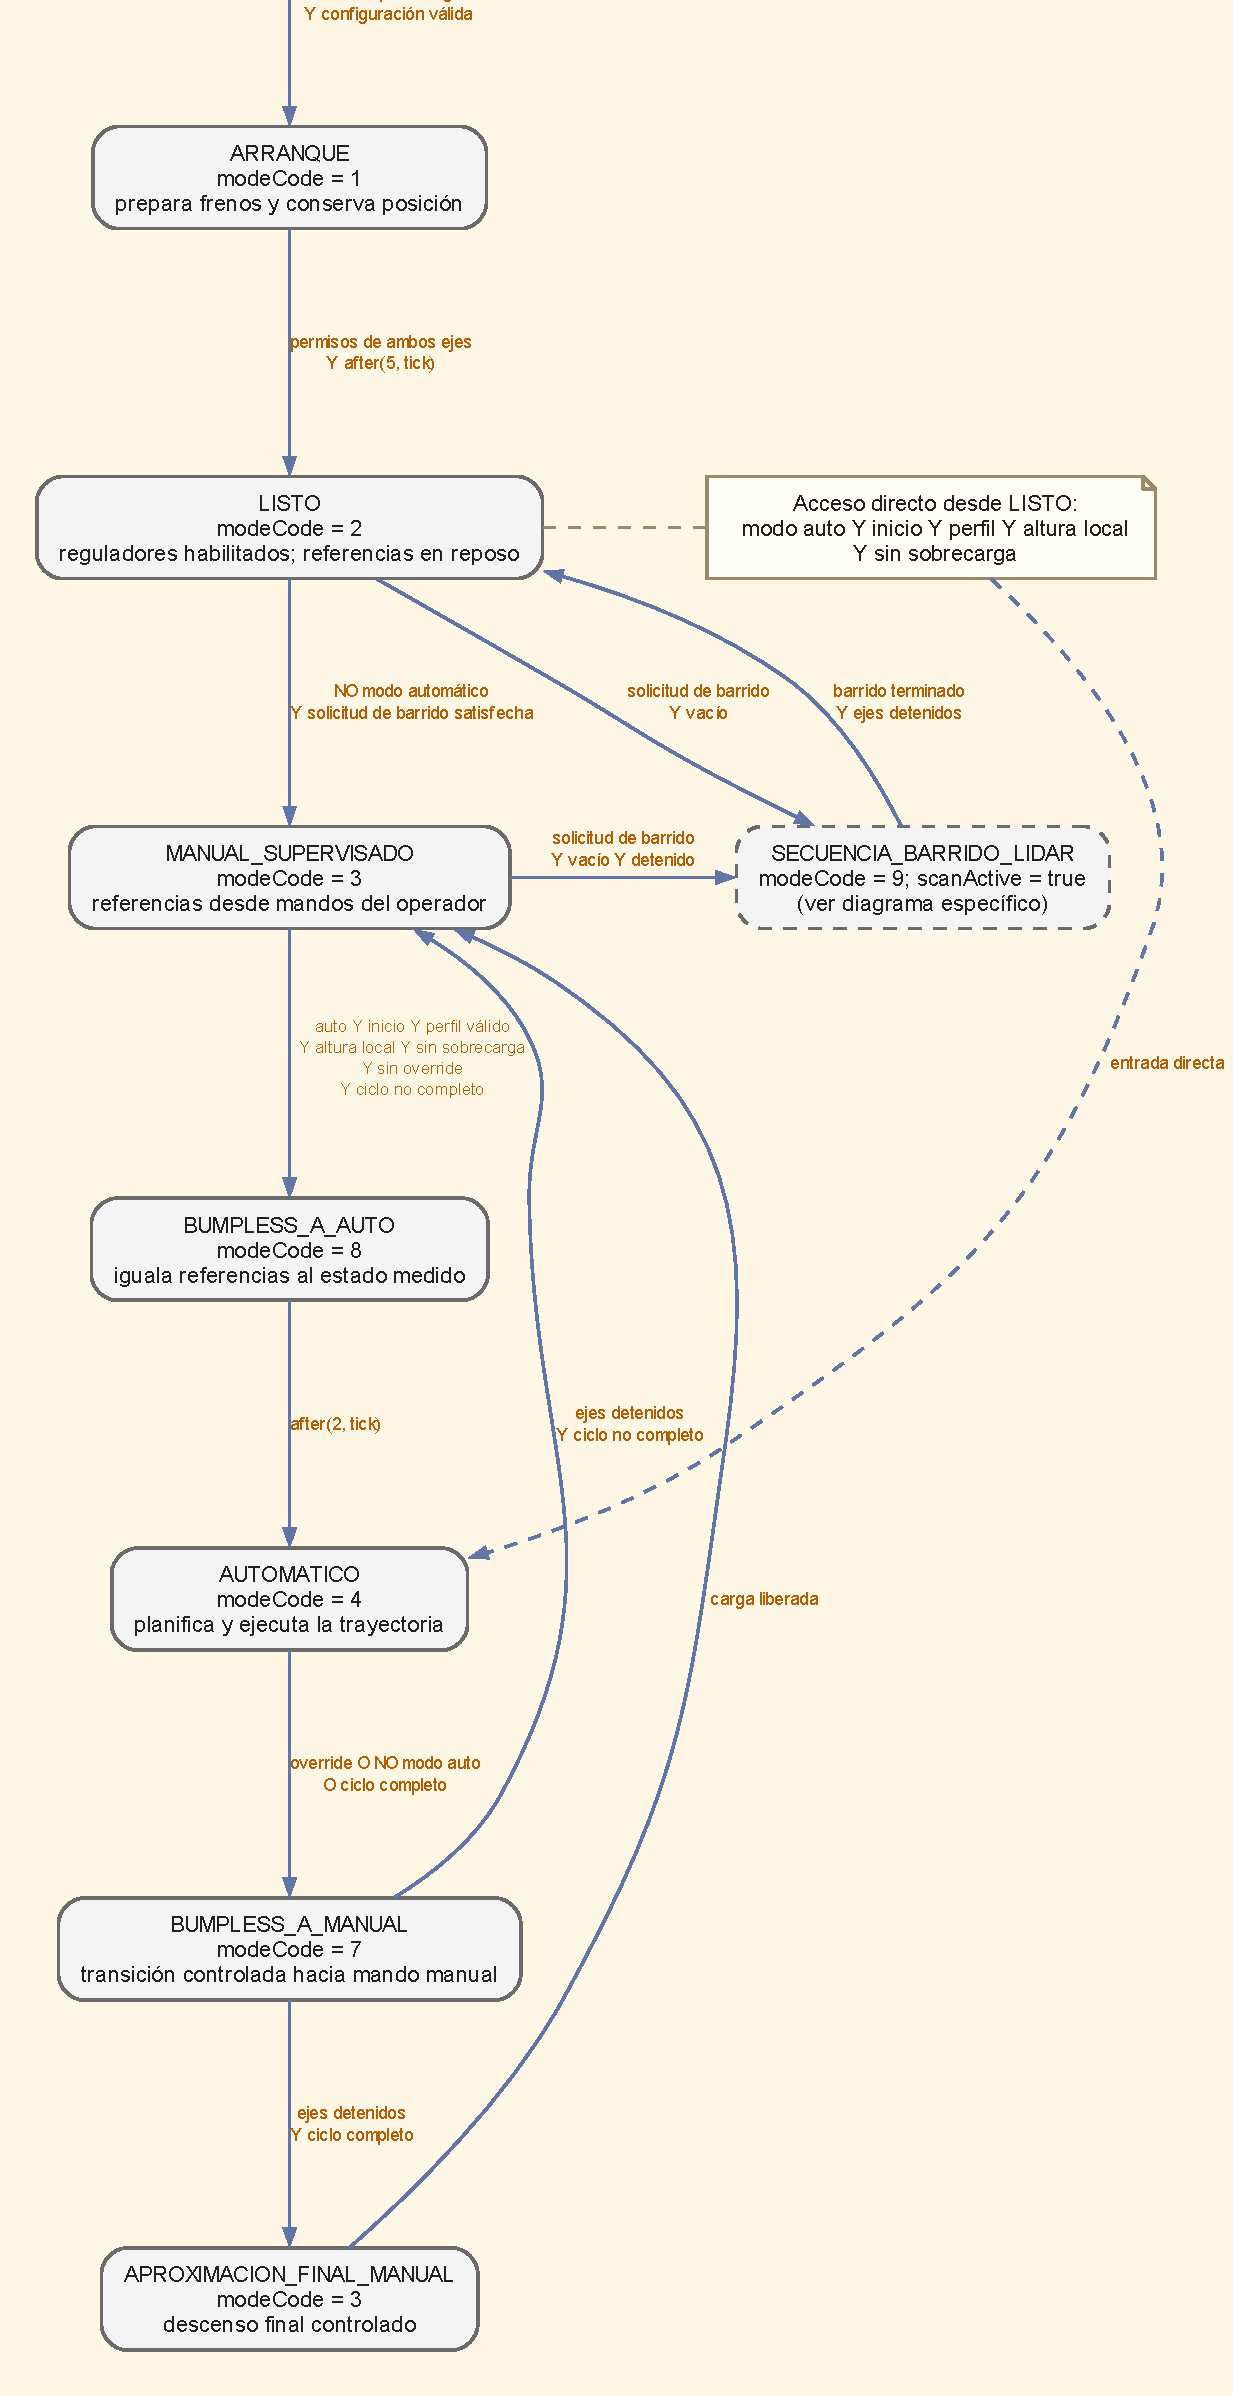
\includegraphics[height=.83\textheight,width=.98\textwidth,keepaspectratio]{imagenes_informe/otro/diagramas_automatas_revision/02b_operacion_maniobra.pdf}
\caption{Región \texttt{OPERACION}: arranque, modo manual, transferencias al modo automático y acceso al barrido. Las salidas comunes por parada y falla se muestran en la \cref{fig:supervisor_operacion_parada}.}

\label{fig:supervisor_operacion_maniobra}
\end{figure}

\Needspace{5\baselineskip}

\subsection{Estado MANUAL SUPERVISADO}
En \texttt{MANUAL\_SUPERVISADO} el código de modo es tres. Los \textit{joysticks} se convierten en velocidades con una zona muerta de $0.05$. La velocidad horizontal se limita a $4~\mathrm{m/s}$. La velocidad vertical depende del estado de carga y de la masa estimada.

Si existe sobrecarga, se anula el movimiento horizontal y solamente se permite descender con un máximo de $0.15~\mathrm{m/s}$. Los finales de carrera normales inhiben cualquier orden que intente continuar hacia afuera del recorrido. Las referencias de posición se actualizan integrando una muestra de la velocidad limitada.

Desde \texttt{MANUAL\_SUPERVISADO}, el cambio a automático exige solicitud de modo automático, orden de inicio, perfil válido, \texttt{autoEntryHeightOK}, ausencia de sobrecarga, ausencia de intervención del operador y que no exista un ciclo automático ya completado. No se exige \texttt{loadedState}, por lo que la secuencia admite traslado cargado y retorno vacío. La altura mínima se evalúa en la posición actual a partir de la envolvente local; no se utiliza \texttt{clearanceOK} como guarda.

\Needspace{5\baselineskip}

\subsection{Transferencia a automático}
El estado \texttt{BUMPLESS\_A\_AUTO} se utiliza únicamente para la transferencia desde manual y emplea el código de modo ocho. Las referencias se igualan al estado medido:
\begin{align}
x^*&=x_t,&v_x^*&=v_t,&a_x^*&=a_t,\\
y^*&=y_h,&v_y^*&=v_h,&a_y^*&=a_h.
\end{align}
Después de dos ciclos se ingresa al estado compuesto \texttt{AUTOMATICO}. Esta espera permite que los reguladores reciban una muestra coherente y evita un cambio discontinuo de torque. Existe, además, la transición directa antes mencionada desde \texttt{LISTO}; por lo tanto, no toda entrada al automático atraviesa este estado de transferencia.

Si durante la transferencia aparece una orden de parada, se va a parada normal. Si aparece una falla de seguimiento o de carga, se ingresa a retención de falla.

\Needspace{5\baselineskip}

\subsection{Subestados automáticos}
El estado \texttt{AUTOMATICO} memoriza \texttt{autoTargetX} en \texttt{autoTargetXLatched} y calcula la superficie y la altura de aproximación con \texttt{safetyEnvelopeProfile}. En cada activación posterior, \texttt{INTERLOCKS} vuelve a evaluar el objetivo vertical mediante \texttt{calcularObjetivoSeguro}; \texttt{automaticTargetY} reproduce \texttt{autoApproachTargetY}. La altura objetivo sigue la ecuación \eqref{eq:objetivo_local_vigente} y ya no se reemplaza por el máximo entre destino y línea global.

Los subestados implementados son:
\begin{itemize}
    \item \texttt{PLANIFICAR}: utiliza el código de modo cuatro, reinicia \texttt{craneTrajectoryGenerator} y obtiene el primer punto del plan coordinado.
    \item \texttt{EJECUTAR}: evalúa la trayectoria en cada ciclo, administra la habilitación anti-sway y aplica el cierre adicional de posición vertical.
    \item \texttt{MANTENER\_OBJETIVO}: fija las referencias finales y declara completo el ciclo automático.
\end{itemize}
La transición a \texttt{MANTENER\_OBJETIVO} exige solamente un error horizontal menor que $0.08~\mathrm{m}$ y un error vertical menor que $0.15~\mathrm{m}$. El generador inicia izaje y traslación simultáneamente y, si la envolvente no despeja el perfil, aumenta la duración horizontal. Utiliza el perfil dilatado, la altura del contenedor cuando hay carga, el estiramiento estimado del cable y un margen vertical de $2.59~\mathrm{m}$. La cota alta de cruce conserva además el máximo del perfil más $5.18~\mathrm{m}$. Cuando el descenso final empieza al concluir la traslación, el generador espera las condiciones de posición, velocidad y balanceo descritas en la sección de anti-sway. Durante ejecución se mantiene \texttt{swayControlEnable} según \texttt{swayControlSelect}.

\begin{figure}[!htb]
    \centering
    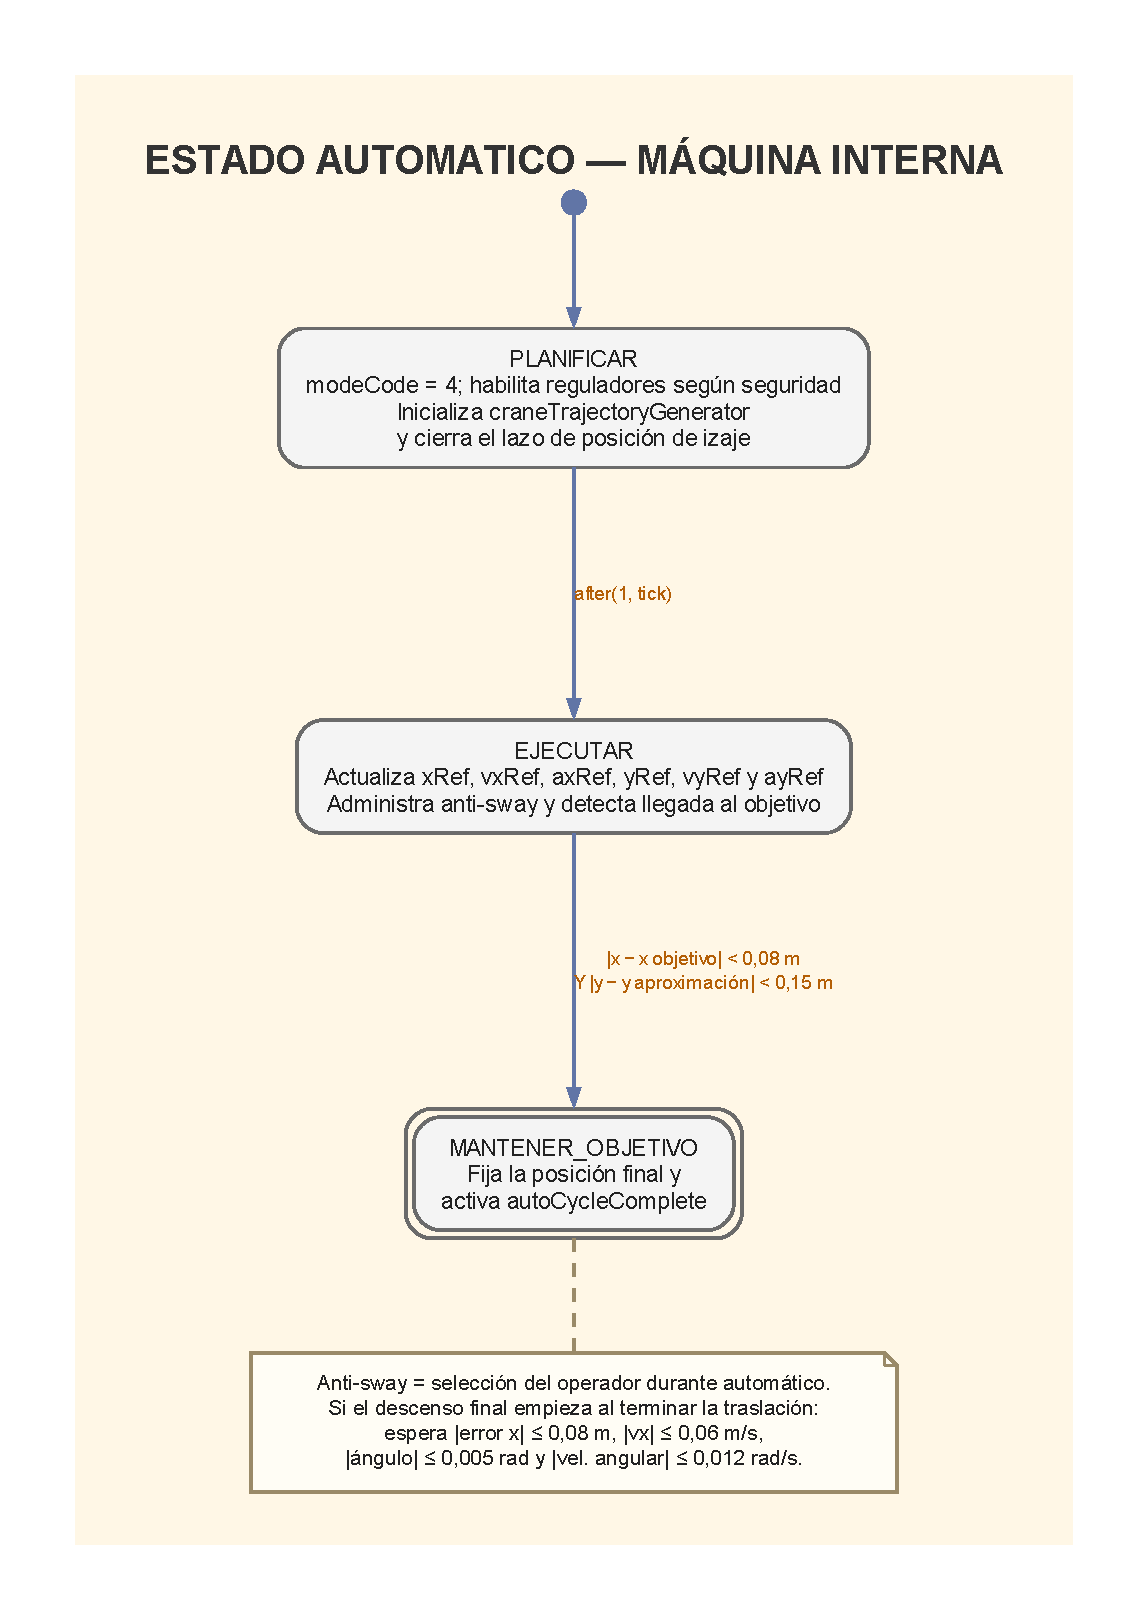
\includegraphics[height=0.75\textheight,keepaspectratio]{imagenes_informe/otro/diagramas_automatas_revision/03_automatico_interno.pdf}
    \caption{Máquina de estados interna del modo automático y acciones principales de planificación, ejecución y mantenimiento del objetivo.}
\label{fig:supervisor_automatico}
\end{figure}

\Needspace{5\baselineskip}

\subsection{Retorno a manual y aproximación final}
El automático finaliza por objetivo alcanzado, intervención del operador o cancelación del modo. Se ingresa a \path{BUMPLESS_A_MANUAL}, donde las referencias se acercan gradualmente al mando manual. Si el ciclo automático no terminó, se retorna a \path{MANUAL_SUPERVISADO}.

Cuando el objetivo fue alcanzado se pasa a \texttt{APROXIMACION\_FINAL\_MANUAL}. La posición horizontal queda fijada y el operador controla el movimiento vertical para realizar el descenso. La función limita el mando a ambos sentidos; no impone por sí sola una prohibición de ascenso. La aceleración vertical queda limitada a $0.05~\mathrm{m/s^2}$ para realizar el apoyo en forma controlada. Una vez liberado el contenedor, el autómata vuelve al modo manual general.

\Needspace{5\baselineskip}

\subsection{Parada normal y retención de falla}
\texttt{PARADA\_NORMAL} representa una detención controlada. Al ingresar se fija el código de modo cinco, se deshabilita el anti-sway y las referencias de velocidad se llevan progresivamente a cero mediante los límites de aceleración establecidos. Los reguladores permanecen disponibles durante esta reducción, por lo que la detención se diferencia de una actuación de emergencia. Una vez alcanzada la condición de reposo, el sistema retorna a \texttt{APAGADO} y requiere una nueva orden de marcha.

\texttt{RETENCION\_FALLA} se utiliza cuando aparece una falla de seguimiento, una falla de la secuencia de carga en los estados que contienen dicha transición. En este estado se deshabilita la continuidad de la maniobra y se conservan los indicadores de diagnóstico. La salida no es automática: exige orden de reinicio, permiso global restablecido y desaparición de las condiciones que originaron la retención. El destino es \texttt{APAGADO}, de modo que el rearme no produce una reanudación espontánea de la trayectoria anterior.

La emergencia se mantiene fuera de estos dos estados. Su intervención corresponde al autómata de seguridad, que actúa sobre permisos y autorizaciones de freno independientemente de la secuencia productiva.

\Needspace{5\baselineskip}

\subsection{Estados del barrido LIDAR}
La secuencia de barrido utiliza cuatro estados. \texttt{PREPARAR\_ESCANEO\_LIDAR} inicializa las 33 alturas en $-20~\mathrm{m}$, pone en cero los contadores de muestras, marca el perfil como no válido y eleva el \textit{spreader} hasta aproximadamente $39.7~\mathrm{m}$. En esta inicialización se carga de manera explícita el \textit{slot} 33 con altura cero y una muestra válida. En consecuencia, la validación posterior exige muestras efectivas en los restantes \textit{slots}, pero el último queda considerado cubierto desde el inicio.

\texttt{IR\_EXTREMO\_DERECHO} mueve el carro hasta el límite normal o hasta $x\geq48.40~\mathrm{m}$ con velocidad pequeña. \texttt{BARRIDO\_LIDAR\_IZQUIERDA} registra el máximo medido en cada \textit{slot} durante el retorno hasta el límite izquierdo o hasta $x\leq-24.50~\mathrm{m}$. \texttt{FINALIZAR\_ESCANEO\_LIDAR} detiene el carro, marca la secuencia como completa y llama a \texttt{verificarCoberturaPerfil}, que exige un contador mayor o igual que uno para cada posición.

\texttt{profileScanComplete} y \texttt{profileValid} expresan condiciones diferentes. La primera señala que terminó la secuencia de barrido; la segunda indica que el perfil fue aceptado para su utilización. Al iniciar un barrido ambas se hacen falsas. Al finalizar, \texttt{profileScanComplete} se hace verdadera y \texttt{profileValid} recibe el resultado de la comprobación de cobertura de los 33 \textit{slots}; por tanto, el barrido puede terminar sin obtener un perfil válido. En el banco de medio ciclo, la precarga permite un perfil válido con \texttt{profileScanComplete=false}, porque no se realizó un relevamiento. Además, cuando no hay solicitud ni barrido activo, el supervisor limpia la bandera de finalización sin invalidar por esa operación el perfil conservado. La finalización no constituye un certificado permanente de procedencia y la validez no implica que el barrido se haya ejecutado en ese ensayo.

El barrido no puede iniciarse con carga. Durante los cuatro estados se atiende la orden de parada y la pérdida del permiso global. Las transiciones específicas hacia \texttt{RETENCION\_FALLA} comprueban \texttt{loadSequenceFault}, pero no incluyen \texttt{trackingFault}.

\begin{figure}[H]
\centering
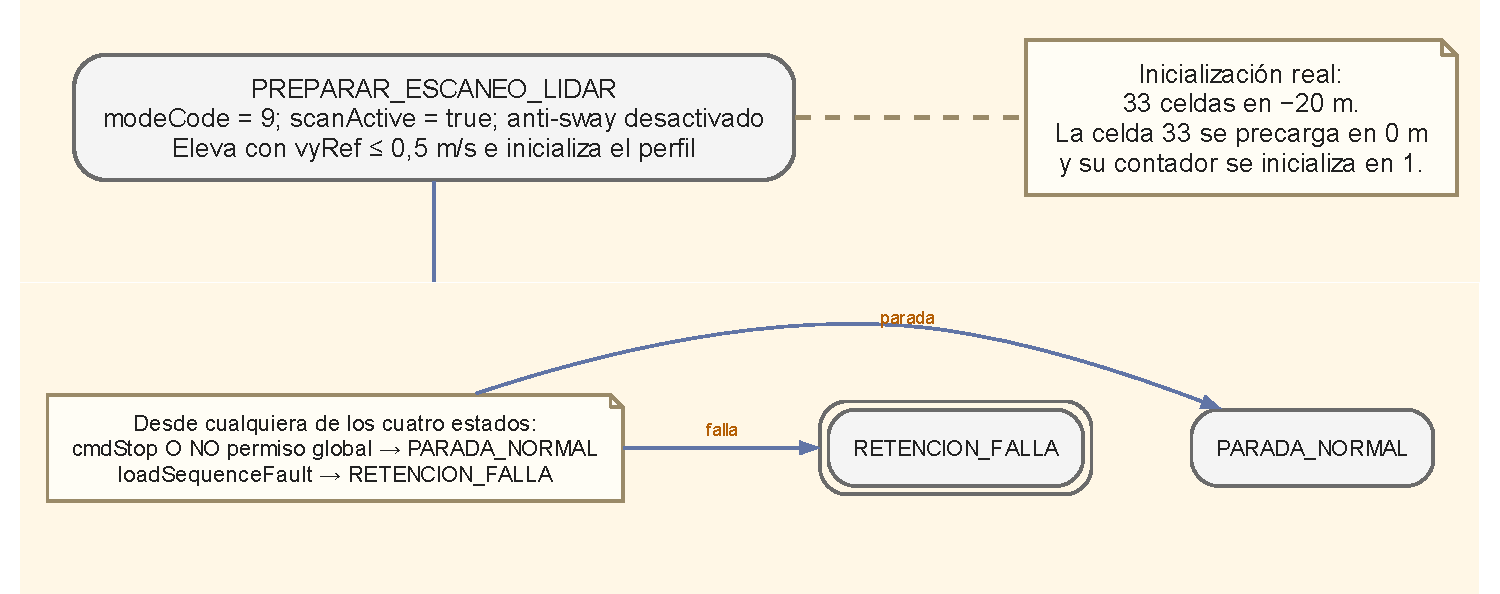
\includegraphics[width=.98\textwidth,clip]{imagenes_informe/otro/diagramas_automatas_revision/04a_barrido_preparacion.pdf}
\caption{Relevamiento LiDAR: preparación e inicialización del perfil y salidas comunes por parada o falla. La condición de altura y velocidad habilita el recorrido de la \cref{fig:supervisor_barrido_recorrido}.}

\label{fig:supervisor_barrido_preparacion}
\end{figure}

\begin{figure}[H]
\centering
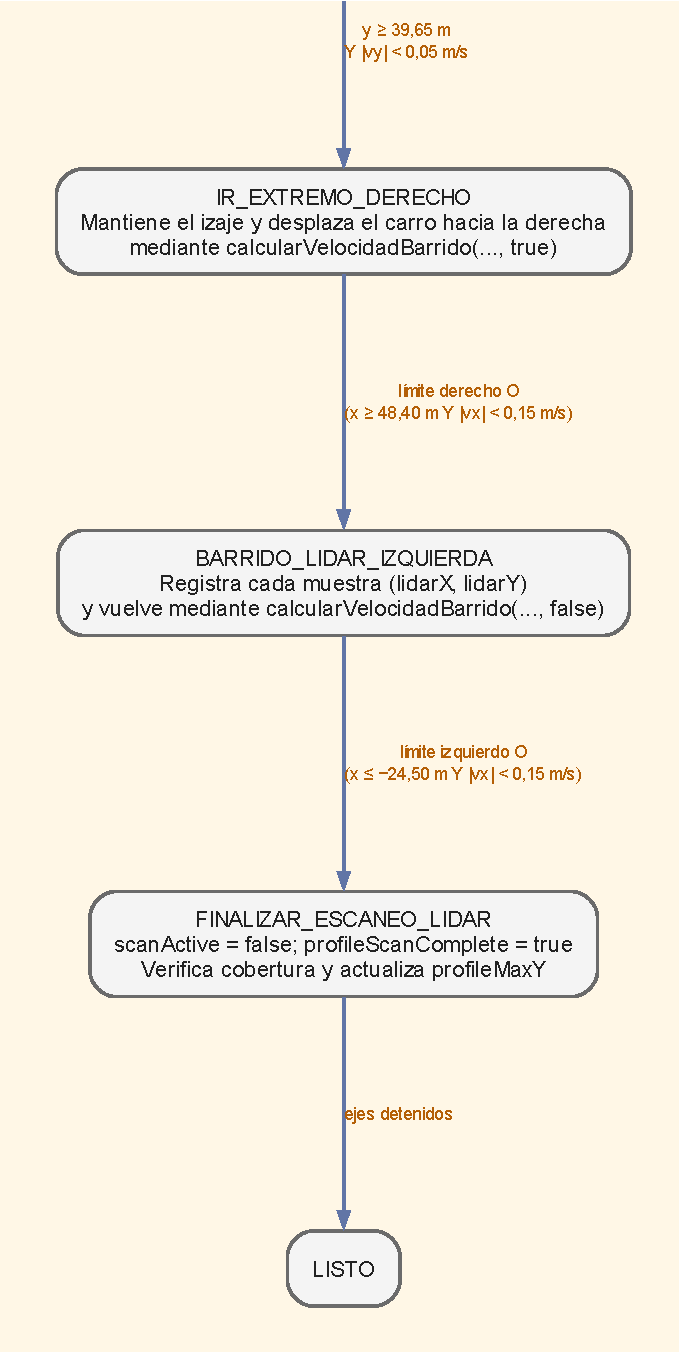
\includegraphics[height=.50\textheight,width=.98\textwidth,keepaspectratio]{imagenes_informe/otro/diagramas_automatas_revision/04b_barrido_recorrido.pdf}
\caption{Relevamiento LiDAR: aproximación al extremo derecho, barrido hacia la izquierda, validación de cobertura y retorno a \texttt{LISTO}. Las salidas comunes por parada y falla se muestran en la \cref{fig:supervisor_barrido_preparacion}.}

\label{fig:supervisor_barrido_recorrido}
\end{figure}

\Needspace{5\baselineskip}

\subsection{Secuencia de toma y estabilización}
La región de carga comienza en \texttt{VACIO}. Ante una solicitud de cierre, contacto en los cuatro apoyos y permiso de izaje, pasa a \texttt{ESPERAR\_ESTABILIZACION\_SPREADER}. Se exige durante un segundo
\begin{equation}
|\theta_l|\leq0.010~\mathrm{rad},\qquad |\dot\theta_l|\leq0.020~\mathrm{rad/s}.
\end{equation}
Luego se ingresa a \path{CERRANDO_TWISTLOCKS}. Si la confirmación no aparece antes de 100 ciclos se declara \path{FALLA_TWISTLOCK}. Al confirmarse el cierre se ingresa a \path{DESPEGUE_SUAVE}, donde se activa \texttt{loadedState} y \texttt{pickupModeActive}, sin habilitar todavía la estimación de masa.

Mientras el contenedor continúa apoyado y no se completó una segunda comprobación de estabilidad posterior al cierre, \texttt{aplicarRetencionToma} fuerza a cero las referencias manuales horizontal y vertical. El estado \path{DESPEGUE_SUAVE} no contiene una rampa ni un límite de velocidad propios; una vez liberada esta retención se aplican los límites generales del mando manual cargado. Antes de completar el pesaje, \texttt{totalSuspendedMass} conserva el valor inicial de $15000~\mathrm{kg}$ y el cálculo manual puede admitir hasta $3~\mathrm{m/s}$.

\Needspace{5\baselineskip}

\subsection{Pesaje y sobrecarga}
Cuando el cable deja de estar flojo, $|v_h|<0.20~\mathrm{m/s}$ y $|a_h|<0.05~\mathrm{m/s^2}$, se ingresa a \texttt{PESAJE}. Durante 25 ciclos se acumulan muestras de masa estimada. El promedio reduce el efecto de oscilaciones de tensión.

Cada muestra se obtiene a partir de la tensión medida por ramal $F_{hw,\mathrm{sens}}[n]$ y de la confirmación de \textit{twistlocks} cerrados $c_{\mathrm{TL}}[n]$. La estimación instantánea de la masa del contenedor implementada en el código es
\begin{equation}
\boxed{
\widehat M_c^{\,\mathrm{inst}}[n]=
\begin{cases}
\displaystyle\max\left(0,\frac{2F_{hw,\mathrm{sens}}[n]}{g}-M_s\right),
& c_{\mathrm{TL}}[n]=1,\\[6pt]
0, & c_{\mathrm{TL}}[n]=0,
\end{cases}}
\end{equation}
con $g=9{,}80665~\mathrm{m/s^2}$ y $M_s=15000~\mathrm{kg}$. El factor 2 corresponde a los dos ramales que sostienen el conjunto. Se resta la masa del \textit{spreader} para obtener la del contenedor, y el máximo con cero evita estimaciones negativas. Estas estimaciones instantáneas son las muestras que se promedian durante el pesaje.

Si la masa estimada del contenedor no supera $50000~\mathrm{kg}$ se pasa a \texttt{CARGADO}. Si supera ese límite se pasa a \texttt{SOBRECARGA}. En sobrecarga no se permite el traslado y solamente puede ordenarse una descarga controlada.

La apertura de \textit{twistlocks} se permite con contacto. El estado \texttt{ABRIENDO\_TWISTLOCKS} espera la confirmación de apertura y retorna a \texttt{VACIO}. También dispone de un tiempo máximo de 100 ciclos.

\begin{figure}[!htb]
    \centering
    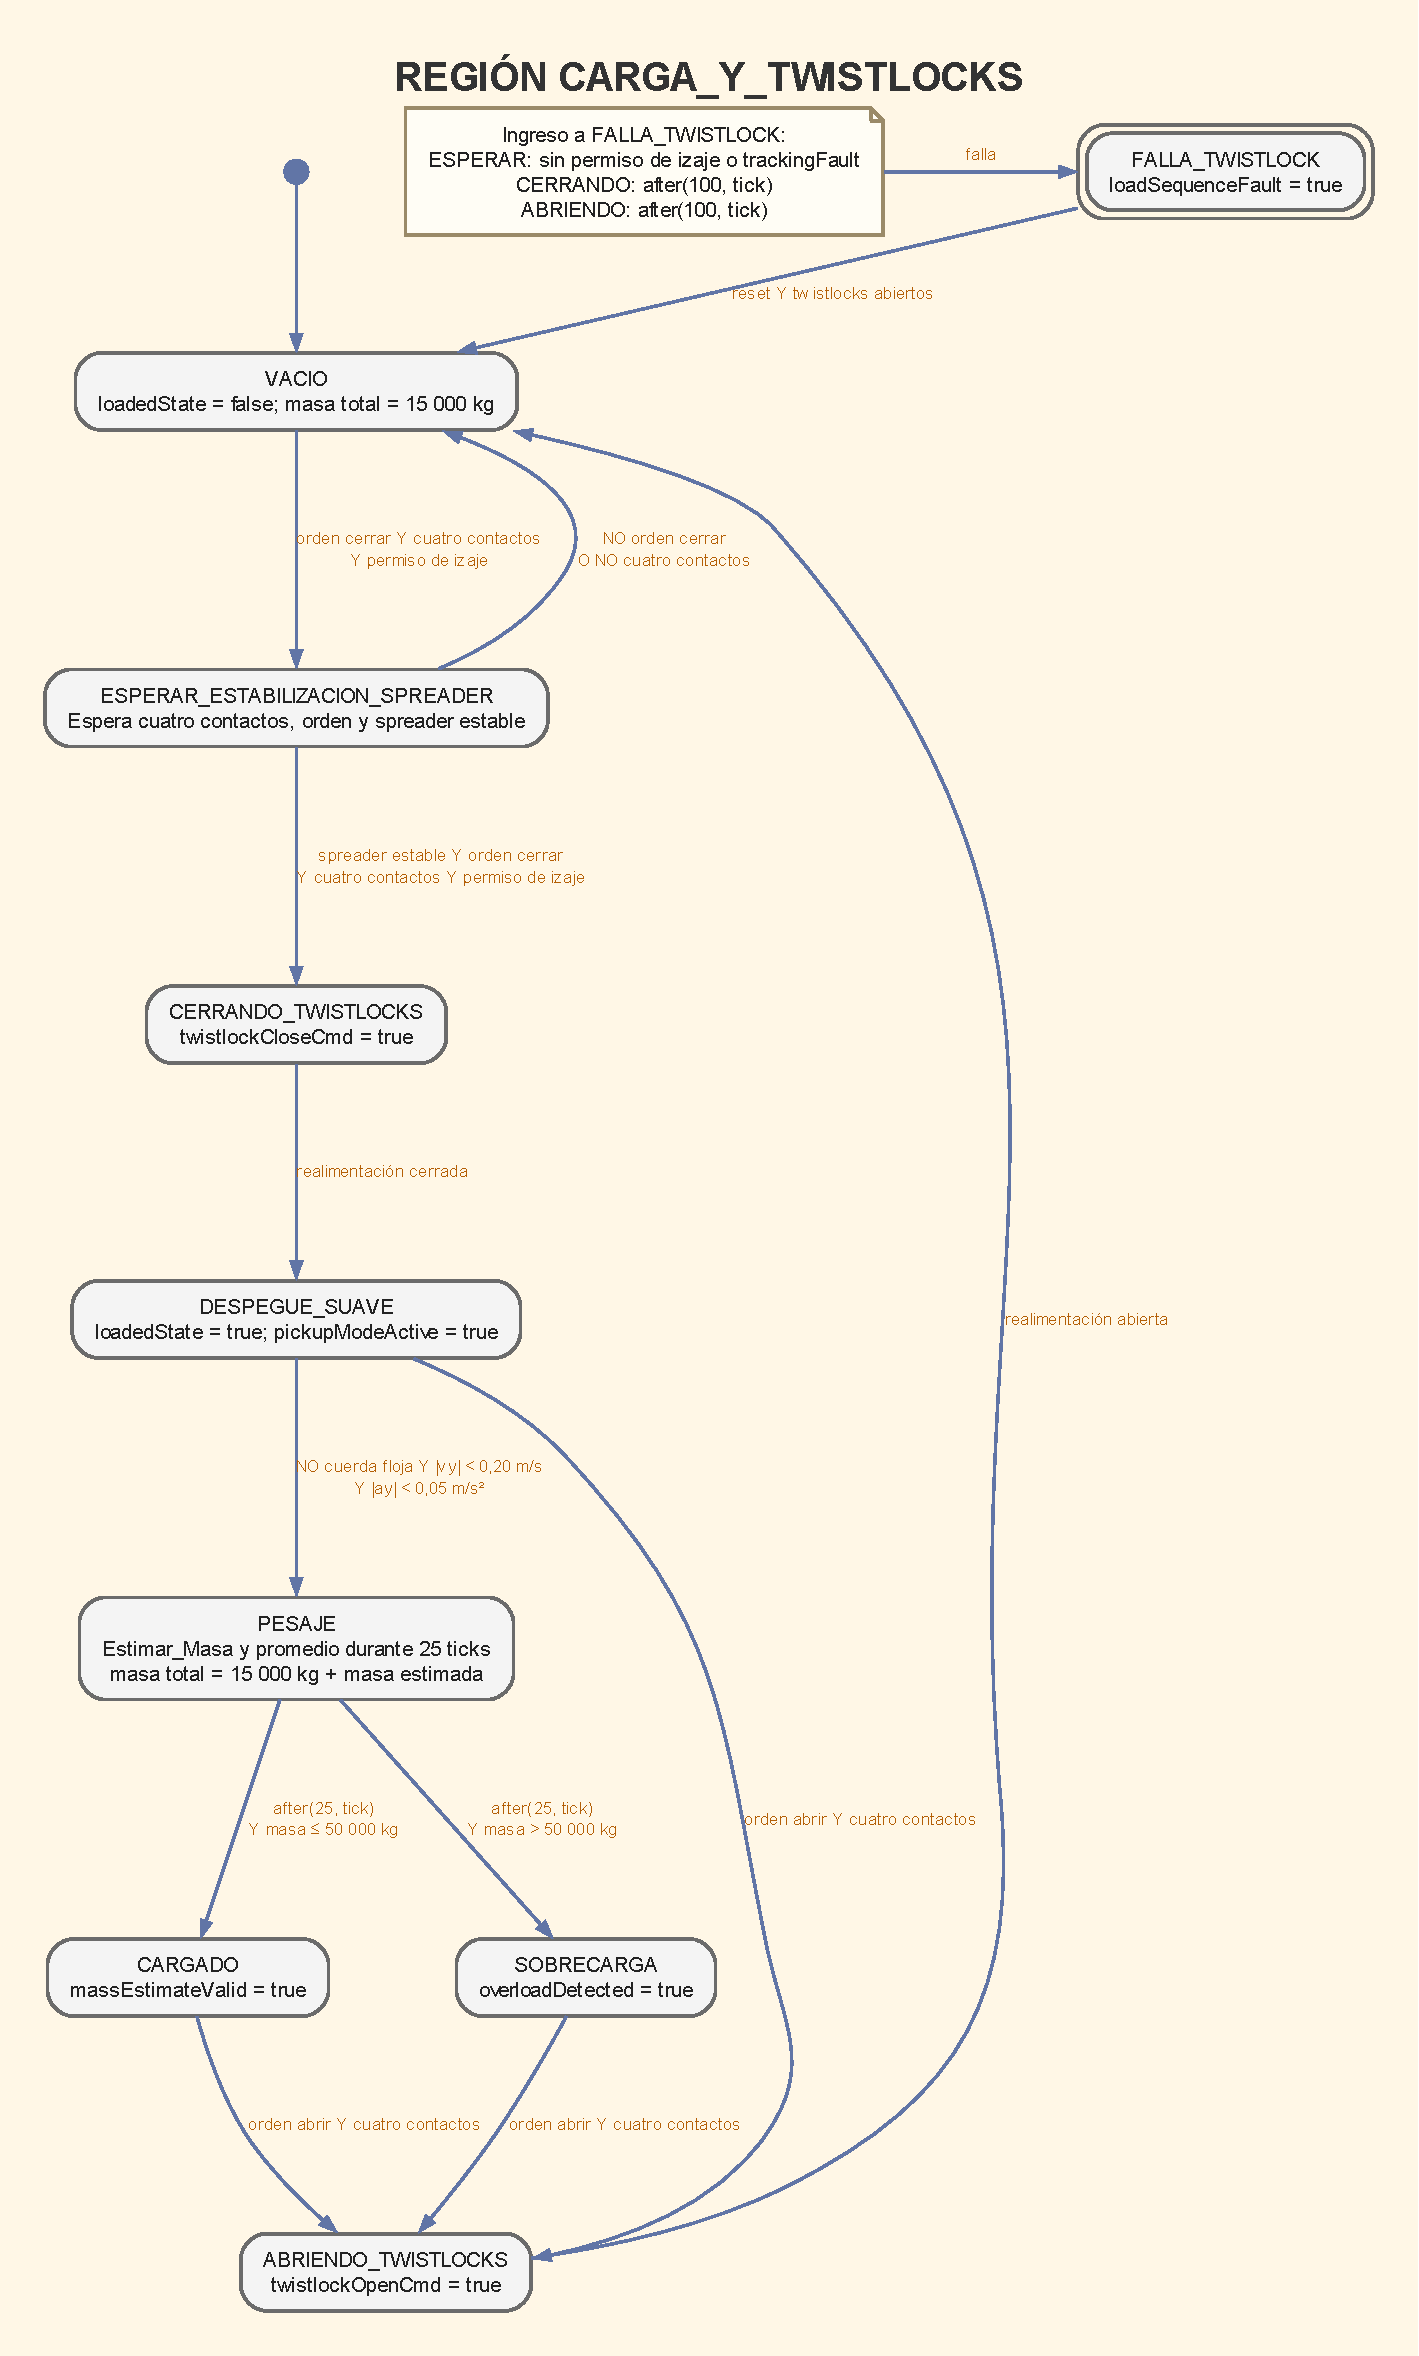
\includegraphics[width=.98\textwidth,height=.88\textheight,keepaspectratio]{imagenes_informe/otro/diagramas_automatas_revision/05_carga_twistlocks_recortado.pdf}
    \caption{Máquina de estados completa de la región \texttt{CARGA\_Y\_TWISTLOCKS}, desde la toma hasta la liberación o retención por falla.}
\label{fig:supervisor_carga}
\end{figure}

\Needspace{5\baselineskip}

\clearpage
\subsection{Indexación de estados de carga}
\begin{table}[H]
\centering
\caption{Índice funcional de la región de carga.}
\begin{tabular}{C{1.2cm} L{5cm} L{7.2cm}}
\toprule
Índice & Estado & Acción principal\\
\midrule
C0 & \texttt{VACIO} & Reinicia masa, carga y comandos de cierre.\\
C1 & \path{ESPERAR_ESTABILIZACION_SPREADER} & Verifica ángulo y velocidad angular.\\
C2 & \texttt{CERRANDO\_TWISTLOCKS} & Comanda cierre y temporiza confirmación.\\
C3 & \texttt{DESPEGUE\_SUAVE} & Declara carga tomada y retiene el mando hasta la segunda estabilidad; no impone una velocidad propia.\\
C4 & \texttt{PESAJE} & Promedia la masa estimada durante 25 ciclos.\\
C5 & \texttt{CARGADO} & Habilita traslado normal.\\
C6 & \texttt{SOBRECARGA} & Inhibe traslado y limita el descenso.\\
C7 & \texttt{ABRIENDO\_TWISTLOCKS} & Comanda apertura y espera realimentación.\\
C8 & \texttt{FALLA\_TWISTLOCK} & Retiene comandos hasta reinicio seguro.\\
\bottomrule
\end{tabular}
\end{table}



\Needspace{5\baselineskip}

\subsection{Secuencia del freno de izaje}
La región \texttt{FRENO\_IZAJE} posee cuatro estados:
\begin{itemize}
    \item H0 -- \texttt{HB\_APLICADO}: freno cerrado.
    \item H1 -- \texttt{HB\_PRUEBA\_TORQUE}: el regulador establece torque con freno aplicado.
    \item H2 -- \texttt{HB\_ABIERTO}: freno liberado durante el movimiento.
    \item H3 -- \texttt{HB\_APLICANDO}: mantiene apertura hasta que velocidad y error son pequeños.
\end{itemize}
Desde H1 se vuelve a H0 si no se demuestra torque antes de 50 ciclos. Desde H2 se pasa a H3 si falta habilitación o permiso de izaje; la ausencia de demanda sólo provoca esta transición cuando \texttt{modeCode} es distinto de cuatro. Así se mantiene el freno operativo abierto durante el automático aun si momentáneamente la referencia de velocidad y el error son pequeños. La apertura solamente se produce con \path{torqueProvenHoist}. Al terminar el movimiento, el freno se aplica cuando $|v_h|<0.03~\mathrm{m/s}$ y el error vertical es menor o igual que $0.05~\mathrm{m}$.

\Needspace{5\baselineskip}

\subsection{Secuencia del freno del carro}
La región \texttt{FRENO\_CARRO} reproduce la misma filosofía:
\begin{itemize}
    \item T0 -- \texttt{TB\_APLICADO}.
    \item T1 -- \texttt{TB\_PRUEBA\_TORQUE}.
    \item T2 -- \texttt{TB\_ABIERTO}.
    \item T3 -- \texttt{TB\_APLICANDO}.
\end{itemize}
La prueba comienza si el regulador está habilitado, existe una referencia de movimiento y el permiso de seguridad del carro está activo. La aplicación final exige $|v_t|<0.03~\mathrm{m/s}$ y error de posición menor o igual que $0.03~\mathrm{m}$.

Estas máquinas impiden liberar un freno por la sola presencia de una orden de movimiento. La confirmación de torque proporciona una condición adicional antes de dejar el eje libre.

La indexación consolidada de ambas regiones se presenta en la \cref{tab:indices_frenos}. La letra identifica el eje y permite conservar el mismo número para estados de función equivalente.

\begin{table}[!htb]
\centering
\caption{Índice y acciones de los estados de freno.}\label{tab:indices_frenos}
\begin{tabular}{C{1.1cm} L{4.3cm} L{8.0cm}}
\toprule
Índice & Estado & Acción documentada\\
\midrule
H0 & \texttt{HB\_APLICADO} & Mantiene aplicado el freno de izaje.\\
H1 & \texttt{HB\_PRUEBA\_TORQUE} & Solicita torque y espera su comprobación.\\
H2 & \texttt{HB\_ABIERTO} & Autoriza la apertura durante el movimiento vertical.\\
H3 & \texttt{HB\_APLICANDO} & Espera reposo y completa la aplicación del freno.\\
T0 & \texttt{TB\_APLICADO} & Mantiene aplicado el freno del carro.\\
T1 & \texttt{TB\_PRUEBA\_TORQUE} & Solicita torque y espera su comprobación.\\
T2 & \texttt{TB\_ABIERTO} & Autoriza la apertura durante el movimiento horizontal.\\
T3 & \texttt{TB\_APLICANDO} & Espera reposo y completa la aplicación del freno.\\
\bottomrule
\end{tabular}
\end{table}

\begin{figure}[!htb]
    \centering
    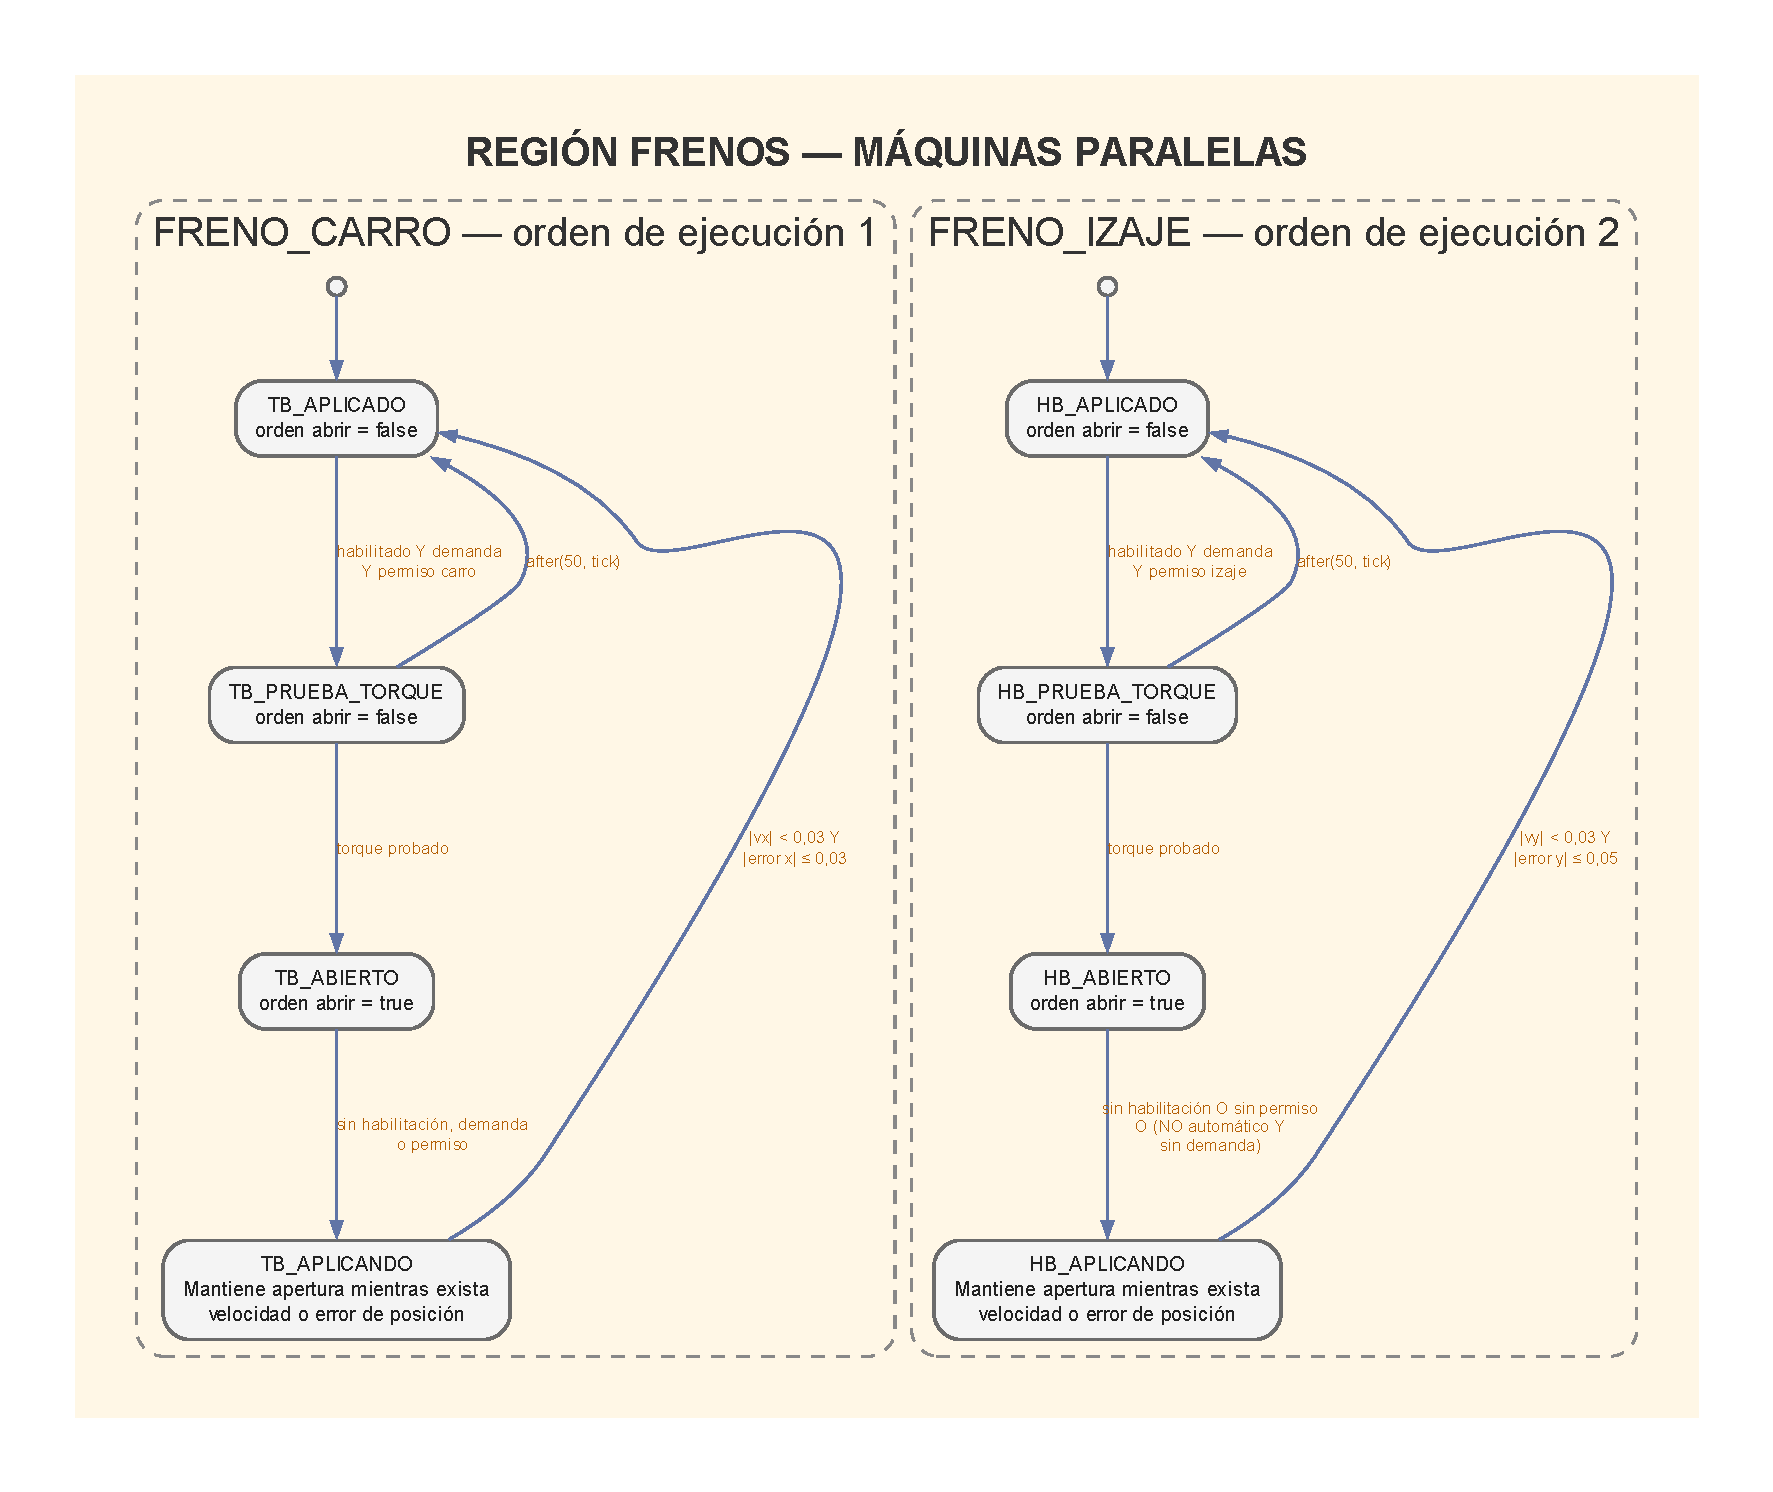
\includegraphics[width=0.94\textwidth,height=0.68\textheight,keepaspectratio]{imagenes_informe/otro/diagramas_automatas_revision/06_frenos.pdf}
    \caption{Máquinas paralelas de accionamiento de los frenos del carro y del izaje.}
\label{fig:supervisor_frenos}
\end{figure}

\Needspace{5\baselineskip}

\subsection{Diagnóstico del supervisor}
La región \texttt{DIAGNOSTICO} contiene \texttt{DIAG\_OK}, \texttt{ALARMA} y \texttt{FALLA}. La sobrecarga produce una alarma recuperable. Una falla de seguimiento, una falla de secuencia de carga o la pérdida del permiso global produce una falla.

Los códigos implementados son:
\begin{itemize}
    \item código de alarma 1: sobrecarga;
    \item código de falla 10: error de seguimiento sostenido;
    \item código de falla 11: falla de secuencia de carga;
    \item código de falla 12: permiso global de seguridad ausente.
\end{itemize}
La falla de seguimiento se activa en los modos cuatro u ocho si $|x^*-x_t|>2.5~\mathrm{m}$ o $|y^*-y_h|>\max(1.00,2|v_h|+0.25)~\mathrm{m}$ se mantiene durante al menos tres segundos. En los demás modos se reinicia el temporizador.

\begin{table}[!htb]
\centering
\caption{Índice funcional de la región de diagnóstico.}\label{tab:indice_diagnostico}
\begin{tabular}{C{1.2cm} L{3.5cm} L{8.7cm}}
\toprule
Índice & Estado & Función\\
\midrule
D0 & \texttt{DIAG\_OK} & Mantiene códigos de alarma y falla sin condición activa.\\
D1 & \texttt{ALARMA} & Informa sobrecarga recuperable mediante el código de alarma 1.\\
D2 & \texttt{FALLA} & Conserva el código correspondiente a seguimiento, carga o permiso global.\\
\bottomrule
\end{tabular}
\end{table}

\begin{figure}[!htb]
    \centering
    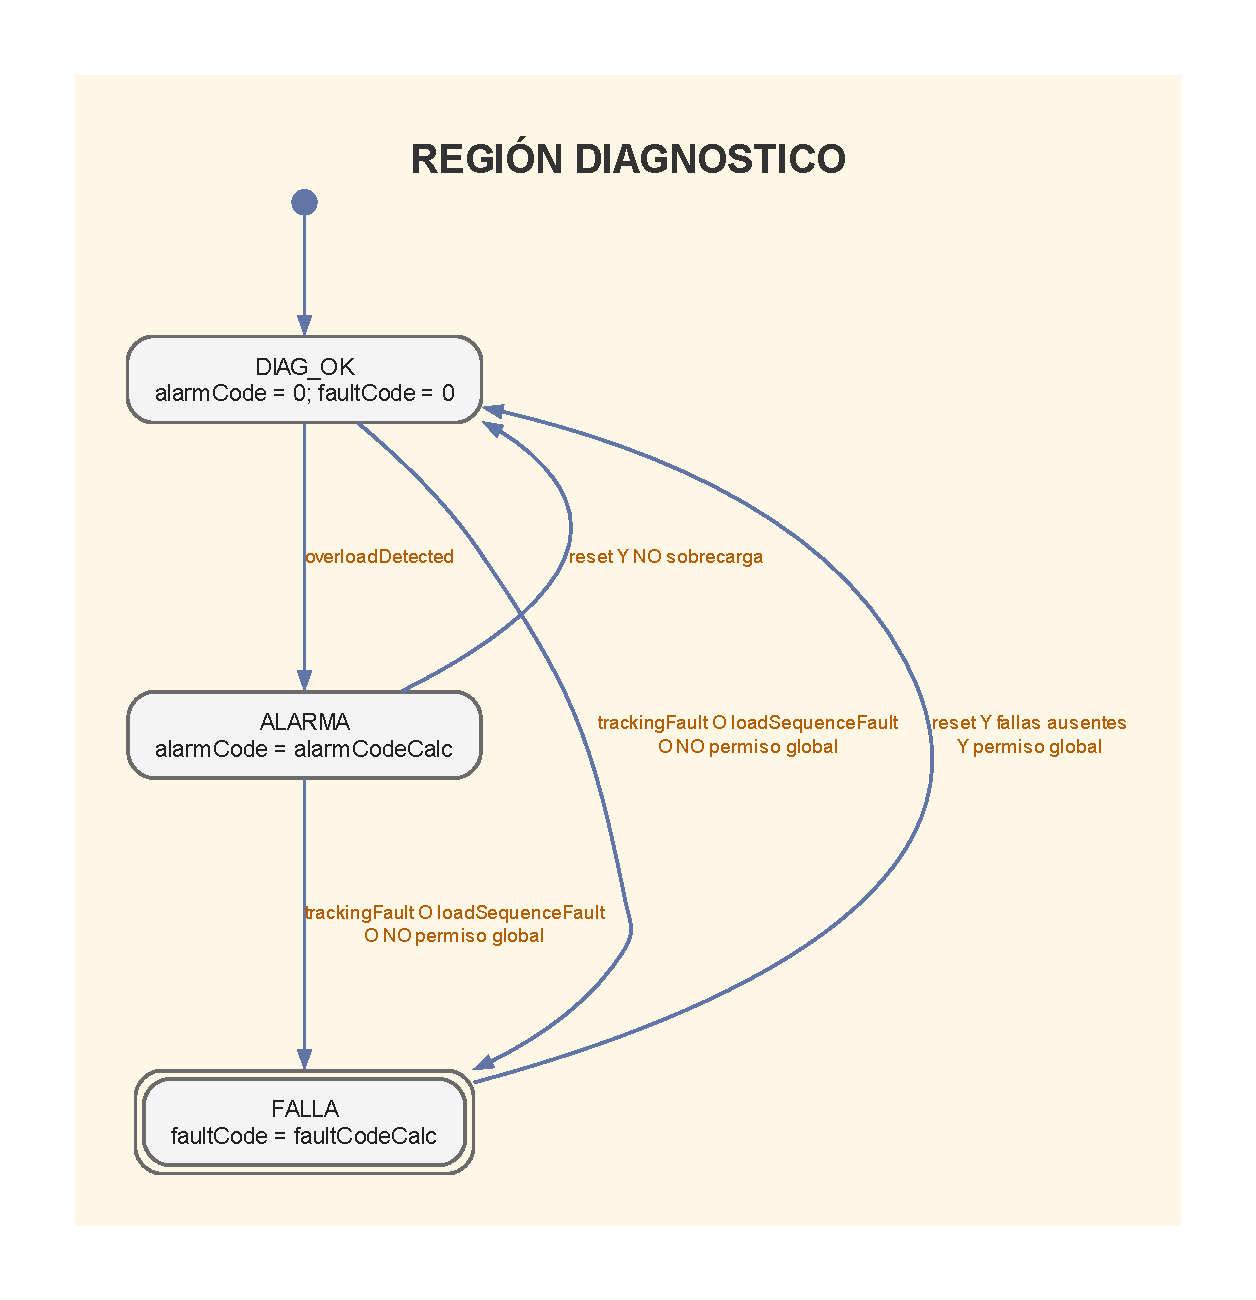
\includegraphics[height=0.68\textheight,keepaspectratio]{imagenes_informe/otro/diagramas_automatas_revision/07_diagnostico.pdf}
    \caption{Región de diagnóstico del supervisor y condiciones de generación y recuperación de alarmas y fallas.}
\label{fig:supervisor_diagnostico}
\end{figure}

\Needspace{8\baselineskip}

\subsection{Transiciones y prioridades de operación}

La prioridad entre condiciones simultáneas depende del orden de las transiciones salientes de cada estado. En manual y automático, algunas transiciones normales se evalúan antes que las de parada o falla; por ello, si coinciden, la atención de estas últimas puede desplazarse a la activación siguiente. La \cref{tab:transiciones_operacion} reúne las guardas de las transiciones principales y su prioridad relativa cuando más de una condición resulta verdadera en la misma activación.

{\footnotesize
\Needspace{12\baselineskip}
\begin{longtable}{L{3.5cm} L{3.5cm} L{6.4cm} C{1.0cm}}
\caption{Transiciones principales de la región \texttt{OPERACION}.}\label{tab:transiciones_operacion}\\
\toprule
Origen & Destino & Condición funcional resumida & Orden\\
\midrule
\endfirsthead
\toprule
Origen & Destino & Condición funcional resumida & Orden\\
\midrule
\endhead
\texttt{APAGADO} & \texttt{ARRANQUE} & Marcha, permiso global y configuración válida & 1\\
\texttt{ARRANQUE} & \texttt{LISTO} & Cinco ciclos con permisos de ambos ejes & 1\\
\texttt{LISTO} & \texttt{MANUAL\_SUPERVISADO} & Modo manual y solicitud de barrido ausente o satisfecha & 1\\
\texttt{LISTO} & \texttt{AUTOMATICO} & Modo e inicio automático, perfil válido, altura local y sin sobrecarga & 2\\
\texttt{LISTO} & \path{PREPARAR_ESCANEO_LIDAR} & Escaneo pendiente, no completado y conjunto vacío & 5\\
\path{MANUAL_SUPERVISADO} & \path{BUMPLESS_A_AUTO} & Inicio automático, perfil y altura local válidos, sin sobrecarga ni intervención, ciclo no completo & 1\\
\path{MANUAL_SUPERVISADO} & \texttt{PARADA\_NORMAL} & Orden de parada o pérdida de permiso & 2\\
\path{MANUAL_SUPERVISADO} & \texttt{RETENCION\_FALLA} & Falla de seguimiento o de carga & 3\\
\path{BUMPLESS_A_AUTO} & \texttt{AUTOMATICO} & Dos ciclos de inicialización cumplidos & 1\\
\texttt{AUTOMATICO} & \path{BUMPLESS_A_MANUAL} & Objetivo, intervención manual o cancelación & 1\\
\texttt{AUTOMATICO} & \texttt{PARADA\_NORMAL} & Orden de parada o pérdida de permiso & 2\\
\texttt{AUTOMATICO} & \texttt{RETENCION\_FALLA} & Falla de seguimiento o de carga & 3\\
\path{BUMPLESS_A_MANUAL} & \path{APROXIMACION_FINAL_MANUAL} & $|v_t|<0.10$, $|v_h|<0.03$ y ciclo completado & 4\\
\path{BUMPLESS_A_MANUAL} & \path{MANUAL_SUPERVISADO} & $|v_t|<0.10$, $|v_h|<0.03$ y ciclo no completado & 1\\
\path{APROXIMACION_FINAL_MANUAL} & \path{MANUAL_SUPERVISADO} & Contenedor liberado & 1\\
\path{FINALIZAR_ESCANEO_LIDAR} & \texttt{LISTO} & Ejes detenidos; no exige \texttt{profileValid} & 1\\
\texttt{RETENCION\_FALLA} & \texttt{APAGADO} & Reinicio, permiso global y causas eliminadas & 1\\
\bottomrule
\end{longtable}
}

\Needspace{5\baselineskip}

\par
\Needspace{10\baselineskip}
\section{Autómata de seguridad}
\label{sec:seguridad_MIL}
El diseño del nivel de seguridad y su realización en Stateflow se describen aquí. La traducción y generación de código para CODESYS se presentan en la sección~\ref{sec:implementacion_codesys}.

\Needspace{5\baselineskip}

\subsection{Correspondencia con el modelo vigente}
La revisión del chart de protección confirma la misma estructura de dos regiones paralelas, cuatro estados de emergencia y dos estados de watchdog. Se mantienen las guardas por flanco, las polaridades de autorización de freno y el orden de ejecución. Por ello, los diagramas de emergencias y watchdog conservan su topología. Se explicitan aquí las prioridades y los tiempos para que esta sección corresponda con la misma referencia que el supervisor.

\Needspace{5\baselineskip}

\subsection{Criterio de independencia}
El nivel de seguridad se encuentra en un subsistema separado y no depende del estado interno del supervisor para detectar una condición peligrosa. Recibe directamente el pulsador de emergencia, los límites últimos, el exceso de velocidad vertical, el pulso de \textit{watchdog} y la orden de reinicio.

El chart \texttt{Automata de proteccion} entrega las señales \texttt{BRK\_t}, \texttt{BRK\_h}, \texttt{BRK\_hE}, \texttt{EMERGENCIA} y \path{PARADA_EMERGENCIA_WD}. Fuera del chart, el subsistema convierte las tres primeras señales en permisos y órdenes de apertura de freno de acuerdo con
\begin{align}
\texttt{permitTrolley}&=\texttt{BRK\_t},\\
\texttt{permitHoist}&=\texttt{BRK\_h},\\
\texttt{permitGlobal}&=\texttt{BRK\_t}\ \mathrm{OR}\ \texttt{BRK\_h}.
\end{align}
Las órdenes normales del supervisor se combinan posteriormente con estas autorizaciones, de modo que no pueden abrir un freno prohibido por el nivel de seguridad.

\begin{table}[!htb]
\centering
\caption{Polaridad y significado de las salidas principales de seguridad.}\label{tab:polaridad_seguridad}
\begin{tabular}{L{3.4cm} C{2.0cm} C{2.0cm} L{6.2cm}}
\toprule
Señal & Normal & Intervención & Interpretación\\
\midrule
\texttt{BRK\_t} & 1 & 0 & Autorización para liberar el freno del carro.\\
\texttt{BRK\_h} & 1 & 0 & Autorización para liberar el freno operativo de izaje.\\
\texttt{BRK\_hE} & 1 & 0 & Autorización para liberar el freno de emergencia de izaje.\\
\texttt{EMERGENCIA} & 0 & 1 & Indicación general de una emergencia activa.\\
\path{PARADA_EMERGENCIA_WD} & 0 & 1 & Solicitud de emergencia total originada por el watchdog.\\
\bottomrule
\end{tabular}
\end{table}

Las salidas \texttt{BRK\_t}, \texttt{BRK\_h} y \texttt{BRK\_hE} son autorizaciones de apertura activas en uno. Su valor cero exige aplicar el freno correspondiente. En esta implementación, el permiso global se obtiene mediante OR de las autorizaciones de carro e izaje; por tanto, una emergencia parcial inhibe el eje afectado y conserva autorizado el otro, mientras que una emergencia total anula ambos permisos.

\begin{figure}[!htb]
\centering
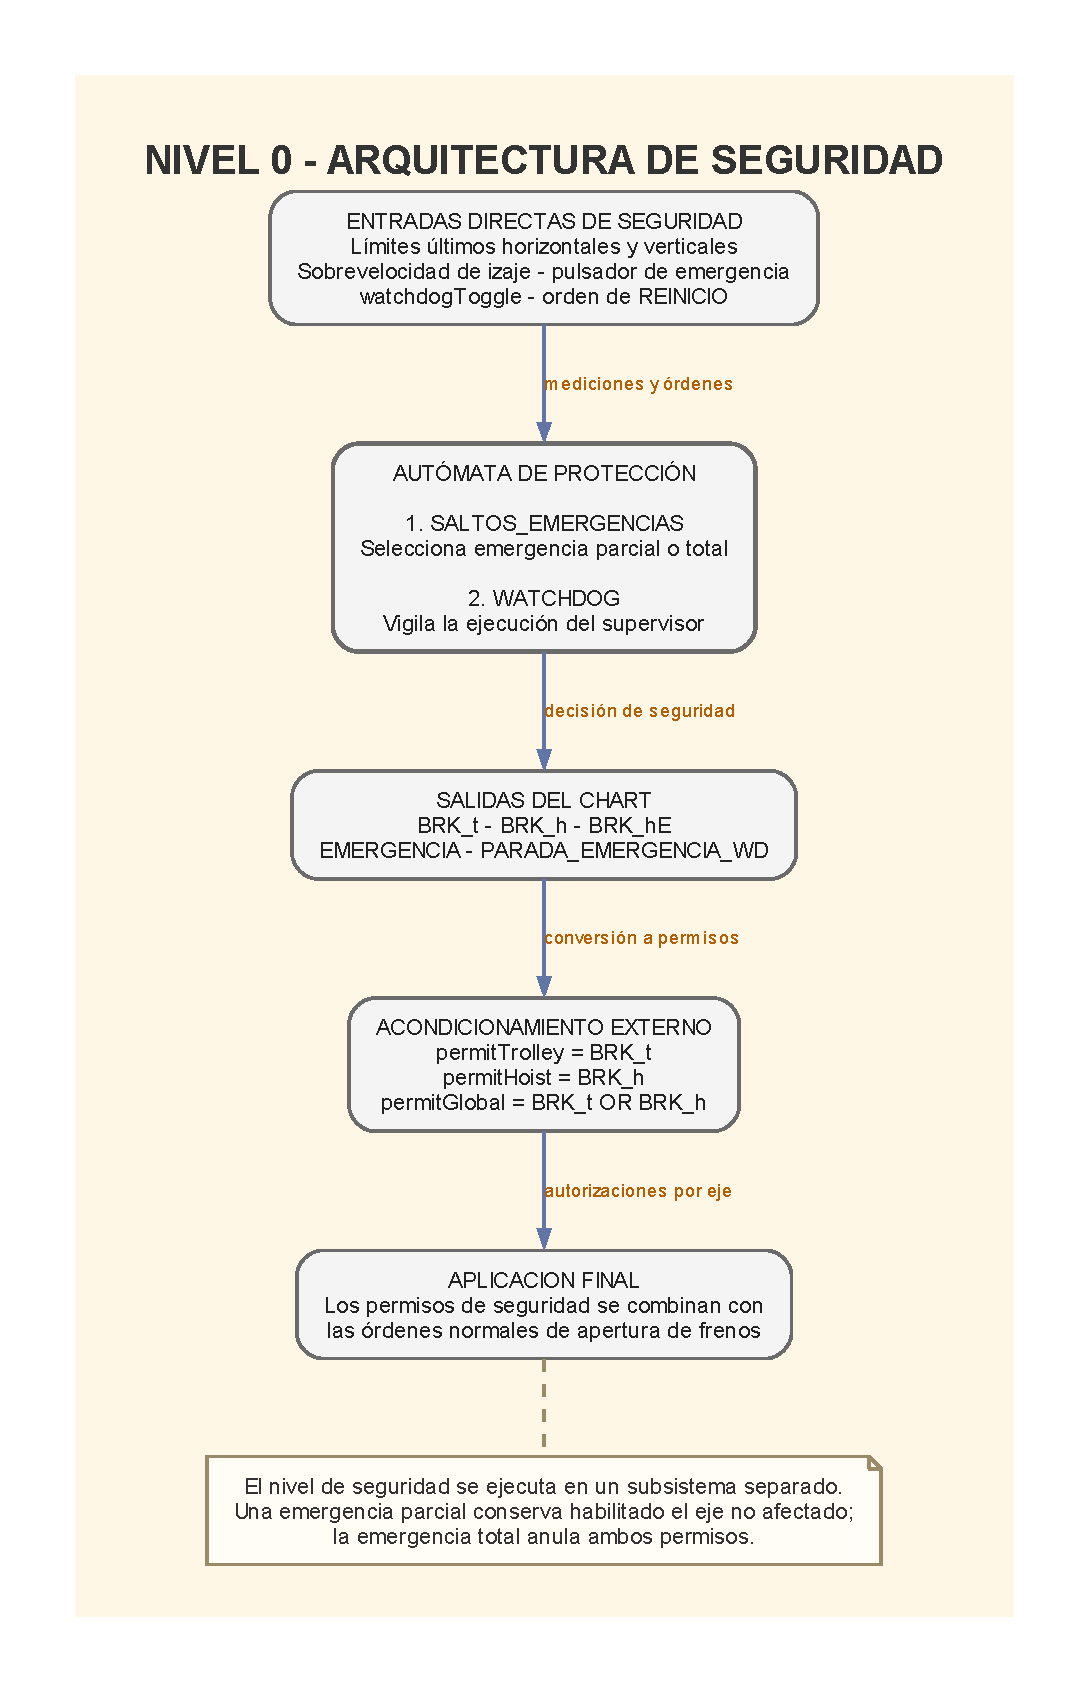
\includegraphics[height=0.60\textheight,keepaspectratio]{imagenes_informe/otro/diagramas_automatas_revision/10_arquitectura_seguridad.pdf}
\caption{Ubicación funcional independiente del nivel de seguridad y flujo de sus señales.}
\label{fig:arquitectura_seguridad_vectorial}
\end{figure}

\Needspace{5\baselineskip}

\subsection{Regiones del autómata de protección}
El Stateflow de seguridad contiene dos regiones paralelas. \texttt{SALTOS\_EMERGENCIAS} selecciona el tipo de emergencia y los frenos afectados. \texttt{WATCHDOG} verifica que el supervisor continúe ejecutándose.

Desde normal, las transiciones de emergencia se evalúan en este orden: emergencia total por pulsador o watchdog (prioridad 1), emergencia de izaje por flancos verticales o sobrevelocidad (prioridad 2) y emergencia del carro por flancos horizontales (prioridad 3). En cada emergencia parcial, el escalamiento a total precede a la recuperación. No se debe interpretar este orden como una evaluación simultánea independiente de todos los límites: si ambos ejes generan flancos en la misma activación desde normal, se toma primero la transición de izaje. El escalamiento posterior requiere el flanco indicado del otro eje o pulsador/watchdog; la matriz siguiente describe las causas reconocidas por esas guardas.

Los estados funcionales se indexan como:
\begin{table}[!htb]
\centering
\caption{Estados del autómata de seguridad.}
\begin{tabular}{C{1.2cm} L{4.5cm} L{7.7cm}}
\toprule
Índice & Estado & Función\\
\midrule
S0 & \texttt{FUNCIONAMIENTO\_NORMAL} & Mantiene verdaderas las tres autorizaciones de apertura.\\
S1 & \texttt{EMERGENCIA\_CARRO} & Inhibe el carro y aplica su freno.\\
S2 & \texttt{EMERGENCIA\_IZAJE} & Inhibe izaje y aplica ambos frenos de izaje.\\
S3 & \texttt{EMERGENCIA\_TOTAL} & Inhibe todos los movimientos y aplica todos los frenos.\\
W0 & \texttt{FUNCIONAMIENTO\_NORMAL} & Reinicia temporización con cada cambio del pulso.\\
W1 & \texttt{FALLO\_WD} & Solicita parada total por pérdida de actividad.\\
\bottomrule
\end{tabular}
\end{table}

\begin{figure}[!htb]
    \centering
    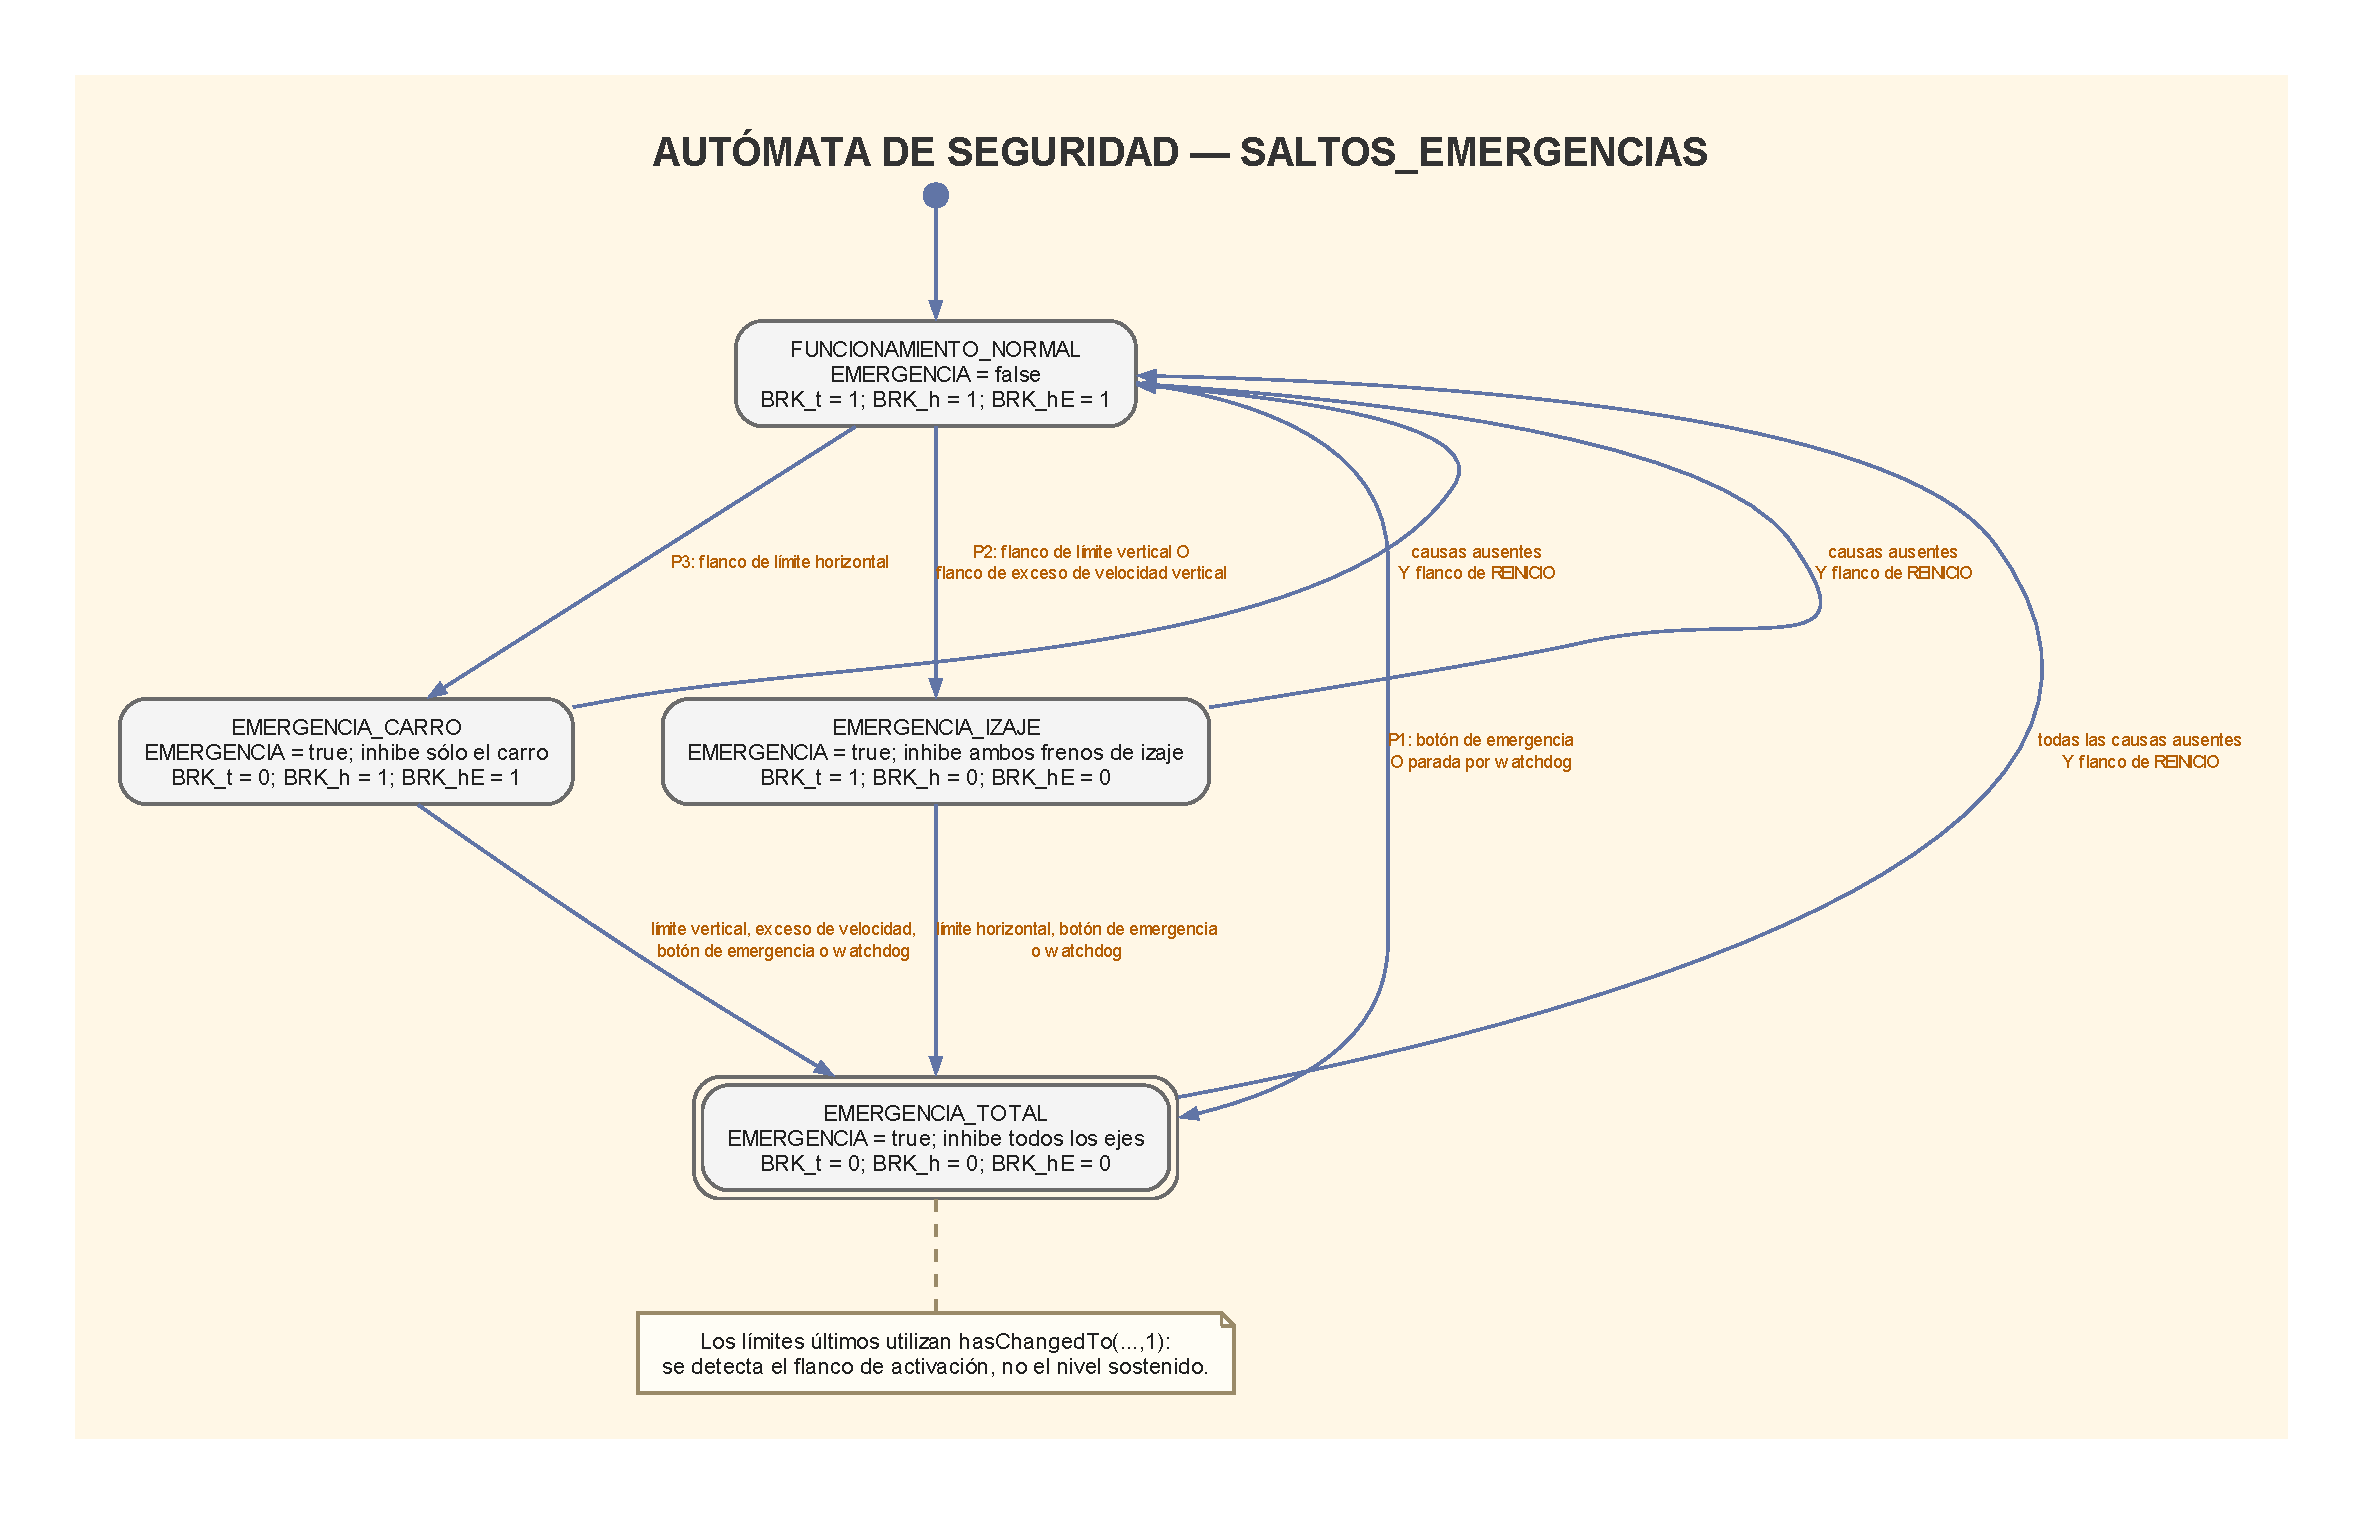
\includegraphics[width=0.98\textwidth,height=0.70\textheight,keepaspectratio]{imagenes_informe/otro/diagramas_automatas_revision/08_seguridad_emergencias.pdf}
    \caption{Máquina de estados de la región \texttt{SALTOS\_EMERGENCIAS}, con prioridades, autorizaciones de freno y recuperación enclavada.}
\label{fig:seguridad_emergencias}
\end{figure}

\Needspace{5\baselineskip}

\subsection{Emergencia del carro}
Desde funcionamiento normal se ingresa a \texttt{EMERGENCIA\_CARRO} mediante \texttt{hasChangedTo(...,1)} sobre cualquiera de los límites últimos horizontales. La condición es sensible al flanco de activación y no sólo al nivel sostenido. En este estado \texttt{EMERGENCIA} pasa a verdadero, \texttt{BRK\_t} pasa a falso y \texttt{BRK\_h} y \texttt{BRK\_hE} permanecen verdaderos. Por lo tanto se aplica el freno del carro y el izaje continúa autorizado.

La recuperación exige que el pulsador de emergencia esté liberado, que ambos límites últimos horizontales estén inactivos y que se detecte un flanco de reinicio. No se permite una recuperación automática por la sola desaparición del límite.

Si durante una emergencia de carro aparece un límite último vertical, exceso de velocidad vertical, pulsador de emergencia o falla de \textit{watchdog}, se escala a \texttt{EMERGENCIA\_TOTAL}.

\Needspace{5\baselineskip}

\subsection{Emergencia de izaje}
La emergencia de izaje se activa por un flanco ascendente del límite último superior, del límite último inferior o de la indicación de exceso de velocidad vertical. En este estado \texttt{BRK\_h} y \texttt{BRK\_hE} pasan a falso, mientras \texttt{BRK\_t} permanece verdadero. Se aplican ambos frenos de izaje y el carro continúa autorizado mientras no aparezca otra condición de emergencia.

Para recuperar se requiere que el pulsador esté liberado, que los límites verticales y la indicación de velocidad máxima estén inactivos y que exista un flanco de reinicio. Si aparece simultáneamente un límite horizontal, una parada de emergencia o una falla de \textit{watchdog}, se pasa a emergencia total.

\Needspace{5\baselineskip}

\subsection{Emergencia total}
La emergencia total se activa directamente por el nivel del pulsador, por \texttt{PARADA\_EMERGENCIA\_WD} o por la aparición de una causa del otro eje mientras existe una emergencia parcial. En este estado \texttt{BRK\_t}, \texttt{BRK\_h} y \texttt{BRK\_hE} son falsos; en consecuencia se inhiben ambos permisos de eje, el permiso global y las tres autorizaciones de apertura de freno.

La recuperación exige que todas las causas hayan desaparecido y que el operador emita una orden de reinicio. La pérdida del permiso global lleva al supervisor a parada normal; al completarla se vuelve a APAGADO y se necesita una nueva orden de marcha.

La combinación de retención en el nivel supervisor y reinicio enclavado en seguridad evita que un sistema que acaba de atravesar una emergencia retome una referencia automática anterior.

\Needspace{5\baselineskip}

\subsection{Watchdog}
El supervisor conmuta una variable booleana en cada ciclo. El nivel de seguridad utiliza la función \texttt{hasChanged} para detectar actividad. Cada cambio realimenta el estado normal del \textit{watchdog} y reinicia su temporización.

En el modelo de referencia \texttt{TiempoMaxWD} vale $5~\mathrm{s}$. Desde el estado normal del watchdog se evalúa primero el vencimiento del tiempo (orden 1) y luego la realimentación por cambio del pulso (orden 2). Si ambas condiciones coinciden, prevalece el fallo.

Si no aparece un cambio antes de \texttt{TiempoMaxWD}, se ingresa a \texttt{FALLO\_WD} y se activa \path{PARADA_EMERGENCIA_WD}. Debido a que \texttt{SALTOS\_EMERGENCIAS} se ejecuta antes que \texttt{WATCHDOG}, la emergencia total reconoce esta salida en la activación siguiente del chart. \texttt{FALLO\_WD} se abandona únicamente ante un flanco ascendente de reinicio.

El mismo orden de regiones afecta la recuperación. Si el sistema se encuentra simultáneamente en \texttt{EMERGENCIA\_TOTAL} y \texttt{FALLO\_WD}, el primer flanco de reinicio puede limpiar el estado del \textit{watchdog} después de que la región de emergencias ya fue evaluada. En ese caso, la salida de emergencia total requiere un nuevo flanco de reinicio con \texttt{PARADA\_EMERGENCIA\_WD} ya en falso.

Este mecanismo detecta tanto la detención del supervisor como una señal congelada. No alcanza con mantener el pulso en uno; debe continuar cambiando.



\begin{figure}[!htb]
    \centering
    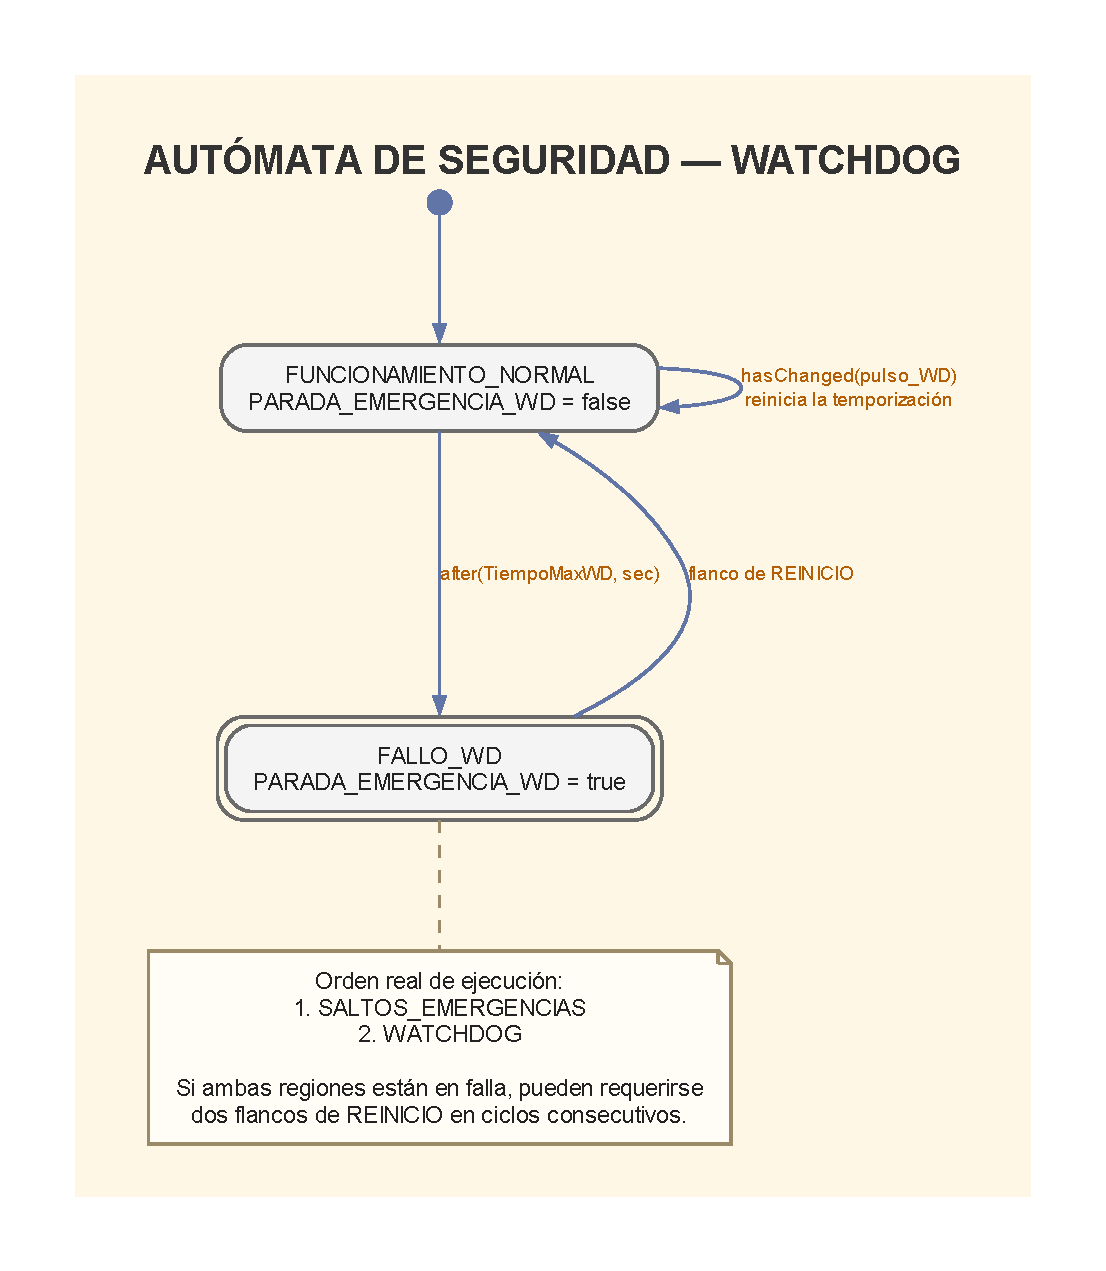
\includegraphics[width=.65\textwidth,height=.43\textheight,keepaspectratio]{imagenes_informe/otro/diagramas_automatas_revision/09_watchdog.pdf}
    \caption{Región \texttt{WATCHDOG}, temporización de actividad y recuperación mediante flanco de reinicio.}
\label{fig:seguridad_watchdog}
\end{figure}

\Needspace{5\baselineskip}

\subsection{Matriz causa--efecto}
\begin{table}[!htb]
\centering
\caption{Respuesta del nivel de seguridad.}
\begin{tabular}{L{4.2cm} C{1.8cm} C{1.8cm} C{1.8cm} C{2.0cm} C{2.0cm}}
\toprule
Causa & Permiso global & Permiso carro & Permiso izaje & Apertura freno carro & Apertura frenos izaje\\
\midrule
Operación normal & Sí & Sí & Sí & Sí & Sí\\
Límite último horizontal & Sí & No & Sí & No & Sí\\
Límite último vertical & Sí & Sí & No & Sí & No\\
Exceso de velocidad vertical & Sí & Sí & No & Sí & No\\
Pulsador de emergencia & No & No & No & No & No\\
Falla de \textit{watchdog} & No & No & No & No & No\\
Emergencia parcial y flanco del otro eje & No & No & No & No & No\\
\bottomrule
\end{tabular}
\end{table}

\Needspace{5\baselineskip}

\subsection{Secuencia de rearme}

El rearme requiere la desaparición de las causas y un flanco de reinicio. Ante una emergencia parcial se restablecen las autorizaciones del eje afectado sin imponer, por esta causa, una nueva secuencia de arranque al eje restante. Después de una emergencia total, el supervisor debe completar la parada y recorrer nuevamente \texttt{APAGADO}, \texttt{ARRANQUE} y \texttt{LISTO} antes de admitir movimiento. Cuando interviene el watchdog, se aplica la secuencia de recuperación descrita en el apartado correspondiente.
\Needspace{5\baselineskip}

\subsection{Aplicación final de las autorizaciones}
Las salidas del autómata de seguridad no reemplazan las órdenes del supervisor. Cada autorización se combina mediante una compuerta lógica AND con la solicitud normal de apertura correspondiente. Las órdenes operativas pueden mantenerse verdaderas durante \texttt{TB\_APLICANDO} o \texttt{HB\_APLICANDO} mientras se completa la detención; no corresponden exclusivamente a los estados \texttt{TB\_ABIERTO} y \texttt{HB\_ABIERTO}. Por tanto, el supervisor puede mantener un freno aplicado aun cuando seguridad lo autorice, pero no puede liberarlo si el nivel de seguridad lo prohíbe.

\begin{figure}[!htb]
\centering
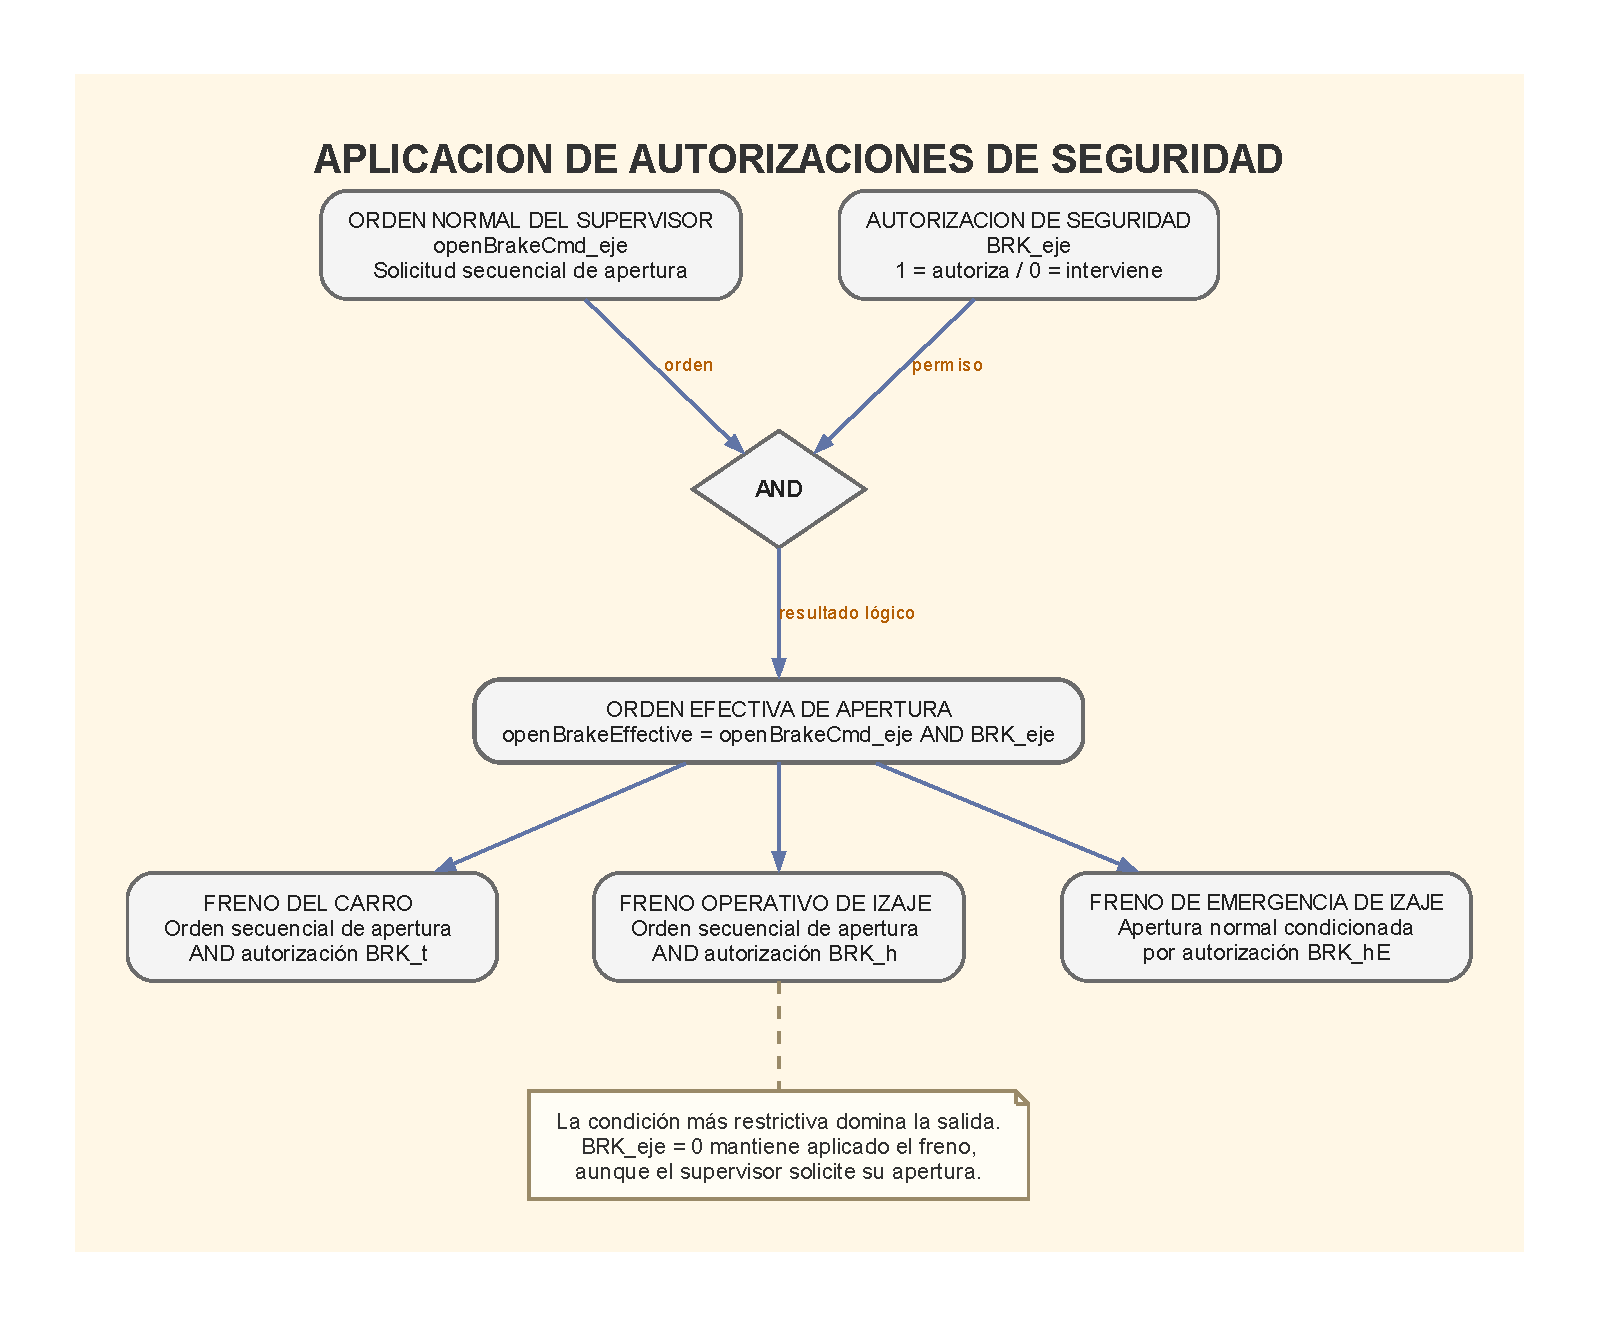
\includegraphics[width=0.98\textwidth,height=0.68\textheight,keepaspectratio]{imagenes_informe/otro/diagramas_automatas_revision/11_compuertas_seguridad.pdf}
\caption{Combinación lógica de las órdenes del supervisor con las autorizaciones del nivel de seguridad.}
\label{fig:compuertas_seguridad_vectorial}
\end{figure}

\Needspace{5\baselineskip}

La validación funcional y el alcance experimental de esta lógica se presentan en el apartado~\ref{sec:validacion_seguridad_stateflow}.

\par
\Needspace{10\baselineskip}
\section{Entorno de visualización e interfaz HMI}
\label{sec:visualizacion_hmi}

\Needspace{5\baselineskip}

\subsection{Representación de la maniobra}

El entorno de visualización ofrece una vista lateral bidimensional de la grúa STS y de su zona de trabajo. Sobre ejes expresados en metros se representan el muelle, el barco y las pilas de contenedores, junto con la estructura de la grúa, el carro, el cable de izaje, el \textit{spreader} y el contenedor suspendido. La posición del carro se muestra sobre la viga; la del \textit{spreader} se obtiene de la posición de la carga. Esta separación permite observar en la escena el desplazamiento relativo asociado al balanceo del cable, además del movimiento horizontal y vertical de la maniobra.

Las alturas de las pilas corresponden al estado físico del entorno simulado y se actualizan cuando se toma o deposita un contenedor. Sobre la misma escena se dibujan dos referencias distintas: la línea horizontal roja indica la cota de cruce alto y la línea escalonada naranja representa la envolvente local de seguridad calculada a partir del perfil de obstáculos, desplazada gráficamente una altura de contenedor. Por lo tanto, la línea naranja permite identificar la cota local de referencia en cada sector, mientras que la roja facilita observar el despeje empleado para el cruce a mayor altura. También se muestra el tiempo de simulación.

La figura~\ref{fig:visualizacion_hmi_perfil} presenta una captura del modelo \path{GruaPerfilSeg_30092026.slx} durante la toma en el muelle. La escena y el panel de operación se muestran en una misma ventana para relacionar el estado físico de la carga con las órdenes y avisos visibles para el operador.

\begin{figure}[!htb]
    \centering
    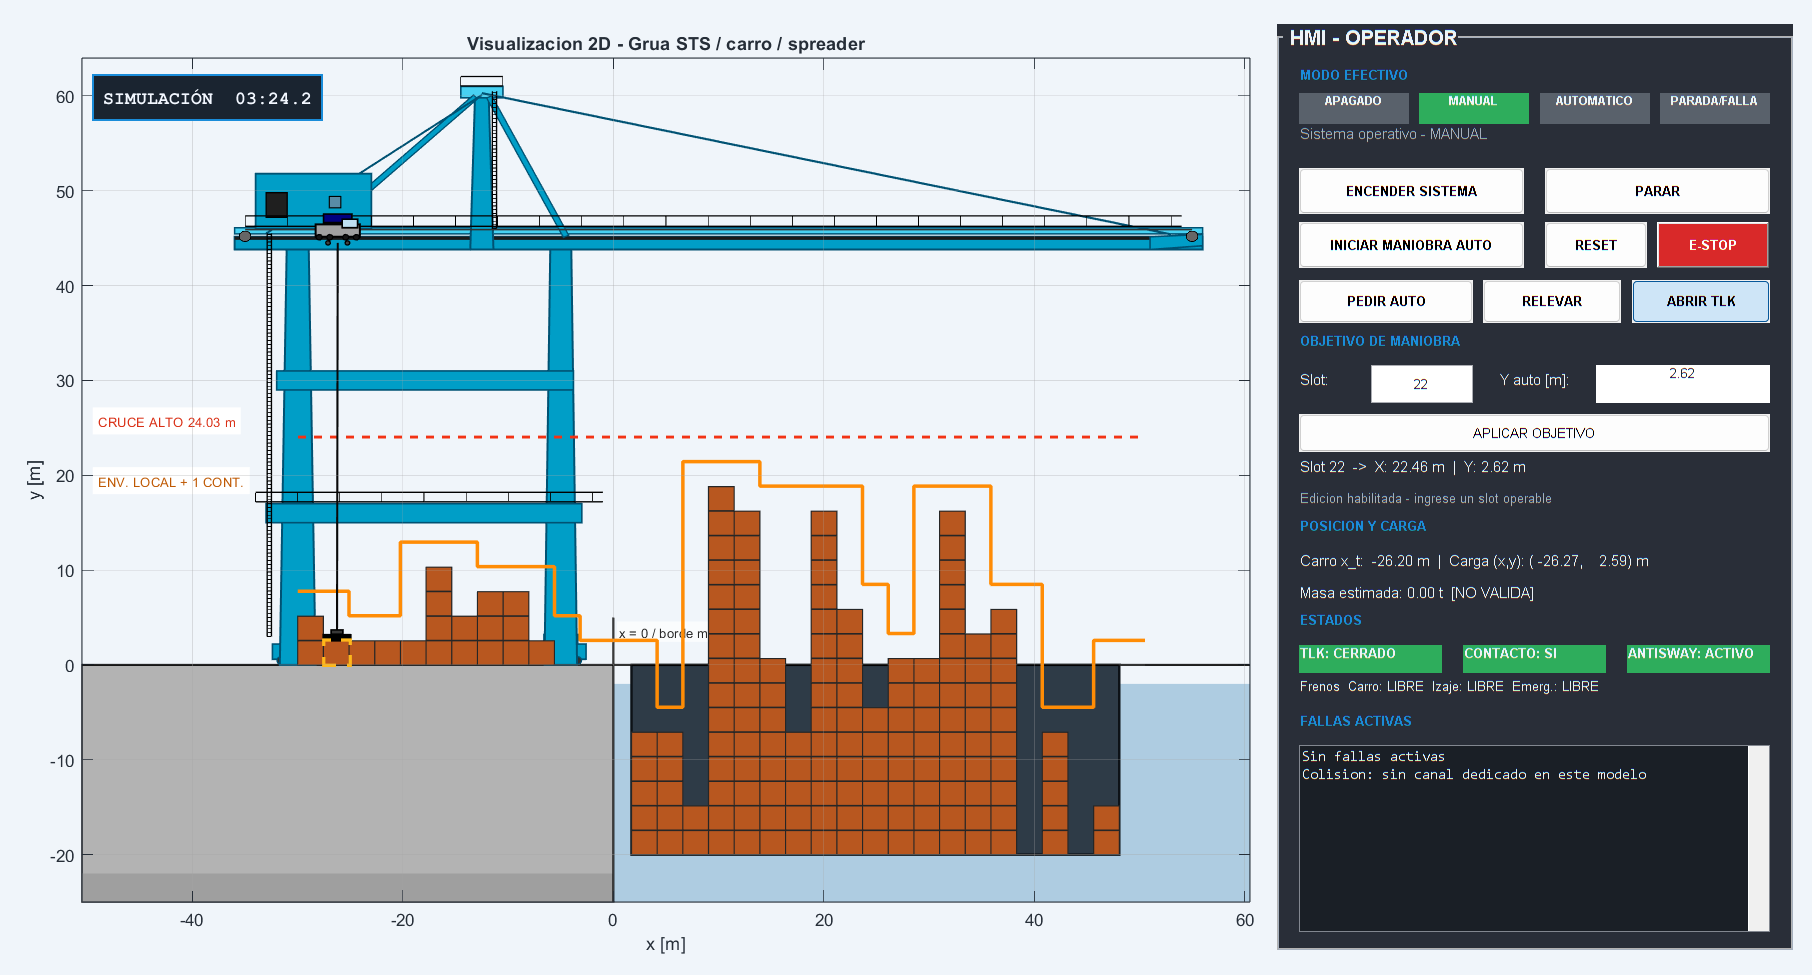
\includegraphics[width=\textwidth]{imagenes_informe/usuario/Visualizacion_HMI_GruaPerfilSeg_30092026.png}
    \caption{Entorno de visualización e interfaz HMI del modelo \texttt{GruaPerfilSeg\_30092026.slx}. La captura muestra la toma en manual, el perfil de contenedores, la envolvente local y la línea de cruce alto.}
    \label{fig:visualizacion_hmi_perfil}
\end{figure}

\Needspace{5\baselineskip}

\subsection{Comandos y avisos de la HMI}

El panel lateral constituye la interfaz hombre--máquina (HMI) del modelo. Desde allí se emiten solicitudes de encendido, parada, parada de emergencia, reinicio, relevamiento, cambio de modo, inicio de la maniobra automática, selección del slot de destino y apertura o cierre de los \textit{twistlocks}. El movimiento manual del carro y del izaje también puede introducirse desde el teclado. La HMI entrega estas solicitudes como señales a la lógica de mando y supervisión; el modo mostrado como efectivo corresponde al estado informado por el autómata, no simplemente al botón accionado.

El mismo panel informa la posición del carro y de la carga, el objetivo seleccionado, la estimación de masa y su validez, el contacto con el contenedor, el estado de los \textit{twistlocks} y del antisway, la condición de los frenos y los avisos de falla. Esto permite seguir la secuencia de toma, traslado y entrega y reconocer cuándo una orden solicitada aún no se ha convertido en un cambio de estado efectivo. La HMI es, por tanto, tanto un medio de operación durante la simulación como un instrumento para interpretar sus resultados.

\Needspace{5\baselineskip}

\subsection{Construcción mediante una S-Function de nivel 2}

La visualización se implementó como una \textit{S-Function} MATLAB de nivel 2, contenida en \path{visualizacion_modelo_final_hmi_corregido.m} e integrada al diagrama de Simulink. La función \texttt{setup} declara 42 puertos de entrada y 15 de salida, sus dimensiones y tipos, y el período de muestreo \texttt{Pvis.Ts\_viz} (con un valor de reserva de 0,05~s). Entre las entradas se encuentran las posiciones necesarias para animar la grúa, el perfil físico de contenedores, la envolvente local de 33 slots, la cota de cruce alto y las señales de modo, carga, sensores, frenos y fallas. Las salidas publican las órdenes formuladas en la HMI.

La programación se organiza alrededor de los métodos \texttt{Start}, \texttt{Outputs}, \texttt{Update} y \texttt{Terminate} registrados por la S-Function. Al comenzar la simulación, \texttt{Start} crea la figura, dibuja la geometría fija y las pilas iniciales, prepara los objetos gráficos móviles y construye el panel de controles. Los identificadores de estos objetos se conservan para reutilizarlos en cada paso, sin reconstruir toda la ventana. Los botones y teclas modifican el estado de la interfaz mediante funciones de retorno de llamada; \texttt{Outputs} transforma ese estado en las señales de solicitud que recibe el modelo. Las órdenes momentáneas se publican como pulsos y se limpian posteriormente en \texttt{Update}.

En cada actualización, \texttt{Update} modifica las propiedades gráficas de los objetos existentes con las señales actuales: desplaza el carro, el cable, el \textit{spreader} y la carga; redibuja la altura de cada pila; sitúa las líneas de cruce y envolvente; y renueva los indicadores y avisos de la HMI. La animación se limita mediante \texttt{drawnow limitrate} para evitar redibujos innecesarios. Esta organización mantiene vinculados los elementos visuales, las órdenes del operador y la evolución temporal de la simulación en un único bloque, mientras el control y las decisiones de seguridad permanecen en sus subsistemas correspondientes.

\par
\Needspace{10\baselineskip}
\section{Integración y evaluación del desempeño en Simulink (MIL)}
\label{sec:integracion_p1}
La etapa \textit{model in the loop} (MIL) evalúa la planta, los reguladores y los autómatas dentro de MATLAB/Simulink. Este apartado desarrolla la validación regulatoria con referencias aisladas y las iteraciones de diseño realizadas durante la integración. Las pruebas del autómata de seguridad, el ciclo completo MIL y los ensayos de medio ciclo CODESYS se reúnen en la sección~\ref{sec:pruebas_sistema}, después de presentar las implementaciones. Cada ensayo conserva su configuración y su alcance.

\Needspace{5\baselineskip}

\subsection{Validación regulatoria con referencias aisladas}
\label{subsec:validacion_regulatoria_MIL}
	\Needspace{5\baselineskip}
	\subsubsection{Condiciones de los ensayos}
	Se realizó una batería de pruebas y ensayos para ajustar el comportamiento de los lazos de control al desempeño deseado. Las referencias de movimiento empleadas fueron análogas a las producidas por el generador de trayectorias, polinomiales y respetaron los límites del generador original. Las corridas aisladas caracterizan los reguladores; la coordinación, el despeje y las transferencias entre modos requieren evaluaciones propias del sistema integrado.
	
	\Needspace{5\baselineskip}
	
	\subsubsection{Izaje cargado y vacío}
	Se compararon dos referencias suaves, cada una con un contenedor de 50~t y sin él. La primera sube de 25 a 27~m en 10~s, sostiene 5~s y baja en 10~s. La segunda baja de 25 a 17~m con velocidad de referencia máxima de 1,2~m/s y aceleración máxima de 0,729~m/s$^2$. Las figuras~\ref{fig:izaje} y \ref{fig:izaje-bajada8} muestran referencias, medidas de altura y velocidad, y torque físico. La tabla~\ref{tab:izaje} resume las métricas durante el movimiento.
	\begin{table}[H]
		\centering\small
		\caption{Seguimiento vertical de los dos perfiles de izaje.}
		\begin{tabular}{llrrrr}
			\toprule
			Perfil & Carga & RMS altura (m) & Error máx. (m) & Torque máx. (kN\,m) & Cuerda floja (s)\\
			\midrule
			Subida y bajada & 50~t & 0,1004 & 0,1235 & 11,65 & 0\\
			Subida y bajada & Vacío & 0,0258 & 0,0460 & 3,18 & 0\\
			Bajada 8~m & 50~t & 0,1487 & 0,1743 & 12,84 & 0\\
			Bajada 8~m & Vacío & 0,0689 & 0,0900 & 3,81 & 0\\
			\bottomrule
		\end{tabular}
		\label{tab:izaje}
	\end{table}
	No se registró saturación de torque durante el movimiento en ninguno de los cuatro casos. Los errores verticales incluyen la elasticidad del cable y el movimiento de la carga: no deben confundirse con los polos del modelo de $l_h$.
	
	En el panel inferior de cada figura se superponen dos corridas del \emph{torque físico del motor de izaje}: la curva azul corresponde al spreader sin contenedor y la naranja al spreader con un contenedor de 50~t. No representan, respectivamente, el torque comandado y el físico. La carga mayor requiere más torque incluso durante el sostén a altura constante, con los frenos liberados. El pico cercano a $t=0$ pertenece al transitorio de inicialización, anterior al comienzo del perfil en $t=5$~s; los máximos de la tabla se calcularon únicamente durante el movimiento. El torque comandado se conservó por separado en las señales del ensayo.
	\begin{figure}[H]
		\centering
		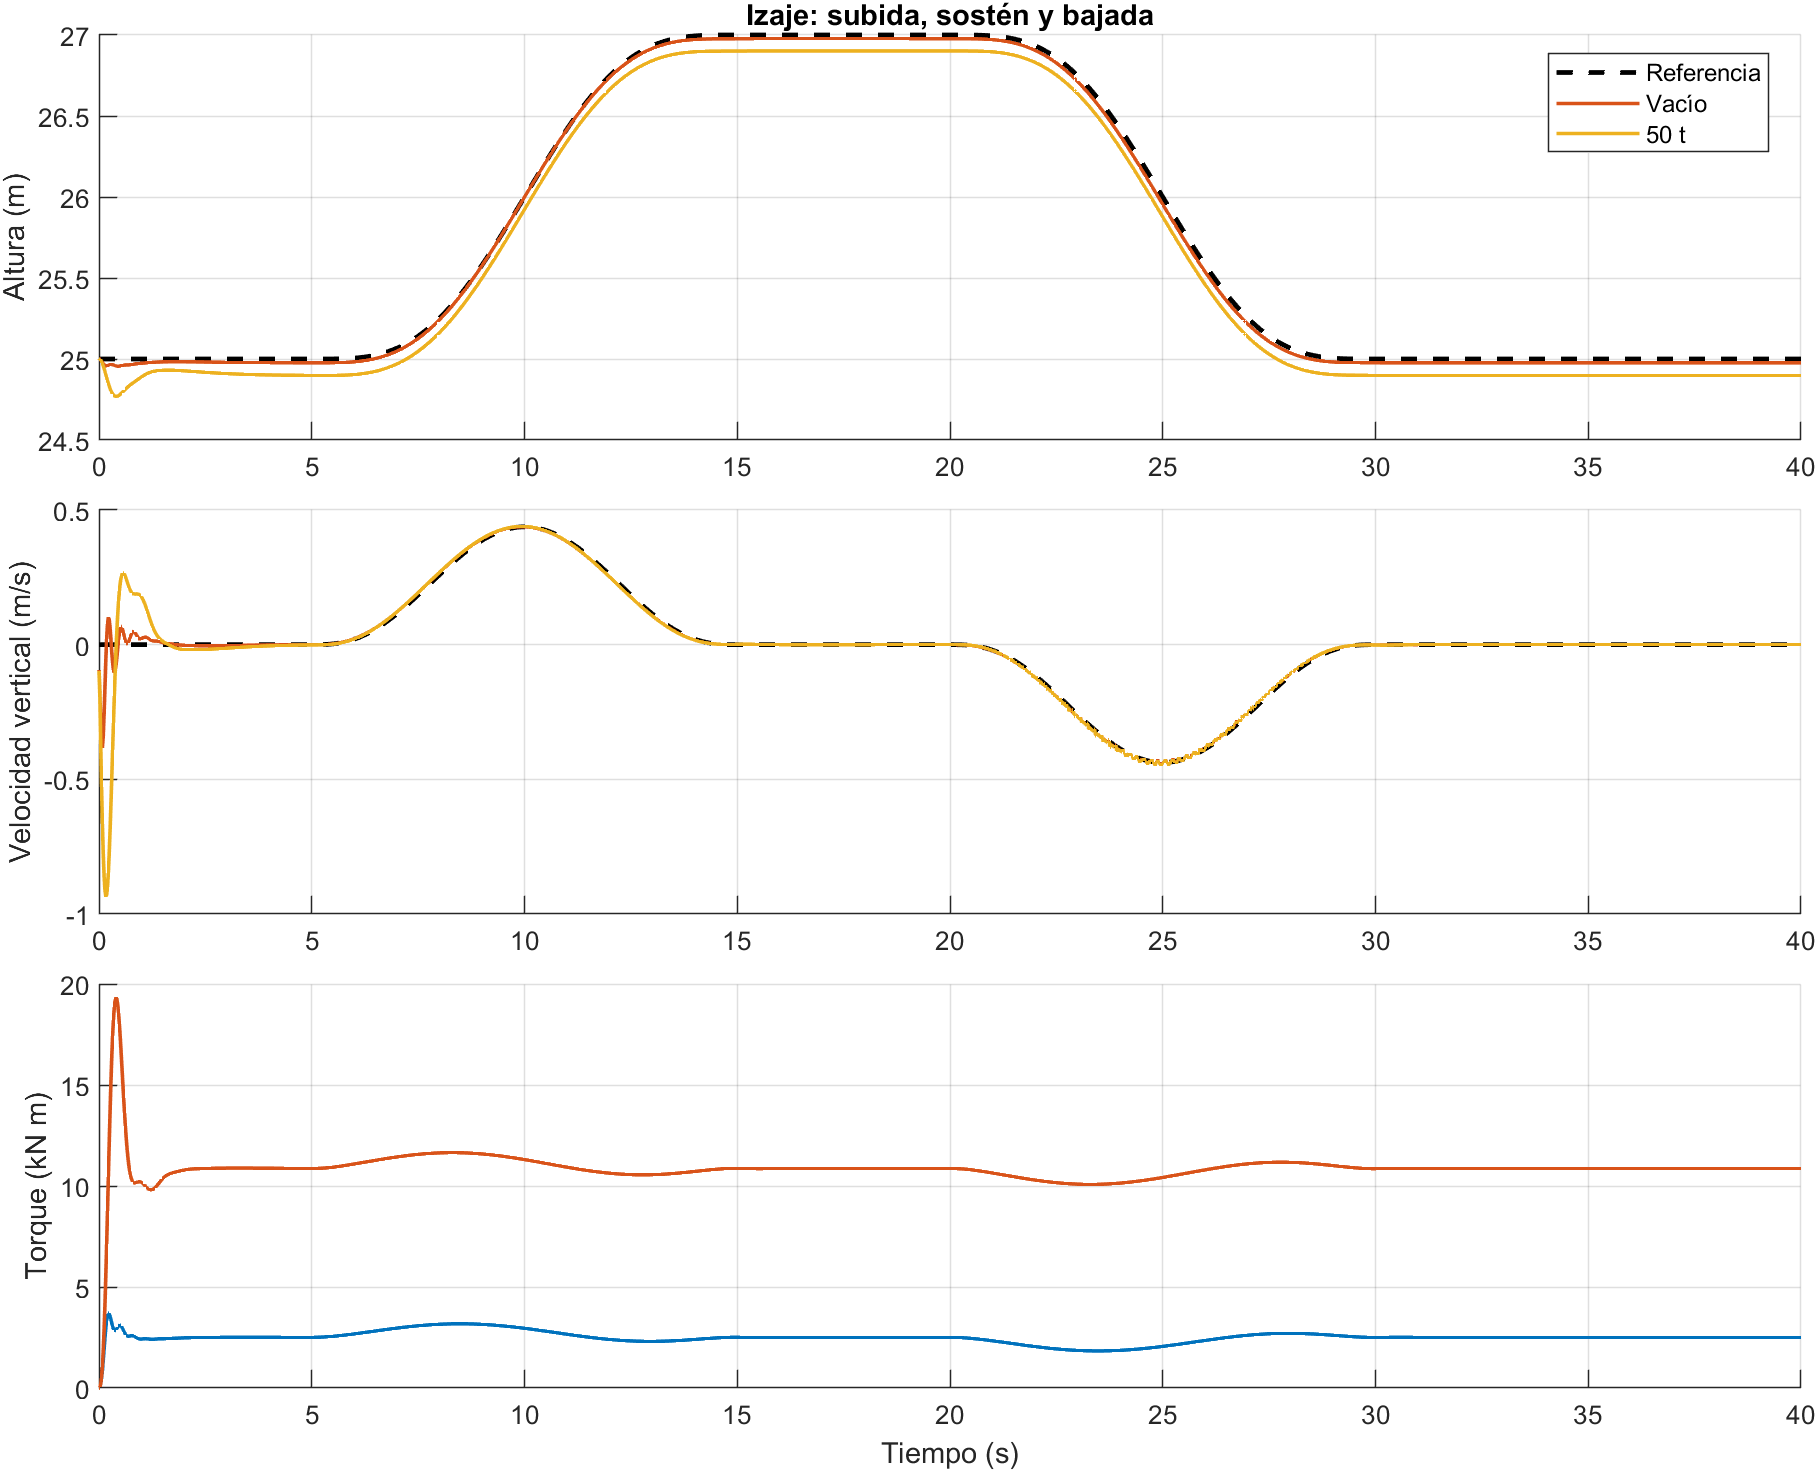
\includegraphics[width=0.82\linewidth]{imagenes_informe/usuario/ensayos_regulatorios_aislados/izaje_original.png}
		\caption{Perfil de subida, sostén y bajada: altura y velocidad de referencia y medida, y torque.}
		\label{fig:izaje}
	\end{figure}
	
	\begin{figure}[H]
		\centering
		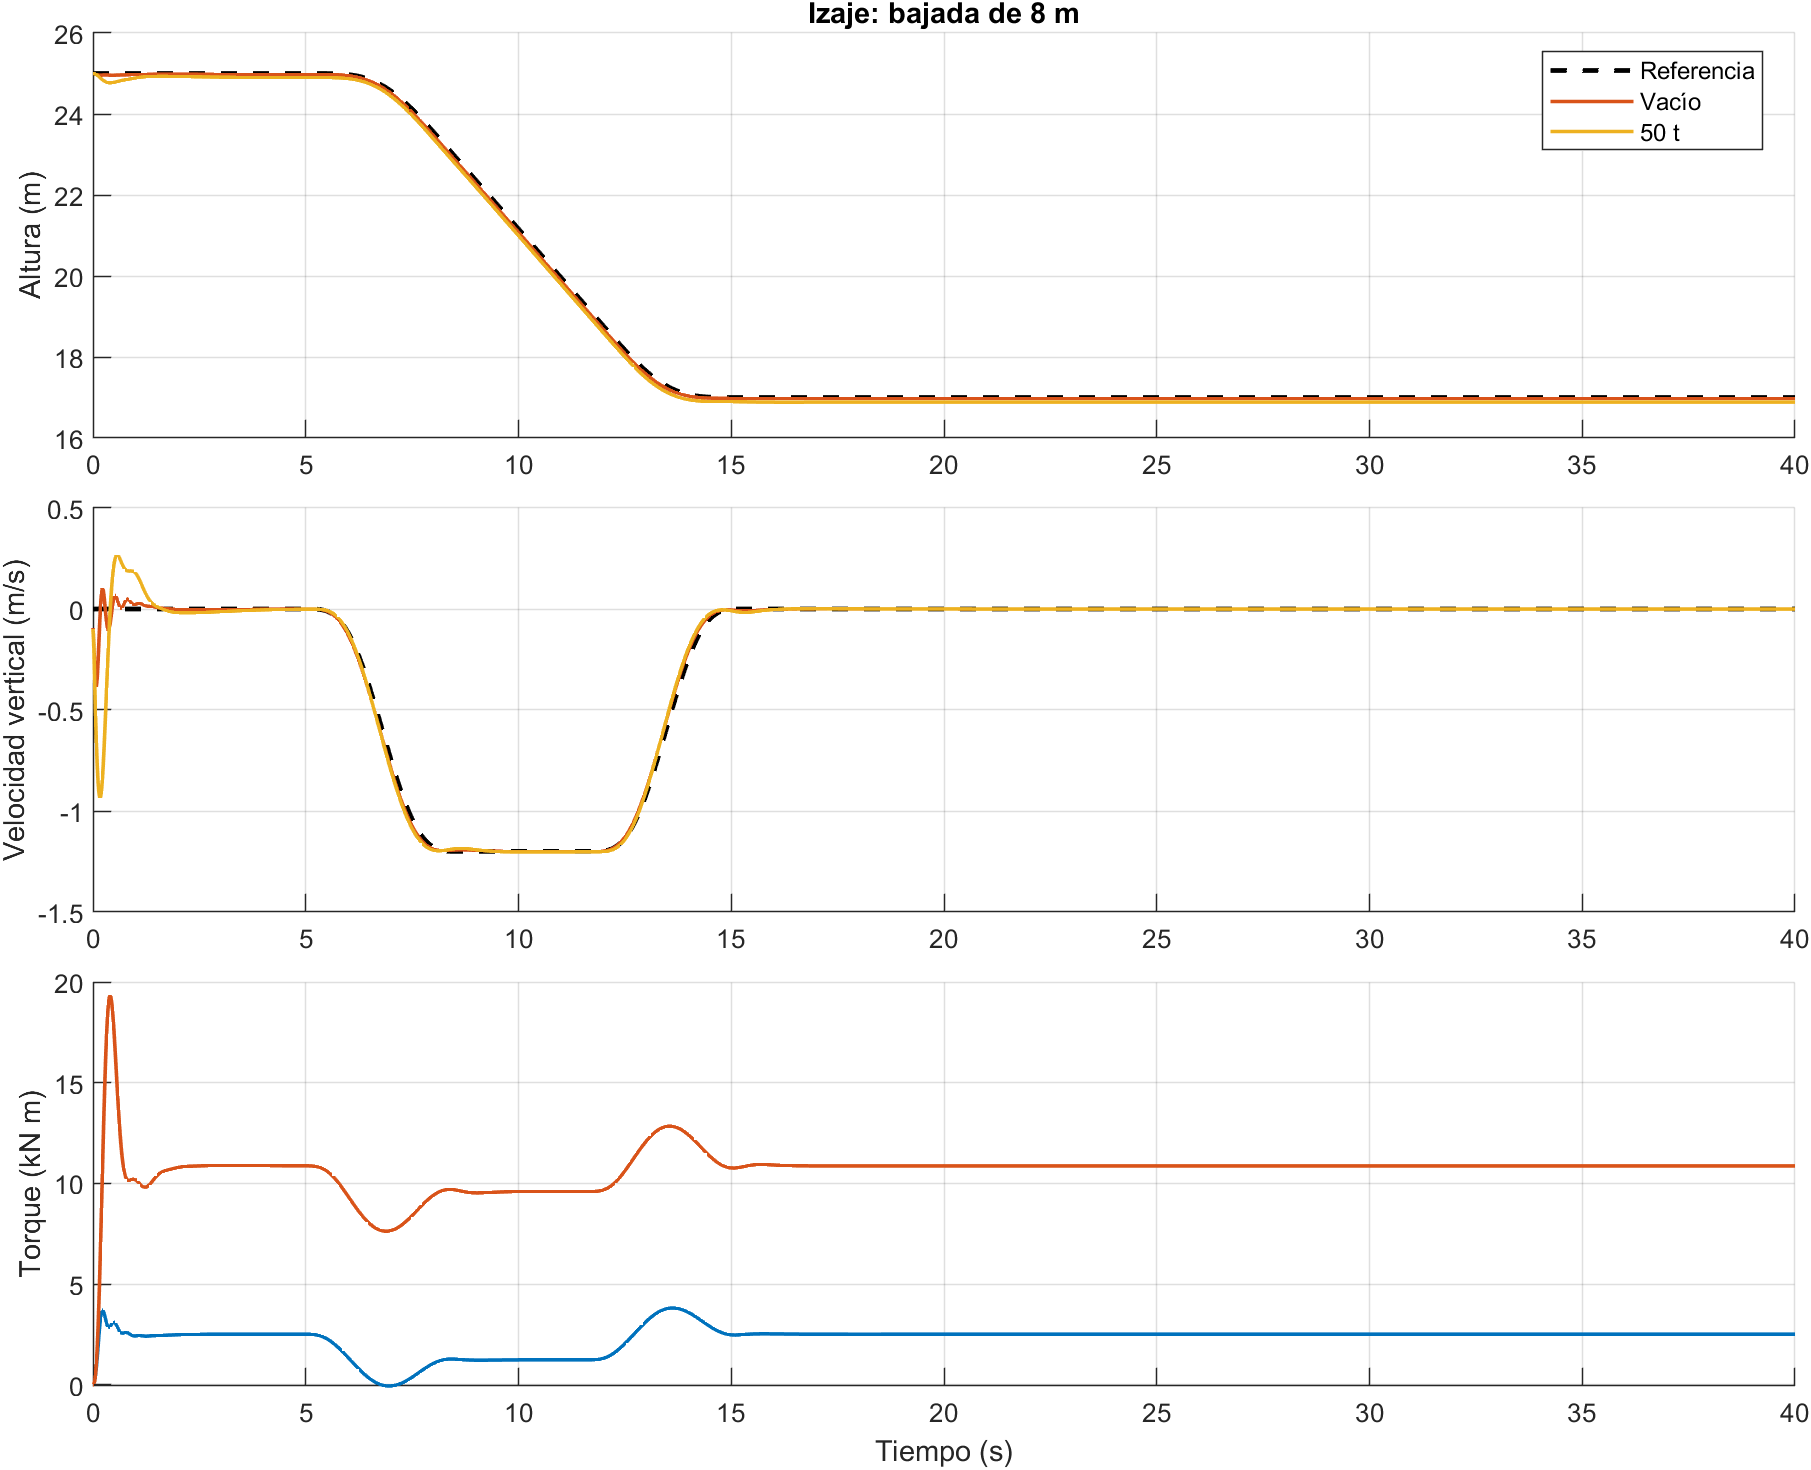
\includegraphics[width=0.82\linewidth]{imagenes_informe/usuario/ensayos_regulatorios_aislados/izaje_bajada8.png}
		\caption{Bajada de 8~m: altura y velocidad de referencia y medida, y torque.}
		\label{fig:izaje-bajada8}
	\end{figure}
	
	\Needspace{5\baselineskip}
	
	\subsubsection{Decaimiento con referencia angular fija}
	Se ensayaron $2^\circ$, $5^\circ$ y $7^\circ$ de perturbación inicial, con 50~t y longitudes de 20 y 25~m. En cada condición se mantuvieron fijas las referencias y se compararon $\zeta_{sw}=0$ (acción desactivada), $0,8$ y $1,75$, correspondientes a $2\zeta_{sw}=0$, $1,6$ y $3,5$. Los frenos estuvieron liberados, la rampa anti-sway se puenteó y la aceleración total aplicada se limitó a $\pm0,8~\mathrm{m/s^2}$. La tabla~\ref{tab:decaimiento-nuevo} recoge el caso más exigente; las curvas de la figura~\ref{fig:decaimiento-nuevo} muestran las dos longitudes.
	
	\begin{table}[H]
		\centering\small
		\caption{Decaimiento desde $7^\circ$ con 50~t, sin rampa anti-sway.}
		\begin{tabular}{rrrrrr}
			\toprule
			Cable (m) & $\zeta_{sw}$ diseño & Primer pico ($^\circ$) & $\zeta_{1/2}$ observado & Establecimiento (s) & Torque máx. (Nm)\\
			\midrule
			20 & 0 & 6,33 & 0,032 & No en 45~s & 1573\\
			20 & 0,8 & 5,06 & 0,103 & 13,14 & 680\\
			20 & 1,75 & 6,24 & 0,036 & 23,68 & 969\\
			25 & 0 & 6,46 & 0,026 & No en 45~s & 1624\\
			25 & 0,8 & 5,08 & 0,102 & 18,22 & 728\\
			25 & 1,75 & 6,01 & 0,049 & 23,58 & 1057\\
			\bottomrule
		\end{tabular}
		\label{tab:decaimiento-nuevo}
	\end{table}
	
	El establecimiento se define por permanencia dentro de $\pm0,05^\circ$. La columna $\zeta_{1/2}$ es una equivalencia calculada desde el ángulo inicial y el primer pico opuesto: si $\delta=\ln(|\theta_0|/|\theta_1|)$, entonces $\zeta_{1/2}=\delta/\sqrt{\pi^2+\delta^2}$. No es el amortiguamiento modal de la planta completa. El límite de aceleración actuó en las corridas con control; a $7^\circ$ y $\zeta_{sw}=1,75$ permaneció activo en el 37--43\% de las muestras. También actuó el límite de amplitud de la acción anti-sway de $3,2$~m/s durante el 12--15\% de esas corridas. Esta asignación dejó un primer pico mayor que $\zeta_{sw}=0,8$ en las seis condiciones de ángulo y longitud. El decremento logarítmico de la envolvente completa se informa solo cuando hay suficientes máximos comparables.
	
	\begin{figure}[H]
		\centering
		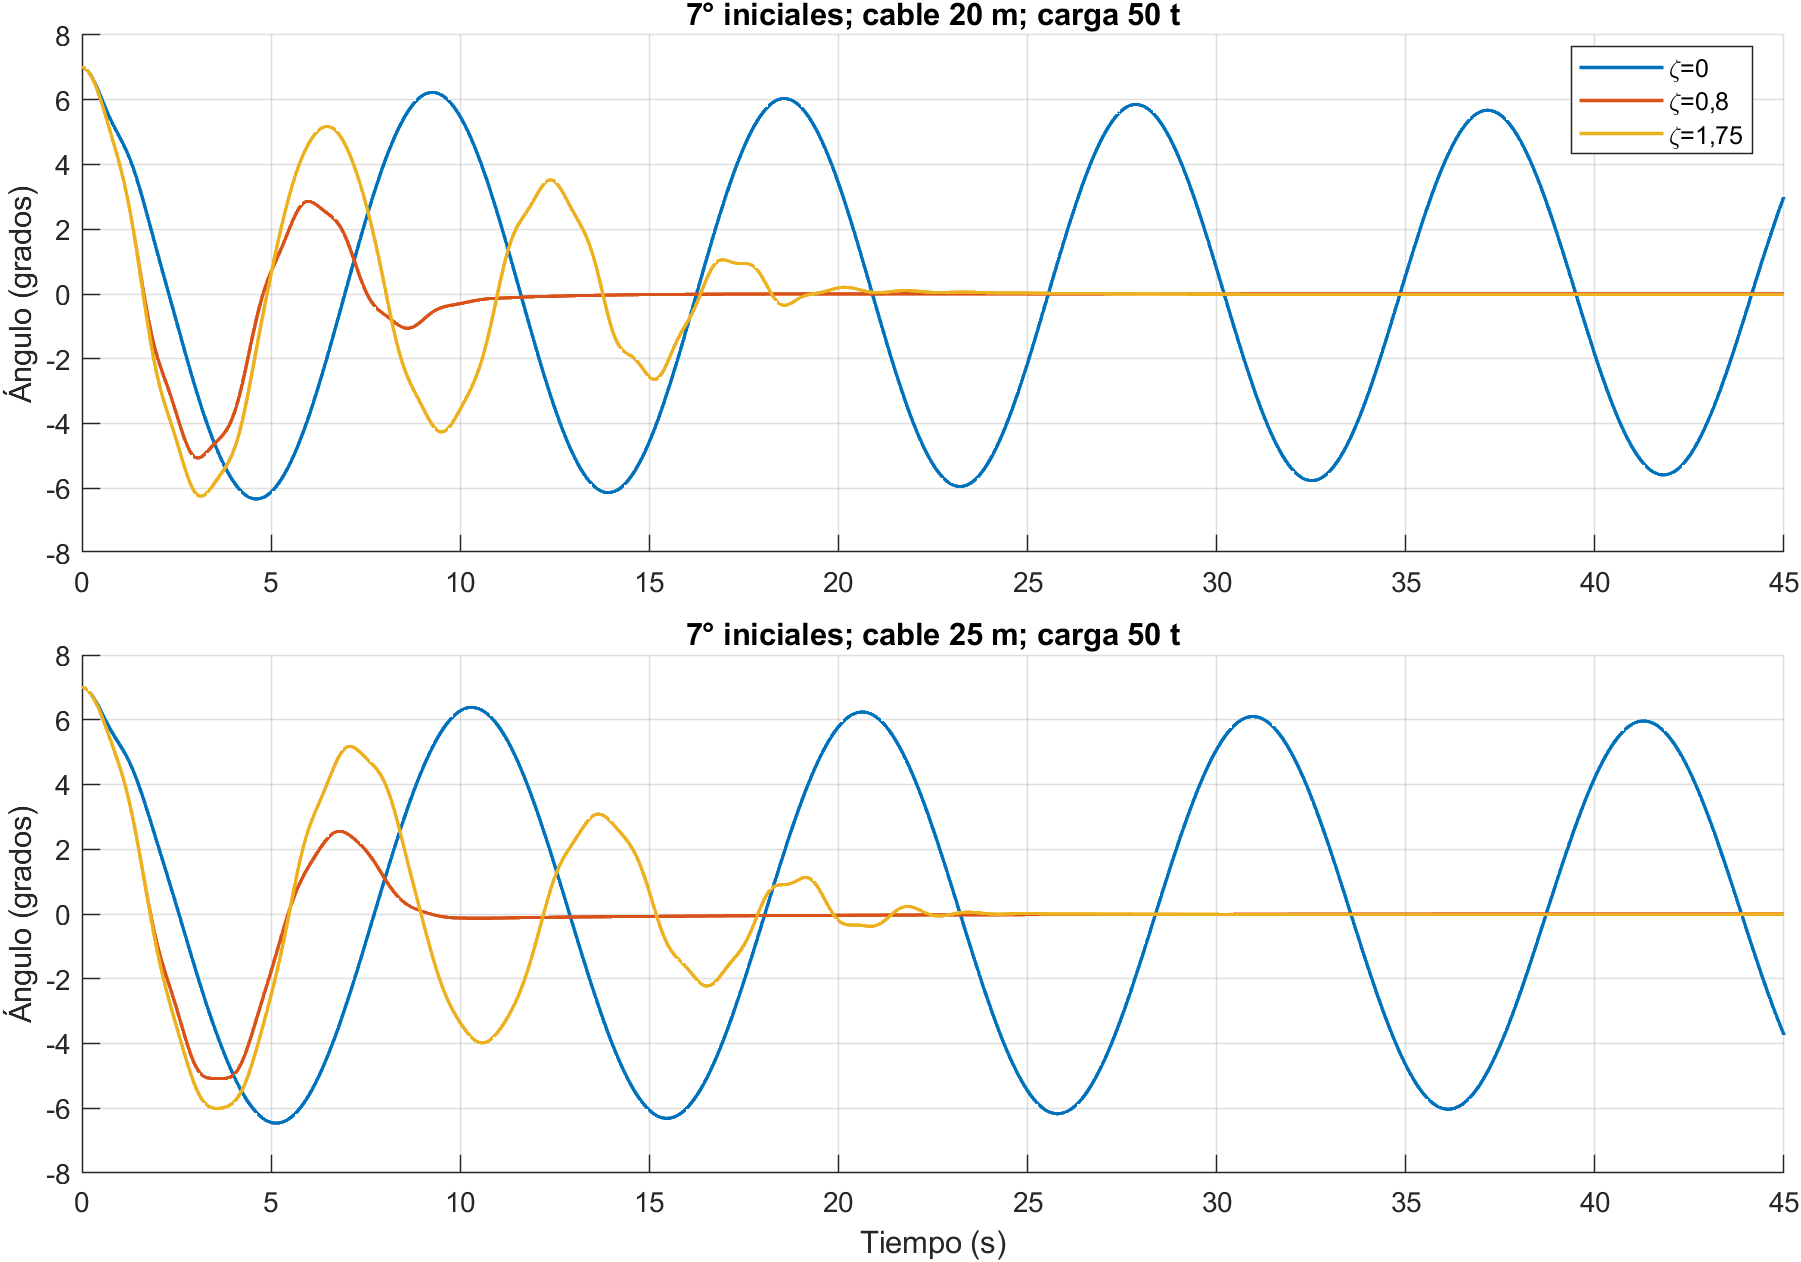
\includegraphics[width=0.82\linewidth]{imagenes_informe/usuario/ensayos_regulatorios_aislados/decaimiento_7grados.png}
		\caption{Decaimiento desde $7^\circ$ a dos longitudes; $\zeta_{sw}$ indica la asignación teórica, no el amortiguamiento medido.}
		\label{fig:decaimiento-nuevo}
	\end{figure}
	
	\Needspace{5\baselineskip}
	
	\subsubsection{Traslado de 13 m con cable de 20 m}
	Se fijaron 20~m de cable, 50~t, $\theta_l(0)=0$, traslado de 13~m en 24~s y $K_{pv}=2,4$, $K_{iv}=0,2$, $K_x=0,05$. Se puenteó físicamente la rampa anti-sway y se compararon, con la misma referencia y el mismo límite total de aceleración $\pm0,8~\mathrm{m/s^2}$, $\zeta_{sw}=0$, $0,8$ y $1,75$. La figura~\ref{fig:traslado-13} incluye posición, velocidad, ángulo y torque. En movimiento, la métrica angular es $\theta_l-\theta_{ref}(t)$; la referencia angular varía durante la aceleración y el frenado.
	\begin{table}[H]
		\centering\small
		\caption{Comparación del traslado de 13~m, 20~m de cable y 50~t.}
		\begin{tabular}{rrrrr}
			\toprule
			$\zeta_{sw}$ & RMS carro (m) & RMS $\theta_l-\theta_{ref}$ ($^\circ$) & Máx. error angular ($^\circ$) & Torque máx. (Nm)\\
			\midrule
			0 & 0,0424 & 1,4536 & 3,27 & 804,3\\
			0,8 & 0,1320 & 0,2100 & 0,405 & 562,8\\
			1,75 & 0,1668 & 0,1051 & 0,200 & 524,2\\
			\bottomrule
		\end{tabular}
		\label{tab:traslado-13}
	\end{table}
	La acción anti-sway redujo el error angular respecto del caso apagado. Al pasar de $\zeta_{sw}=0,8$ a $1,75$, el RMS angular se redujo aproximadamente a la mitad, mientras el RMS de posición del carro aumentó 0,035~m. El torque RMS durante el movimiento fue 462, 321 y 310~Nm, respectivamente; no hubo saturación de torque ni actuó el límite de aceleración. El resultado favorece $\zeta_{sw}=1,75$ si se prioriza el error angular de \emph{este} traslado, pero no la recuperación desde una perturbación inicial grande.
	\begin{figure}[H]
		\centering
		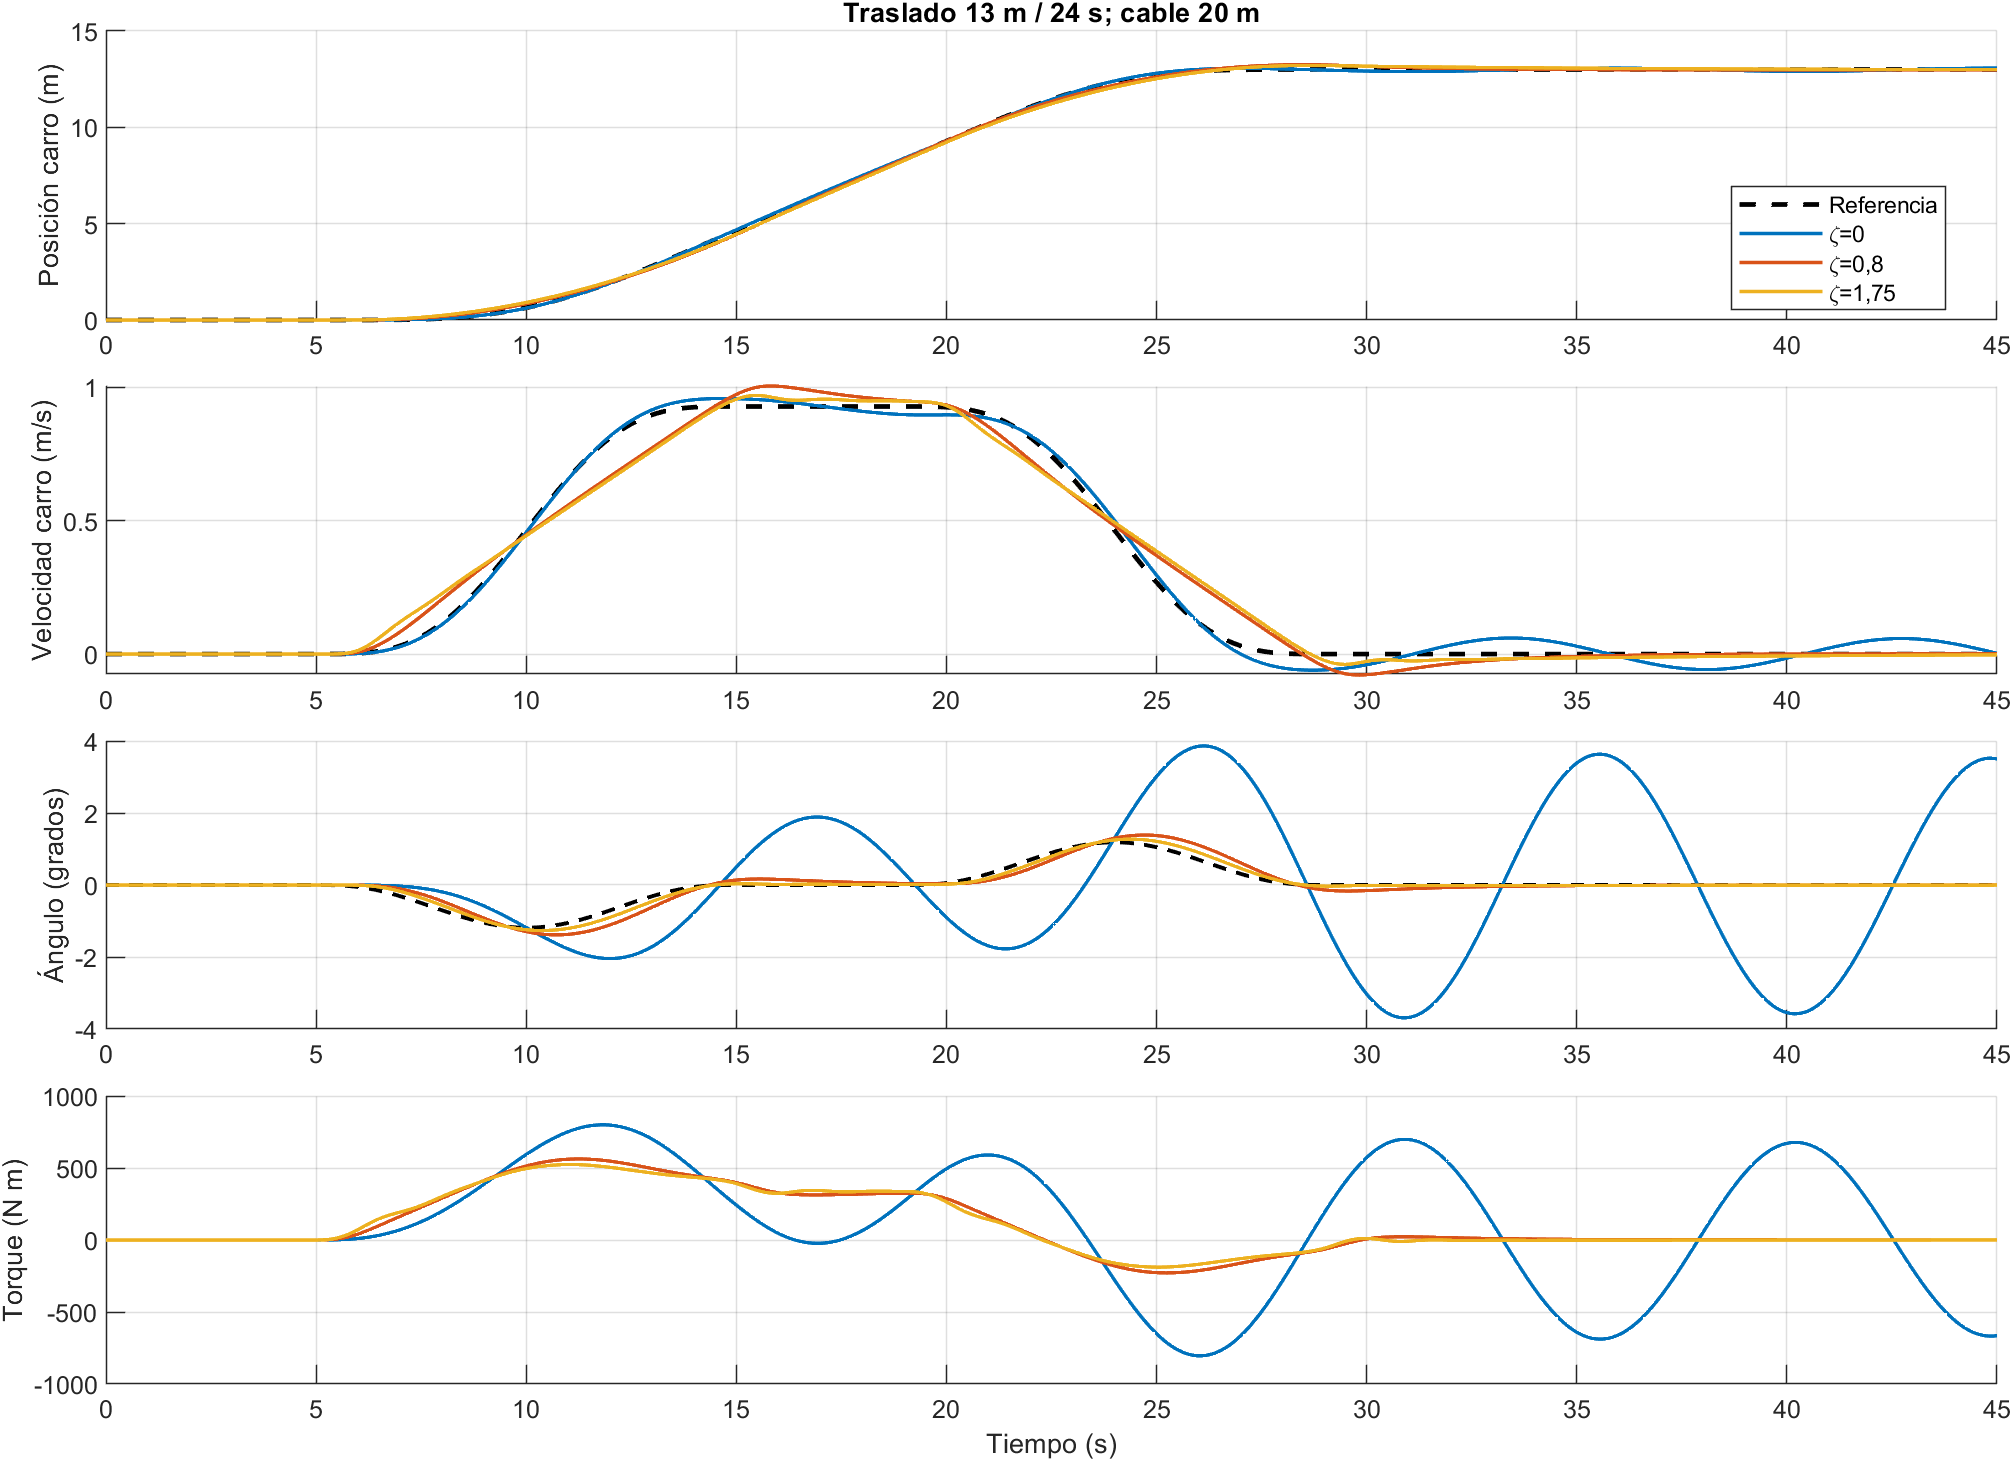
\includegraphics[width=0.82\linewidth]{imagenes_informe/usuario/ensayos_regulatorios_aislados/carro_13m_normal.png}
		\caption{Traslado de 13~m en 24~s: seguimiento de posición y velocidad del carro, ángulo y torque para tres asignaciones de $\zeta_{sw}$.}
		\label{fig:traslado-13}
	\end{figure}
	
	\Needspace{5\baselineskip}
	
	\subsubsection{Traslado más rápido de 13 m con cable de 10 m}
	Se mantuvieron la distancia de 13~m y los 50~t, pero la longitud del cable fue 10~m. La referencia alcanzó 2,85~m/s y una aceleración máxima de 0,792~m/s$^2$. Su aceleración tiene transiciones polinomiales de quinto orden y el movimiento dura aproximadamente 8,66~s. Se repitieron $\zeta_{sw}=0$, $0,8$ y $1,75$, sin rampa y con el mismo límite total de aceleración. La tabla~\ref{tab:traslado-rapido} y la figura~\ref{fig:traslado-rapido} muestran el compromiso entre seguimiento y balanceo.
	
	\begin{table}[H]
		\centering\small
		\caption{Traslado rápido de 13~m, 10~m de cable y 50~t.}
		\begin{tabular}{rrrrr}
			\toprule
			$\zeta_{sw}$ & RMS carro (m) & RMS $\theta_l-\theta_{ref}$ ($^\circ$) & Error máx. carro (m) & Torque máx. (Nm)\\
			\midrule
			0 & 0,274 & 6,647 & 0,53 & 3472\\
			0,8 & 0,945 & 2,314 & 1,86 & 2655\\
			1,75 & 1,627 & 2,037 & 2,78 & 2366\\
			\bottomrule
		\end{tabular}
		\label{tab:traslado-rapido}
	\end{table}
	
	El control redujo el error angular, pero con una pérdida considerable de seguimiento del carro. La aceleración aplicada alcanzó el límite de $0,8~\mathrm{m/s^2}$ en las tres configuraciones; estuvo allí durante el 64\%, 56\% y 77\% de las muestras de movimiento para $\zeta_{sw}=0$, $0,8$ y $1,75$, respectivamente. Las aceleraciones solicitadas por el controlador fueron mayores. La velocidad real osciló y se separó de la referencia, sobre todo con $\zeta_{sw}=1,75$. Por ello ninguna de las dos sintonías controladas demuestra un buen compromiso operativo para este perfil rápido, aunque el torque físico permaneció por debajo de 4~kN\,m.
	
	\begin{figure}[H]
		\centering
		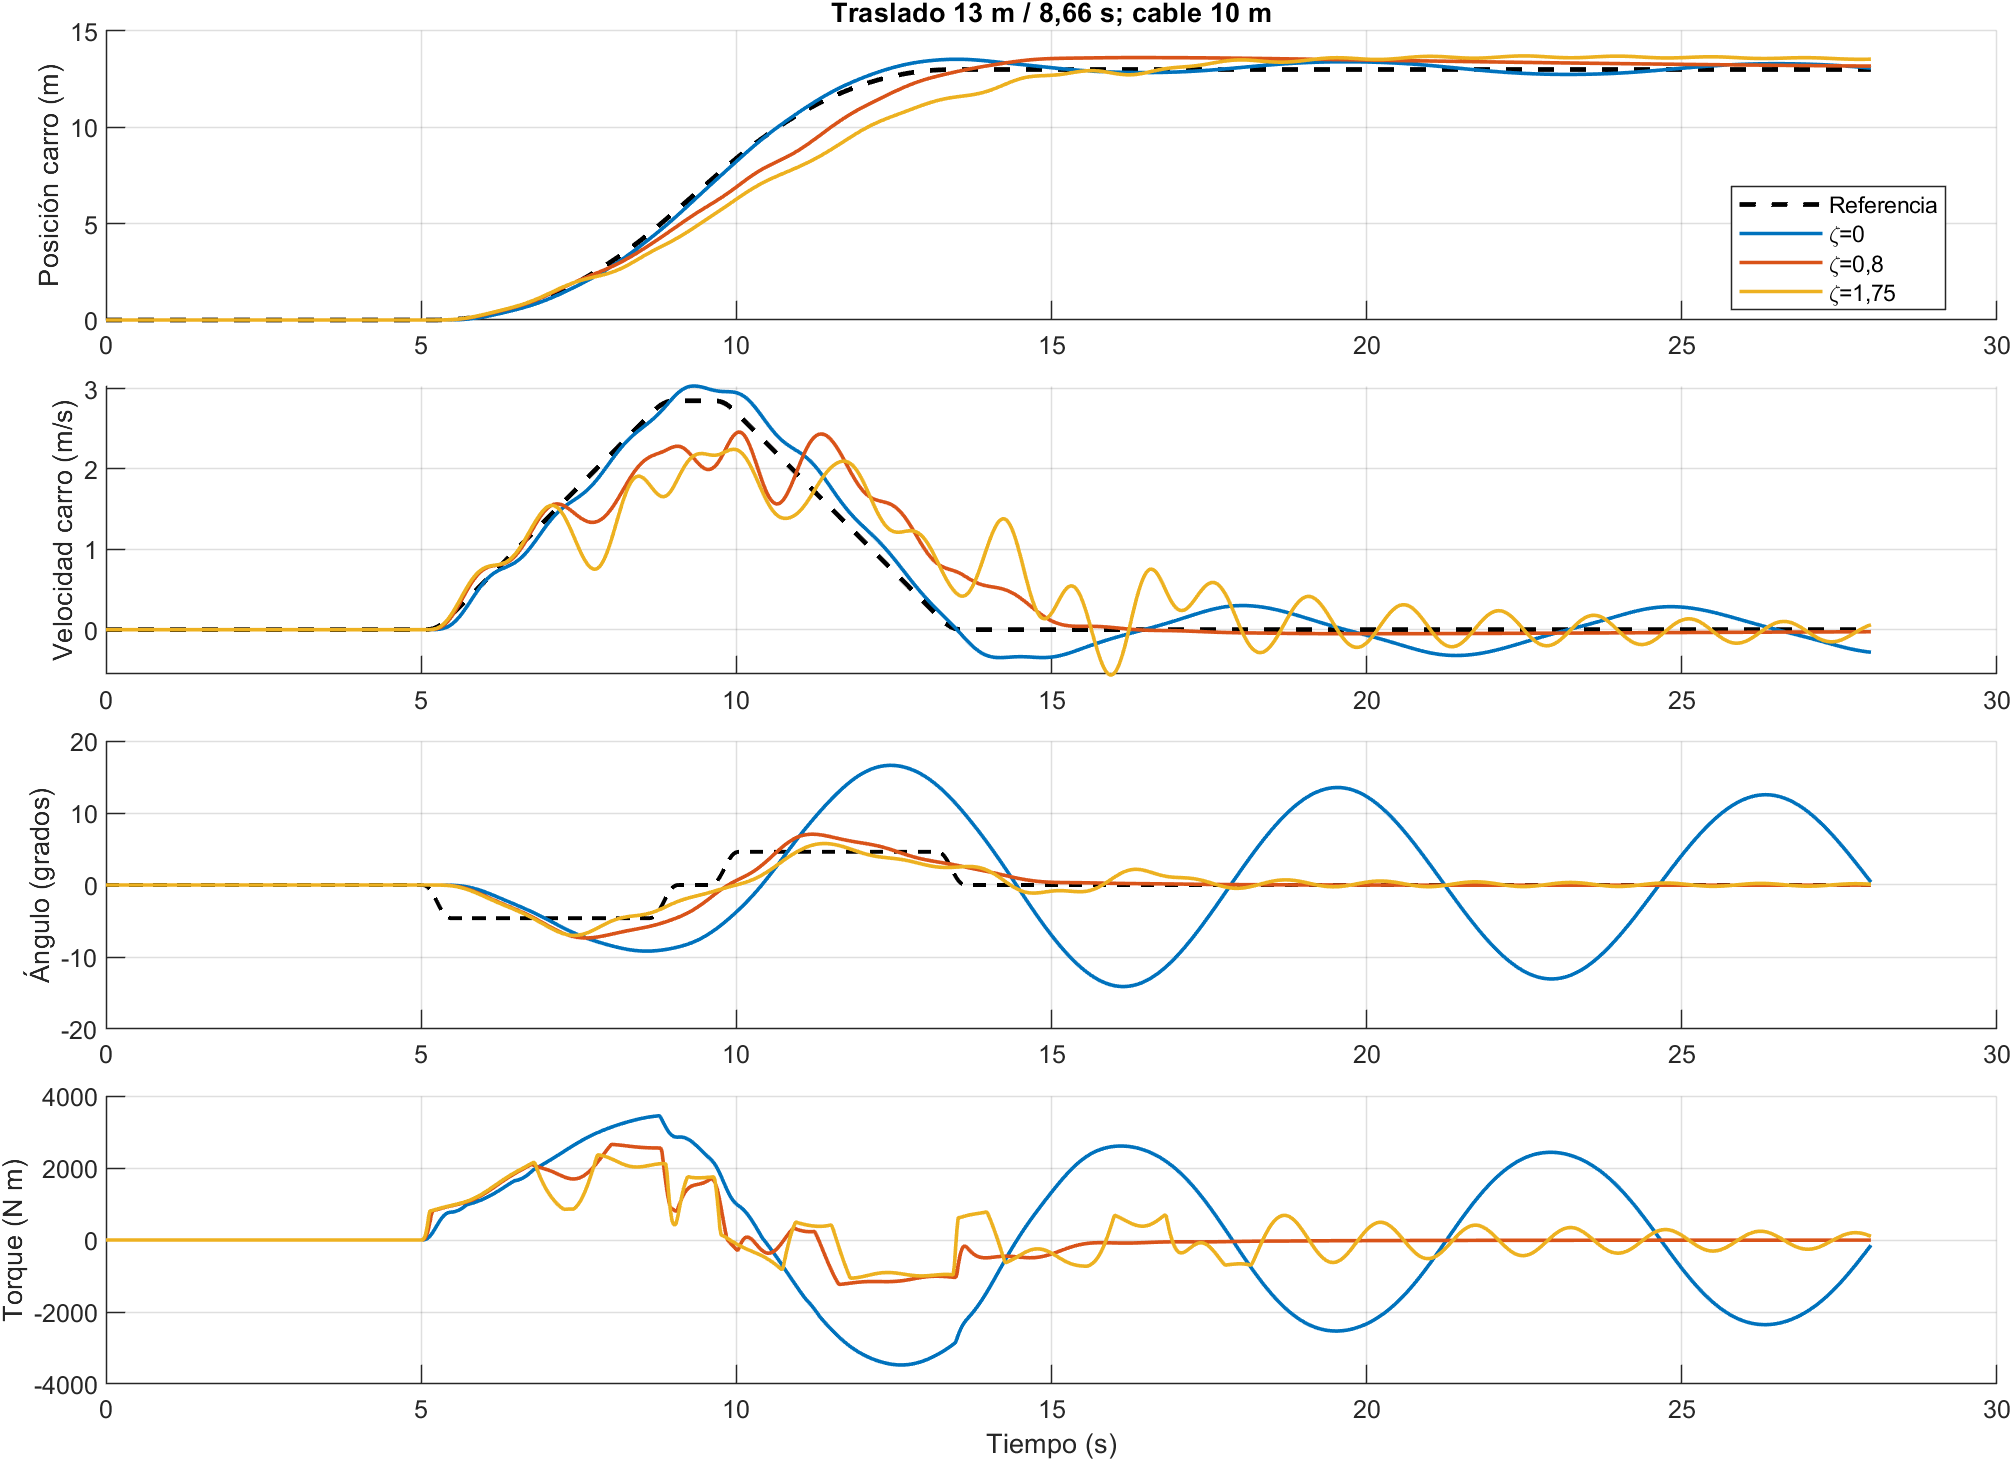
\includegraphics[width=0.82\linewidth]{imagenes_informe/usuario/ensayos_regulatorios_aislados/carro_13m_rapido.png}
		\caption{Traslado rápido: referencias y medidas de posición y velocidad, ángulo y torque.}
		\label{fig:traslado-rapido}
	\end{figure}
	
	\Needspace{5\baselineskip}
	
	\subsubsection{Dos pruebas dirigidas de asignación de polos del carro}
	Primero se conservó el polo integral $p_i=-0,0864~\mathrm{s^{-1}}$ y se aumentó la rapidez del polo principal del PI en tres pasos hasta $p_f=-3,5~\mathrm{s^{-1}}$, con $\zeta_{sw}=1,75$ fijo. La tabla~\ref{tab:polo-rapido} muestra que la ganancia de separación frente a $\omega_p\simeq0,700~\mathrm{rad/s}$ tuvo efecto angular pequeño. El menor ángulo instantáneo al llegar se acompañó de mayor velocidad angular y mayor RMS posmovimiento.
	\begin{table}[H]
		\centering\small
		\caption{Variación del polo rápido en el traslado de 13~m.}
		\begin{tabular}{rrrrr}
			\toprule
			$p_f$ (s$^{-1}$) & $K_{pv}$ & $K_{iv}$ & RMS angular ($^\circ$) & RMS tras llegar ($^\circ$)\\
			\midrule
			$-2,314$ & 2,400 & 0,200 & 0,10507 & 0,01140\\
			$-2,700$ & 2,786 & 0,233 & 0,10465 & 0,01168\\
			$-3,100$ & 3,186 & 0,268 & 0,10446 & 0,01194\\
			$-3,500$ & 3,586 & 0,303 & 0,10440 & 0,01230\\
			\bottomrule
		\end{tabular}
		\label{tab:polo-rapido}
	\end{table}
	La segunda prueba conservó $p_f=-2,314~\mathrm{s^{-1}}$ y desplazó el integral a $p_i=-0,17~\mathrm{s^{-1}}$, para separarlo del lazo externo $K_x=0,05~\mathrm{s^{-1}}$. Resultan $K_{pv}=2,4836~\mathrm{s^{-1}}$ y $K_{iv}=0,3933~\mathrm{s^{-2}}$. Frente a la base, el RMS angular durante movimiento bajó $0,10507\to0,10270^\circ$ y el posterior a la llegada $0,01140\to0,01057^\circ$; el RMS del carro subió $0,16684\to0,16766$~m y el torque máximo pasó de 524,2 a 523,0~Nm. Tampoco actuaron los límites de aceleración ni torque. La mejora de 2,3\% en movimiento es modesta y requiere comprobación en otras condiciones.
	\begin{figure}[H]
		\centering
		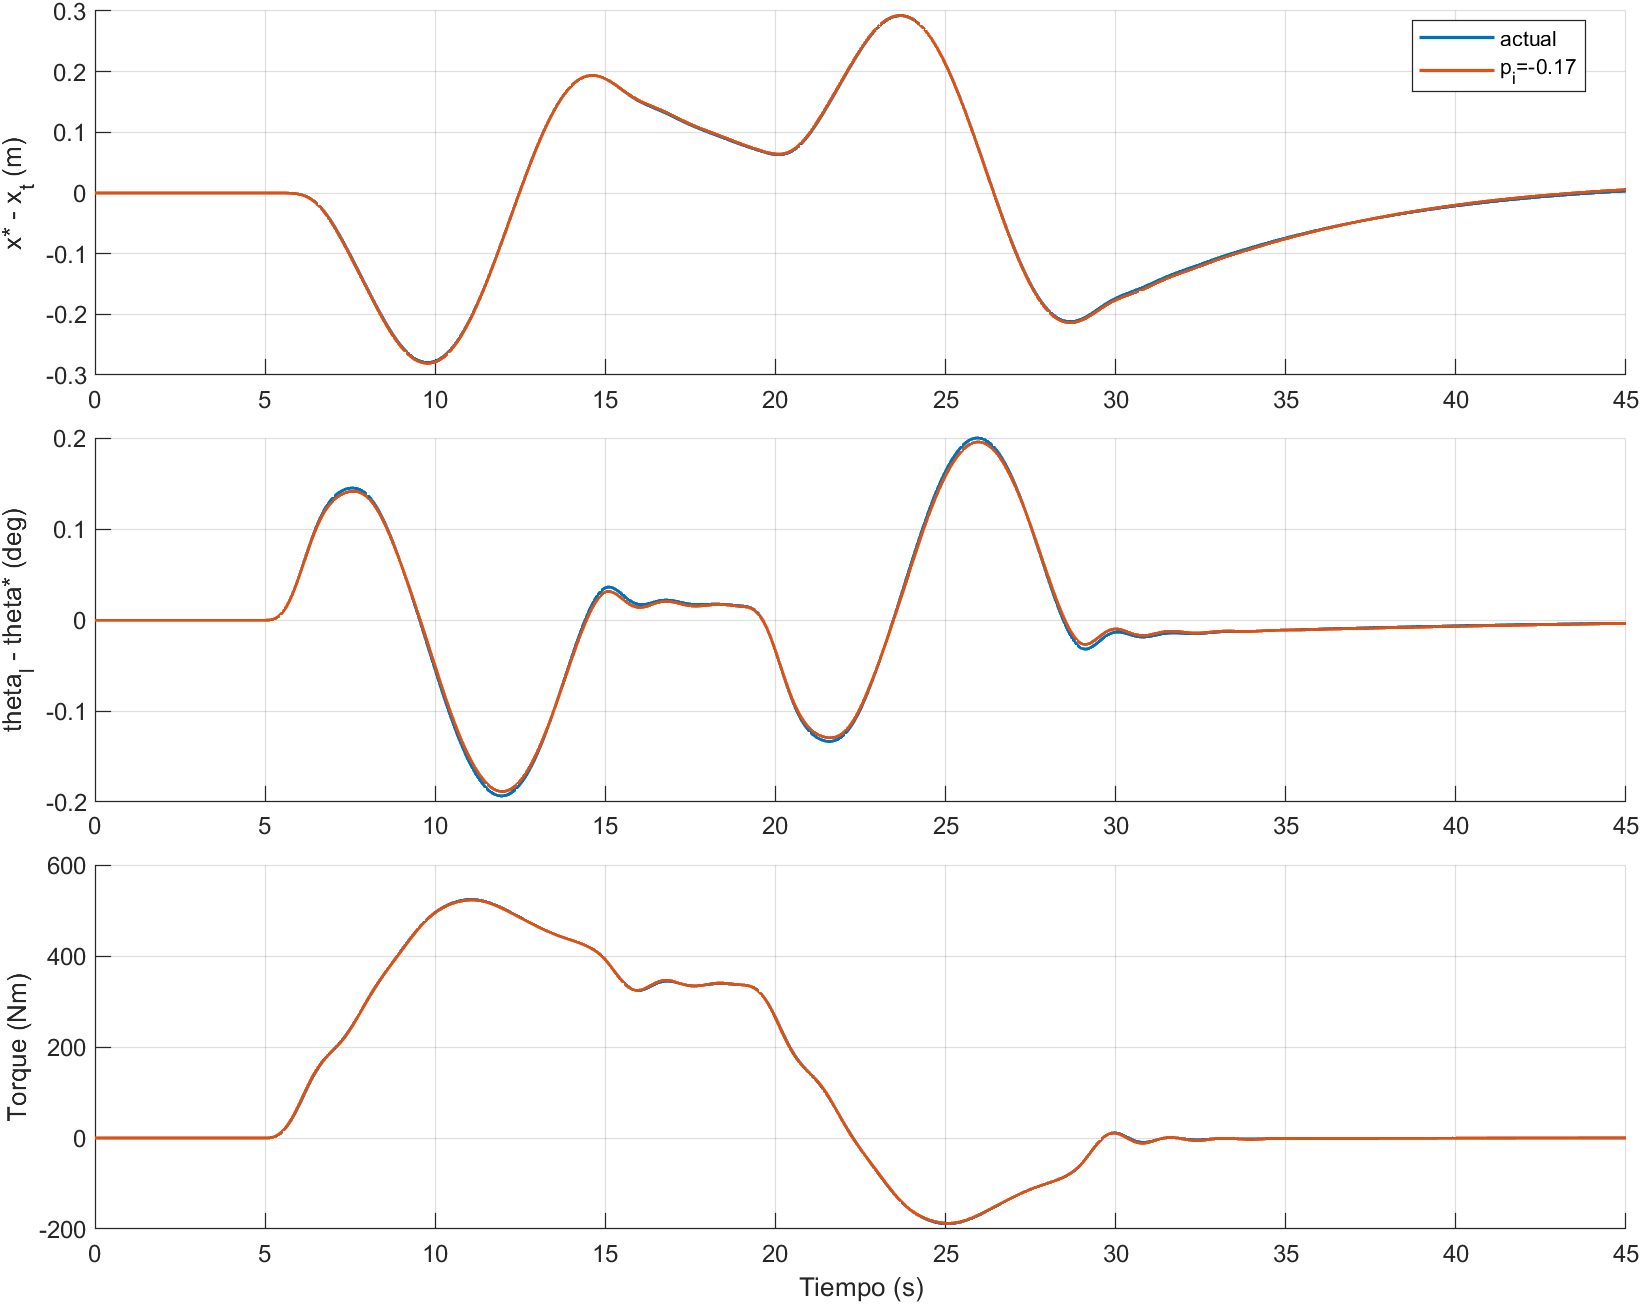
\includegraphics[width=0.62\linewidth]{imagenes_informe/usuario/ensayos_regulatorios_aislados/comparacion_polo_integral.png}
		\caption{Error del carro, error angular y torque para la asignación integral original y la candidata.}
		\label{fig:polo-integral}
	\end{figure}
	
	Estas conclusiones corresponden a bancos aislados. En las 24 corridas nuevas de carro y decaimiento no hubo cuerda floja ni saturación de torque, pero una corrida completada o un RMS bajo no prueban por sí mismos despeje seguro ni una mejora en la maniobra completa. La candidata del polo integral y las asignaciones anti-sway requieren evaluación durante el medio ciclo antes de cambiar la sintonía del modelo integrado.
	
	\paragraph{Ubicación nominal de los polos.}
	Para la cascada ideal, la combinación de \eqref{eq:polos-carro} con el lazo exterior de posición produce
	\begin{equation}
		P_{xv}(s)=s^3+K_{pv}s^2+(K_{iv}+K_xK_{pv})s+K_xK_{iv}.
	\end{equation}
	El modelo pendular usado para asignar el anti-sway tiene $P_{sw}(s)=s^2+2\zeta_{sw}\omega_p s+\omega_p^2$, con $\omega_p=\sqrt{g/l}$. La figura~\ref{fig:polos-regulatorios} ubica los polos nominales de la cascada base y de la candidata integral, y los del péndulo ideal para $l=10$ y 20~m. No son polos identificados de la planta no lineal con límites activos.
	\begin{figure}[H]
		\centering
		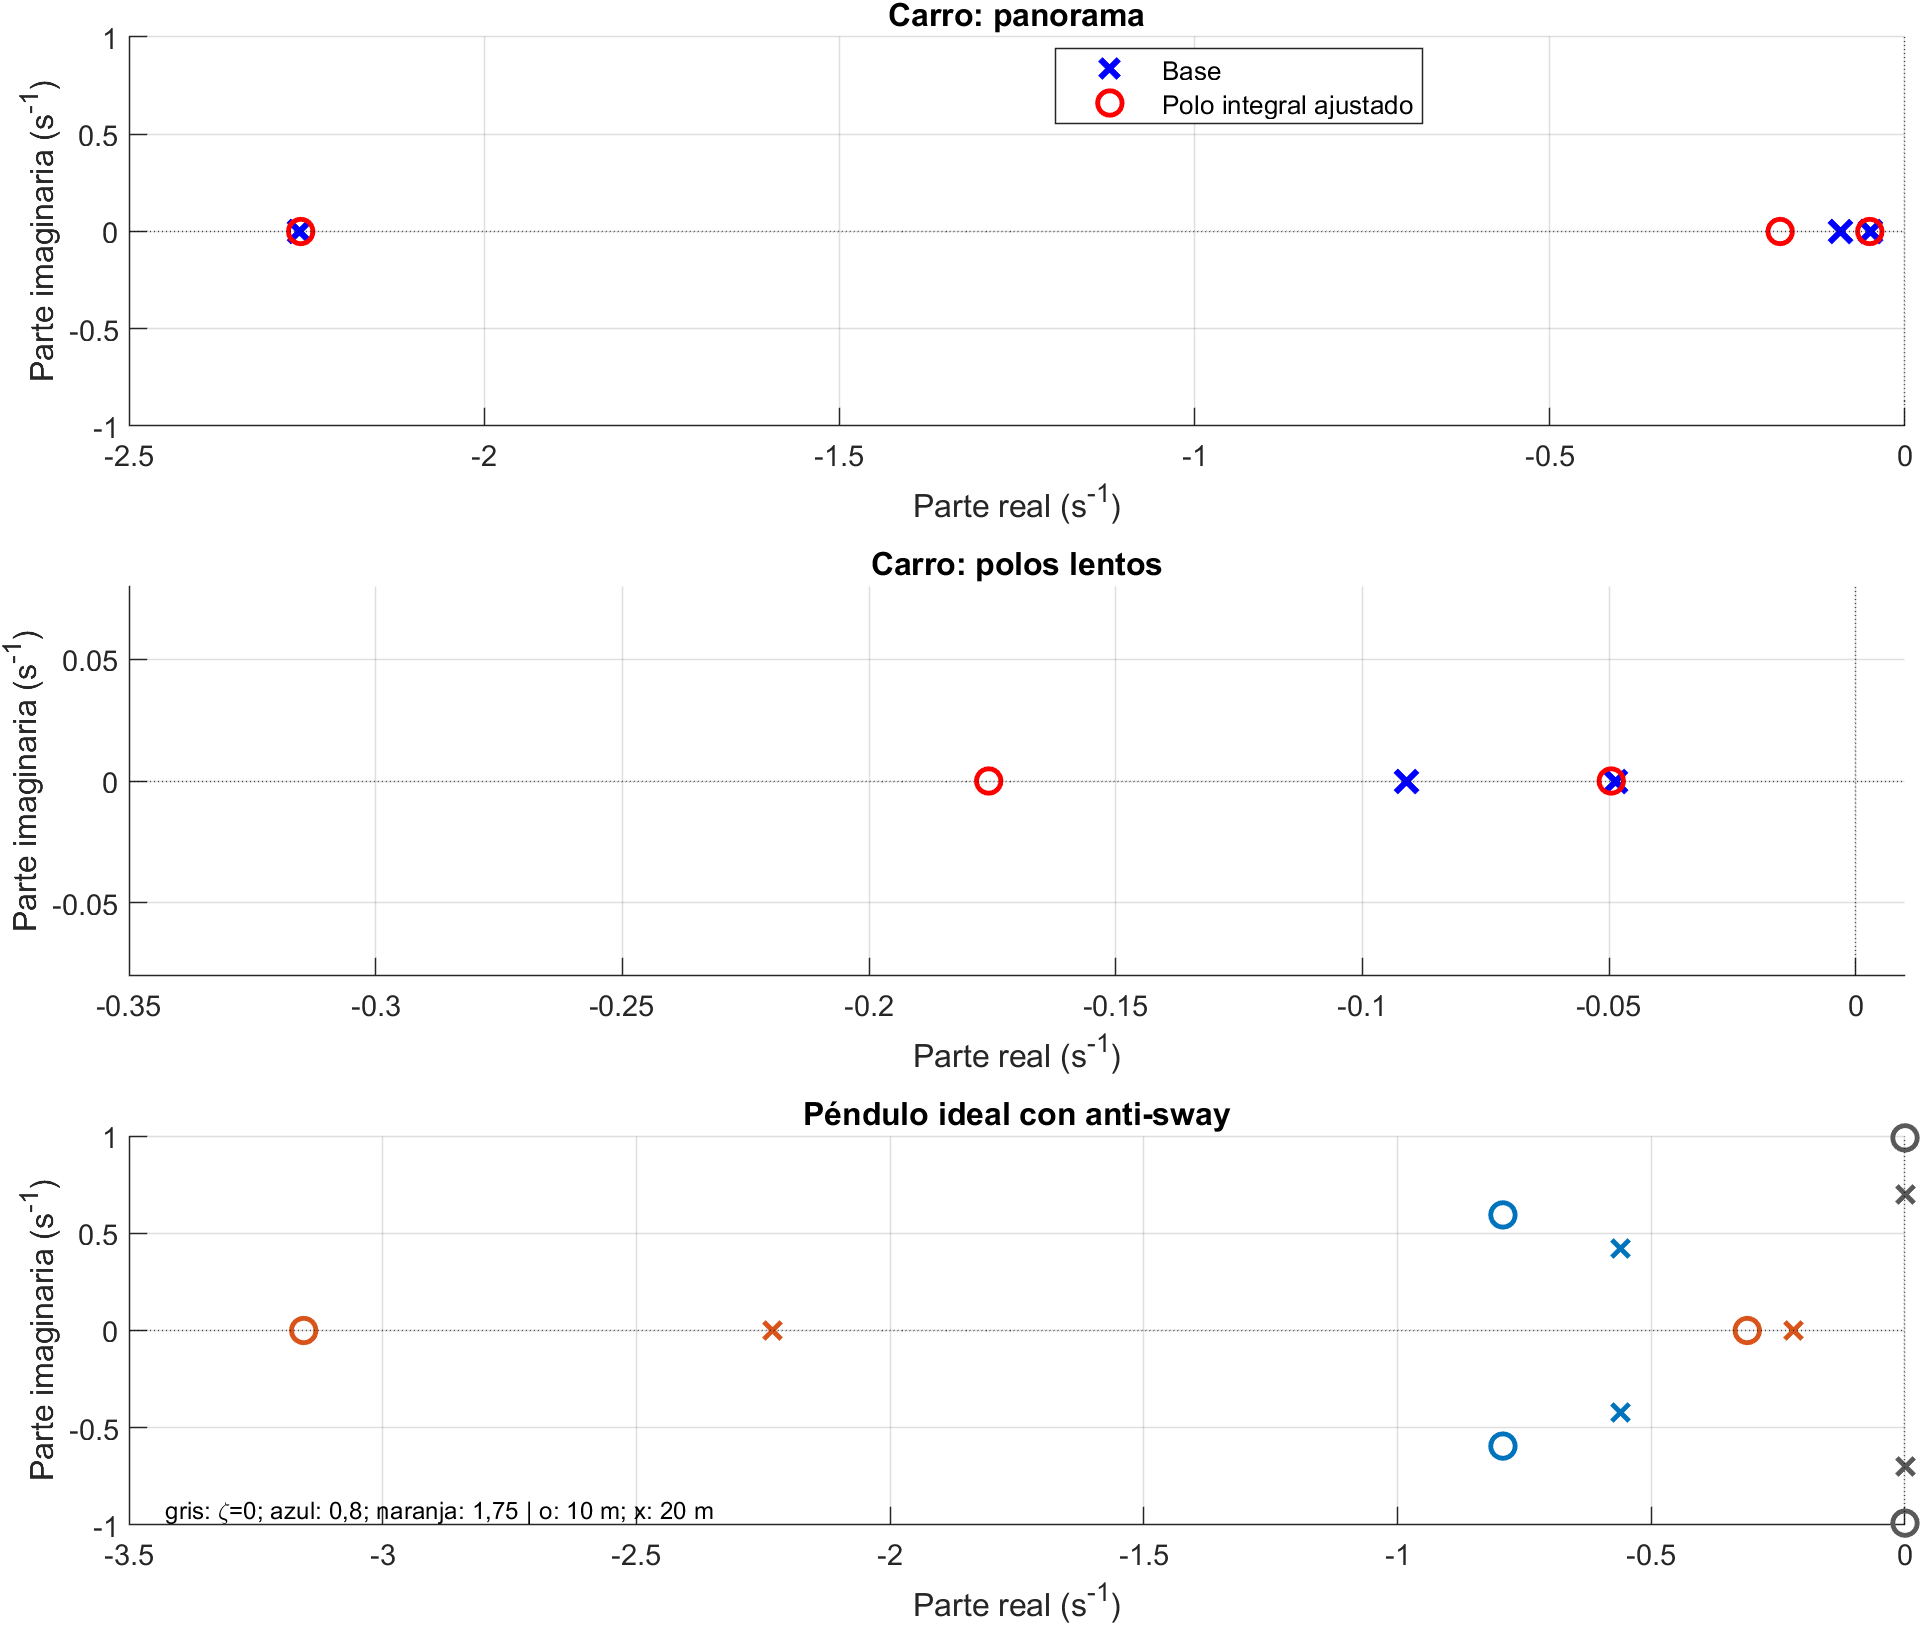
\includegraphics[width=\linewidth]{imagenes_informe/usuario/ensayos_regulatorios_aislados/polos_carro_antisway.png}
		\caption{Polos de diseño del carro y del anti-sway. En el péndulo: gris, $\zeta_{sw}=0$; azul, $0,8$; naranja, $1,75$. Los círculos indican 10~m y las cruces 20~m.}
		\label{fig:polos-regulatorios}
	\end{figure}
	
	\Needspace{5\baselineskip}
	
	\subsubsection{Balance de la sintonía y alcance de los ensayos regulatorios}

Los ensayos aislados permitieron caracterizar el seguimiento y el balanceo bajo condiciones comparables. El izaje siguió los perfiles ensayados con y sin contenedor, sin cuerda floja ni saturación de torque durante el movimiento. En el carro, las modificaciones de polos produjeron mejoras angulares pequeñas frente a la sintonía base.

El compromiso del antisway dependió de la tarea: la asignación $\zeta_{sw}=0{,}8$ favoreció la recuperación desde una perturbación angular inicial, mientras que $\zeta_{sw}=1{,}75$ redujo más el error angular durante el traslado suave, a costa de un mayor error de posición. El traslado rápido mostró que la actuación prolongada del límite de aceleración deteriora el seguimiento y condiciona las referencias admisibles.

Estos resultados orientan la sintonía y la suavidad de las trayectorias. La coordinación de los ejes, el despeje de obstáculos y las transferencias entre modos se evalúan posteriormente con el sistema integrado.
\Needspace{5\baselineskip}

\subsection{Integración de los sistemas durante la maniobra completa}
Los ensayos con referencias aisladas permiten evaluar el seguimiento, la amortiguación del balanceo y la sintonía de los reguladores bajo condiciones definidas. La maniobra completa agrega cambios de objetivo y fases consecutivas: barrido, aproximación manual, toma de carga, traslado automático, descarga y retorno. Cada fase comienza con los estados físicos que deja la anterior. Por ello, la integración requiere comprobar también las transiciones y las maniobras manuales, además de las ventanas de traslado automático.

\textbf{Ensayo de la integración original y etapas de la maniobra.} El ensayo comienza con el spreader vacío. Primero se habilita el sistema y se releva el perfil; luego se aproxima manualmente al contenedor del muelle. Tras el contacto se cierran los twistlocks y se eleva la carga hasta habilitar el traslado automático al barco. Allí se realiza la descarga manual; el spreader vacío se eleva y retorna automáticamente al muelle. El retorno concluye con la parada, sin un descenso final para tomar otra carga.

Los eventos registrados permiten agrupar la maniobra en ocho fases:

\begin{table}[H]
\centering
{\small
\begin{tabular}{@{}L{0.25\textwidth}L{0.22\textwidth}L{0.45\textwidth}@{}}
\toprule
Fase & Intervalo [s] & Desarrollo\\
\midrule
I. Arranque y barrido & 0,000--106,600 & Habilitación, elevación inicial y recorrido para relevar el perfil.\\
II. Aproximación manual & 106,600--203,000 & Descenso vacío, desplazamiento horizontal con joystick, retirada y ajustes hasta el contacto.\\
III. Toma y elevación & 203,000--232,400 & Cierre de twistlocks, confirmación de carga y elevación previa al traslado.\\
IV. AUTO cargado & 232,400--296,400 & Traslado al destino del barco siguiendo las referencias automáticas.\\
V. Descarga manual & 296,400--332,400 & Paso a manual, descenso hasta el contacto y liberación del contenedor.\\
VI. Elevación vacía & 332,400--355,600 & Elevación del spreader y preparación del retorno.\\
VII. AUTO vacío & 355,600--392,600 & Retorno horizontal al muelle sin descenso final.\\
VIII. Parada & 392,600--393,799 & Orden de parada y confirmación de reposo.\\
\bottomrule
\end{tabular}
}
\end{table}

Estas fases agrupan eventos del operador y del supervisor para interpretar el ensayo; no sustituyen los estados internos del autómata. En particular, la fase de aproximación manual contiene movimientos, reposos y microajustes sucesivos.


\begin{figure}[H]
\centering
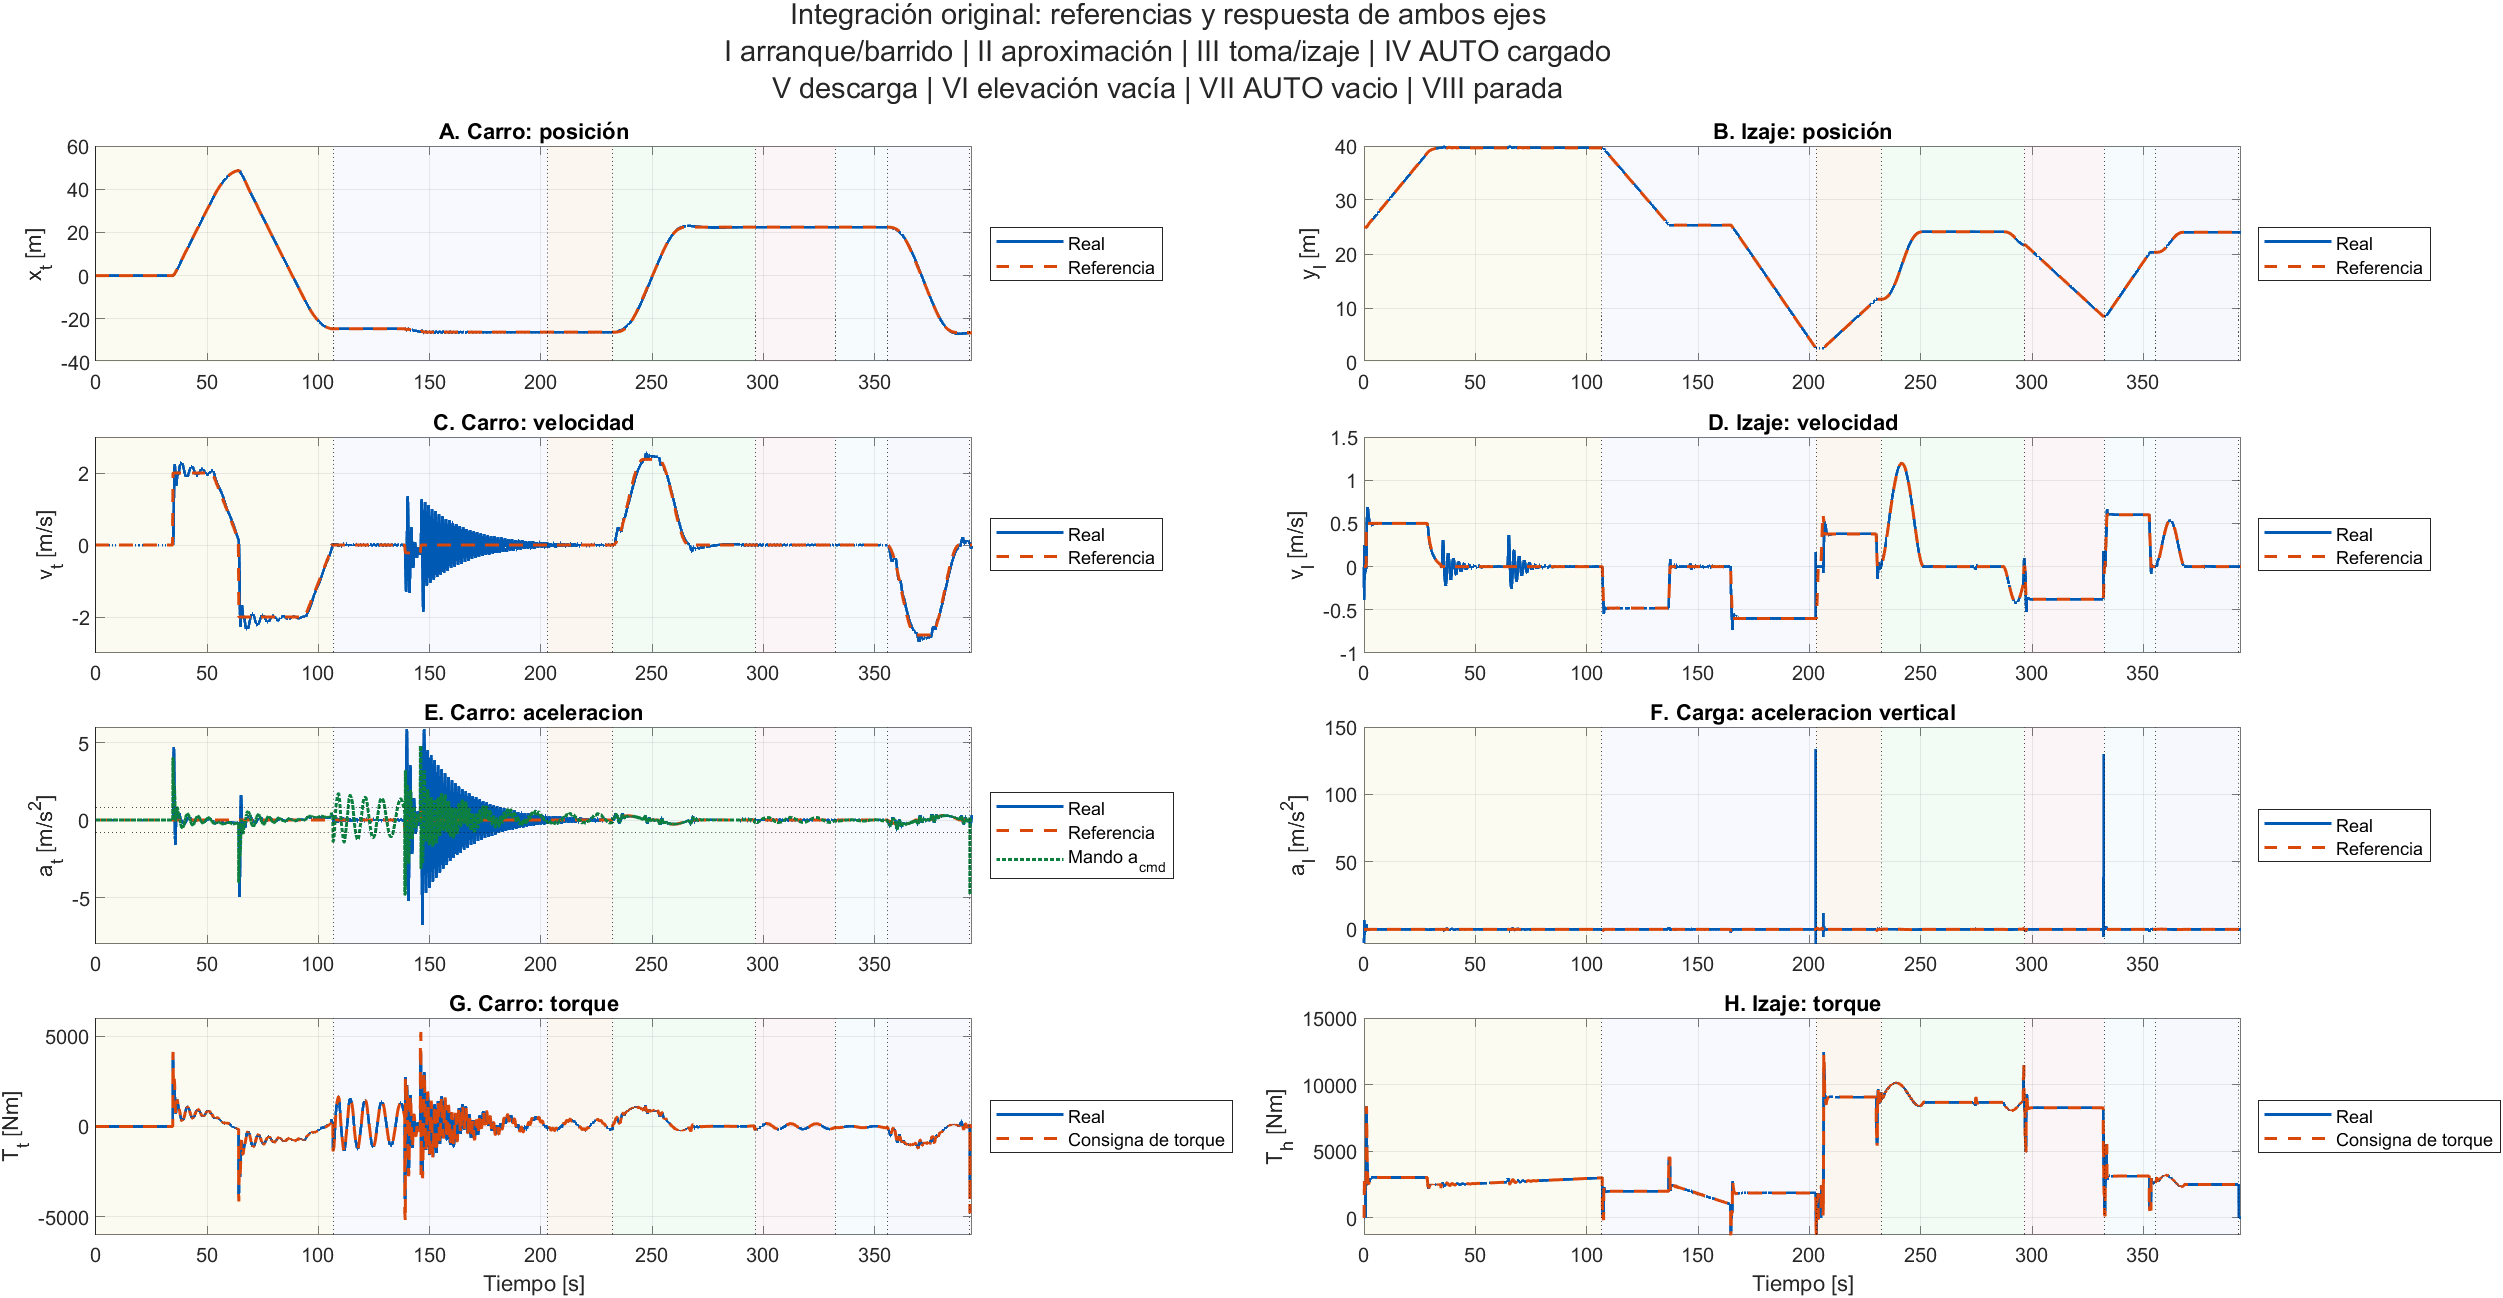
\includegraphics[width=0.99\textwidth,height=0.72\textheight,keepaspectratio]{imagenes_informe/usuario/integracionP1/01_01_ciclo_integracion_original.png}
\caption{Maniobra completa de la integración original. Cuatro filas muestran posición, velocidad, aceleración y torque; la columna izquierda corresponde al carro y la derecha al eje vertical. Azul: respuesta física; naranja discontinua: referencia o consigna de torque del controlador. Verde punteada en E: mando de aceleración del carro. Los fondos y las divisiones verticales identifican las fases I--VIII de la tabla. La aceleración vertical corresponde a la carga y conserva los transitorios de arranque y contacto. Las referencias de posición deben interpretarse junto con las de velocidad: en manual, el objetivo del operador es de velocidad y la posición sirve a la gestión de retención.}
\label{fig:integracion_p1_1}
\end{figure}

\textbf{Resultado general de la integración y evaluación de los traslados automáticos.} La integración mostró resultados favorables: la maniobra terminó en \textbf{393,799 s}, sin aborto, y el supervisor coordinó el barrido, la intervención manual, la toma y entrega de carga y los dos traslados automáticos. En particular, los recorridos automáticos cargado y vacío mantuvieron un buen seguimiento de las referencias, demandas de velocidad y torque dentro de los límites evaluados y un balanceo reducido al llegar. Sus duraciones fueron \textbf{64,0 s} y \textbf{37,0 s}, respectivamente.

Para evaluar este desempeño se separan las ventanas AUTO cargado y AUTO vacío. Sobre ellas se contrastan las referencias con la respuesta física y se comprueban tres aspectos principales:

\begin{itemize}
\item \textbf{Posición y seguimiento:} se compara la trayectoria de cada eje con su referencia, distinguiendo los errores durante el recorrido del error al alcanzar el destino. El máximo error vertical en AUTO fue \textbf{59,7 mm} y el máximo error horizontal transitorio fue \textbf{0,621 m}. Este último no es el error final de posicionamiento: al terminar el ciclo, el carro quedó a \textbf{0,228 m} del destino del muelle, dentro de la banda de aceptación de \textbf{0,35 m}. El evaluador comprueba explícitamente el seguimiento vertical y la posición final de retorno; no utiliza el máximo error horizontal transitorio como uno de sus criterios binarios.
\item \textbf{Velocidad:} se comprueba que la velocidad física y la referencia respeten los límites de cada eje. Para izaje, el límite de referencia depende de la masa y de la región de potencia constante. En AUTO, la velocidad máxima del carro fue \textbf{2,691 m/s}; la velocidad vertical máxima fue \textbf{1,194 m/s} con carga y \textbf{0,533 m/s} en vacío. La estimación de masa y las referencias también aprobaron sus comprobaciones.
\item \textbf{Torque y capacidad del accionamiento:} se verifica que las demandas puedan ser aplicadas por los motores y que el accionamiento de izaje respete la evaluación de potencia. Los máximos físicos durante AUTO fueron \textbf{1,206 kNm} en el carro y \textbf{10,123 kNm} en izaje, inferiores a los límites nominales de \textbf{4 y 20 kNm}. La potencia mecánica máxima de izaje fue \textbf{697,9 kW}.
\end{itemize}

La evaluación se completa con aceleración, balanceo, tensión del cable, estado de los frenos y ausencia de fallas. Las aceleraciones máximas evaluadas durante AUTO fueron aproximadamente \textbf{0,628 m/s\textsuperscript{2}} para el carro y \textbf{0,323 m/s\textsuperscript{2}} para la carga; el ángulo en crucero no superó \textbf{0,358\ensuremath{^{\circ}}} y fue menor a \textbf{0,1\ensuremath{^{\circ}}} en los eventos de llegada.

Estos resultados respaldan el desempeño de los traslados automáticos en la maniobra ensayada. En la vista global destaca la oscilación del carro durante la aproximación manual. El primer caso que se analiza a continuación aparece al retirar el joystick dentro de esa etapa, y permite estudiar cómo una orden manual excita la dinámica de la planta.

\Needspace{5\baselineskip}

\subsection{Detección del pico durante la parada manual}
En la maniobra inicial se reprodujo un pico de aceleración física de \textbf{-6,7643 m/s\textsuperscript{2}} después de retirar el joystick horizontal. El evento se reconstruyó con las señales internas del control y con la salida de aceleración de la planta.



\begin{table}[H]
\centering
{\small
\begin{tabular}{@{}L{0.64\textwidth}L{0.30\textwidth}@{}}
\toprule
Instante & Observación\\
\midrule
145,800 s & Se retira el joystick. La referencia angular pasa a aproximadamente -0,0814 rad.\\
Desde 145,800 s & La corrección anti-sway alcanza +3,2 m/s y el torque del carro permanece en el límite positivo de 4000 Nm durante aproximadamente 0,28 s.\\
146,080 s & El ángulo de referencia vuelve a cero. La corrección anti-sway cambia bruscamente y el torque solicitado invierte su signo.\\
146,7437 s & La aceleración física alcanza -6,7643 m/s\textsuperscript{2}, después del pulso de mando y de su inversión.\\
\bottomrule
\end{tabular}
}
\end{table}

Esto indica que el salto de corrección se originaba principalmente en la referencia angular, aun cuando el ángulo físico era pequeño. La cadena de eventos que lo explican:
Soltar el joystick \(\rightarrow\) pulso de aceleración de referencia \(\rightarrow\) cambio brusco de $\theta_{ref}$ \(\rightarrow\) corrección anti-sway grande \(\rightarrow\) pulso de torque \(\rightarrow\) deformación de la transmisión \(\rightarrow\) pico posterior de aceleración del carro.



\begin{figure}[H]
\centering
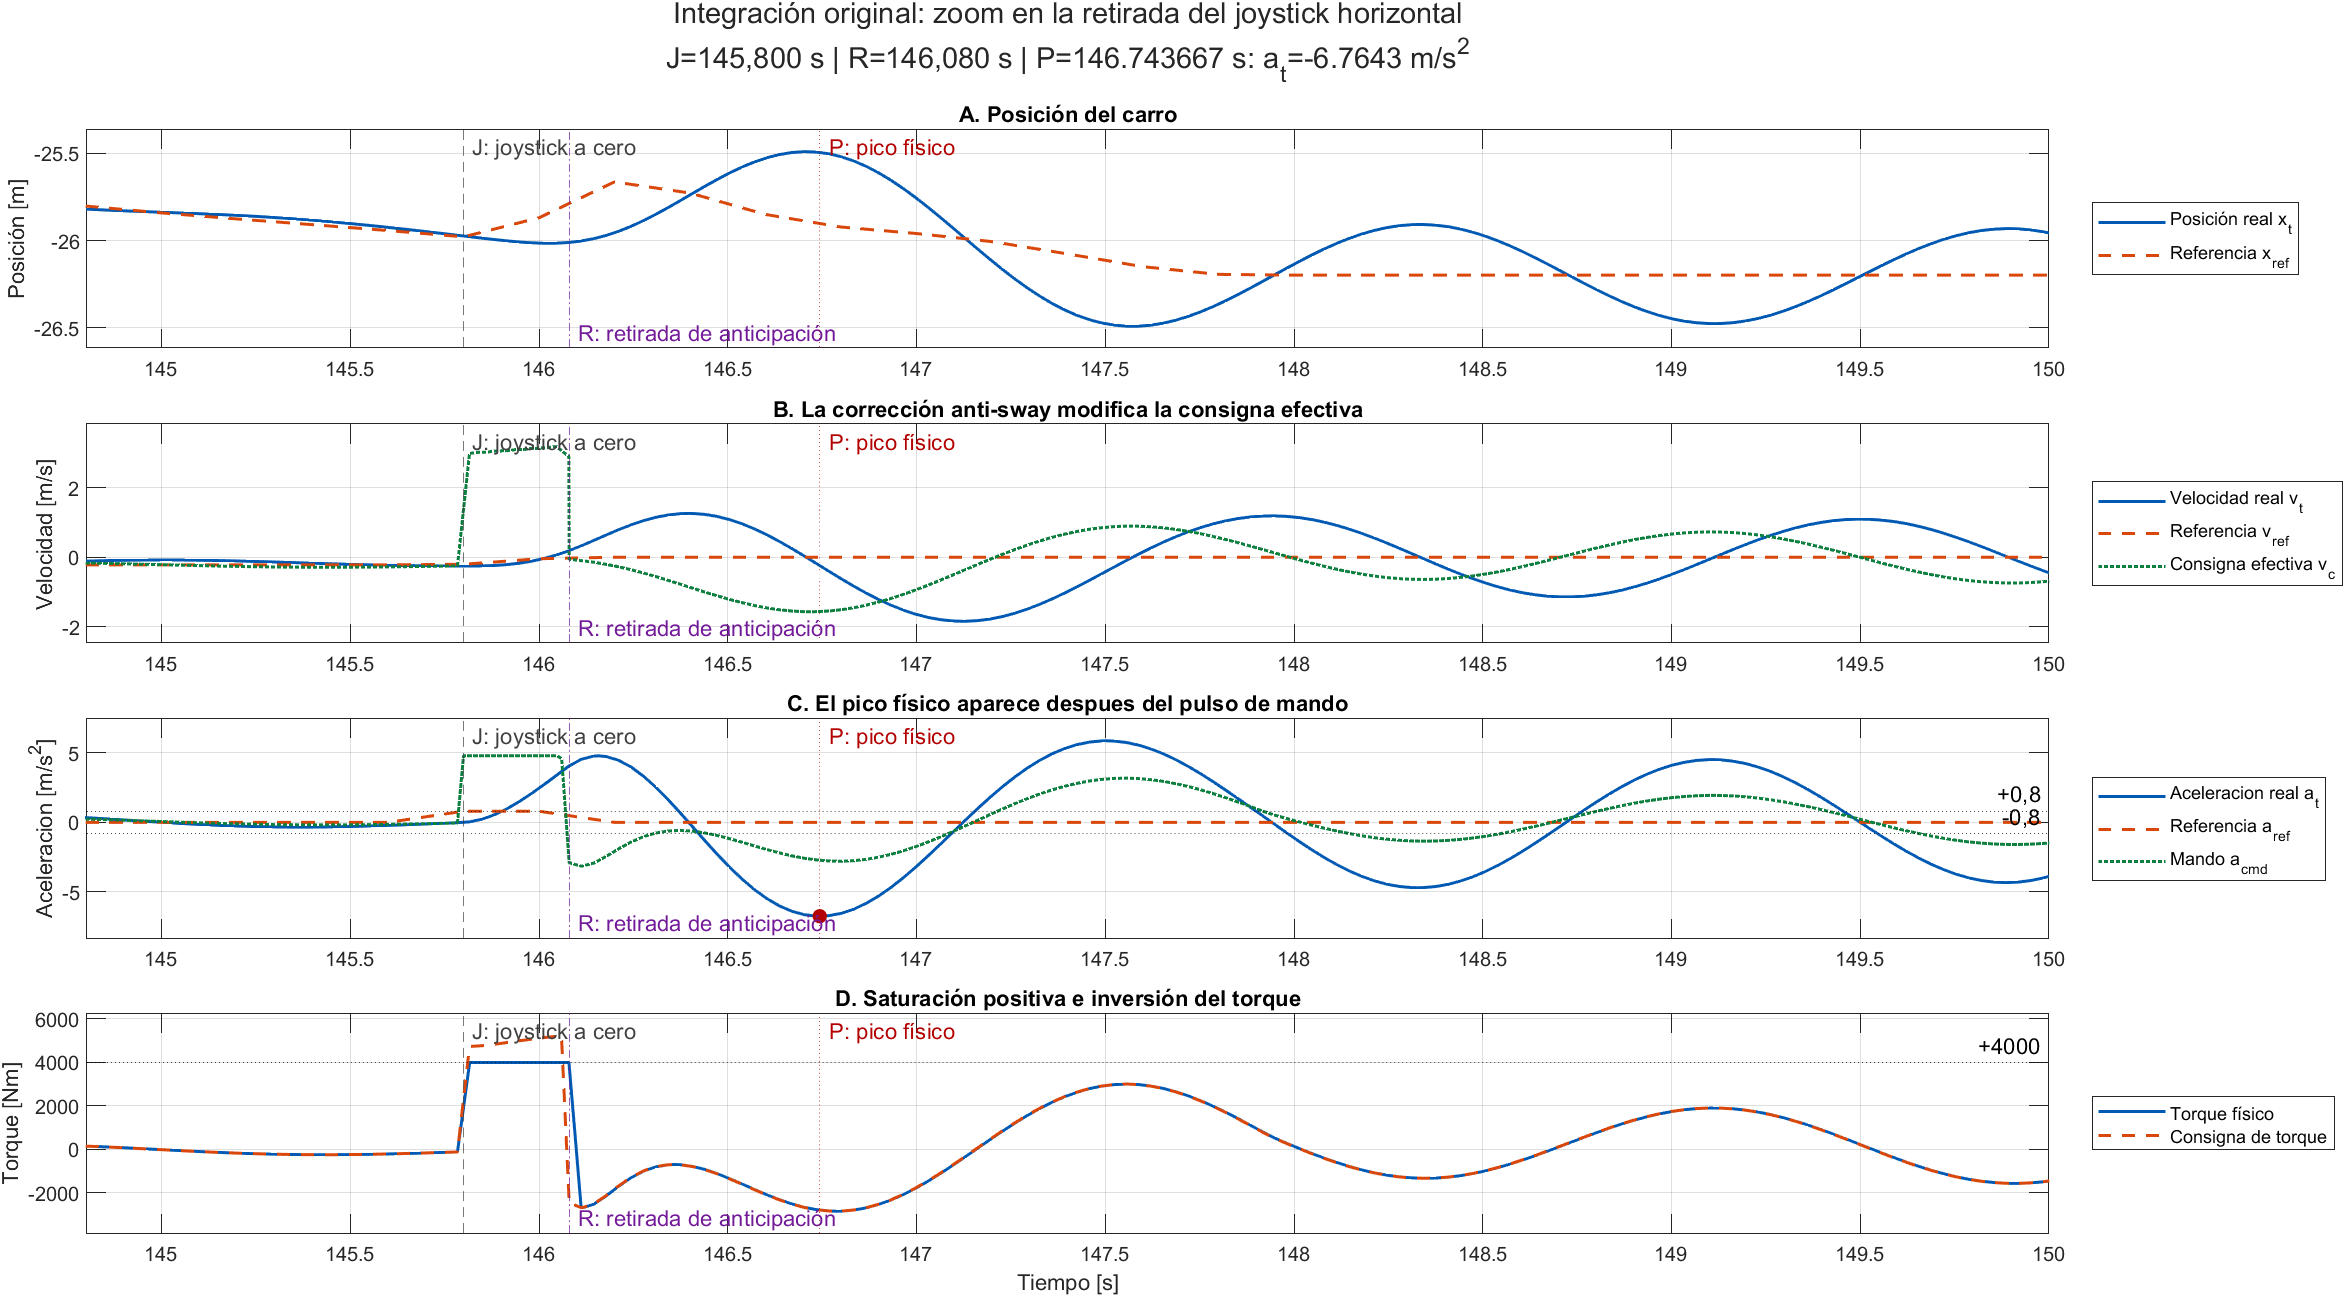
\includegraphics[width=0.99\textwidth,height=0.72\textheight,keepaspectratio]{imagenes_informe/usuario/integracionP1/02_02_zoom_retirada_joystick.png}
\caption{Detalle del carro entre 144,8 y 150 s. A: posición y referencia. B: velocidad física, referencia nominal y consigna efectiva que incorpora la corrección anti-sway. C: aceleración física, referencia y mando regulatorio. D: consigna de torque y torque físico del motor. J, gris discontinua, marca la retirada del joystick a 145,800 s; R, violeta, la retirada de la anticipación a 146,080 s; P, roja punteada, el pico físico a 146,743667 s. Las cotas \(\pm\)0,8 m/s\textsuperscript{2} representan el criterio cinemático adoptado; en esta versión original el mando total todavía puede superarlo. El drive recorta el torque a \(\pm\)4000 Nm.}
\label{fig:integracion_p1_2}
\end{figure}

El zoom permite distinguir el origen del evento y su respuesta posterior. La referencia nominal de velocidad se aproxima a cero al soltar el joystick, pero la consigna efectiva aumenta por la corrección anti-sway. El regulador produce entonces un pulso de aceleración y de torque; al retirarse la anticipación, el torque cambia de signo. El carro continúa oscilando por la dinámica elástica y alcanza el máximo negativo después de esa inversión. Se reproduce así el pico original, sin atribuirlo a una orden adicional de desplazamiento del operador.
La primera solución combinó tres medidas.

\textbf{1. Filtro de retardo en la señal analógica del joystick.}
La conexión y lectura de los ejes analógicos de un joystick de PlayStation se probaron físicamente. Para suavizar los cambios de su objetivo de velocidad se incorporó un filtro de retardo entre $v_{nom}$ y la referencia que recibe el control. El filtro es de segundo orden críticamente amortiguado, con $\omega_n=0,50$ rad/s, y suministra conjuntamente velocidad y aceleración coherentes. Al soltar el analógico, el objetivo vuelve a cero y la referencia completa gradualmente la desaceleración. Esto reduce el pulso que cambia la referencia angular y excita el anti-sway, a costa de un recorrido residual que debe considerarse al detenerse. La mejora cuantificada corresponde al ensayo simulado de la planta; la prueba física verifica la conexión del joystick.

\textbf{2. Límite de la acción PI durante la maniobra manual.} Se redujo la contribución máxima del PI a \textbf{\(\pm\)0,25 m/s\textsuperscript{2}} en manual:

\begin{equation}
a_{PI}=\operatorname{sat}_{0,25}(K_{pv}e_v+K_{iv}I).
\end{equation}

Se conservaron las ganancias y el estado integral, y se obtuvo una reducción de la excitación de la transmisión.

\textbf{3. Límite de pendiente de la velocidad nominal durante el barrido.} Se aplicó una pendiente máxima de \textbf{\(\pm\)0,25 m/s\textsuperscript{2}} a la referencia de velocidad del barrido de perfil para suavizar sus cambios de recorrido. Esto redujo el máximo físico de esa fase de aproximadamente \textbf{4,965 a 0,285 m/s\textsuperscript{2}}. La corrección también cambió el estado final previo a la manipulación manual; por eso las tres medidas se validaron conjuntamente desde el inicio del ciclo.

Con la combinación seleccionada, el máximo absoluto de aceleración física del carro en el ciclo completo pasó de \textbf{6,764 a 0,782 m/s\textsuperscript{2}}. El nuevo máximo ocurrió durante el inicio de la maniobra manual, no en la parada que había originado el diagnóstico. La duración total aumentó aproximadamente 2,2 s, y el resultado demostró la mejora de la combinación para las condiciones ensayadas.


Esta primera combinación corresponde a la variante A14. En el diseño posterior se utilizaron referencias comunes con aceleración nominal de 0,3 m/s\textsuperscript{2} y jerk de 0,5 m/s\textsuperscript{3}, y un límite de \(\pm\)0,8 m/s\textsuperscript{2} sobre la suma total de aceleraciones. El límite PI específico de manual de esta primera etapa no se conserva como una selección por modo en el controlador común que se analiza a continuación.

\Needspace{5\baselineskip}

\subsection{Por qué la aceleración física puede superar a la comandada}
El regulador utiliza el modelo reducido del carro para convertir aceleración en torque. Ese modelo aproxima el movimiento del tambor y del carro mediante una misma coordenada. La planta completa conserva la elasticidad de la transmisión:

\begin{equation}
F_{tw}=K_{tw}(x_{td}-x_t)+b_{tw}(\dot x_{td}-\dot x_t),
\end{equation}

\begin{equation}
\ddot x_t=\frac{F_{tw}+2F_{hw}\sin\theta_l-b_t\dot x_t}{M_t}.
\end{equation}

Por tanto, la aceleración física depende de la fuerza transmitida por el cable y de los estados relativos entre tambor y carro. Un pulso de torque puede aumentar la deformación y almacenar energía elástica,

\begin{equation}
U_{tw}=\frac12 K_{tw}(x_{td}-x_t)^2,
\end{equation}

que se libera posteriormente. El máximo físico puede aparecer después del máximo de mando y cuando el torque ya no está saturado.

En el diagnóstico inicial, la deformación próxima al pico fue de -0,4128 m. Con una rigidez de 480000 N/m, el esfuerzo elástico asociado resulta del orden de -198 kN. La reducción de la excitación también redujo la energía elástica máxima de la ventana manual: de aproximadamente 40,94 kJ a 0,538 kJ.

\Needspace{5\baselineskip}

\subsection{Anti-windup ante límites de aceleración y de torque}
\label{sec:integracion_aw}

El anti-windup se incorpora como mejora del diseño para maniobras en las que los límites impidan aplicar lo que solicita el PI. Su justificación no depende de que el ciclo nominal final sature el torque. Incluso con una referencia nominal de aceleración moderada, la suma con la respuesta del PI a la corrección de balanceo puede alcanzar el límite de aceleración; además, el torque incluye términos de compensación que pueden llevar al límite del accionamiento.

\Needspace{5\baselineskip}

\subsubsection{Limitación de la suma de aceleraciones}

Sea la consigna efectiva de velocidad

\begin{equation}
v_c=v_{ref}+v_x+v_{sw},\qquad e_v=v_c-\hat v_t,
\end{equation}

donde $v_x$ representa la corrección del lazo de posición. La salida sin limitar es

\begin{equation}
a_u=a_{ref}+K_{pv}e_v+K_{iv}I.
\end{equation}

Se aplica un único límite a esa suma:

\begin{equation}
a_c=\operatorname{sat}_{a_{max}}(a_u),\qquad a_{max}=0,8\ \mathrm{m/s^2},
\end{equation}

con $\operatorname{sat}_L(z)=\min(L,\max(-L,z))$.

La anticipación $a_{ref}$ llega directamente a la suma desde el generador de referencias. El error de recorte es

\begin{equation}
\Delta a_a=a_c-a_u.
\end{equation}

Si el pedido excede el límite positivo, este error es negativo y corrige la acumulación integral en el sentido que reduce el exceso. Si no hay recorte, es cero.

\Needspace{5\baselineskip}

\subsubsection{Conversión paramétrica del recorte de torque}

La ley de torque del modelo reducido puede escribirse como

\begin{equation}
T_u=K_{Ta}\left(a_c+\frac{b_{\mathrm{EQt}}}{M_{\mathrm{EQt}}}\hat v_t
-\frac{2F_{hw}}{M_{\mathrm{EQt}}}\sin\theta_l\right),
\qquad K_{Ta}=\frac{r_{td}M_{\mathrm{EQt}}}{i_t}.
\end{equation}

Para observar la saturación del accionamiento se comparan su entrada real $T_{in}$ y la salida de su limitador $T_{lim}$:

\begin{equation}
T_{lim}=\operatorname{sat}_{T_{max}}(T_{in}),\qquad
\Delta T=T_{lim}-T_{in}.
\end{equation}

El recorte se convierte a aceleración equivalente mediante la inversa de la conversión del regulador:

\begin{equation}
\boxed{\Delta a_T=\frac{i_t}{r_{td}M_{\mathrm{EQt}}}\,\Delta T.}
\end{equation}

El recorte se mide \textbf{antes de la dinámica del motor}. La diferencia entre el torque físico y el limitado incluye el retardo normal del accionamiento y no representa, por sí misma, una saturación.

\Needspace{5\baselineskip}

\subsubsection{Un integrador con dos causas de recorte}

Ambas contribuciones actúan sobre el mismo estado integral. Una formulación dimensional de retrocálculo es

\begin{equation}
\dot I=e_v+\frac{1}{K_{iv}T_{aw}}\left(\Delta a_a+\Delta a_T\right).
\end{equation}

El tiempo de seguimiento del anti-windup es $T_{aw}=1~\mathrm{s}$, y la ganancia de retrocálculo es $1/(K_{iv}T_{aw})$. Con $K_{iv}$ en $\mathrm{s^{-2}}$, esta ganancia tiene unidades de segundos y convierte el recorte de aceleración en una corrección de velocidad. El código ensayado escribe numéricamente \texttt{1/K\_iv\_cas} porque fija implícitamente $T_{aw}=1~\mathrm{s}$. En la implementación ensayada, ambas diferencias llegan con una muestra de demora, $T_s=1$ ms, para evitar el lazo algebraico. Si

\begin{equation}
q[n]=e_v[n]+\frac{\Delta a_a[n-1]+\Delta a_T[n-1]}{K_{iv}T_{aw}},
\end{equation}

la realización trapezoidal ensayada utiliza una salida integral $I[n]$ y una memoria interna $X[n]$, limitadas por separado:

\begin{align}
I[n]&=\operatorname{sat}_{I_{max}}\left(X[n]+\frac{T_s}{2}q[n]\right),\\
X[n+1]&=\operatorname{sat}_{I_{max}}\left(I[n]+\frac{T_s}{2}q[n]\right),
\qquad I_{max}=\frac{a_{max}}{K_{iv}}.
\end{align}

En cada muestra se calcula primero $I[n]$, que alimenta la contribución $K_{iv}I[n]$ del PI, a partir de la memoria $X[n]$ y del primer medio paso de la entrada actual. Luego se actualiza $X[n+1]$ con el segundo medio paso. La condición inicial de la memoria es $X[0]=0$. Esta es la recurrencia que reproduce el bloque Tustin limitado y que se conserva en el código del MC; allí la misma entrada $q[n]$ se denomina $u_I[n]$.

Mientras ninguna de las dos operaciones satura, puede sustituirse $X[n]=I[n-1]+(T_s/2)q[n-1]$ y recuperar la integración trapezoidal habitual. Cuando hay recorte, esa sustitución deja de ser válida: limitar solamente el resultado de un incremento trapezoidal completo no reproduce necesariamente la entrada y salida del límite. Por ejemplo, con la salida y la memoria en el límite superior, una entrada negativa reduce inmediatamente $I[n]$ en el primer medio paso; el valor positivo de la entrada anterior no vuelve a incorporarse explícitamente. Por ello, las dos ecuaciones anteriores describen también el comportamiento durante saturación y deben conservarse para representar la implementación ensayada.

Con $K_{iv}=0,2\ \mathrm{s^{-2}}$, resulta $I_{max}=4$ m. Este límite corresponde al estado que integra el error de velocidad; implica una contribución integral máxima $|K_{iv}I|\leq0,8$ m/s\textsuperscript{2}. No limita el error de posición del carro a 4 m y tampoco sustituye el límite de la suma total de aceleraciones.

\Needspace{5\baselineskip}

\subsection{Ensayo integrado con anti-windup}
Se plantea un caso de estudio para evaluar la interacción entre trayectoria, regulación y planta elástica. Las referencias nominales tienen aceleración máxima de 0,3 m/s\textsuperscript{2} y jerk máximo de 0,5 m/s\textsuperscript{3}, y la suma de aceleraciones del regulador se limita a \(\pm\)0,8 m/s\textsuperscript{2}. Estas cotas actúan sobre señales diferentes: una referencia suave no impide que el PI solicite una aceleración adicional que lleve la suma al límite.


Se ensayó la ley anti-sway simple durante una maniobra completa. Al retirar el joystick horizontal a los \textbf{154,000 s}, la anticipación asociada a la referencia angular cambió antes de que el ángulo físico de la carga acompañara esa variación. La corrección anti-sway modificó el error de velocidad del PI y llevó la suma de aceleraciones al límite de \(\pm\)0,8 m/s\textsuperscript{2}. El torque del accionamiento no alcanzó su límite en este evento.

El carro presentó un mínimo de aceleración de \textbf{-1,4535 m/s\textsuperscript{2} a los 155,288 s}, 1,288 s después de retirar el joystick. En ese instante, la referencia nominal era +0,07332 m/s\textsuperscript{2} y el mando aplicado -0,78572 m/s\textsuperscript{2}. El máximo físico posterior al pulso de mando es consistente con la deformación y liberación de energía de la transmisión elástica. Por ello se distinguen el recorte de aceleración comandada y el exceso de aceleración física: respetar el límite del mando no garantiza que el carro quede dentro de la misma cota.

La corrida disponible ya incluye el anti-windup formulado en el \cref{sec:integracion_aw}. Se utiliza para identificar su actuación y sus límites, sin presentarla como un ensayo previo a su incorporación.

\begin{table}[H]
\centering
{\small
\begin{tabular}{@{}L{0.64\textwidth}L{0.30\textwidth}@{}}
\toprule
Magnitud & Resultado con la ley simple\\
\midrule
Máximo absoluto de mando aplicado $a_{cmd}$ & 0,8000 m/s\textsuperscript{2}\\
Máximo absoluto del recorte $a_{cmd}-a_u$ & 0,0970 m/s\textsuperscript{2}\\
Tiempo durante el que actuó el recorte de aceleración & 0,228 s\\
Saturación de torque en esta maniobra & No se activó\\
Máximo absoluto de aceleración física del carro & 1,4535 m/s\textsuperscript{2}\\
Instante del máximo físico & 155,288 s\\
\bottomrule
\end{tabular}
}
\end{table}



\Needspace{5\baselineskip}



\subsubsection{Ley simple y referencia angular variable}

La ley presentada en el diseño regulatorio relaciona la corrección de velocidad con el error angular:

\begin{equation}
\theta_{ref}=\operatorname{atan2}(-a_{ref},g),\qquad
v_{sw}=2\zeta\omega_p l_h(\theta_l-\theta_{ref}),\qquad
\omega_p=\sqrt{g/l_h}.
\end{equation}

En estos ensayos se utiliza $\zeta=1$ y $\omega_p=\sqrt{g/l_h}$ es la frecuencia natural pendular. El factor de longitud convierte la corrección angular en velocidad: $2\zeta\omega_p l_h=2\zeta\sqrt{gl_h}$. El autómata supervisor entrega la orden de habilitación. A partir de esa orden y de la condición de apertura del freno, el controlador regulatorio calcula el factor $\alpha$, que aumenta linealmente de cero a uno en 2 s y multiplica la ley completa:

\begin{equation}
v_{sw}^{simple}=\operatorname{sat}_{3,2}\left[\alpha\,2\zeta\omega_p l_h(\theta_l-\theta_{ref})\right].
\end{equation}

Al separar algebraicamente los términos aparecen dos funciones diferentes:

\begin{equation}
\underbrace{2\zeta\omega_p l_h\theta_l}_{\text{realimentación angular}}
\; + \;
\underbrace{(-2\zeta\omega_p l_h\theta_{ref})}_{\text{anticipación angular}}.
\end{equation}

La realimentación reacciona al balanceo medido. La anticipación cambia cuando cambia la aceleración nominal, aunque el ángulo de la carga todavía no haya respondido. Por ello, una referencia angular variable introduce una excitación adicional respecto del análisis con referencia angular fija.

Como $g>0$, la referencia angular también puede escribirse $\theta_{ref}=-\arctan(a_{ref}/g)$. Su derivada es

\begin{equation}
\dot\theta_{ref}=-\frac{g}{g^2+a_{ref}^2}\,j_{ref},\qquad
j_{ref}=\dot a_{ref}.
\end{equation}

En consecuencia, la anticipación directa $b^*=-2\zeta\omega_p l_h\theta_{ref}$ cambia según

\begin{equation}
\begin{aligned}
\dot b^*={}&-2\zeta\big(l_h\dot\omega_p+\omega_p\dot l_h\big)\theta_{ref}\\
&+2\zeta\omega_p l_h\frac{g}{g^2+a_{ref}^2}\,j_{ref}.
\end{aligned}
\end{equation}

Con longitud casi constante y $|a_{ref}|\ll g$,

\begin{equation}
\dot b^*\simeq\frac{2\zeta\omega_p l_h}{g}j_{ref}.
\end{equation}

Esta relación explica por qué limitar el jerk de la trayectoria no fija directamente una pendiente pequeña de la anticipación anti-sway. El factor $2\zeta\omega_p l_h$ amplifica su efecto. Como ejemplo de escala, con $l_h=20$ m y $j_{ref}=0,5$ m/s\textsuperscript{3} se obtiene $2\zeta\omega_p l_h\simeq28,01$ m/s y $\dot b^*\simeq1,43$ m/s\textsuperscript{2}. Esta longitud es ilustrativa; no se presenta como el valor registrado en el pico.

La anticipación entra en la consigna de velocidad del PI. Su cambio modifica inmediatamente el error de velocidad y, por la rama proporcional, la aceleración solicitada. Durante una desaceleración, la referencia angular de equilibrio puede cambiar antes que el ángulo real. Aparece entonces una corrección grande del error angular, seguida por una respuesta del péndulo y una corrección posterior de signo contrario. El comando resultante puede excitar la transmisión elástica.

La secuencia observada es compatible con este mecanismo: incremento rápido de la anticipación después de retirar el joystick, crecimiento de la corrección de velocidad, recorte de la aceleración de mando, inversión posterior del esfuerzo y oscilación física.

La rampa de habilitación no limita esos cambios una vez que $\alpha=1$. En ese estado, su derivada es cero y los cambios de $\theta_{ref}$ pasan por la ley directa. Por eso aumentar el tiempo de incorporación puede mejorar la entrada del anti-sway sin resolver una parada manual realizada mucho después de habilitarlo.

\Needspace{5\baselineskip}

\subsubsection{Actuación del anti-windup y límite de esta solución}

Durante la parada con la ley simple, el recorte $\Delta a_a=a_c-a_u$ estuvo activo durante 0,228 s y alcanzó un máximo absoluto de 0,0970 m/s\textsuperscript{2}. El retrocálculo introdujo en el integrador una corrección opuesta al exceso de mando. La rama asociada al torque permaneció en cero.

Esta intervención no amplía el límite del mando ni elimina instantáneamente la demanda proporcional del PI; el anti-windup no limita su pendiente ni elimina la energía ya almacenada en la transmisión. La persistencia del pico físico de -1,4535 m/s\textsuperscript{2} muestra que el anti-windup no basta, por sí solo, para cumplir el criterio cinemático de esta maniobra.

Se plantea entonces una segunda medida: acondicionar la anticipación que origina la demanda rápida de mando. Para evaluarla se mantiene el AW en ambas variantes y se modifica solamente la ley anti-sway.
\Needspace{5\baselineskip}
\subsubsection{Modificación: limitar solamente la anticipación}

Se mantiene la realimentación angular directa y se introduce un estado $b$ que sigue el objetivo $b^*=-2\zeta\omega_p l_h\theta_{ref}$ con variación limitada:

\begin{equation}
b[n]=b[n-1]+\operatorname{sat}_{r_bT_s}\left(b^*[n]-b[n-1]\right),
\qquad r_b=0,25\ \mathrm{m/s^2}.
\end{equation}

Con $T_s=1$ ms, el incremento máximo por muestra es 0,00025 m/s. El parámetro $r_b$ limita la pendiente de una \textbf{corrección de velocidad}; es diferente del límite de aceleración de la trayectoria y del límite total de \texttt{a\_cmd}.

Mientras la corrección está habilitada, se actualiza

\begin{equation}
\alpha[n]=\min\left(1,\alpha[n-1]+\frac{T_s}{T_{on}}\right),\qquad T_{on}=2\ \mathrm{s},
\end{equation}

y se aplica

\begin{equation}
\boxed{v_{sw}^{limitada}[n]=\operatorname{sat}_{3,2}\left\{\alpha[n]\left[2\zeta\omega_p[n]l_h[n]\theta_l[n]+b[n]\right]\right\}.}
\end{equation}

Cuando no está habilitada o no se cumple la condición de apertura del freno, la corrección aplicada y sus estados de anticipación y habilitación se llevan a cero.

La modificación agrega memoria únicamente al seguimiento de la anticipación angular. La realimentación $2\zeta\omega_p l_h\theta_l$ conserva su respuesta directa, multiplicada por la misma habilitación. Aplicar el limitador a toda la corrección retrasaría también la acción que amortigua el balanceo.

Si el objetivo de anticipación permanece constante y $b$ lo alcanza, ambas leyes coinciden. Mientras el limitador está activo, la ley modificada deja de ser exactamente proporcional a la diferencia instantánea de ángulos: introduce deliberadamente un seguimiento gradual de la referencia angular.

\Needspace{5\baselineskip}

\subsubsection{Comparación controlada de ambas variantes}

Se compararon maniobras completas con el mismo operador de ensayo, planta, ganancias PI, anti-windup, límites, referencias nominales y habilitación de 2 s. La diferencia relevante fue conservar o retirar el estado y el límite de variación de la anticipación anti-sway.

\begin{table}[H]
\centering
{\small
\begin{tabular}{@{}L{0.42\textwidth}L{0.24\textwidth}L{0.26\textwidth}@{}}
\toprule
Magnitud & Anticipación limitada & Ley simple\\
\midrule
Duración total & 381,398 s & 381,200 s\\
Máximo absoluto de aceleración física del carro, ciclo completo & 0,6274 m/s\textsuperscript{2} & 1,4535 m/s\textsuperscript{2}\\
Tiempo total fuera de \(\pm\)0,8 m/s\textsuperscript{2} & 0 s & 0,8836 s\\
Máximo absoluto de aceleración física, ventana manual 147--161 s & 0,5641 m/s\textsuperscript{2} & 1,4535 m/s\textsuperscript{2}\\
Máximo absoluto de \texttt{a\_cmd} & 0,5052 m/s\textsuperscript{2} & 0,8000 m/s\textsuperscript{2}\\
Máximo absoluto de corrección anti-sway & 0,2906 m/s & 0,5410 m/s\\
Máximo absoluto de aceleración física en AUTO & 0,3173 m/s\textsuperscript{2} & 0,3158 m/s\textsuperscript{2}\\
\bottomrule
\end{tabular}
}
\end{table}

En la ley simple, el joystick pasó a cero a los \textbf{154,000 s} y el máximo físico apareció a los \textbf{155,288 s}, 1,288 s después. En ese instante, la habilitación ya estaba completa: $\alpha=1$. Los valores concurrentes fueron

\begin{equation}
a_{ref}=+0,07332\ \mathrm{m/s^2},\qquad
a_c=-0,78572\ \mathrm{m/s^2},\qquad
\ddot x_t\simeq-1,45351\ \mathrm{m/s^2}.
\end{equation}

Por tanto, la referencia nominal y el comando permanecían dentro de sus límites mientras la aceleración física los superaba. El recorte máximo de aceleración fue de 0,0970 m/s\textsuperscript{2} y estuvo activo durante 0,228 s. El anti-windup de aceleración intervino; el de torque permaneció en cero porque el accionamiento no alcanzó su límite.

Estos datos separan dos funciones: el anti-windup reduce la acumulación integral durante un recorte, mientras el acondicionamiento de anticipación reduce la excitación rápida que llega al lazo de velocidad. El primero no elimina la energía elástica ya almacenada ni limita directamente la aceleración física de la planta.


\begin{figure}[H]
\centering
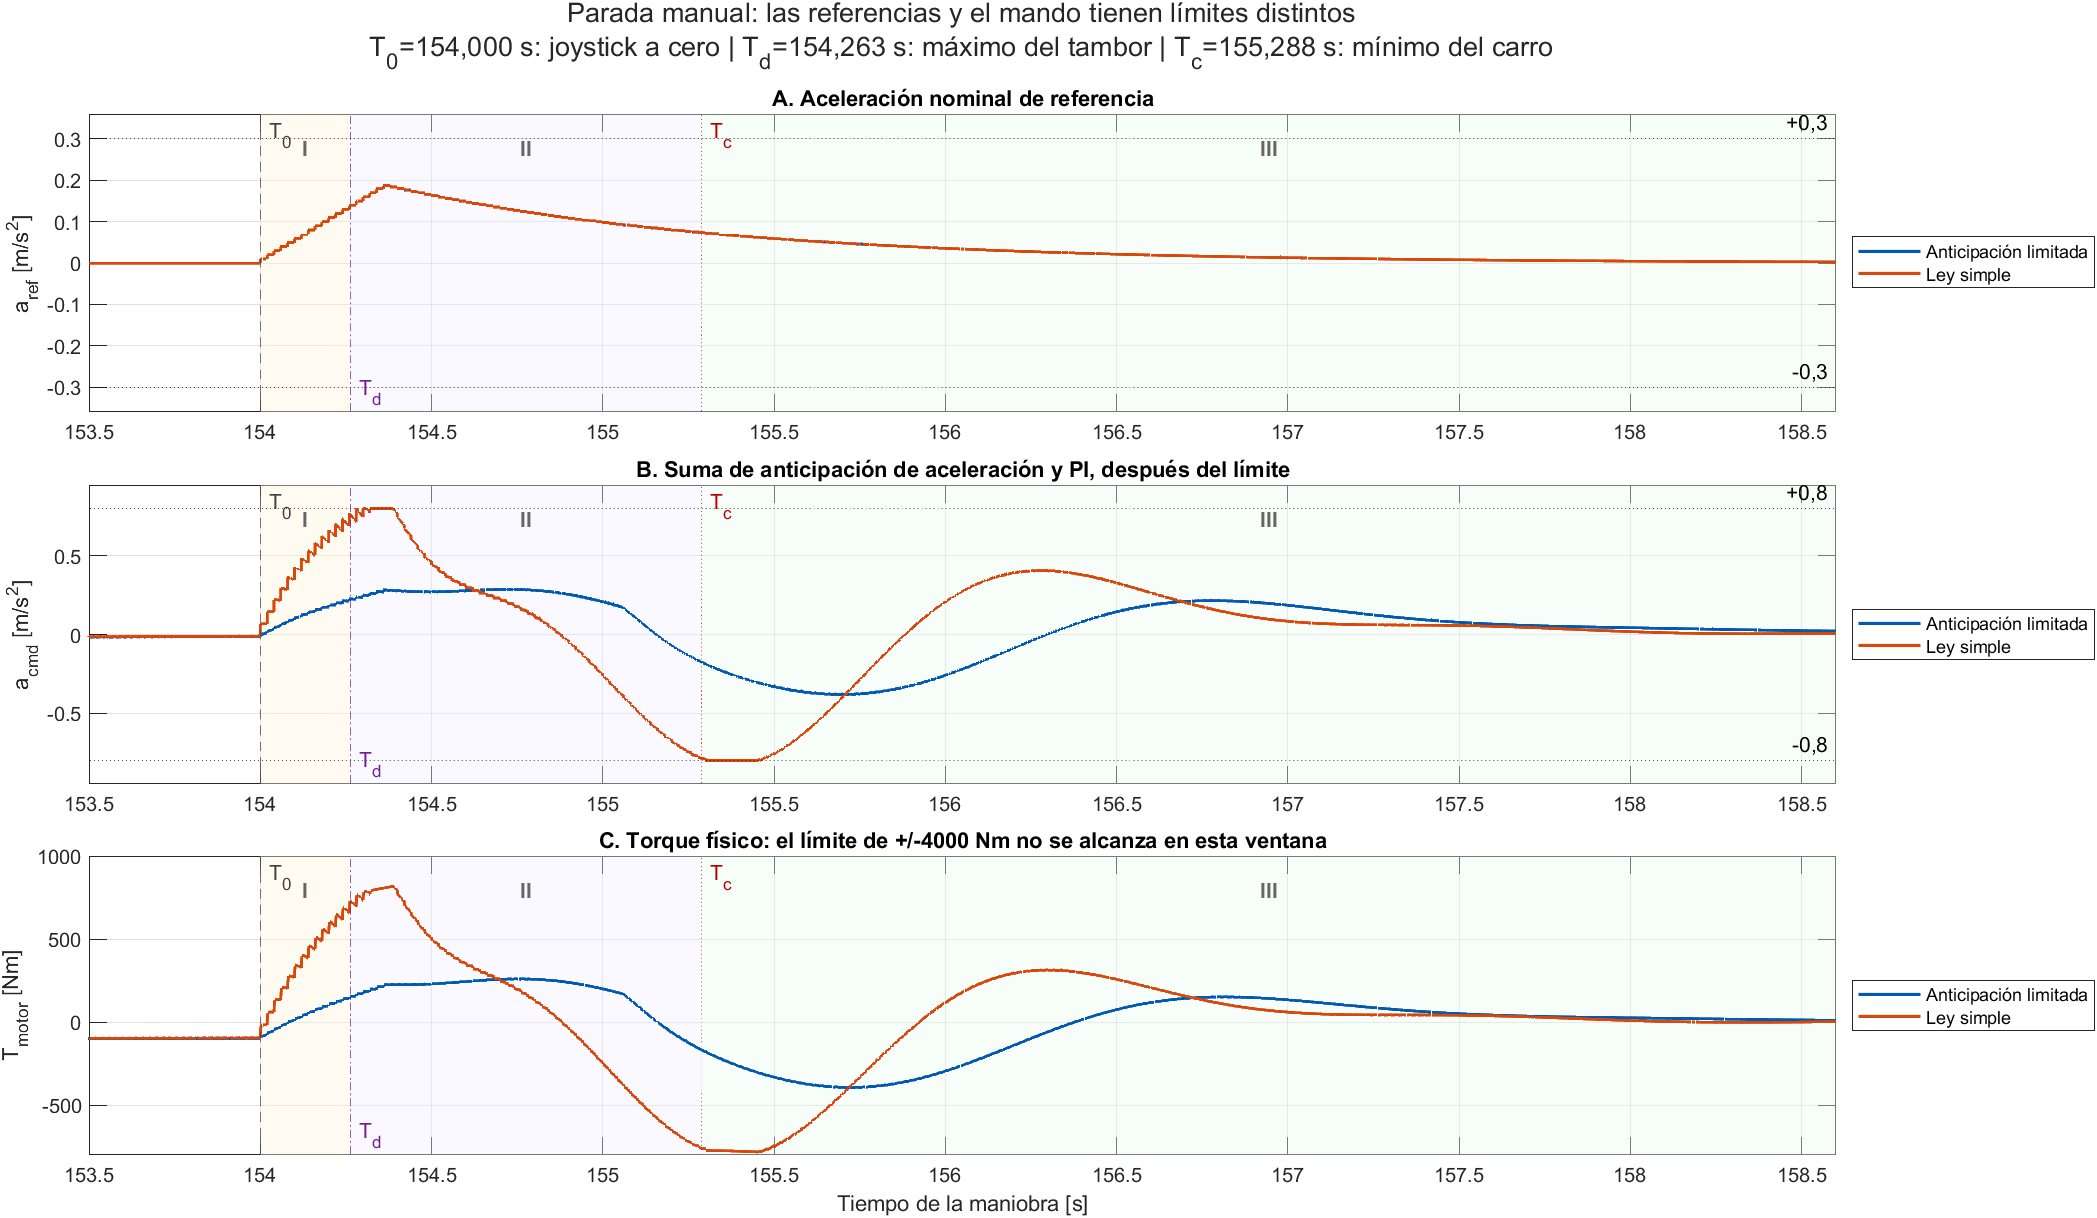
\includegraphics[width=0.99\textwidth,height=0.72\textheight,keepaspectratio]{imagenes_informe/usuario/integracionP1/03_02_referencias_y_mando.png}
\caption{A: aceleración nominal de referencia, con cotas \(\pm\)0,3 m/s\textsuperscript{2}. B: mando total después del límite \(\pm\)0,8 m/s\textsuperscript{2}. C: torque físico del motor, cuyo límite de \(\pm\)4000 Nm no se alcanza en esta ventana. Azul: anticipación anti-sway limitada. Naranja: ley simple. Las referencias temporales se definen a continuación y se mantienen en las \cref{fig:integracion_p1_3,fig:integracion_p1_4,fig:integracion_p1_5}.}
\label{fig:integracion_p1_3}
\end{figure}

\Needspace{5\baselineskip}

\subsubsection{Comprobación del esfuerzo y de la energía en la transmisión}

Para comprobar el origen mecánico del pico se analizaron la fuerza de transmisión, el desplazamiento relativo entre tambor y carro y la energía elástica almacenada, utilizando las relaciones del modelo de planta y de la sección~\ref{sec:integracion_p1}. La tabla y la figura siguientes comparan estas magnitudes durante la parada manual con ambas leyes antisway.

Las marcas $T_0$, $T_d$ y $T_c$ identifican la retirada del joystick a los $154{,}000~\mathrm{s}$, el máximo de aceleración del tambor a los $154{,}263~\mathrm{s}$ y el máximo negativo del carro a los $155{,}288~\mathrm{s}$, respectivamente, en la ley simple. Las zonas I, II y III abarcan los intervalos entre esas marcas y la respuesta posterior hasta $158{,}6~\mathrm{s}$.


\begin{table}[H]
\centering
{\small
\begin{tabular}{@{}L{0.42\textwidth}L{0.24\textwidth}L{0.26\textwidth}@{}}
\toprule
Magnitud en 154--158,6 s & Anticipación limitada & Ley simple\\
\midrule
Máximo absoluto de $a_t$ & 0,5641 m/s\textsuperscript{2} & 1,4535 m/s\textsuperscript{2}\\
Máximo absoluto de $a_{td}$ & 0,3678 m/s\textsuperscript{2} & 1,1602 m/s\textsuperscript{2}\\
Máxima fuerza absoluta $F_{tw}$ & 15,198 kN & 41,142 kN\\
Máxima deformación relativa absoluta $\lvert\delta\rvert$ & 31,655 mm & 85,686 mm\\
Máxima energía potencial elástica $U_{tw}$ & 240,485 J & 1762,084 J\\
Energía disipada por amortiguación en la ventana & 31,237 J & 264,157 J\\
Máximo torque motor absoluto & 394,611 Nm & 817,333 Nm\\
\bottomrule
\end{tabular}
}
\end{table}

\begin{figure}[H]
\centering
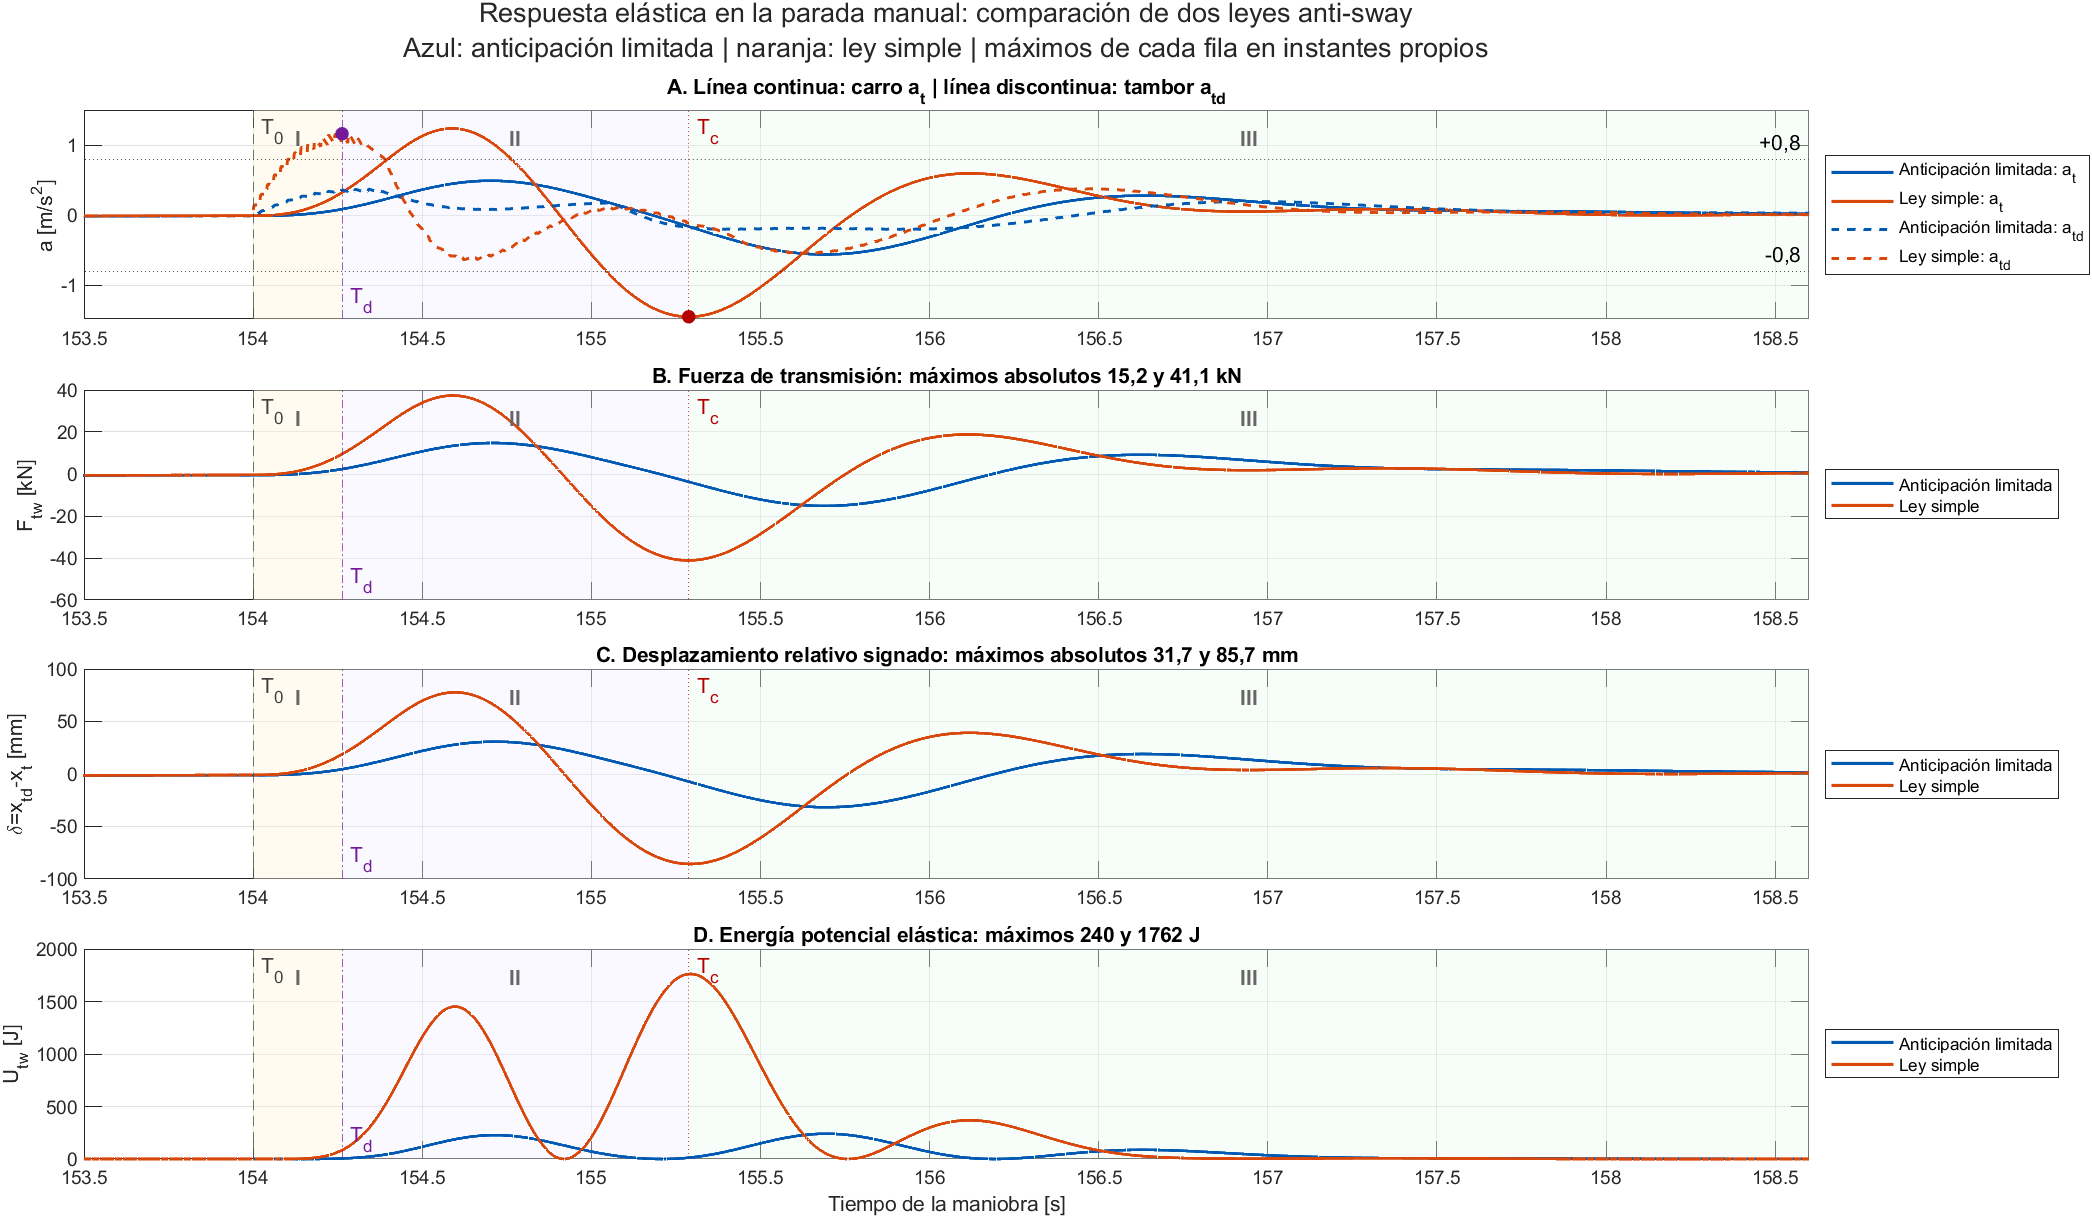
\includegraphics[width=0.99\textwidth,height=0.72\textheight,keepaspectratio]{imagenes_informe/usuario/integracionP1/04_03_fuerzas_deformacion_energia.png}
\caption{A: aceleraciones del carro, continuas, y del tambor, discontinuas. B: fuerza de transmisión. C: desplazamiento relativo signado. D: energía potencial elástica. Los colores azul y naranja conservan la identificación de las dos variantes en todos los paneles. Las marcas $T_0$, $T_d$ y $T_c$ corresponden a la ley simple; los fondos identifican las zonas I--III definidas en el texto. Las líneas horizontales \(\pm\)0,8 m/s\textsuperscript{2} son el criterio cinemático adoptado, no un límite admisible de esfuerzo mecánico.}
\label{fig:integracion_p1_4}
\end{figure}


Con la ley simple, el máximo del accionamiento precedió al pico del carro. En este último instante, la fuerza de transmisión fue aproximadamente $-41{,}14~\mathrm{kN}$, dominada por su componente elástica. El balance de fuerzas reproduce la aceleración de $-1{,}4535~\mathrm{m/s^2}$ y confirma la relación entre el pico y la deformación acumulada en la transmisión. El detalle concurrente se conserva en el anexo~\ref{anexo:balance_mecanico}.
\Needspace{5\baselineskip}

\subsubsection{Justificación de la modificación y elección de la variante}

Se selecciona la anticipación antisway limitada porque redujo aproximadamente un $63\%$ los máximos de fuerza y desplazamiento relativo y un $86{,}4\%$ la energía elástica máxima. La duración del ciclo varió solamente $0{,}198~\mathrm{s}$. La mejora corresponde a una menor excitación mecánica y al cumplimiento del criterio cinemático en la maniobra estudiada. El límite de pendiente de $0{,}25~\mathrm{m/s^2}$ conserva la acción directa de la realimentación angular y corresponde a una elección experimental para este ensayo.

Estos resultados no permiten establecer daño o resistencia mecánica admisible sin disponer de la geometría, pretensión y límites de esfuerzo de la transmisión.
\Needspace{5\baselineskip}

\subsection{Balance de la validación integrada}

La comparación integrada permitió evaluar la modificación de la anticipación antisway manteniendo los mismos límites, ganancias y antiwindup. Los resultados corresponden a las condiciones ensayadas; su ampliación requiere variar longitud, carga y sentido de parada. Para cuantificar el aporte del retrocálculo debe compararse una misma maniobra con y sin antiwindup.

La validación aislada de seguridad del apartado~\ref{sec:validacion_seguridad_stateflow} verifica la respuesta lógica, pero queda por evaluar su interacción con la planta durante una intervención: aplicación física de frenos, velocidad y distancia de parada, y recuperación con causas activas. Esta ampliación debe considerar las limitaciones de arranque, simultaneidad y rearme identificadas en el banco de pruebas.
\par
\Needspace{10\baselineskip}

\section{Implementación de los autómatas en CODESYS}
\label{sec:implementacion_codesys}
La etapa de implementación traslada al runtime CODESYS los autómatas supervisor y de seguridad. Se distinguen la traducción manual mediante SFC y ST auxiliar, la generación automática desde Stateflow y las adaptaciones de integración. Este apartado describe el software y su organización; los resultados de maniobras se presentan en la sección~\ref{sec:pruebas_SIL}.

\Needspace{5\baselineskip}

\subsection{Arquitectura de ejecución e intercambio de señales}
La planta y las mediciones permanecen en Simulink; OPC UA intercambia señales con CODESYS. El supervisor y la seguridad se ejecutan mediante programas y bloques de función del PLC. La configuración de tareas, el orden de llamadas y los permisos finales forman parte de la aplicación, además del núcleo de cada autómata. La implementación regulatoria como MC se presenta en la sección~\ref{sec:mc_p2}.

\Needspace{5\baselineskip}

\subsection{Implementación manual del supervisor}
\label{subsec:sup_manual_codesys}
\Needspace{5\baselineskip}
\subsubsection{Organización y ejecución de los programas}
El supervisor se distribuye en 16 programas SFC. Las salidas y los cálculos numéricos se implementan en ST: \path{PRG_PREPROCESO} acondiciona entradas y construye las banderas comunes, mientras \path{PRG_ACCIONES_Y_SALIDAS} consulta los pasos activos, calcula referencias y aplica interbloqueos finales. Las variables compartidas pertenecen a \path{GVL_GRUA}. Un paso activo se consulta mediante \texttt{Paso.x}; su permanencia se consulta mediante \texttt{Paso.t}. Los SFC exportados no contienen bloques de acción IEC: sus efectos se materializan en los programas ST de la tarea.

\path{MainTask_20ms} ejecuta una lista fija de llamadas cada $20~\mathrm{ms}$. Primero se procesa el enlace OPC UA y se ejecuta seguridad. Luego se ejecutan preprocesamiento, cuerda floja, contenedor paralelo, ciclo, modos, barrido, automático, carga, sobrecarga, fallas de carga, frenos y diagnóstico. El programa de acciones y salidas se llama al final. Por tanto, el orden entre POUs reemplaza parte del orden entre regiones paralelas de Stateflow; no debe suponerse que ambas organizaciones tienen idéntica semántica de ejecución.

\path{SFC_SUPERVISOR_PARALELO} contiene un paso inicial, una divergencia simultánea hacia cinco pasos de región y una convergencia hacia \texttt{DETENIDO}. Su retorno requiere reinicio y permiso global. Estos pasos expresan la organización concurrente; no invocan las secuencias subordinadas como acciones. Las secuencias se ejecutan porque la tarea las llama por separado. En los gráficos, el rectángulo doble identifica el paso inicial, la barra corta identifica una transición, la barra doble indica paralelismo y el salto identifica el destino de retorno.

\begin{figure}[!htb]
\centering
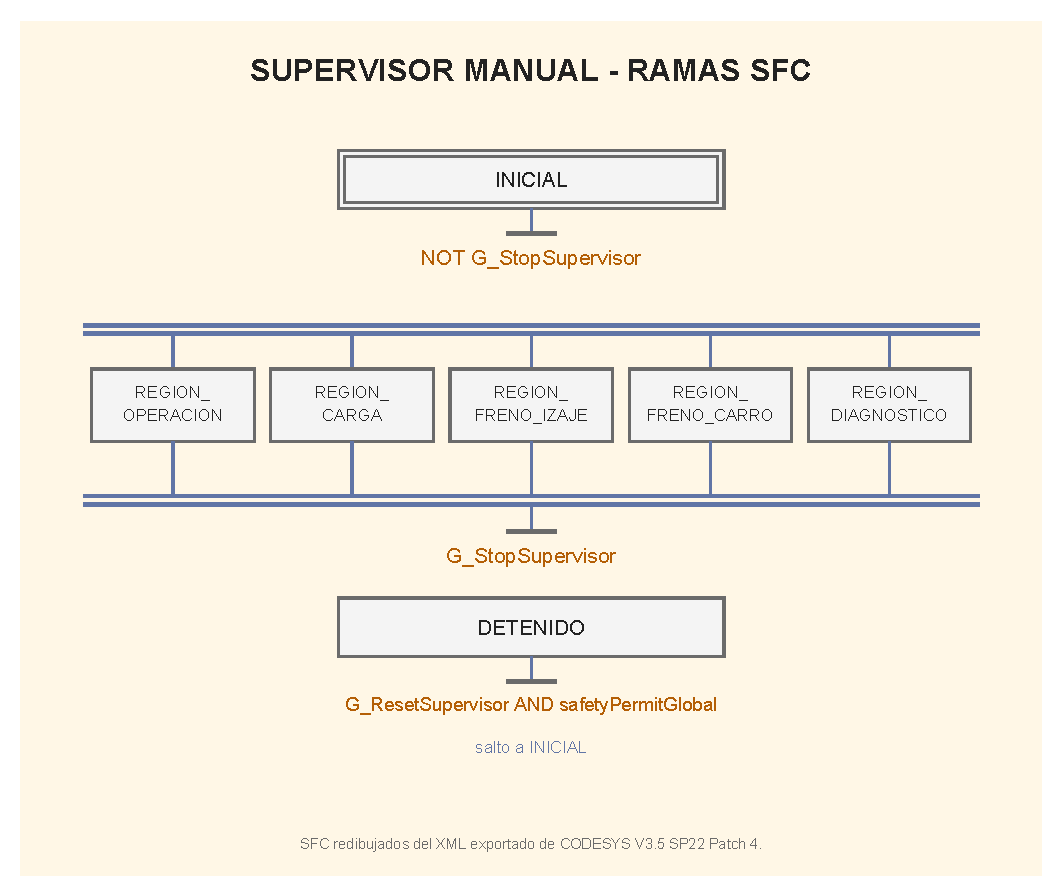
\includegraphics[width=0.96\textwidth]{imagenes_informe/otro/diagramas_codesys_manual/12_sfc_supervisor_paralelo.pdf}
\caption{SFC contenedor del supervisor manual. La divergencia y convergencia son simultáneas; la ejecución de los restantes POUs depende de la lista de llamadas de la tarea.}
\label{fig:sfc_supervisor_manual}
\end{figure}

\Needspace{5\baselineskip}

\subsubsection{Secuencias SFC de operación y transferencia de modo}
La región \texttt{OPERACION} de Stateflow se reparte entre tres SFC principales. \path{SFC_CICLO_SISTEMA} recorre \texttt{APAGADO}, \texttt{ARRANQUE}, \texttt{LISTO} y \texttt{PARADA\_NORMAL}. \texttt{LISTO} permanece activo durante las maniobras y funciona como habilitación de los SFC de modo; no equivale exclusivamente al código dos presentado por el HMI. El código efectivo se obtiene del arbitraje de salidas.

\path{SFC_MODO_MANUAL} contiene \texttt{MANUAL\_INACTIVO}, \texttt{MANUAL\_SUPERVISADO} y \path{APROXIMACION_FINAL_MANUAL}. La salida del manual supervisado hacia aproximación final ocurre por solicitud automática, solicitud de barrido o abandono del paso \texttt{LISTO}. Esta guarda difiere del Stateflow, donde la aproximación final se selecciona después del retorno desde un automático completado.

\path{SFC_MODO_AUTO} contiene espera, transferencia a automático, automático y transferencia a manual. Toda entrada recorre \path{BUMPLESS_A_AUTO}, con una permanencia mínima de $40~\mathrm{ms}$. Exige \texttt{LISTO} activo, solicitud e inicio automático, perfil válido, altura local suficiente, ausencia de sobrecarga y ausencia de intervención. No reproduce la entrada directa \texttt{LISTO} a \texttt{AUTOMATICO} del chart. El retorno a inactivo admite \texttt{allStopped}, que exige velocidades menores que $0.03~\mathrm{m/s}$ en ambos ejes, o la pérdida de \texttt{LISTO}.

\begin{figure}[!htb]
\centering
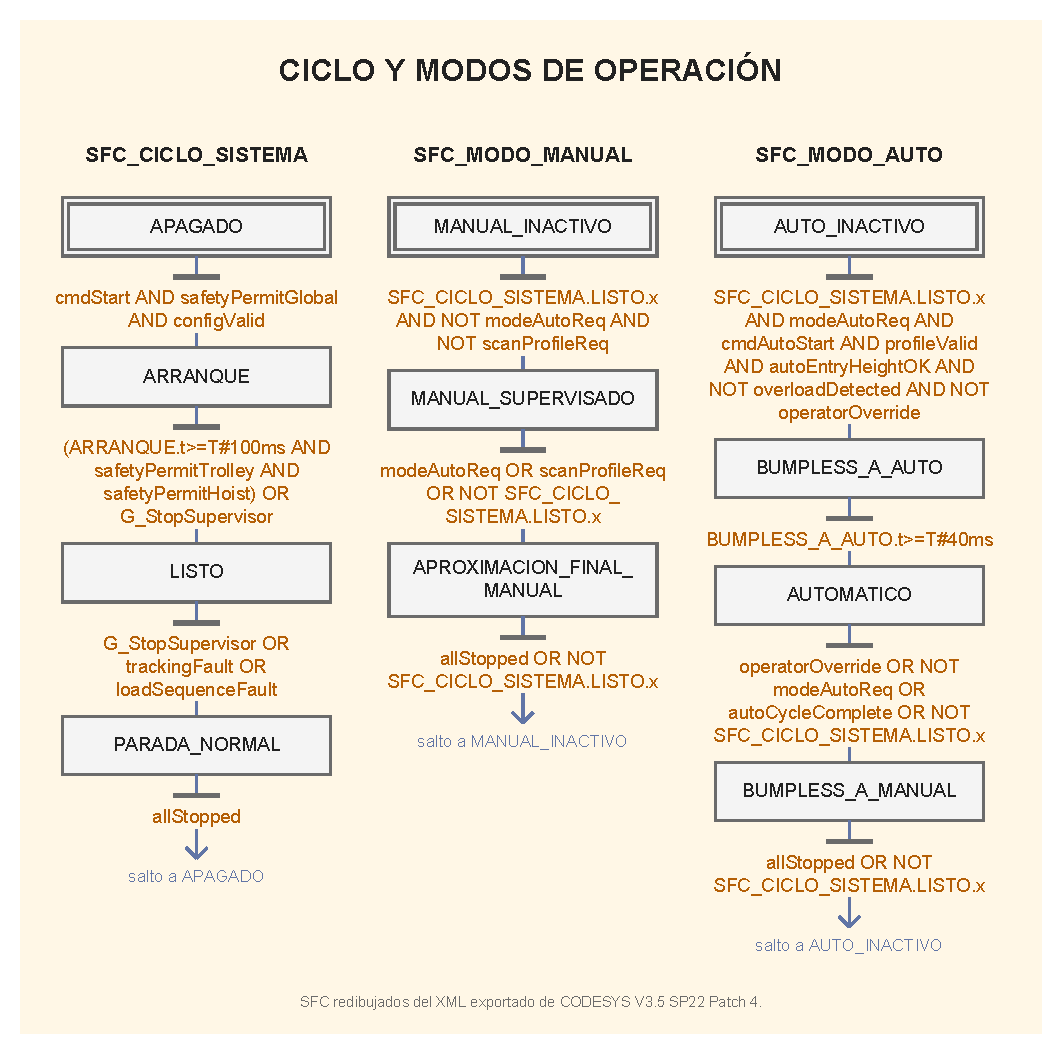
\includegraphics[width=0.98\textwidth,height=0.72\textheight,keepaspectratio]{imagenes_informe/otro/diagramas_codesys_manual/13_sfc_operacion.pdf}
\caption{SFC de ciclo, manual y automático. Las condiciones son las expresiones exportadas del proyecto, incluidas las referencias a pasos activos de otros POUs.}
\label{fig:sfc_modos_manual}
\end{figure}

\Needspace{5\baselineskip}

\subsubsection{SFC de barrido LiDAR y ejecución automática}
\path{SFC_ESCANEO_LIDAR} añade \texttt{ESPERA\_ESCANEO} a los cuatro pasos funcionales del relevamiento. Para comenzar exige \texttt{LISTO}, solicitud pendiente, perfil no completado, conjunto vacío y ejes detenidos. La preparación eleva hasta $39.65~\mathrm{m}$ con velocidad vertical pequeña. La condición derecha utiliza el límite normal o \texttt{lidarX}$\geq45.90~\mathrm{m}$ con velocidad pequeña; el Stateflow compara la posición del carro con $48.40~\mathrm{m}$. Se conserva el extremo izquierdo de $-24.50~\mathrm{m}$. La inicialización, registro y validación del perfil se efectúan en ST según el paso activo, incluida la precarga del \textit{slot} 33.

El XML del barrido es una cadena lineal: no contiene las transiciones laterales de parada o falla del chart. La pérdida de permisos se atiende mediante el ciclo principal y los interbloqueos de las salidas; no se dibujan rutas de escape inexistentes en este SFC.

\path{SFC_AUTOMATICO} recorre \texttt{ESPERA\_AUTO}, \texttt{PLANIFICAR}, \texttt{EJECUTAR} y \texttt{MANTENER\_OBJETIVO}. La planificación dura al menos $20~\mathrm{ms}$ y la llegada conserva los errores menores que $0.08~\mathrm{m}$ y $0.15~\mathrm{m}$. Las referencias se calculan en \path{PRG_ACCIONES_Y_SALIDAS}. Este proyecto utiliza el bloque \path{FB_craneTrajectoryQuintic}, con inicialización y evaluación explícitas, sin convertir los autómatas manuales en autómatas generados. La envolvente local, el objetivo seguro y la habilitación anti-sway siguen los criterios descritos para la referencia. La espera previa al descenso pertenece al planificador, no a una transición añadida al SFC.

\begin{figure}[!htb]
\centering
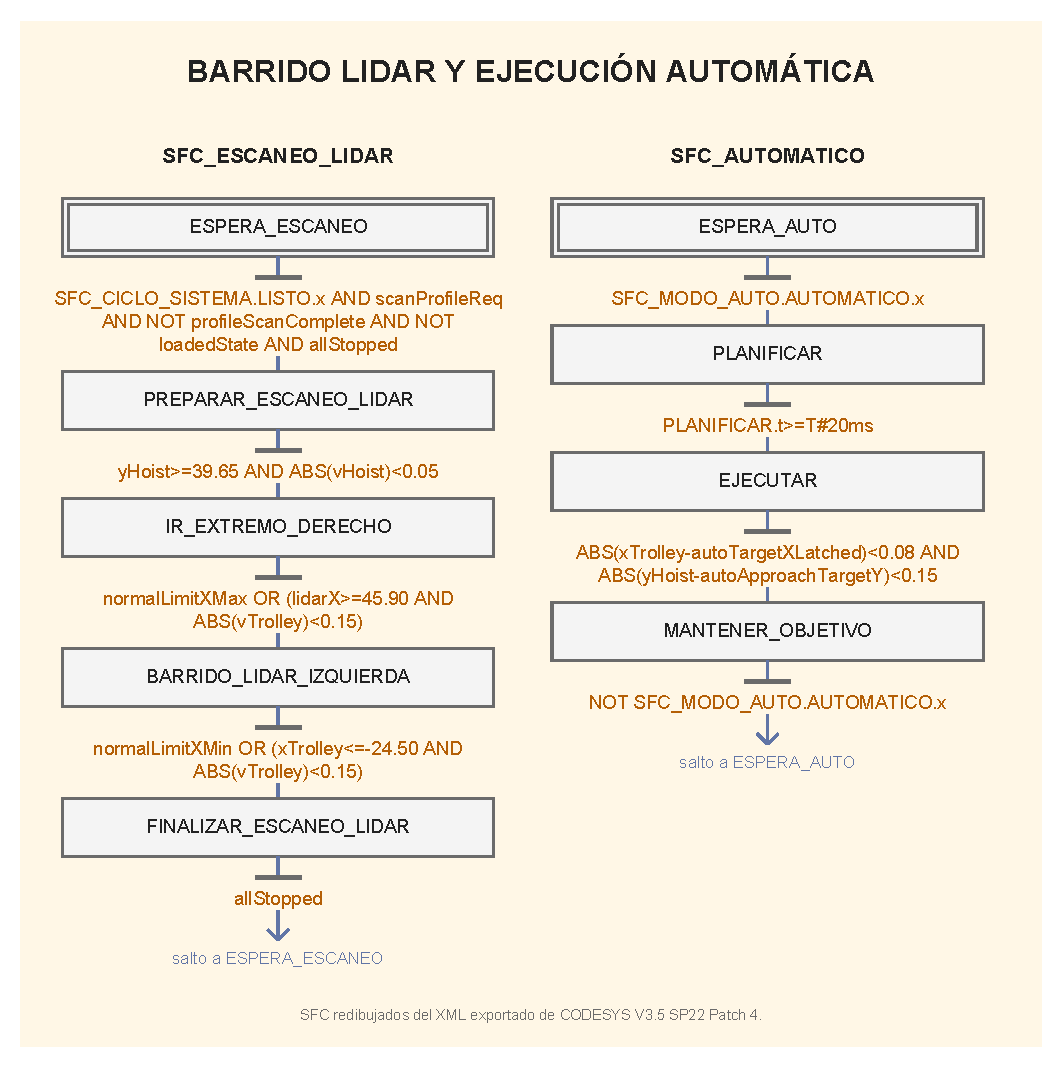
\includegraphics[width=0.98\textwidth,height=0.70\textheight,keepaspectratio]{imagenes_informe/otro/diagramas_codesys_manual/14_sfc_barrido_automatico.pdf}
\caption{SFC de relevamiento y automático interno de la versión manual de CODESYS. Las cadenas retornan por saltos a sus pasos iniciales.}
\label{fig:sfc_barrido_auto_manual}
\end{figure}

\Needspace{5\baselineskip}

\subsubsection{SFC de carga, pesaje y twistlocks}
La secuencia principal \path{SFC_CARGA} posee siete pasos: vacío, espera de estabilidad, cierre, despegue, pesaje, cargado y apertura. Conserva el contacto y permiso de izaje para iniciar el cierre, la estabilidad del spreader y las condiciones de cable tenso, velocidad y aceleración para iniciar el pesaje. En ST se acumula masa mientras \texttt{PESAJE.x} es verdadero; tras $500~\mathrm{ms}$ el SFC pasa a \texttt{CARGADO}.

Sobrecarga y falla de twistlocks se supervisan en POUs separados. \path{SFC_SOBRECARGA} detecta masa mayor que $50000~\mathrm{kg}$ con \texttt{CARGADO} activo. \path{SFC_FALLO_TWISTLOCK} detecta seguimiento fallido o permanencia de al menos $2~\mathrm{s}$ en cierre o apertura. Estas condiciones inhiben salidas mediante \texttt{loadSequenceFault}; no constituyen estados alternativos dentro de \path{SFC_CARGA}.

En Stateflow, el pesaje bifurca directamente hacia \texttt{CARGADO} o \texttt{SOBRECARGA}, y la espera de estabilidad puede cancelarse retornando a vacío. El SFC exportado no contiene esa cancelación ni la salida de despegue hacia apertura. Tampoco posee una transición de reinicio que reposicione por sí misma la cadena de carga al reconocer una falla. Estas diferencias explican por qué un reconocimiento del HMI no debe confundirse con un reinicio del estado interno de todos los SFC.

\begin{figure}[!htb]
\centering
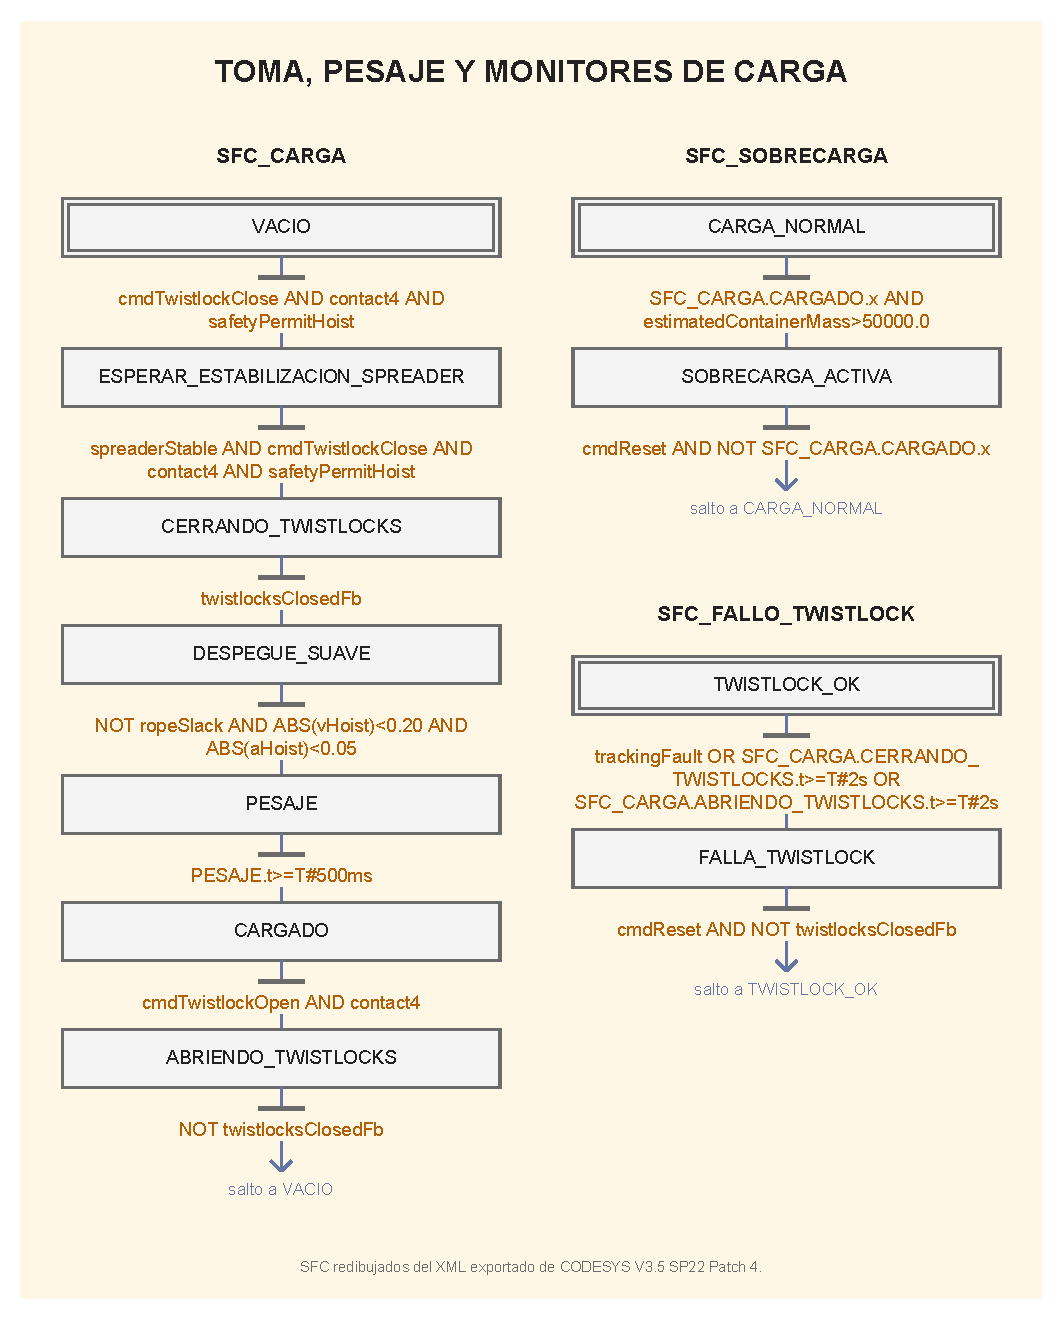
\includegraphics[width=0.98\textwidth,height=0.73\textheight,keepaspectratio]{imagenes_informe/otro/diagramas_codesys_manual/15_sfc_carga.pdf}
\caption{Cadena SFC de carga y monitores separados de sobrecarga y twistlocks. No se agregan bifurcaciones que solamente existen en el chart de Stateflow.}
\label{fig:sfc_carga_manual}
\end{figure}

\Needspace{5\baselineskip}

\subsubsection{SFC de frenos y comprobación de torque}
Los SFC de freno conservan los cuatro pasos aplicado, prueba de torque, abierto y aplicando. En izaje se conserva el criterio vertical de $0.05~\mathrm{m}$ y la excepción del modo automático ante ausencia momentánea de demanda. Sin embargo, el SFC de izaje no vuelve al paso aplicado por timeout de prueba; un monitor separado declara falla al superar $1~\mathrm{s}$ sin torque comprobado.

En carro se utiliza una tolerancia horizontal de $0.05~\mathrm{m}$, frente a $0.03~\mathrm{m}$ del chart. La transición desde prueba hacia abierto admite torque comprobado o cancelación de demanda, habilitación o permiso. El paso \texttt{TB\_ABIERTO} por sí solo no abre físicamente el freno: ST exige \texttt{brakeTrolleyProofLatched}, regulador habilitado, permisos y ausencia de falla de carga. La prueba queda memorizada para la maniobra vigente y se borra ante cancelación, pérdida de permiso o retorno a aplicado.



\begin{figure}[!htb]
\centering
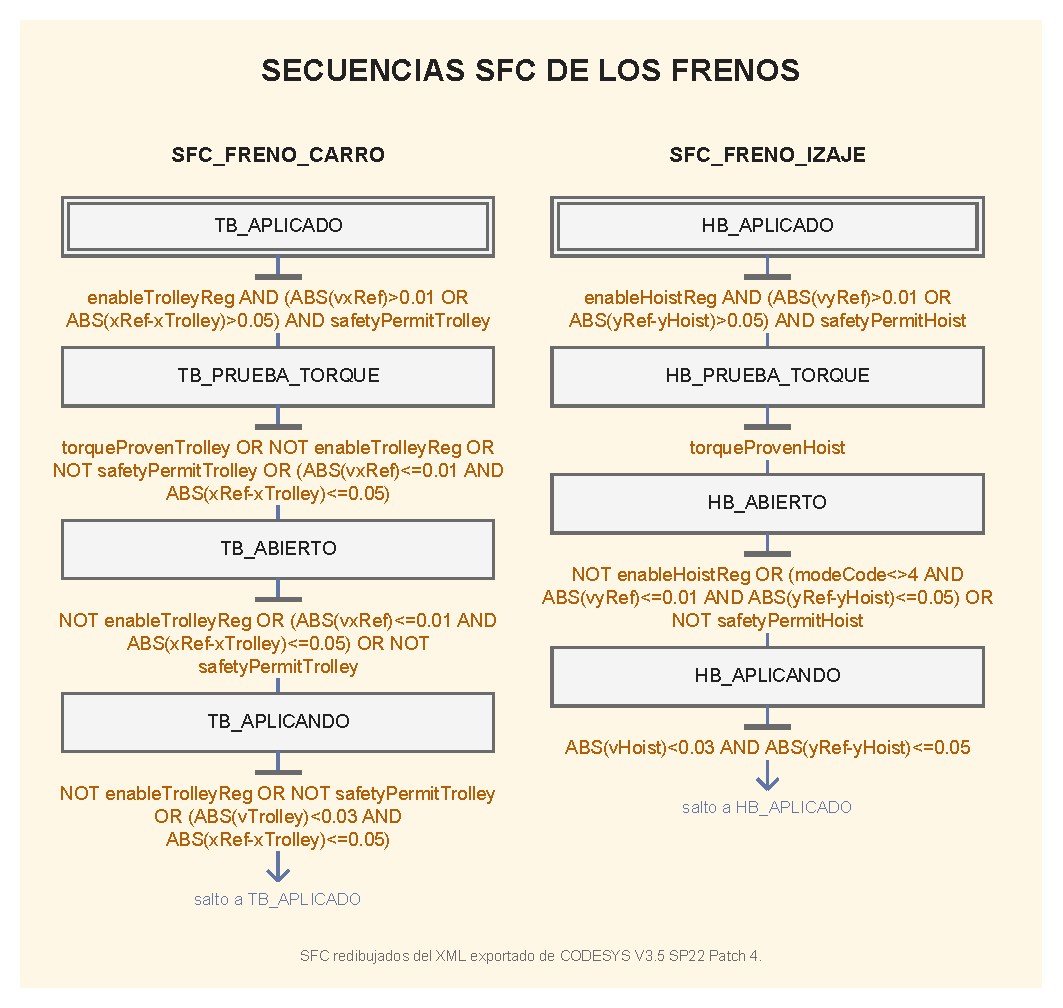
\includegraphics[width=0.98\textwidth,height=0.68\textheight,keepaspectratio]{imagenes_informe/otro/diagramas_codesys_manual/16_sfc_frenos.pdf}
\caption{Secuencias SFC de los frenos. Las autorizaciones físicas finales se calculan en ST y pueden ser más restrictivas que el paso activo.}
\label{fig:sfc_frenos_manual}
\end{figure}


El monitor de carro declara falla tras $8~\mathrm{s}$ de prueba sin torque, únicamente si persisten habilitación, permiso y demanda. Es una adaptación de la versión ensayada con el simulador, distinta del retorno por $50$ ticks del Stateflow. Los monitores de ambos frenos se incorporan a \texttt{loadSequenceFault}. Esta separación entre avance del SFC y salida física debe conservarse al interpretar los diagramas.

\begin{figure}[!htb]
\centering
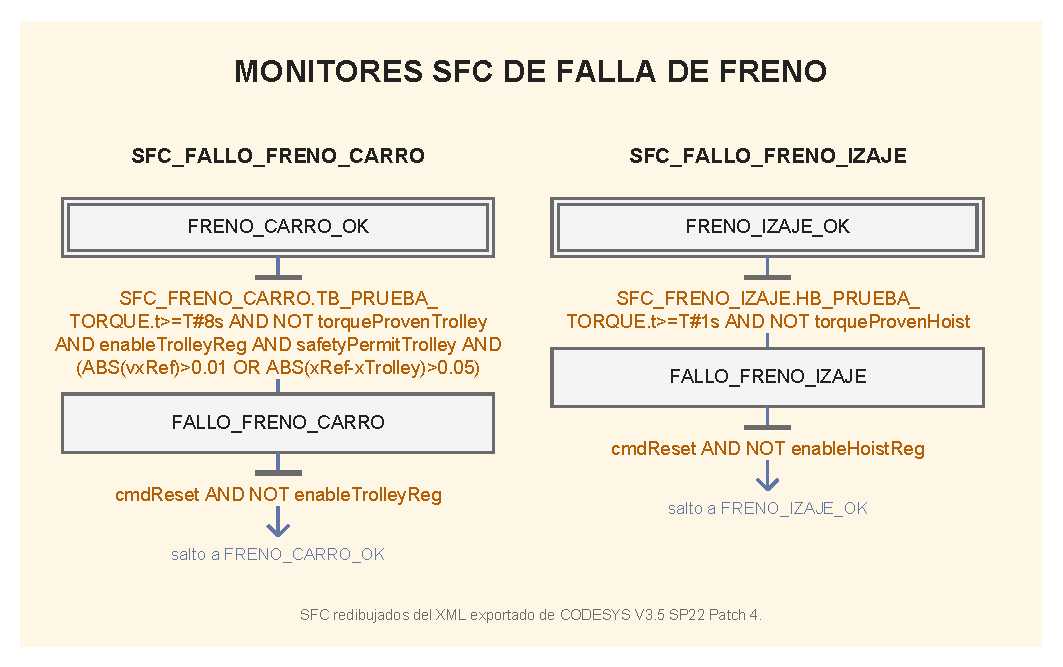
\includegraphics[width=0.98\textwidth]{imagenes_informe/otro/diagramas_codesys_manual/16b_sfc_fallas_frenos.pdf}
\caption{Monitores de falla de los frenos del carro y del izaje, con timeout y reconocimiento independientes.}
\label{fig:sfc_fallas_frenos_manual}
\end{figure}

\Needspace{5\baselineskip}

\subsubsection{SFC de cuerda floja y diagnóstico}
\path{SFC_CUERDA_FLOJA} materializa la histéresis de tensión mediante dos pasos: cambia a cuerda tensa por encima de $15000~\mathrm{N}$ y retorna a floja por debajo de $12000~\mathrm{N}$. En Stateflow esta memoria se implementa en una función auxiliar.

\path{SFC_ALARMA_SOBRECARGA} y \path{SFC_FALLO_SUPERVISOR} son monitores de dos pasos. El primero reconoce la alarma con reinicio y desaparición de sobrecarga; el segundo retiene seguimiento fallido, falla de carga o ausencia de permiso global. Los códigos se calculan en preprocesamiento y se publican en el arbitraje final. Como varios pasos pueden estar activos simultáneamente, la prioridad efectiva depende de las ramas \texttt{IF/ELSIF} del programa ST, además del orden de llamadas. No corresponde atribuirles el único estado exclusivo \texttt{DIAG\_OK/ALARMA/FALLA} del chart.

\begin{figure}[!htb]
\centering
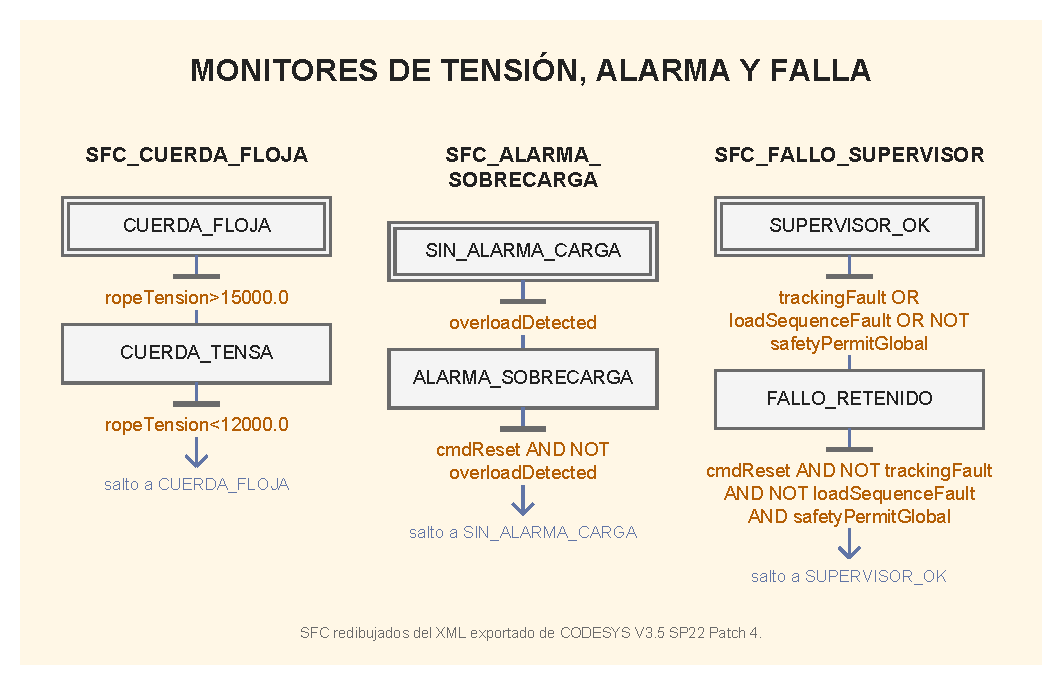
\includegraphics[width=0.98\textwidth]{imagenes_informe/otro/diagramas_codesys_manual/17_sfc_diagnostico.pdf}
\caption{SFC auxiliares de tensión, alarma por sobrecarga y falla retenida del supervisor manual.}
\label{fig:sfc_diag_manual}
\end{figure}

\Needspace{5\baselineskip}

\subsubsection{Comparación del supervisor: Stateflow y CODESYS manual}
Ambas implementaciones comparten las señales físicas, los objetivos locales, la toma estable, la generación de referencias y los permisos de seguridad. La traducción manual distribuye la secuencia y sus acciones entre POUs; conserva el objetivo funcional, pero no constituye una equivalencia completa del grafo jerárquico ni de sus prioridades.

{\footnotesize
\Needspace{12\baselineskip}
\begin{longtable}{L{3.0cm} L{5.8cm} L{5.8cm}}
\caption{Correspondencias y diferencias verificadas del supervisor.}\label{tab:comparacion_sup_sfc}\\
\toprule
Aspecto & Stateflow de referencia & CODESYS manual SFC\\
\midrule
\endfirsthead
\toprule Aspecto & Stateflow de referencia & CODESYS manual SFC\\\midrule
\endhead
Organización & Cinco regiones paralelas dentro de un chart; frenos con dos subregiones. & Dieciséis programas SFC y programas ST de preprocesamiento/salidas llamados por una tarea.\\
Acciones & Entrada, ejecución y salida de estados; funciones MATLAB del chart. & Estados consultados mediante \texttt{Paso.x}; acciones en ST, sin bloques de acción en los SFC exportados.\\
Estado listo & Estado de operación previo a seleccionar manual o automático. & Paso del ciclo que permanece activo y habilita secuencias de modo independientes.\\
Entrada automática & Directa desde LISTO; desde manual utiliza dos ticks de transferencia. & Siempre utiliza BUMPLESS\_A\_AUTO con al menos 40 ms; añade ausencia de intervención desde LISTO.\\
Guarda automática & Desde manual exige ciclo no completo; altura local y perfil válido en ambas entradas. & Conserva perfil y altura local; la guarda de entrada no comprueba \texttt{autoCycleComplete}.\\
Salida automática & Bumpless hacia manual por objetivo, intervención o cancelación. & Añade pérdida de LISTO; retorno por \texttt{allStopped} o pérdida de LISTO.\\
Aproximación manual & Posterior al automático completado; sale al liberar carga. & Paso del SFC manual alcanzado por solicitud auto/barrido o pérdida de LISTO; sale por reposo o pérdida de LISTO.\\
Barrido & Estados con salidas laterales de parada/falla; extremo derecho en \texttt{xTrolley}. & Cadena sin escapes laterales; extremo derecho en \texttt{lidarX}; inhibición final de salidas en ST.\\
Carga y sobrecarga & Bifurcación de pesaje a cargado/sobrecarga; falla y cancelación dentro de la región. & Pesaje de 500 ms a cargado; sobrecarga y falla en monitores separados.\\
Freno del carro & Prueba de torque con retorno por 50 ticks; tolerancia de posición 0.03 m. & Monitor de 8 s; tolerancia de 0.05 m; prueba memorizada necesaria para apertura física.\\
Freno de izaje & Retorno al aplicado por timeout de 50 ticks. & Monitor separado de 1 s sin transición de timeout en la secuencia del freno.\\
Diagnóstico & Máquina exclusiva OK/alarma/falla. & Monitores concurrentes y arbitraje de códigos en ST.\\
Tiempo & Ticks y segundos del motor de simulación de Stateflow. & Permanencia \texttt{Paso.t} y acumuladores en la tarea PLC de 20 ms; tiempo de pared.\\
\bottomrule
\end{longtable}}

Los diagramas SFC permiten inspeccionar la secuencia real y la tabla permite localizar los cambios de estructura. La comparación no demuestra equivalencia temporal de todos los eventos concurrentes; en las pruebas OPC UA, Simulink y el PLC no están sincronizados por pasos. El planificador quíntico generado dentro del proyecto manual no cambia el lenguaje SFC de estos autómatas.

\Needspace{5\baselineskip}

\subsection{Implementación manual de seguridad}
\label{subsec:seg_manual_codesys}
\Needspace{5\baselineskip}
\subsubsection{Organización del nivel de seguridad}
La versión manual distribuye protección en cinco SFC: un contenedor paralelo y cuatro monitores de carro, izaje, watchdog y emergencia total. \path{PRG_PRESEGURIDAD} calcula los flancos y la temporización; \path{PRG_SALIDAS_SEGURIDAD} arbitra las autorizaciones y permisos. Estos programas se ejecutan antes del supervisor en \path{MainTask_20ms}.

La secuencia exacta es: enlace OPC UA, preseguridad, SFC de carro, SFC de izaje, SFC de watchdog, SFC total, contenedor paralelo y salidas de seguridad. Los cuatro monitores se llaman en cada ciclo, independientemente de las acciones del contenedor. \path{SFC_AUTOMATA_SEGURIDAD} mantiene sus dos pasos de región porque la transición posterior a la convergencia tiene condición \texttt{FALSE}; su representación expresa paralelismo, pero no selecciona por sí misma las salidas de emergencia.

\begin{figure}[!htb]
\centering
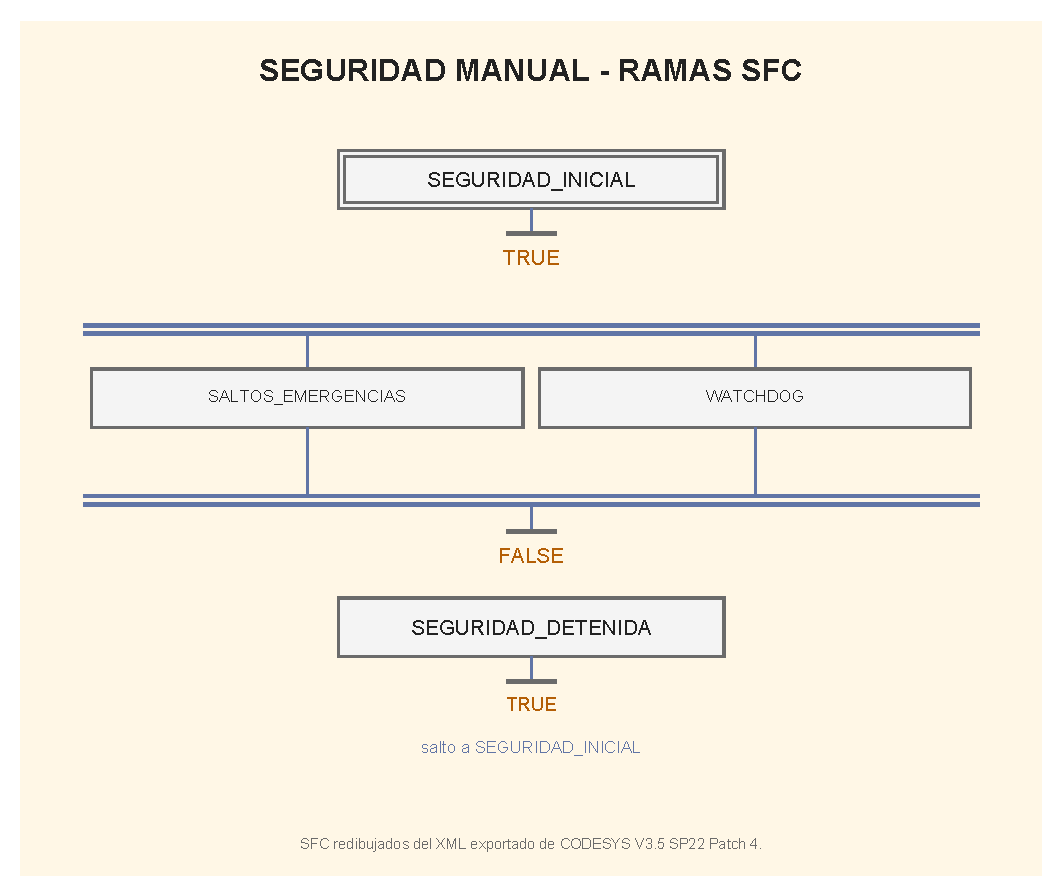
\includegraphics[width=0.96\textwidth]{imagenes_informe/otro/diagramas_codesys_manual/18_sfc_seguridad_paralela.pdf}
\caption{Contenedor SFC paralelo del nivel de seguridad manual. Los SFC de detección y el arbitraje de salidas se ejecutan mediante llamadas separadas de la tarea.}
\label{fig:sfc_seg_paralela}
\end{figure}

\Needspace{5\baselineskip}

\subsubsection{SFC de emergencias parciales por eje}
\path{SFC_SEG_CARRO} posee los pasos \texttt{CARRO\_SEGURO} y \texttt{EMERGENCIA\_CARRO}; \path{SFC_SEG_IZAJE} posee \texttt{IZAJE\_SEGURO} y \texttt{EMERGENCIA\_IZAJE}. Los flancos de límites últimos y sobrevelocidad proceden del preprocesamiento. El rearme de cada monitor exige flanco de reinicio y desaparición de los sensores de su propio eje.

Los monitores pueden quedar activos simultáneamente. Así se reconocen los flancos de ambos ejes en la misma llamada de tarea, y el monitor total y el arbitraje pueden producir inhibición total. Esta organización difiere de las transiciones alternativas ordenadas desde el único estado normal de Stateflow. Los monitores parciales no comprueban el pulsador de emergencia en su guarda de recuperación; su efecto se conserva mediante el monitor total y el arbitraje final.

\begin{figure}[!htb]
\centering
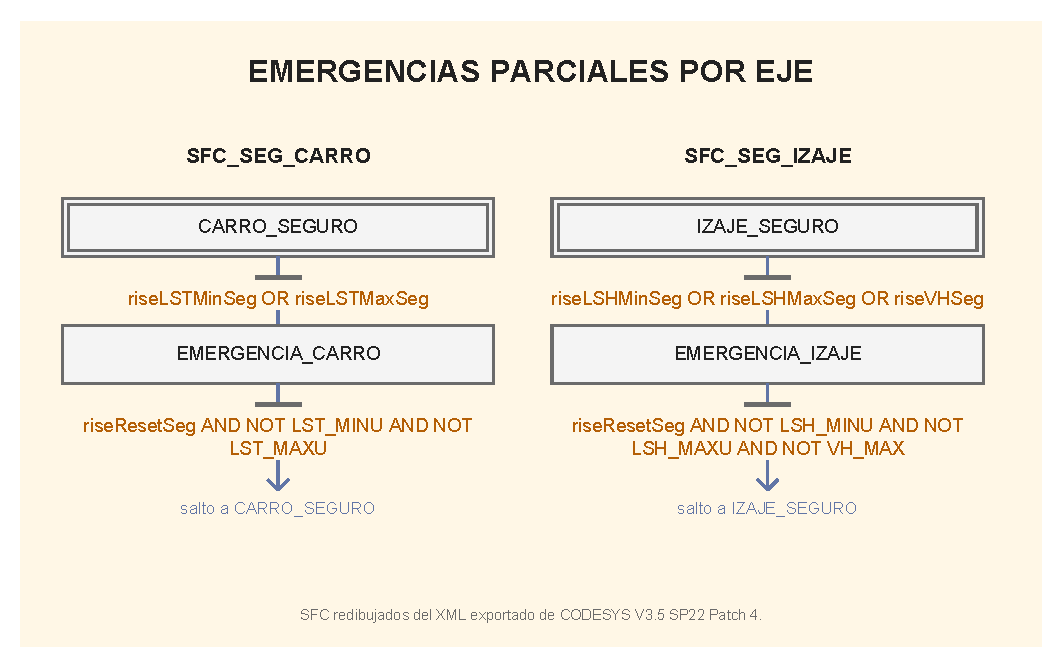
\includegraphics[width=0.98\textwidth]{imagenes_informe/otro/diagramas_codesys_manual/19_sfc_seguridad_ejes.pdf}
\caption{Monitores SFC independientes de emergencia del carro y del izaje, con sus condiciones exactas de disparo y rearme.}
\label{fig:sfc_seg_ejes}
\end{figure}

\Needspace{5\baselineskip}

\subsubsection{SFC de watchdog y emergencia total}
El preprocesador compara \texttt{pulso\_WD} con su valor anterior. Ante cambio pone a cero el acumulador; de lo contrario suma $0.02~\mathrm{s}$. \path{SFC_SEG_WATCHDOG} pasa a disparado cuando el acumulador alcanza $\max(0.02,\allowbreak\texttt{TiempoMaxWD})$. Su retorno exige reinicio y desaparición del timeout. En el archivo del proyecto, el valor inicial de \texttt{TiempoMaxWD} es $5~\mathrm{s}$. El watchdog de la tarea, configurado a $100~\mathrm{ms}$, es un mecanismo diferente y no debe confundirse con esta vigilancia del pulso.

\path{SFC_SEG_TOTAL} detecta pulsador, falla OPC UA, watchdog disparado o coexistencia de emergencias de ambos ejes. Su recuperación exige reinicio y ausencia de todas esas condiciones. El watchdog se ejecuta antes del SFC total, por lo que su nuevo paso puede ser consumido por el monitor total dentro de la misma llamada de tarea. También pueden limpiarse los monitores antes de evaluar el rearme total si todas sus guardas son verdaderas; no se traslada automáticamente a esta implementación la particularidad de dos flancos del chart.

La falla de comunicación se obtiene en \path{PRG_ENLACE_OPCUA} por ausencia de cambios del latido de Simulink. \texttt{opcTimeoutSeconds} se inicializa a $1~\mathrm{s}$ en el proyecto; puede configurarse para el ensayo. Estos valores describen el archivo exportado, no una lectura de parámetros activos del runtime. La vigilancia de comunicación es una protección adicional necesaria para esta arquitectura repartida entre PLC y Simulink.

\begin{figure}[!htb]
\centering
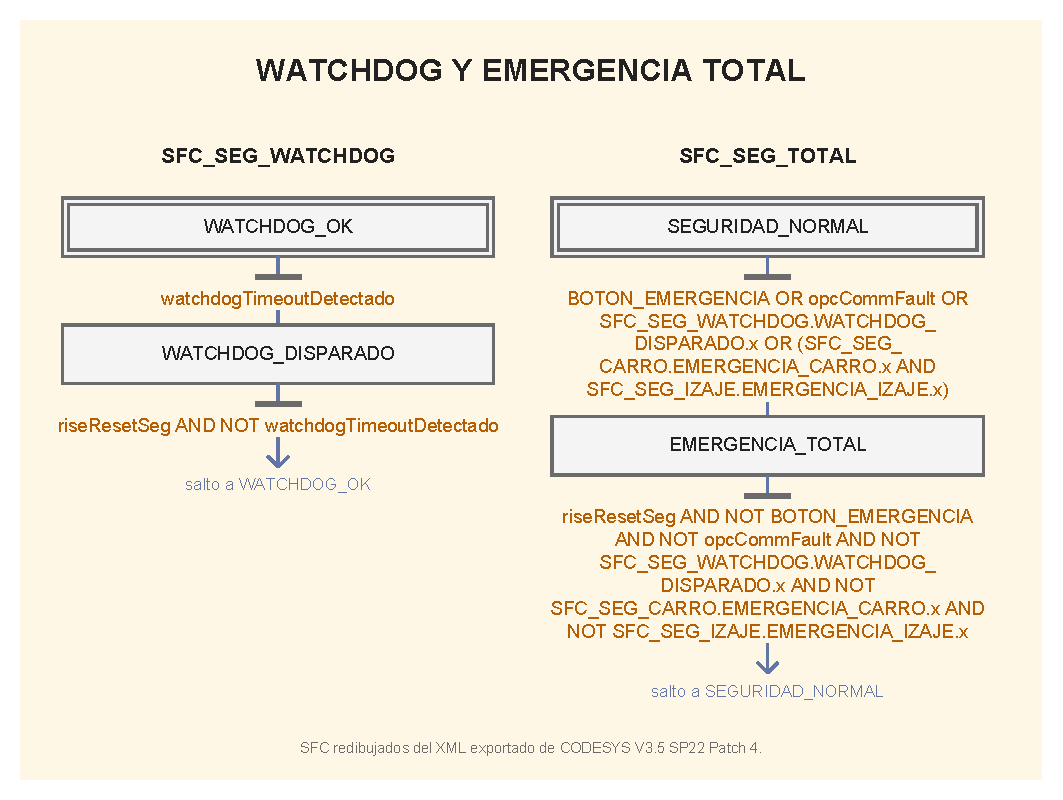
\includegraphics[width=0.98\textwidth]{imagenes_informe/otro/diagramas_codesys_manual/20_sfc_watchdog_total.pdf}
\caption{SFC de watchdog y emergencia total. La comunicación OPC UA interviene explícitamente en disparo y recuperación.}
\label{fig:sfc_wd_total}
\end{figure}

\Needspace{5\baselineskip}

\subsubsection{Comparación de seguridad: Stateflow y CODESYS manual}
El arbitraje ST utiliza prioridad total, coincidencia de parciales, izaje, carro y normal. Mantiene la polaridad activa en uno de \texttt{BRK\_t}, \texttt{BRK\_h} y \texttt{BRK\_hE}, pero transforma sus permisos de manera diferente al subsistema Stateflow:
\begin{align}
\texttt{safetyPermitGlobal}&=\neg\texttt{EMERGENCIA}\notag\\
&\quad\land\neg\texttt{PARADA\_EMERGENCIA\_WD}\land\neg\texttt{opcCommFault},\\
\texttt{safetyPermitTrolley}&=\texttt{safetyPermitGlobal}\land\texttt{BRK\_t},\\
\texttt{safetyPermitHoist}&=\texttt{safetyPermitGlobal}\land\texttt{BRK\_h}\land\texttt{BRK\_hE}.
\end{align}
En consecuencia, una emergencia parcial anula el permiso global y ambos permisos de movimiento en CODESYS manual, aun cuando la autorización de freno del eje no afectado permanezca verdadera. El programa final del supervisor fuerza además las órdenes de apertura a falso cuando falta el permiso global. No corresponde aplicar a esta versión la matriz del Stateflow, cuyo permiso global se calcula con OR de las autorizaciones de eje.

\begin{table}[!htb]
\centering\small
\caption{Permisos efectivos: diferencia ante emergencias parciales.}\label{tab:permisos_sfc_vs_sf}
\begin{tabular}{L{4.0cm} C{1.3cm} C{1.3cm} C{1.3cm} C{1.3cm} C{1.3cm} C{1.3cm}}
\toprule
& \multicolumn{3}{c}{Stateflow} & \multicolumn{3}{c}{CODESYS manual}\\
Condición & Global & Carro & Izaje & Global & Carro & Izaje\\
\midrule
Normal & 1 & 1 & 1 & 1 & 1 & 1\\
Emergencia de carro & 1 & 0 & 1 & 0 & 0 & 0\\
Emergencia de izaje & 1 & 1 & 0 & 0 & 0 & 0\\
Emergencia total & 0 & 0 & 0 & 0 & 0 & 0\\
\bottomrule
\end{tabular}
\end{table}

{\footnotesize
\Needspace{12\baselineskip}
\begin{longtable}{L{3.0cm} L{5.8cm} L{5.8cm}}
\caption{Diferencias de estructura y ejecución del nivel de seguridad.}\label{tab:comparacion_seg_sfc}\\
\toprule Aspecto & Stateflow de referencia & CODESYS manual SFC\\\midrule
\endfirsthead
\toprule Aspecto & Stateflow de referencia & CODESYS manual SFC\\\midrule
\endhead
Estados & Región de emergencia con cuatro estados exclusivos y watchdog con dos estados. & Cuatro monitores independientes de dos pasos y un contenedor paralelo.\\
Simultaneidad de ejes & Prioridad de transición: total, izaje, carro; puede consumir sólo uno de los flancos desde normal. & Ambos monitores reconocen sus flancos en la misma tarea; la coincidencia genera total.\\
Emergencia parcial & Mantiene permiso global y el eje no afectado autorizado. & Anula permiso global y ambos movimientos.\\
Pérdida de comunicación & No integra una entrada OPC UA al chart de referencia. & \texttt{opcCommFault} provoca total y mantiene permisos inhibidos.\\
Watchdog & Emergencias antes de watchdog; reconocimiento de su solicitud en activación siguiente. & Watchdog antes de total y salidas; consumo del nuevo paso dentro de la tarea.\\
Rearme watchdog & Flanco de reinicio como guarda de salida del fallo. & Flanco de reinicio y timeout inactivo.\\
Cambio en el vencimiento & Transición por vencimiento se evalúa antes de realimentar por cambio. & Preprocesador reinicia el acumulador ante cambio antes de evaluar timeout.\\
Acciones de protección & Asignadas en la entrada de cada estado del chart. & Calculadas cada llamada en ST a partir de pasos activos y comunicación.\\
\bottomrule
\end{longtable}}

La comparación se fundamenta en el XML y los programas ST exportados. Describe las diferencias de arquitectura y comportamiento encontradas en el simulador; no se presupone equivalencia completa con el chart.

\Needspace{5\baselineskip}

\subsection{Generación automática del supervisor e integración}
\label{subsec:sup_generado_codesys}
\Needspace{5\baselineskip}
\subsubsection{Generación y estructura del código}
La implementación automática del supervisor y del autómata de seguridad se realizó mediante la generación automática de código para PLC de Simulink, utilizando Simulink PLC Coder con destino CODESYS.

La generación produce XML de intercambio con cuerpos en Structured Text. No produce diagramas SFC nuevos: la representación gráfica de referencia sigue siendo el chart de Stateflow de las Figuras anteriores. El bloque principal \path{FB_GEN_SUPERVISOR} representa la jerarquía mediante variables de estado, constantes, estructuras \texttt{CASE}, condiciones y funciones auxiliares. Los comentarios del ST conservan referencias a elementos del modelo. Las acciones de entrada, ejecución y salida quedan integradas en ese código, en lugar de repartirse entre pasos SFC y programas de acciones escritos manualmente.

La salida original contiene 27 POUs del supervisor y 3 de protección. Estos recuentos incluyen bloques auxiliares y no son números de estados. La integración utiliza tres llamadas en \path{MainTask_20ms}, en este orden: \path{PRG_ENLACE_OPCUA}, \path{PRG_AUTO_SEGURIDAD} y \path{PRG_AUTO_SUPERVISOR}. La tarea tiene intervalo de 20 ms, prioridad 1 y watchdog de 100 ms. En la copia automática final se retiraron los 21 SFC manuales. Tener el ST generado importado junto a los SFC antiguos no basta para identificar qué implementación está activa: debe verificarse también la lista de llamadas de la tarea.

Los adaptadores inicializan cada instancia una vez con \texttt{SS\_INITIALIZE} y luego ejecutan \texttt{SS\_STEP} en cada llamada. La planta, los reguladores, los sensores, el HMI y la visualización permanecen en Simulink. OPC UA intercambia medidas y órdenes mediante \path{GVL_GRUA}; el adaptador no traslada al PLC la dinámica de la grúa.

\Needspace{5\baselineskip}

\subsubsection{Adaptaciones de importación e interfaz}
El adaptador conecta 33 entradas y 39 salidas del supervisor. Cuatro entradas cambian de nombre al conectarse con la interfaz existente: \texttt{omega\_td\_est} recibe \texttt{omegaTrolley}, \texttt{y\_l} recibe \texttt{yHoist}, \texttt{v\_ly} recibe \texttt{vHoist} y \texttt{F\_hw\_sens} recibe \texttt{ropeTension}. Convierte \texttt{modeCode} de \texttt{LREAL} a \texttt{INT} y copia los perfiles de índices $[0..32]$ del bloque generado a los índices $[1..33]$ de OPC UA. Un desplazamiento incorrecto de índices cambiaría la correspondencia física de los slots.

Después del STEP se aplican compuertas de permisos a habilitaciones y órdenes de apertura de frenos. Si se ordena cerrar twistlocks se fuerza a falso su orden de apertura. Estas operaciones pertenecen a la integración escrita para CODESYS; no deben atribuirse a una transformación automática del chart. Asimismo, el temporizador generado para protección requiere el tipo calificado \texttt{Standard.TON} en esta instalación y la biblioteca Standard utilizada por el proyecto.

\Needspace{5\baselineskip}

\subsubsection{Diferencia temporal detectada en la generación}
El principal problema encontrado al ejecutar la primera versión no fue una guarda de transición distinta, sino una incompatibilidad entre la base temporal del código exportado y la tarea que lo llamaba. La cabecera del XML original declara una muestra de subsistema de $1~\mathrm{ms}$. PLC Coder insertó contadores con divisores 20 y 40 para atender tasas de 20 y 40 ms del modelo. Esos divisores sólo mantienen las tasas esperadas si la llamada externa conserva la base de 1 ms.

La tarea CODESYS llamaba al bloque cada 20 ms. Por ello, el primer divisor activaba la lógica del supervisor cada $20\times20=400~\mathrm{ms}$; la segunda tasa pasaba a $40\times20=800~\mathrm{ms}$. Los pulsos del HMI de 40 ms podían quedar completos entre dos ejecuciones de la lógica. En el intento registrado, la comunicación cifrada funcionó, pero el modo permaneció en cero durante 186.72 s de simulación después de START y no comenzó el barrido. Una nueva pulsación tampoco inició la secuencia.

La corrección se aplicó al ST preparado para importación: los umbrales de los contadores se cambiaron de 19 y 39 a 0 y 1, respectivamente. Así, con la tarea de 20 ms, el primer grupo se atiende en cada llamada y el segundo cada dos llamadas.

\begin{table}[!htb]
\centering\small
\caption{Tasas del código generado y adaptación a la tarea PLC.}\label{tab:tasas_plc_coder}
\begin{tabular}{L{4.3cm} C{3.1cm} C{3.1cm} C{3.1cm}}
\toprule
Grupo & Divisor original & Con tarea de 20 ms & Divisor corregido\\
\midrule
Tasa de 20 ms & 20 llamadas & 400 ms & 1 llamada: 20 ms\\
Tasa de 40 ms & 40 llamadas & 800 ms & 2 llamadas: 40 ms\\
\bottomrule
\end{tabular}
\end{table}

Los temporizadores IEC de protección usan el reloj del runtime, mientras los contadores de muestras dependen del número de activaciones. Además, el ensayo usa Accelerator sin pacing: el tiempo simulado de la planta y el reloj del PLC no avanzan de forma determinista conjunta. Corregir los divisores resuelve la tasa de llamada del supervisor; no convierte la comunicación OPC UA en una cosimulación sincronizada paso a paso. Los tiempos de los resultados que siguen son tiempos de simulación.

\Needspace{5\baselineskip}

\subsection{Generación automática de seguridad e integración}
\label{subsec:seg_generada_codesys}
\Needspace{5\baselineskip}
\subsubsection{Núcleo generado y adaptación al PLC}
La protección se generó separadamente desde \path{Nivel 0 - Seguridad/Automata de proteccion} de la misma copia Stateflow. La comparación previa registró ocho estados jerárquicos, trece transiciones y catorce datos, sin funciones MATLAB internas. PLC Coder produjo el bloque principal y dos auxiliares, que se integraron con prefijo \texttt{SEG\_} y el nombre \path{FB_GEN_SEGURIDAD}. \path{PRG_AUTO_SEGURIDAD} conecta las nueve entradas y cinco salidas originales del chart, inicializa la instancia una vez y luego ejecuta su STEP antes del supervisor.

El código ST conserva la región de emergencias de estados exclusivos y la región watchdog, las memorias anterior y actual para detección de cambios y las prioridades de transición del chart. El watchdog temporal utiliza un bloque IEC \texttt{Standard.TON}. Por tanto, su tiempo corresponde al runtime PLC y no al tiempo acelerado de la planta Simulink. Las máquinas de estados de las Figuras de Stateflow anteriores siguen siendo la representación de este núcleo generado; los cinco SFC manuales representan una traducción diferente.

Esta conservación incluye el orden de ejecución de regiones del chart: emergencia precede a watchdog. Una solicitud de watchdog producida después de evaluar emergencias es consumida por esa región en la siguiente activación. No se sustituye por el orden de los monitores manuales, donde watchdog se llama antes del SFC total. Igualmente, la prioridad entre transiciones alternativas desde normal se conserva en ST; no se convierte en dos monitores independientes que reconocen ambos flancos en paralelo.

\Needspace{5\baselineskip}

\subsubsection{Diferencias entre protección generada y permisos de integración}
Las salidas \texttt{BRK\_t}, \texttt{BRK\_h} y \texttt{BRK\_hE}, \texttt{EMERGENCIA} y \texttt{PARADA\_EMERGENCIA\_WD} proceden del bloque generado. Los permisos efectivos se calculan después en el adaptador, con las mismas expresiones de la implementación manual del apartado~\ref{subsec:seg_manual_codesys}: permiso global exige ausencia de emergencia, watchdog y falla OPC UA; los permisos de cada eje se combinan con ese global y sus autorizaciones de freno.

En consecuencia, aunque el núcleo generado conserve una emergencia parcial con autorización de freno del eje no afectado, el adaptador anula el permiso global y ambos movimientos. Esta diferencia respecto del permiso global OR de Stateflow no es un error de generación: se introdujo expresamente en la capa de integración. La matriz de permisos de CODESYS manual también describe estos permisos efectivos de la versión automática. No debe afirmarse equivalencia de las salidas finales de toda la aplicación sólo porque las transiciones del bloque procedan del mismo chart.

La pérdida de comunicación tampoco se añade como entrada a la máquina de emergencia generada: \texttt{opcCommFault} inhibe directamente los permisos en el adaptador. En la versión manual, además de inhibir permisos, esa señal es una guarda del SFC de emergencia total. Así, una misma inhibición física puede estar representada por estados internos distintos. Las compuertas finales del supervisor generado impiden habilitar reguladores o abrir frenos cuando esos permisos faltan.

\begin{table}[!htb]
\centering\footnotesize
\caption{Protección: núcleo generado y adaptación de la aplicación.}\label{tab:seguridad_auto_capas}
\begin{tabular}{L{3.6cm} L{5.5cm} L{5.5cm}}
\toprule
Aspecto & ST generado desde Stateflow & Integración CODESYS\\
\midrule
Emergencias & Estados exclusivos, guardas y prioridad de la referencia. & Permiso global anulado también ante emergencia parcial.\\
Watchdog & Región después de emergencias; temporizador IEC TON. & Tipo Standard.TON y ejecución desde tarea de 20 ms.\\
Comunicación & No agrega una entrada OPC UA al chart. & Falla OPC UA inhibe directamente permisos.\\
Rearme & Conserva flancos y guardas del chart. & Reset de HMI no reinicializa toda la memoria del supervisor.\\
Precarga de ensayo & Bloque de protección sin cambios para medio ciclo. & Extensión de perfil sólo en supervisor y banco de ensayo.\\
\bottomrule
\end{tabular}
\end{table}

Las corridas disponibles comprobaron ausencia de fallas y emergencias durante la maniobra realizada; no ejercitaron todas las combinaciones de límites, pulsador, watchdog y rearme. La comparación aquí presentada distingue el análisis del código, la compilación registrada y la evidencia dinámica de medio ciclo.

\Needspace{5\baselineskip}

\subsection{Comparación de las estructuras de implementación}
La versión automática mantiene como fuente los charts jerárquicos descritos en este capítulo. Por ello conserva en el núcleo generado las ramas, prioridades y acciones de esa referencia, incluidas las salidas de cancelación de carga y los estados de falla que no aparecen como bifurcaciones dentro de la cadena SFC manual. La comparación de la fuente y la lectura del ST sustentan esa correspondencia; la integración introduce modificaciones propias que deben comprobarse por separado.

{\footnotesize
\Needspace{12\baselineskip}
\begin{longtable}{L{3.0cm} L{5.8cm} L{5.8cm}}
\caption{Diferencias entre implementación manual y automática.}\label{tab:manual_auto_st}\\
\toprule Aspecto & CODESYS manual & CODESYS automático\\\midrule
\endfirsthead
\toprule Aspecto & CODESYS manual & CODESYS automático\\\midrule
\endhead
Fuente de secuencia & Traducción a 21 SFC con acciones y cálculos en ST auxiliar. & Dos charts Stateflow, convertidos a bloques y auxiliares ST.\\
Representación & Pasos y transiciones visibles en CODESYS. & Variables de estado, constantes y CASE; los gráficos se consultan en Stateflow.\\
Tarea & 26 llamadas explícitas a enlace, monitores, secuencias y salidas. & Tres llamadas: enlace, adaptador de seguridad y adaptador de supervisor.\\
Acciones & Programas separados leen pasos activos y tiempos de permanencia. & Acciones y prioridades traducidas dentro del bloque generado.\\
Base temporal & Secuencias llamadas por tarea de 20 ms. & Divisores exportados desde base de 1 ms; requirieron adaptación a 20 ms.\\
Perfil retenido & Perfil gestionado por variables y programas de la aplicación manual. & Perfil interno en la instancia del bloque; precarga mediante método específico del ensayo.\\
Emergencias & Monitores independientes por eje y watchdog antes de total. & Núcleo conserva estados exclusivos y orden de regiones del chart; permisos finales calculados por adaptador.\\
Mantenimiento & Cambios realizados en SFC y soporte ST. & Cambios de secuencia en Stateflow, regeneración y preparación de importación; adaptación de ensayo mantenida por separado.\\
\bottomrule
\end{longtable}}

La generación informó nombres de datos locales que sombrean nombres de niveles superiores y una entrada \texttt{finalApproachDistance} no utilizada. Son observaciones del modelo fuente, diferentes de las advertencias del compilador CODESYS. Los registros de compilación de la copia de 20 ms y de la copia de medio ciclo indican cero errores y cero advertencias. Esto comprueba integración sintáctica y de tipos, pero por sí solo no valida una maniobra ni demuestra equivalencia completa.

\Needspace{5\baselineskip}

\subsection{Configuración e inicialización del banco}
La prueba de medio ciclo comienza con un perfil físico conocido de 33 alturas y no incluye barrido LiDAR. En la implementación automática, el perfil y su validez pertenecen a la memoria interna de \texttt{fbSupervisor}. El adaptador copia sus salidas hacia \path{GVL_GRUA} cada ciclo. Escribir desde OPC UA solamente el perfil o \texttt{profileValid} en esa GVL no inicializa la memoria del autómata: se observó que la validez escrita volvía a falso después de 120 ms y que el máximo permanecía en $-20~\mathrm{m}$.

Para inicializar el perfil interno, el supervisor añade la entrada \texttt{testInitialProfile} y el método \texttt{ssMethodType=2}, que copia las 33 alturas dentro de la instancia únicamente en modo apagado, sin carga y sin perfil válido. Declara válido el perfil, pero conserva \texttt{profileScanComplete=false}: no representa un relevamiento realizado. El STEP habitual calcula máximo y envolvente. Los casos originales INITIALIZE y STEP y las funciones de secuencia se conservan; esta extensión es código agregado para el banco de ensayo y no una salida íntegramente automática de PLC Coder. La protección no se modifica.

La escritura del vector y la solicitud de validez en servicios OPC UA separados produjo una carrera: el adaptador podía reemplazar el vector entre ambos. El iniciador se corrigió para enviar primero el vector completo y luego la habilitación en un mismo servicio Write, y verificar por lectura; esto no supone atomicidad general del servidor. El intento incoherente se detuvo antes de START y no cuenta como maniobra. Antes de repetir se hizo Reset en caliente y RUN para limpiar la memoria de la instancia; el RESET del HMI no equivale a esa reinicialización.

\par
\Needspace{10\baselineskip}
\section{Implementación del control regulatorio en un Motion Controller de dos ejes}
\label{sec:mc_p2}


\Needspace{5\baselineskip}
\subsection{Arquitectura del sistema de movimiento}

La implementación industrial requiere asignar las funciones del sistema a unidades de ejecución concretas. El supervisor resuelve la secuencia de la maniobra y produce las referencias; el control regulatorio procesa esas referencias junto con las mediciones y determina el torque solicitado en cada eje. Se propone representar este segundo nivel mediante un \textbf{Motion Controller (MC) de dos ejes}, organizado en un módulo regulatorio para el carro, otro para el izaje y un módulo de estimación común.

El término MC designa aquí la unidad funcional que reúne la regulación de ambos ejes y el procesamiento de sus encoders. Su organización también permite interpretarla como dos variadores inteligentes con funciones regulatorias propias y señales compartidas. Esta definición fija la distribución del software sin imponer que toda la solución deba alojarse físicamente en un único equipo.

\Needspace{5\baselineskip}

\subsubsection{Referencias comerciales y comparación de alternativas}

Las arquitecturas comerciales consultadas contemplan tanto controladores de movimiento vinculados a variadores como funciones regulatorias integradas en los propios accionamientos [7--9]. Estas alternativas sustentan la organización funcional adoptada: un Motion Controller de dos ejes, con módulos regulatorios y estimadores internos, comunicado con el supervisor mediante interfaces explícitas. La implementación desarrollada emula esta distribución en Simulink, sin seleccionar un equipo comercial específico.
\Needspace{5\baselineskip}

\subsubsection{Distribución de responsabilidades}

La frontera elegida conserva la arquitectura jerárquica desarrollada previamente. Las tareas se distribuyen de la siguiente manera:

\begin{table}[H]
\centering
\caption{Distribución de responsabilidades en la arquitectura de movimiento.}
\label{tab:mc_responsabilidades}
{\small
\begin{tabular}{@{}L{0.34\textwidth}L{0.60\textwidth}@{}}
\toprule
Unidad funcional & Responsabilidades\\
\midrule
Supervisor & Modo manual/automático, barrido, objetivos, generación de trayectorias, toma y entrega, pesaje, validación de masa y secuencia de frenos\\
Nivel de seguridad y autorización & Permisos finales, inhibiciones y actuación definida para las condiciones de seguridad\\
MC & Observadores de encoder, conversiones cinemáticas, regulación del carro y del izaje, anti-sway, compensaciones y anti-windup del carro\\
Accionamiento y planta & Aplicación del torque autorizado, límites del accionamiento y dinámica electromecánica y mecánica representadas en el modelo\\
\bottomrule
\end{tabular}
}
\end{table}

El MC recibe referencias ya generadas. El límite de aceleración de \textbf{0,3 m/s\textsuperscript{2}} de ambos generadores pertenece al sistema de referencias; el límite regulatorio de \textbf{\(\pm\)0,8 m/s\textsuperscript{2}} sobre la suma de aceleraciones pertenece al controlador del carro. Ambos cumplen funciones diferentes y mantienen sus valores al cambiar la representación del regulador.

La regulación no recibe una selección MANUAL/AUTO que modifique sus ganancias o sus integradores. Con iguales consignas, mediciones, parámetros y estados internos, el torque solicitado es el mismo. Los modos influyen mediante las referencias y permisos producidos por el supervisor.

\Needspace{5\baselineskip}

\subsection{Emulación de la arquitectura en MATLAB y Simulink}

El subsistema \texttt{Motion Controller} representa la unidad funcional propuesta mediante tres bloques MATLAB Function: \texttt{Estimadores}, \texttt{MC Carro} y \texttt{MC Izaje}. Cada eje contiene su regulación completa en una única función de entrada, con funciones locales para organizar los cálculos. Entre los bloques circulan señales y buses; las sumas, ganancias, saturaciones y actualizaciones de estados regulatorios quedan dentro del código.


\begin{figure}[H]
\centering
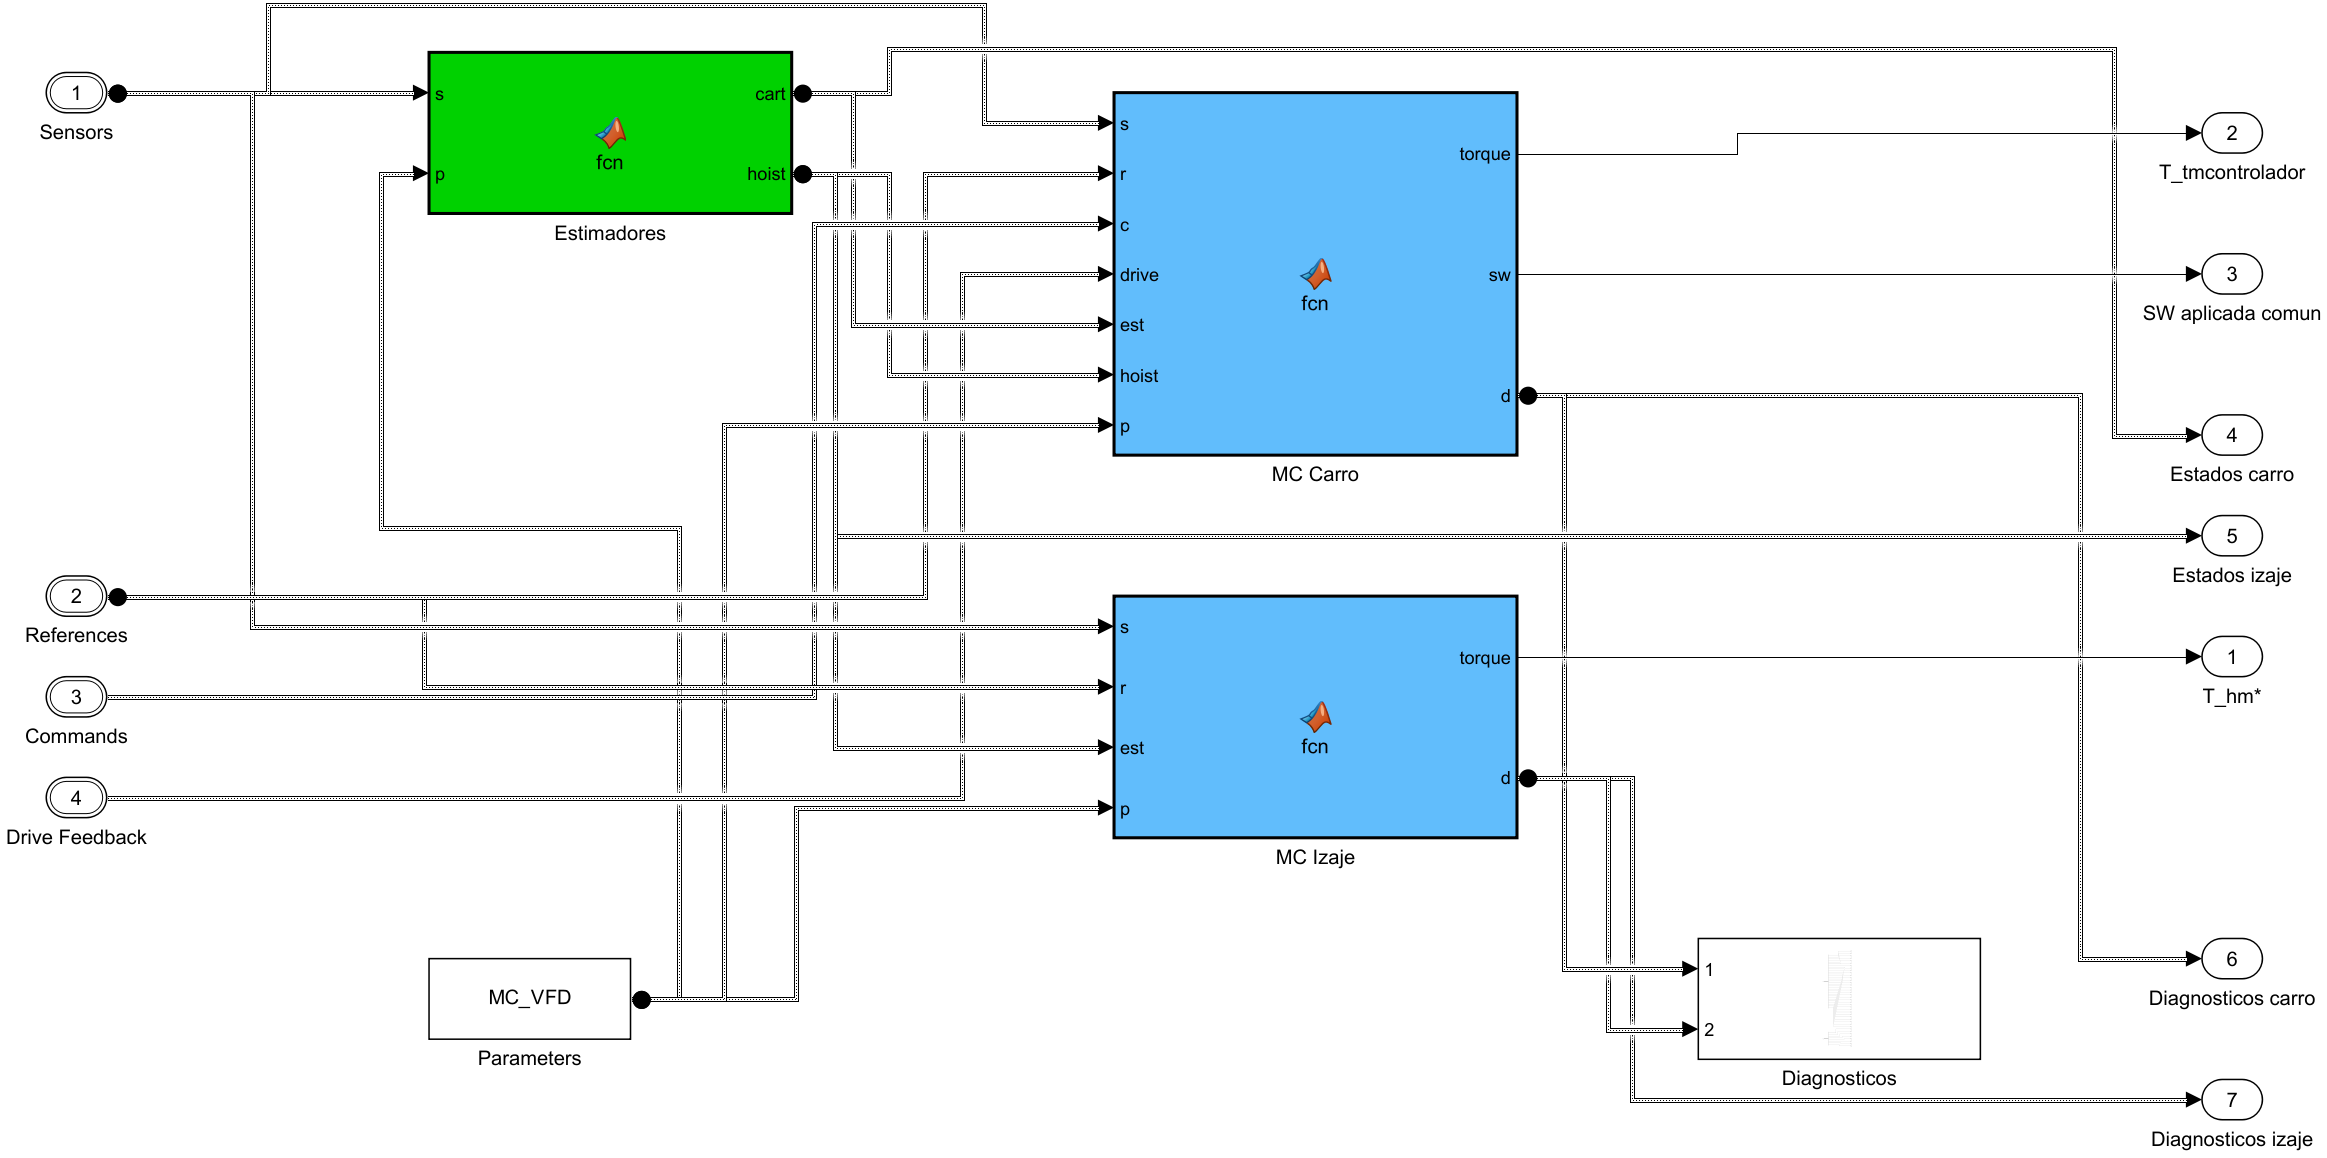
\includegraphics[width=0.99\textwidth,height=0.72\textheight,keepaspectratio]{imagenes_informe/usuario/motionControllerP2/01_estructura_MC.png}
\caption{Organización implementada en Simulink. Los estimadores entregan los estados de ambos ejes; MC Carro y MC Izaje calculan los torques solicitados. Los buses de diagnóstico permiten observar variables internas sin agregar cálculos regulatorios entre las funciones.}
\label{fig:mc_p2_1}
\end{figure}

\Needspace{5\baselineskip}

\subsubsection{Interfaces y parámetros}

Las interfaces se organizan en buses tipados donde cada campo conserva un significado físico y una unidad definida:

\begin{table}[H]
\centering
\caption{Interfaces y parámetros del Motion Controller.}
\label{tab:mc_interfaces}
{\small
\begin{tabular}{@{}L{0.34\textwidth}L{0.60\textwidth}@{}}
\toprule
Interfaz & Contenido principal\\
\midrule
\texttt{Sensors} & Fuerza de cable [N], ángulos de los encoders de motor [rad] y ángulo medido de balanceo [rad]\\
\texttt{References} & Posición, velocidad y aceleración del carro; velocidad y aceleración verticales; transferencia anti-sway existente en las referencias\\
\texttt{Commands} & Habilitación anti-sway \texttt{E} y orden de apertura del freno del carro\\
\texttt{Drive Feedback} & Recorte de torque del carro $\Delta T=T_{lim}-T_{in}$, medido antes de la dinámica del motor y demorado una muestra ($T_s=1$ ms)\\
Parámetros & Geometría, transmisiones, parámetros equivalentes, ganancias, límites, período de muestreo y coeficientes de observadores\\
Salidas & Torques solicitados, corrección anti-sway aplicada, estados cinemáticos y diagnósticos de los dos ejes\\
\bottomrule
\end{tabular}
}
\end{table}

El ángulo de balanceo y la fuerza siguen ingresando como señales del sistema de medición representado en la simulación. Los estimadores incorporados al MC estiman velocidades a partir de encoders. La estimación y validación de la masa del contenedor siguen a cargo del supervisor. La masa equivalente usada en el cálculo del torque es un parámetro del accionamiento, distinto de esa masa estimada.

\Needspace{5\baselineskip}

\subsubsection{Ejecución periódica y memoria}

Las tres funciones se ejecutan con \textbf{T\_s = 1 ms}. Las consignas producidas por el supervisor, cuya actualización es de 20 ms, se retienen entre sus actualizaciones. La interfaz de muestreo no introduce un Unit Delay adicional; la realimentación del recorte de torque conserva su demora original de 1 ms.

La ejecución sigue las relaciones de dependencia en los datos: primero se calculan las estimaciones; luego los módulos regulatorios utilizan las referencias disponibles y los estados estimados.

Esta es también la razón para conservar los estimadores en una función separada dentro del MC. Si se reúnen estimación y regulación en una sola función que recibe las referencias del supervisor, sus salidas de estimación adquieren una dependencia artificial de esas referencias.

\Needspace{5\baselineskip}

\subsection{Realización discreta del controlador seleccionado}

Las leyes regulatorias desarrolladas previamente se implementaron mediante funciones ejecutadas cada $1~\mathrm{ms}$. La conversión conserva los signos, límites, condiciones iniciales y demoras del modelo de bloques. Las operaciones algebraicas se expresan directamente en código y las operaciones dinámicas se representan mediante estados persistentes.

Los observadores mantienen sus estados discretos y la lectura anterior del encoder. El regulador del carro conserva la memoria de anticipación antisway, el factor de habilitación, el estado del integrador limitado y el recorte de aceleración anterior. El regulador del izaje conserva los estados necesarios para sus dos integraciones Tustin.
\Needspace{5\baselineskip}

\subsubsection{Observadores internos de encoder}

Se discretizan los observadores continuos desarrollados en la sección~\ref{sec:observadores-continuos}. Para cada eje, la lectura angular del motor se convierte en ángulo de tambor mediante la relación de transmisión. Se conserva la estructura original, que se reproduce a continuación para establecer la notación de la realización discreta:

\begin{equation}
\dot q=2\zeta\omega_n(u-q)+w,\qquad
\dot w=\omega_n^2(u-q),
\end{equation}

con $u=\theta_m/i$, $\omega_n=40\ \mathrm{rad/s}$ y $\zeta=1$. En forma matricial:

\begin{equation}
\dot{\boldsymbol z}=A\boldsymbol z+Bu,\qquad
\boldsymbol z=\begin{bmatrix}q\\w\end{bmatrix},\quad
A=\begin{bmatrix}-2\zeta\omega_n&1\\-\omega_n^2&0\end{bmatrix},\quad
B=\begin{bmatrix}2\zeta\omega_n\\\omega_n^2\end{bmatrix}.
\end{equation}

La discretización trapezoidal se implementa como:

\begin{equation}
A_d=\left(I-\frac{T_s}{2}A\right)^{-1}\left(I+\frac{T_s}{2}A\right),\qquad
B_d=\left(I-\frac{T_s}{2}A\right)^{-1}\frac{T_s}{2}B,
\end{equation}

\begin{equation}
\boldsymbol z[n]=A_d\boldsymbol z[n-1]+B_d\big(u[n-1]+u[n]\big).
\end{equation}

Los coeficientes se calculan durante la configuración desde los parámetros; cada ejecución utiliza productos y sumas con esos coeficientes. En la primera llamada se entregan los estados iniciales nulos y se registra el encoder, conservando velocidad inicial cero incluso cuando la lectura inicial no sea nula. Los polos discretos nominales tienen módulo aproximadamente 0,960784, inferior a uno.

Las variables cinemáticas mantienen las conversiones originales:

\begin{equation}
x=r_{td}\frac{\theta_{mt}}{i_t},\qquad
\widehat v_t=r_{td}w_t,\qquad
l_h=l_0-\frac{r_{hd}}{2}\frac{\theta_{mh}}{i_h},\qquad
\widehat{\dot l_h}=-\frac{r_{hd}}{2}w_h.
\end{equation}

La posición del carro y la longitud ordenada $l_h$ se obtienen directamente del encoder; el estado $q$ no las reemplaza. Esta longitud cinemática $l_h$ es distinta de la longitud geométrica deformada $l$ de la planta. La regulación utiliza $l_h$ para su ganancia pendular; la elasticidad se representa mediante la diferencia $l-l_h$ en el modelo del cable. Se conserva el factor de reeving del izaje y la convención de signos empleada en el modelo.

\Needspace{5\baselineskip}

\subsubsection{Función regulatoria del carro}

En cada muestra se calcula la referencia angular de \eqref{eq:antisway} y se actualiza la anticipación limitada desarrollada en la sección~\ref{sec:integracion_p1}. Luego se forma la corrección antisway y se obtiene la consigna efectiva de velocidad. Con el error de velocidad y los recortes anteriores se calcula la salida integral; posteriormente se limita la aceleración total, se obtiene el torque solicitado y se actualizan las memorias para la siguiente muestra.

En el código, \texttt{s.theta} representa $\theta_l$, \texttt{thetaRef} representa $\theta_{ref}$ y \texttt{est.length} corresponde a $l_h$. La actualización de la memoria anticipativa es
\begin{equation}
b^*[n]=-2\zeta\omega_{p,f}[n]l_f[n]\theta_{ref}[n],\qquad
b[n]=b[n-1]+\operatorname{sat}_{\rho T_s}\big(b^*[n]-b[n-1]\big),
\end{equation}
con $\rho=0{,}25~\mathrm{m/s^2}$, $l_f=\max(1~\mathrm{m},l_h)$ y $\omega_{p,f}=\sqrt{g_0/l_f}$, donde $g_0=9{,}80665~\mathrm{m/s^2}$ y $\zeta=1$. La realimentación conserva $\omega_p=\sqrt{g/l_h}$.

Con \texttt{E} habilitado y orden de freno abierta, se actualiza el factor de incorporación y se aplica
\begin{align}
\alpha[n]&=\min\left(1,\alpha[n-1]+\frac{T_s}{2~\mathrm{s}}\right),\\
v_{sw}[n]&=\operatorname{sat}_{3.2}\left(\alpha[n]\big(2\zeta\omega_p[n]l_h[n]\theta_l[n]+b[n]\big)\right).
\end{align}
Al deshabilitar la corrección o recibir orden de freno cerrado se anulan $b$, $\alpha$ y $v_{sw}$. El límite $\rho$ actúa sobre la pendiente de la contribución anticipativa de velocidad; la anticipación de aceleración $a_{ref}$ permanece en la suma del PI.

La consigna efectiva de velocidad y su error se obtienen mediante
\begin{align}
v^*[n]&=v_{ref}[n]+v_{sw}[n]+v_{transfer}[n]+K_x(x_{ref}[n]-x[n]),\\
v_d[n]&=\operatorname{sat}_{v_{max}}(v^*[n]),\qquad e_v[n]=v_d[n]-\widehat v_t[n].
\end{align}
El término $v_{transfer}$ conserva la transferencia incorporada en las referencias. La entrada integral utiliza los recortes de la muestra anterior:
\begin{equation}
u_I[n]=e_v[n]+\frac{1}{K_iT_{aw}}\left(\Delta a[n-1]+\frac{i_t}{r_{td}M_{EQt}}\Delta T[n-1]\right),\qquad T_{aw}=1~\mathrm{s}.
\end{equation}
Aquí $\Delta a=a_{cmd}-a^*$ y $\Delta T=T_{lim}-T_{in}$, medido antes de la dinámica del motor y demorado $1~\mathrm{ms}$ por la interfaz. $K_p$ y $K_i$ corresponden a $K_{pv}$ y $K_{iv}$. La recurrencia conserva los dos medios pasos limitados del bloque Tustin:
\begin{align}
I[n]&=\operatorname{sat}_{I_{max}}\left(X[n]+\frac{T_s}{2}u_I[n]\right),\\
X[n+1]&=\operatorname{sat}_{I_{max}}\left(I[n]+\frac{T_s}{2}u_I[n]\right),\qquad I_{max}=\frac{a_{max}}{K_i}=4~\mathrm{m}.
\end{align}
Se calcula primero la salida $I[n]$ y luego su memoria $X[n+1]$, conservando el comportamiento del integrador al entrar y salir de saturación. El mando y el torque resultan
\begin{align}
a^*[n]&=a_{ref}[n]+K_p e_v[n]+K_i I[n],\\
a_{cmd}[n]&=\operatorname{sat}_{0.8}(a^*[n]),\\
T_t^*[n]&=\frac{r_{td}M_{EQt}}{i_t}\left(a_{cmd}[n]+\frac{b_{EQt}}{M_{EQt}}\widehat v_t[n]-\frac{2F_w[n]\sin\theta_l[n]}{M_{EQt}}\right).
\end{align}
La compensación horizontal utiliza el ángulo medido y permanece activa con \texttt{E=0}. La autorización y el recorte final de torque se mantienen fuera de la función regulatoria.
\Needspace{5\baselineskip}

\subsubsection{Función regulatoria del izaje}

Las referencias verticales del supervisor se convierten a la convención de longitud: $v_{l,ref}=-v_{h,ref}$ y $a_{l,ref}=-a_{h,ref}$. El error es $e_h=v_{l,ref}-\widehat{\dot l_h}$. Se mantienen los dos integradores Tustin:

\begin{equation}
z_1[n]=z_1[n-1]+\frac{T_s}{2}(e_h[n-1]+e_h[n]),
\end{equation}

\begin{equation}
z_2[n]=z_2[n-1]+\frac{T_s}{2}(z_1[n-1]+z_1[n]).
\end{equation}

Con la convención de fuerza del modelo, el torque solicitado se conserva como:

\begin{equation}
T_h^*[n]=K_{hi}z_2[n]+K_{hp}z_1[n]+K_{hd}e_h[n]
-\frac{r_{hd}}{i_h}\left(M_{EQh}a_{l,ref}[n]+b_{EQh}v_{l,ref}[n]\right)
+\frac{r_{hd}}{i_h}F_w[n].
\end{equation}

La codificación concentra las conversiones de signo y el cálculo de torque en la función del eje. Conserva la regulación original y no incorpora un anti-windup nuevo al izaje. La coordinación del freno, la toma, la entrega y el pesaje siguen resueltas por el supervisor.

\Needspace{5\baselineskip}

\subsubsection{Correspondencia entre bloques y código}

\begin{table}[H]
\centering
{\small
\begin{tabular}{@{}L{0.34\textwidth}L{0.60\textwidth}@{}}
\toprule
Elemento del modelo de bloques & Representación en el MC\\
\midrule
Ganancia, suma y funciones trigonométricas & Expresiones algebraicas dentro de la función del eje\\
Saturación & Operación \texttt{min}/\texttt{max} con el límite correspondiente\\
Integrador Tustin & Recurrencia explícita con estado persistente\\
Memoria del recorte de aceleración & Variable persistente actualizada al finalizar el cálculo\\
Observador continuo de encoder & Recurrencia matricial Tustin con estados persistentes\\
Incorporación del anti-sway & Estado persistente de habilitación y condición de inhibición\\
Conexiones entre módulos & Buses con campos y tipos definidos\\
\bottomrule
\end{tabular}
}
\end{table}

La conversión preserva el orden de operaciones, los signos, los estados iniciales y las demoras. Esos detalles son parte de la equivalencia: reemplazar un integrador limitado por una integral aparentemente similar, o añadir una muestra de retardo para simplificar las conexiones, puede modificar el transitorio aun conservando las ganancias nominales.

\Needspace{5\baselineskip}

\subsection{Verificación de la implementación}

La verificación se centra en comprobar que el MC conserva la regulación y el desempeño de su equivalente en bloques. Para ello, primero se contrasta el cálculo del regulador y luego se comparan ambas implementaciones durante una maniobra completa. Finalmente, se revisa si el MC reproduce la mejora obtenida al limitar la anticipación anti-sway.

En primera instancia, se comparó el MC con el sistema de \textbf{bloques FF limitado}, suministrando las mismas referencias y estimaciones a ambos reguladores. Esta prueba permite comprobar la correspondencia entre las ecuaciones implementadas mediante bloques y su expresión en código, antes de evaluar el efecto de los estimadores discretos sobre el ciclo completo. Una vez verificada la regulación, se ejecutó la misma maniobra completa con el modelo de bloques y con el MC final.

\Needspace{5\baselineskip}

\FloatBarrier
\Needspace{16\baselineskip}
\subsubsection{Equivalencia entre MC FF y bloques FF en la maniobra completa}

La siguiente tabla resume las máximas diferencias entre las señales de ambas simulaciones y permite apreciar el efecto de este cambio sobre el comportamiento del sistema.

\begin{table}[H]
\centering
{\small
\begin{tabular}{@{}L{0.34\textwidth}L{0.60\textwidth}@{}}
\toprule
Magnitud & MC FF frente a bloques FF\\
\midrule
Series comunes comparadas & 137\\
Diferencia máxima de posición del carro & 0,085109 mm\\
Diferencia máxima de altura de carga & 0,677645 mm\\
Diferencia máxima de ángulo & 0,000145257\ensuremath{^{\circ}}\\
Diferencia máxima de torque solicitado del carro & 0,0441535 Nm\\
Diferencia máxima de torque solicitado del izaje & 29,396394 Nm\\
Diferencia máxima de tiempos de fase & 0 s\\
Duración de la corrida de bloques FF & 381,398333 s\\
Duración de la corrida MC FF & 381,399 s\\
\bottomrule
\end{tabular}
}
\end{table}


\begin{figure}[H]
\centering
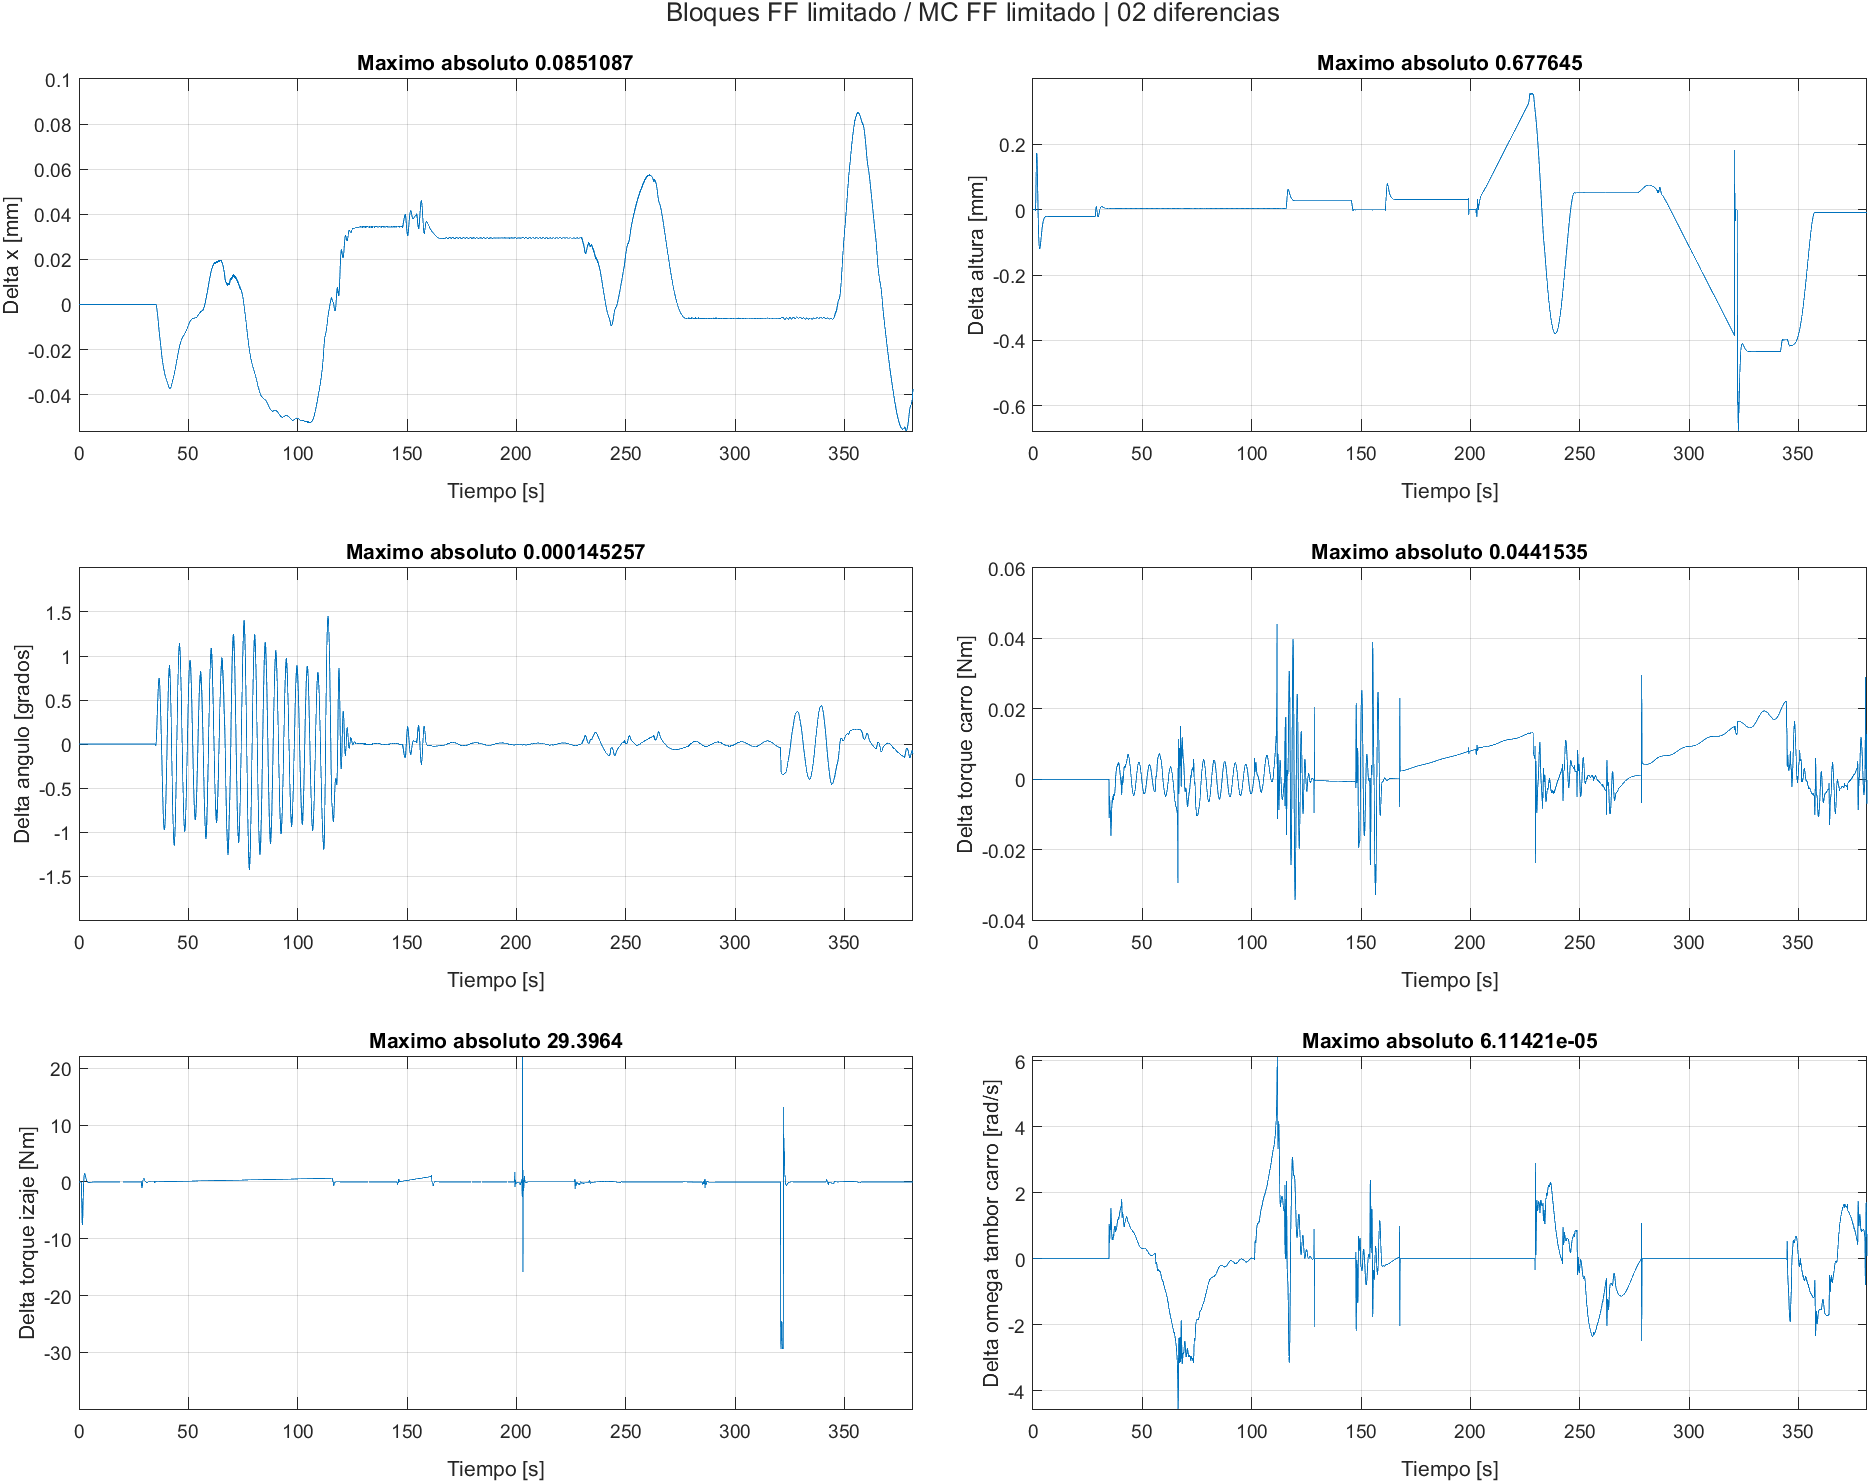
\includegraphics[width=0.99\textwidth,height=0.72\textheight,keepaspectratio]{imagenes_informe/usuario/motionControllerP2/03_diferencias_MC_FF.png}
\caption{Diferencias entre el MC final y el modelo de bloques con la misma ley de anticipación limitada. Las escalas permiten apreciar las pequeñas diferencias del ciclo cerrado, asociadas a la discretización y a la integración numérica.}
\label{fig:mc_p2_2}
\end{figure}

\Needspace{5\baselineskip}

\subsubsection{Conservación del resultado de desempeño}

Además de comparar las señales, se comprobó que la implementación en código conserva el resultado de desempeño analizado en la sección~\ref{sec:integracion_p1}. Con la ley simple, la aceleración física máxima del carro es \textbf{1,453512 m/s\textsuperscript{2}} en bloques y \textbf{1,453490 m/s\textsuperscript{2}} en el MC. La proximidad de estos valores confirma que la conversión reproduce también el transitorio de la ley original.

Al incorporar la anticipación limitada, el máximo físico global se reduce a \textbf{0,627412 m/s\textsuperscript{2}} en bloques y \textbf{0,627371 m/s\textsuperscript{2}} en el MC. La \cref{fig:mc_p2_3} muestra cómo ambas implementaciones reproducen la reducción del pico durante la parada manual.

En el MC final, el máximo de $|a_{cmd}|$ es \textbf{0,505180 m/s\textsuperscript{2}}, y durante la maniobra no se observó recorte de torque del carro. También se verificó el límite de variación de la anticipación de \textbf{0,25 m/s\textsuperscript{2}} durante las muestras habilitadas, junto con residuos nulos en las ecuaciones de realimentación y suma de anti-sway.


\begin{figure}[H]
\centering
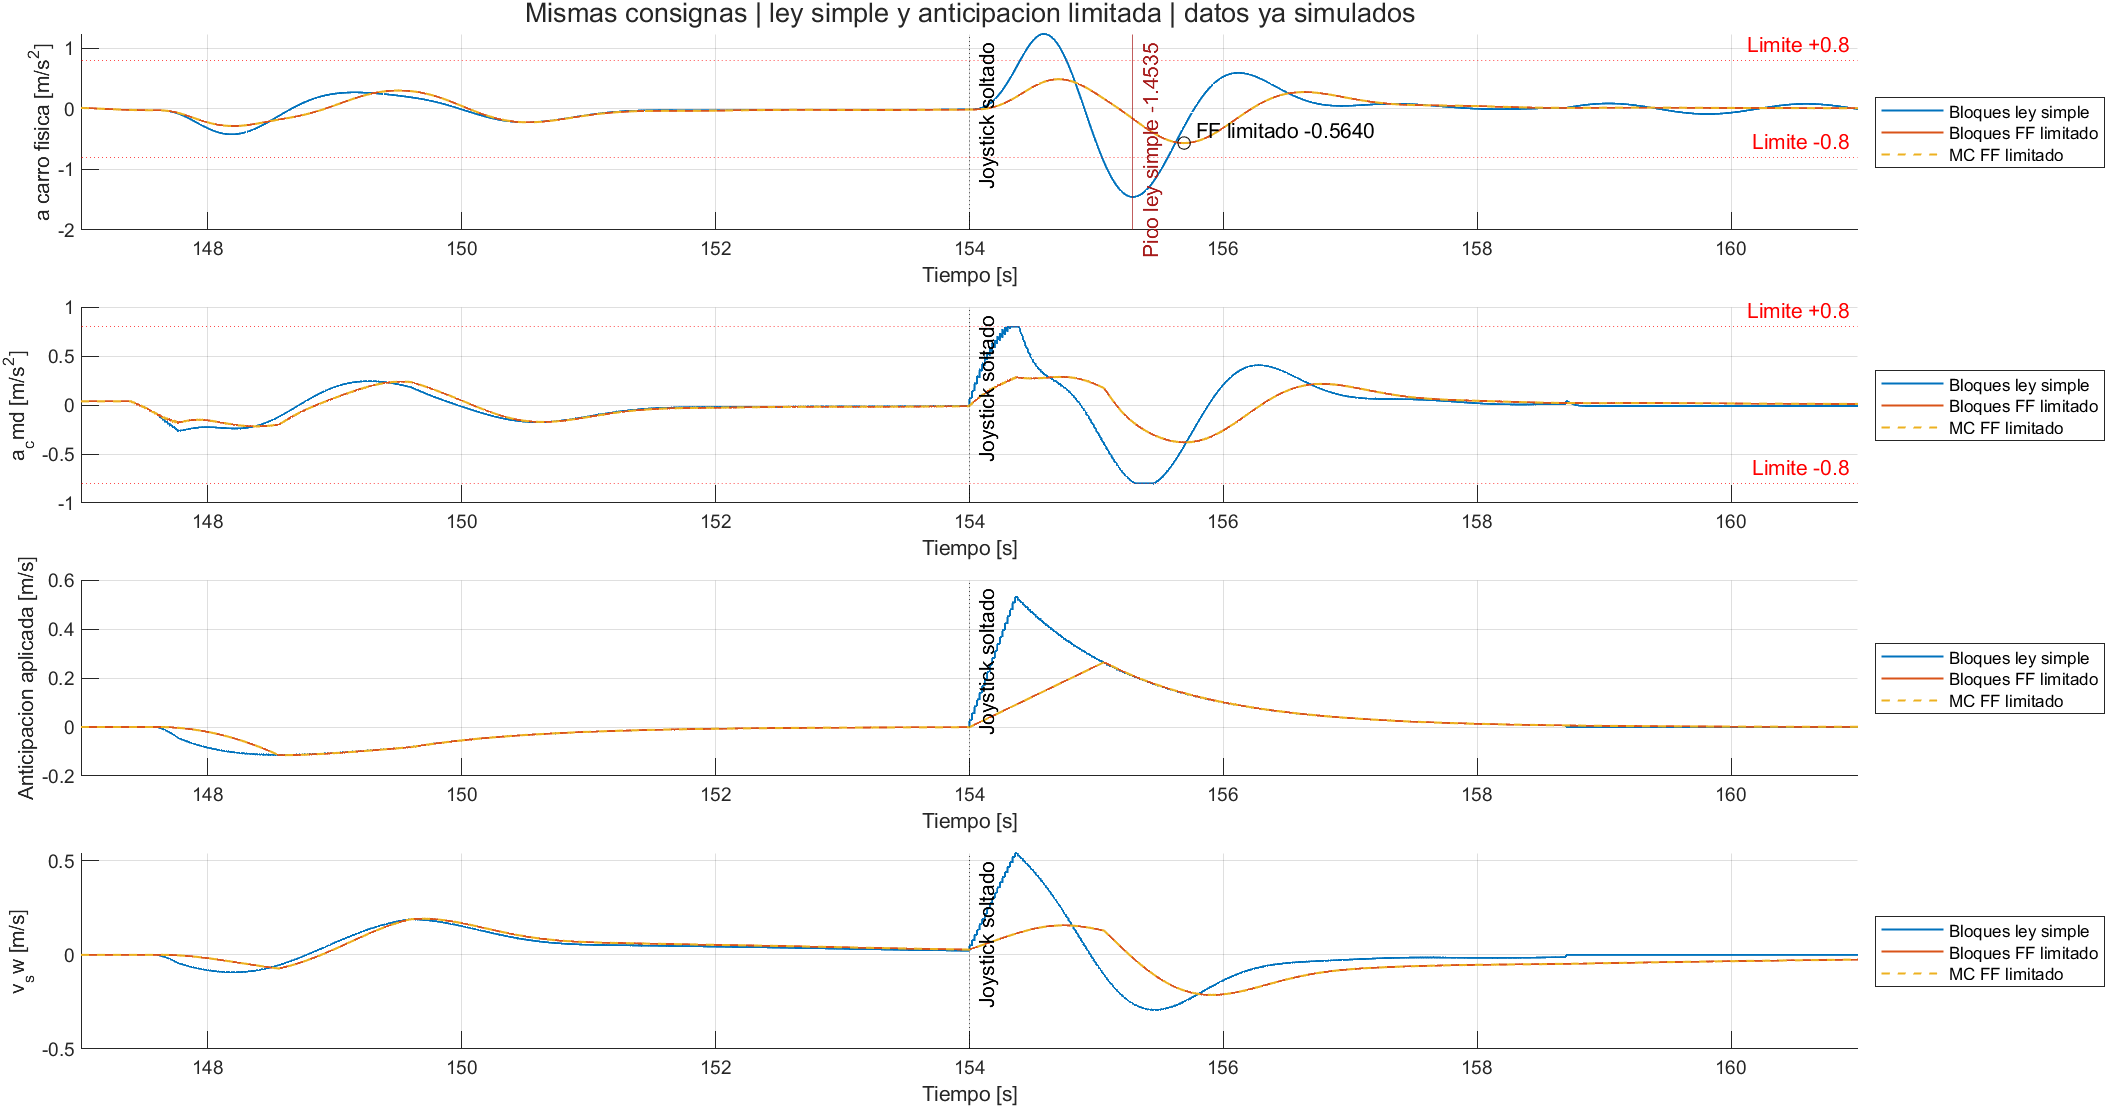
\includegraphics[width=0.99\textwidth,height=0.72\textheight,keepaspectratio]{imagenes_informe/usuario/motionControllerP2/04_transitorio_manual.png}
\caption{Transitorio tras la retirada del joystick: ley simple, bloques con FF limitado y MC con FF limitado. Se conservan los tiempos absolutos de las corridas. El MC final reproduce el acondicionamiento de anticipación y la reducción de excitación observados en bloques.}
\label{fig:mc_p2_3}
\end{figure}

Estos resultados respaldan la equivalencia del MC para la maniobra ensayada y muestran que conserva la mejora obtenida con la anticipación limitada. Su alcance corresponde a ese ensayo; los transitorios de contacto y freno del izaje permanecen como en el modelo de referencia. La justificación mecánica de la modificación se desarrolla en el apartado de integración de la sección~\ref{sec:integracion_p1}.

\par
\Needspace{10\baselineskip}
\section{Pruebas del sistema: MIL y SIL}
\label{sec:pruebas_sistema}
\label{sec:pruebas_SIL}
Se reúnen las pruebas específicas del autómata de seguridad en Stateflow, el ciclo completo ejecutado íntegramente en Simulink (MIL) y los ensayos de medio ciclo con los autómatas en CODESYS (SIL), seguidos de sus comparativas y límites de validación. Cada apartado identifica la arquitectura y el alcance efectivamente ensayados. La verificación específica de equivalencia del MC se conserva en la sección~\ref{sec:mc_p2}; la prueba completa CODESYS--MC--planta cierra esta sección con relevamiento y dos transferencias físicas confirmadas (apartado~\ref{subsec:prueba_completa_codesys}).

% Síntesis del banco aislado; resultados preservados y figuras retiradas del documento.
\Needspace{5\baselineskip}
\subsection{Validación funcional del autómata de seguridad en Stateflow}
\label{sec:validacion_seguridad_stateflow}
Se evaluó una copia del subsistema de seguridad mediante \textbf{25 escenarios de prueba seleccionados} para evaluar la respuesta del autómata de seguridad ante límites de posición, sobrevelocidad, parada de emergencia, pérdida de comunicación y solicitudes de reinicio. También se estudiaron fallas sucesivas, fallas simultáneas y condiciones peligrosas presentes desde el arranque.

Las pruebas se realizaron sobre el subsistema de seguridad aislado, mediante entradas programadas y con un período de ejecución de $20~\mathrm{ms}$. Se verificaron los permisos de movimiento y las autorizaciones de apertura de los frenos, sin incluir la respuesta mecánica de la planta. La \cref{tab:resumen_pruebas_seguridad} resume los principales resultados.

\begin{table}[!htb]
	\centering
	\small
	\renewcommand{\arraystretch}{1.2}
	\caption{Resumen de los resultados de las pruebas del autómata de seguridad.}
	\label{tab:resumen_pruebas_seguridad}
	\begin{tabular}{L{0.26\textwidth}L{0.66\textwidth}}
		\toprule
		\textbf{Aspecto evaluado} & \textbf{Resultado observado} \\
		\midrule
		
		Límites y sobrevelocidad &
		Los sensores se activaron al alcanzar el umbral, incluida la igualdad. \\
		
		Retención y reinicio &
		La emergencia permaneció enclavada después de retirar la causa. Un nuevo flanco de reinicio permitió recuperar los permisos cuando se cumplieron las condiciones correspondientes. \\
		
		Fallas sucesivas en ambos ejes &
		La segunda falla provocó el escalamiento a emergencia total. \\
		
		Fallas simultáneas en ambos ejes &
		Prevaleció la emergencia de izaje y el carro conservó su permiso. La prioridad de las transiciones y la detección por flanco impidieron reconocer posteriormente la falla horizontal. \\
		
		Pérdida del latido de comunicación &
		El watchdog detectó el vencimiento de los $5~\mathrm{s}$ sin cambios del latido. La emergencia total se activó $20~\mathrm{ms}$ después, debido al orden de ejecución de las regiones. \\
		
		Recuperación del watchdog &
		Fueron necesarios dos flancos de reinicio: uno para borrar la falla y otro para liberar la emergencia. Sin restablecer el latido, el fallo volvió a aparecer cinco segundos después. \\
		
		Fallas presentes al arrancar &
		Los límites y la sobrevelocidad inicialmente activos no provocaron intervención, porque la lógica esperaba un nuevo flanco. El pulsador, evaluado por nivel, sí produjo emergencia total. \\
		
		\bottomrule
	\end{tabular}
\end{table}

Los ensayos confirmaron la respuesta prevista ante las condiciones habituales y permitieron identificar limitaciones en la detección de fallas simultáneas, la protección durante el arranque y la recuperación del watchdog.

\par

\Needspace{5\baselineskip}

\subsection{Prueba completa en Simulink (MIL)}
\label{subsec:prueba_completa_MIL}

Se ensayó en una única corrida el relevamiento LiDAR y dos transferencias consecutivas en sentidos opuestos. La planta, el controlador de movimiento, el supervisor y el nivel de seguridad se ejecutaron íntegramente en Simulink.

La primera transferencia llevó un contenedor del centro del muelle, \textit{slot} 6 ($x=-16.58~\mathrm{m}$), al centro del barco, \textit{slot} 23 ($x=24.90~\mathrm{m}$). Después se desplazó el conjunto vacío al extremo derecho operable del barco, \textit{slot} 32 ($x=46.86~\mathrm{m}$), y se trasladó otro contenedor al extremo izquierdo del muelle, \textit{slot} 1 ($x=-28.78~\mathrm{m}$). La duración total fue de $626.36~\mathrm{s}$.

Los posicionamientos se solicitaron en automático. Las tomas, aproximaciones finales de apoyo y extracciones verticales se realizaron mediante los mandos proporcionales de la HMI, respetando los permisos y retenciones del supervisor. El controlador antisway conservó su realimentación angular, su anticipación limitada y su rampa de habilitación.

\Needspace{5\baselineskip}

\FloatBarrier
\Needspace{16\baselineskip}
\subsubsection{Cronología de las dos transferencias}

\Needspace{12\baselineskip}
\begin{longtable}{C{1.6cm} C{1.0cm} L{6.4cm} L{4.4cm}}

\caption{Eventos efectivos de la prueba completa MIL.}\label{tab:cronologia_completa_MIL}\\

\toprule Tiempo [s] & Tramo & Evento & Destino\\\midrule\endfirsthead

\toprule Tiempo [s] & Tramo & Evento & Destino\\\midrule\endhead

$0.24$ & 1 & Arranque & Toma en muelle\\

$0.40$ & 1 & Inicio del barrido & Toma en muelle\\

$114.64$ & 1 & Extracción y despeje local & Toma en muelle\\

$116.68$ & 1 & Solicitud de posicionamiento automático & Toma en muelle\\

$116.76$ & 1 & Posicionamiento automático efectivo & Toma en muelle\\

$138.88$ & 1 & Solicitud de aproximación final manual & Toma en muelle\\

$142.84$ & 1 & Descenso final & Toma en muelle\\

$192.12$ & 1 & Contacto y solicitud de twistlocks & Toma en muelle\\

$193.16$ & 2 & Extracción y despeje local & Entrega en barco\\

$194.96$ & 1 & Toma física confirmada & Toma en muelle\\

$206.80$ & 2 & Solicitud de posicionamiento automático & Entrega en barco\\

$206.88$ & 2 & Posicionamiento automático efectivo & Entrega en barco\\

$270.84$ & 2 & Solicitud de aproximación final manual & Entrega en barco\\

$273.24$ & 2 & Descenso final & Entrega en barco\\

$308.60$ & 2 & Contacto y solicitud de twistlocks & Entrega en barco\\

$309.00$ & 3 & Extracción y despeje local & Toma en barco\\

$309.00$ & 2 & Entrega física confirmada & Entrega en barco\\

$347.88$ & 3 & Solicitud de posicionamiento automático & Toma en barco\\

$347.96$ & 3 & Posicionamiento automático efectivo & Toma en barco\\

$375.92$ & 3 & Solicitud de aproximación final manual & Toma en barco\\

$379.52$ & 3 & Descenso final & Toma en barco\\

$444.72$ & 3 & Contacto y solicitud de twistlocks & Toma en barco\\

$445.76$ & 4 & Extracción y despeje local & Entrega en muelle\\

$447.56$ & 3 & Toma física confirmada & Toma en barco\\

$510.88$ & 4 & Solicitud de posicionamiento automático & Entrega en muelle\\

$510.96$ & 4 & Posicionamiento automático efectivo & Entrega en muelle\\

$612.88$ & 4 & Solicitud de aproximación final manual & Entrega en muelle\\

$615.28$ & 4 & Descenso final & Entrega en muelle\\

$623.88$ & 4 & Contacto y solicitud de twistlocks & Entrega en muelle\\

$624.32$ & 4 & Entrega física confirmada & Entrega en muelle\\

$624.32$ & 4 & Solicitud de parada final & Entrega en muelle\\

$626.36$ & 4 & Parada normal confirmada & Entrega en muelle\\
\bottomrule\end{longtable}

\Needspace{5\baselineskip}

\subsubsection{Relevamiento y actualización del perfil}

El barrido precedió a ambas tomas. La comparación del perfil relevado con el perfil físico inicial de los slots operables produjo un error máximo de $0.000000~\mathrm{m}$. Los slots no operables se excluyen de esa métrica, porque su cota neutra no representa una superficie de toma o entrega.

El perfil final conserva el balance de los dos contenedores: disminuye $2.59~\mathrm{m}$ en los slots 6 y 32 y aumenta la misma altura en los slots 23 y 1. La figura muestra los puntos LiDAR y el perfil reconstruido antes de las transferencias, e identifica las dos tomas y sus destinos. Los cambios posteriores se comprueban en el perfil final registrado.

\begin{figure}[H]
\centering
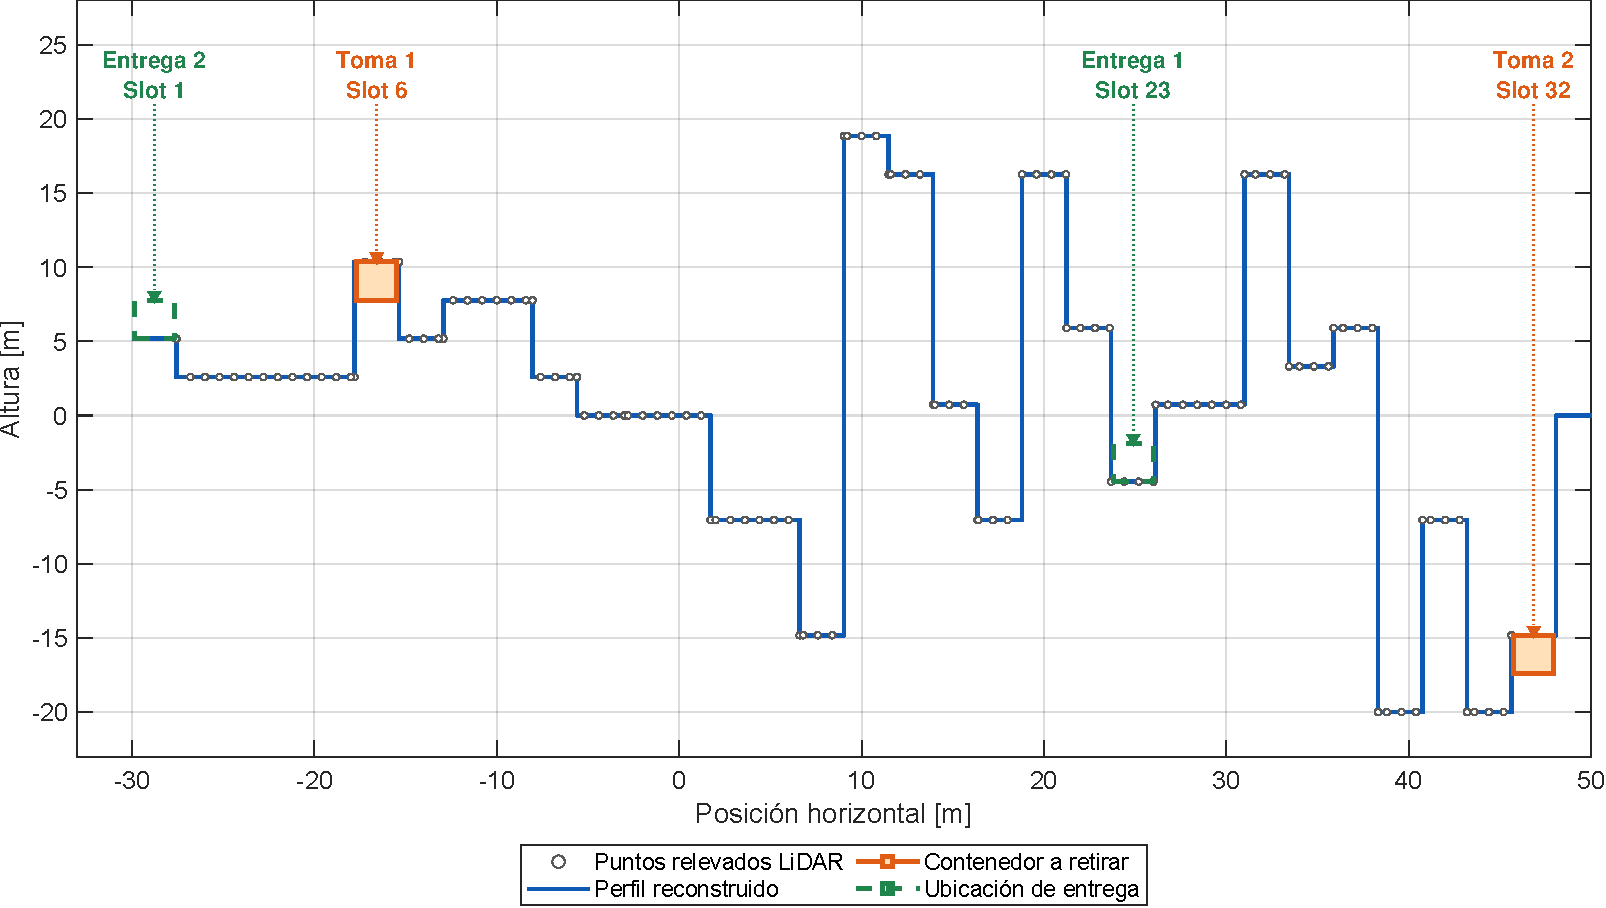
\includegraphics[width=0.98\textwidth]{imagenes_informe/prueba_completa_MIL/perfil.pdf}
\caption{Relevamiento LiDAR y perfil reconstruido. Se identifican los contenedores a retirar (slots 6 y 32) y sus ubicaciones de entrega (slots 23 y 1).}
\label{fig:completa_MIL_perfil}
\end{figure}





\begin{figure}[H]
\centering
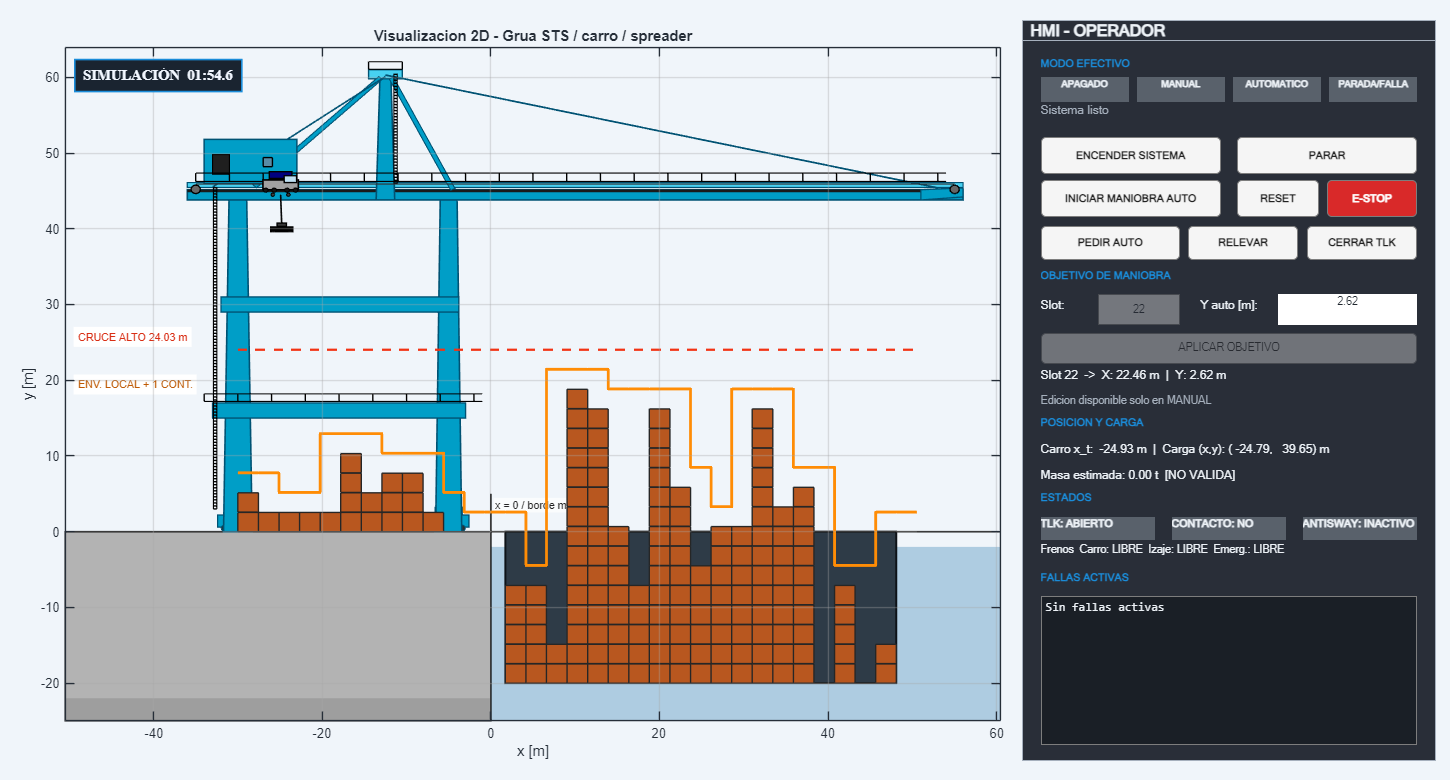
\includegraphics[width=0.98\textwidth]{imagenes_informe/prueba_completa_MIL/01_barrido.png}
\caption{Visualización y HMI al finalizar el barrido real.}
\label{fig:completa_MIL_01_barrido}
\end{figure}


\par
\Needspace{5\baselineskip}
\subsubsection{Dinámica del carro y seguimiento horizontal}

La figura reúne posición, velocidad y aceleración del carro, comparadas con sus referencias. La posición y la velocidad se reconstruyen a partir del encoder del accionamiento; la aceleración se calcula como derivada numérica de esa velocidad, utilizando los tiempos del registro y sin filtrado adicional. Así se observa el seguimiento del accionamiento sin superponer la respuesta elástica de la carga.

Las franjas sombreadas delimitan las dos transferencias cargadas, desde la toma confirmada hasta la entrega confirmada. Las líneas verticales identifican los contactos de toma y apoyo. Entre ambas franjas se desarrolla el reposicionamiento del spreader vacío hacia la segunda toma.

\begin{figure}[H]
\centering
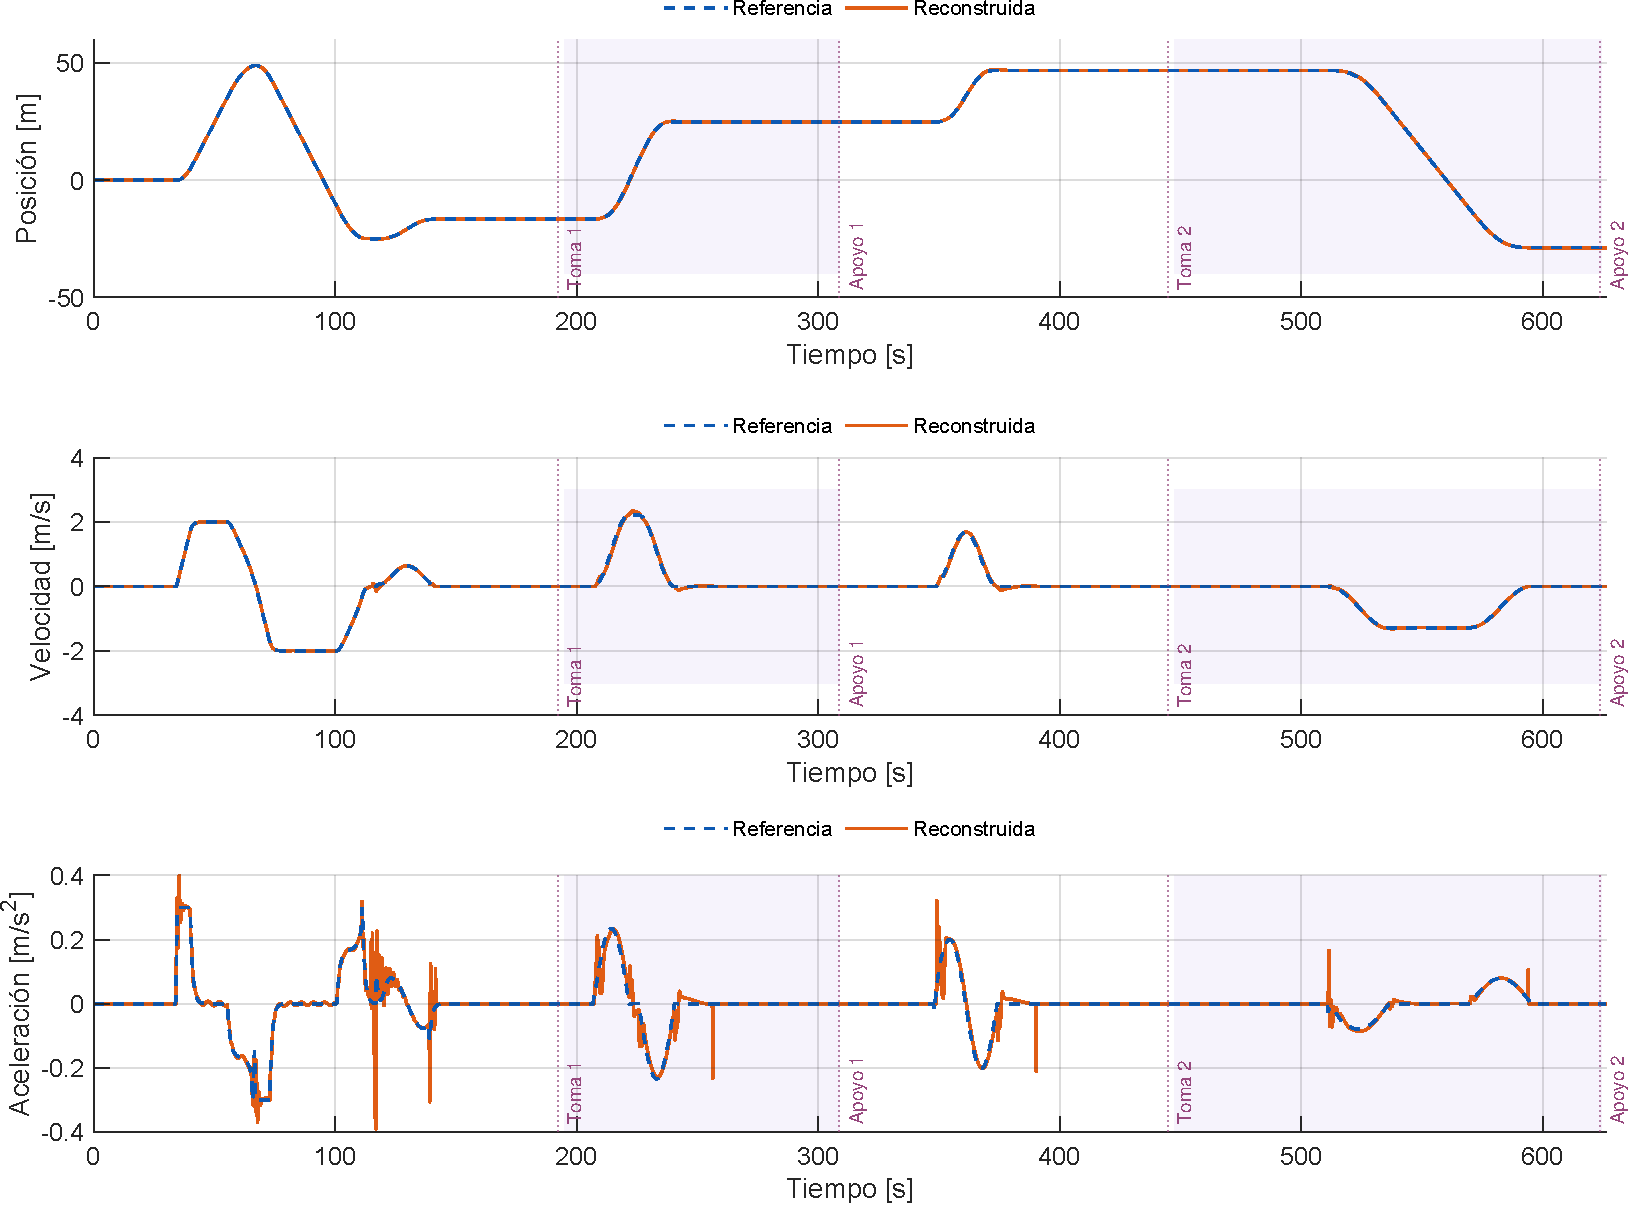
\includegraphics[width=0.98\textwidth]{imagenes_informe/prueba_completa_MIL/paneles_0810/carro_tres_filas.pdf}
\caption{Seguimiento horizontal: posición, velocidad y aceleración reconstruidas frente a sus referencias. Las franjas indican las transferencias cargadas y las líneas verticales, los contactos de toma y apoyo.}
\label{fig:completa_MIL_carro_panel}
\end{figure}

\par
\Needspace{5\baselineskip}
\subsubsection{Izaje, contacto y entrega física}

El panel de izaje reúne las mismas tres magnitudes. La altura se infiere del accionamiento mediante $\widehat y_h=Y_{t0}-\widehat l_h$, con $Y_{t0}=45~\mathrm{m}$; la velocidad vertical es $-\dot{\widehat l}_h$ y la aceleración se obtiene de su derivada numérica. Esta altura representa la posición inferida del accionamiento y no la altura geométrica deformada de la carga.

Los contactos de las entregas se registraron a los $308.60$ y $623.88~\mathrm{s}$; sus confirmaciones se produjeron a los $309.00$ y $624.32~\mathrm{s}$. Por ello, contacto, apertura de twistlocks y confirmación de entrega se consideran eventos distintos.

\begin{figure}[H]
\centering
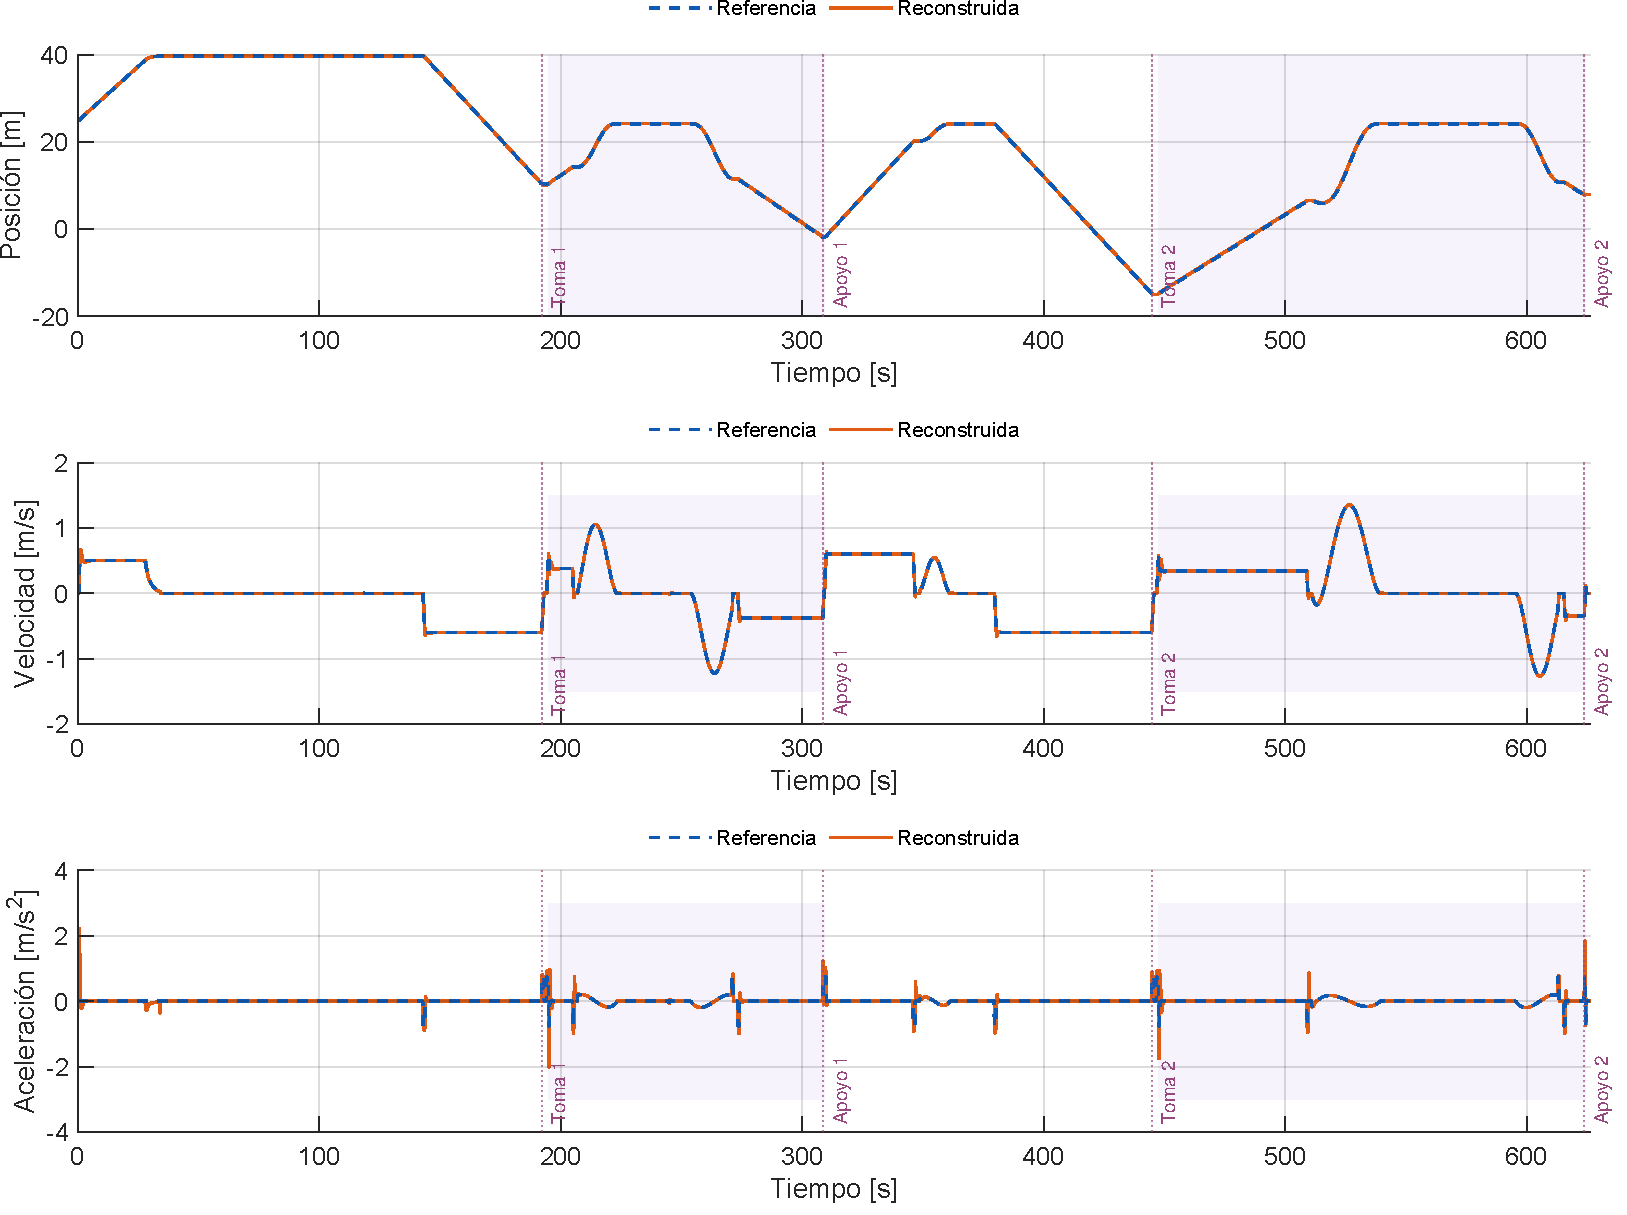
\includegraphics[width=0.98\textwidth]{imagenes_informe/prueba_completa_MIL/paneles_0810/izaje_tres_filas.pdf}
\caption{Seguimiento del izaje: altura inferida del accionamiento, velocidad y aceleración reconstruidas, comparadas con sus referencias.}
\label{fig:completa_MIL_izaje_panel}
\end{figure}

La planta conserva un máximo de aceleración vertical física de $149.77~\mathrm{m/s^2}$ a los $624.04~\mathrm{s}$, durante el transitorio de apoyo y liberación. Ese extremo corresponde a la dinámica física de la carga, no a la aceleración reconstruida del accionamiento. Su análisis requiere considerar conjuntamente el contacto y la elasticidad; no se incorpora a la escala de este panel.

\par
\Needspace{5\baselineskip}
\subsubsection{Balanceo y acción antisway}

El ángulo se compara con su referencia en dos intervalos: el barrido, hasta los $112.00~\mathrm{s}$, y las aproximaciones y transferencias posteriores. La separación corresponde a la desactivación de la señal de barrido; cada fila utiliza una escala propia para que sus transitorios no oculten el balanceo durante el transporte. La curva sensada corresponde al sensor angular utilizado en la simulación.

Durante el traslado automático cargado hacia el barco, entre $206.88$ y $270.84~\mathrm{s}$, el máximo absoluto del ángulo fue de $0.0273~\mathrm{rad}$. Durante el traslado cargado hacia el muelle, entre $510.96$ y $612.88~\mathrm{s}$, fue de $0.0094~\mathrm{rad}$.

\begin{figure}[H]
\centering
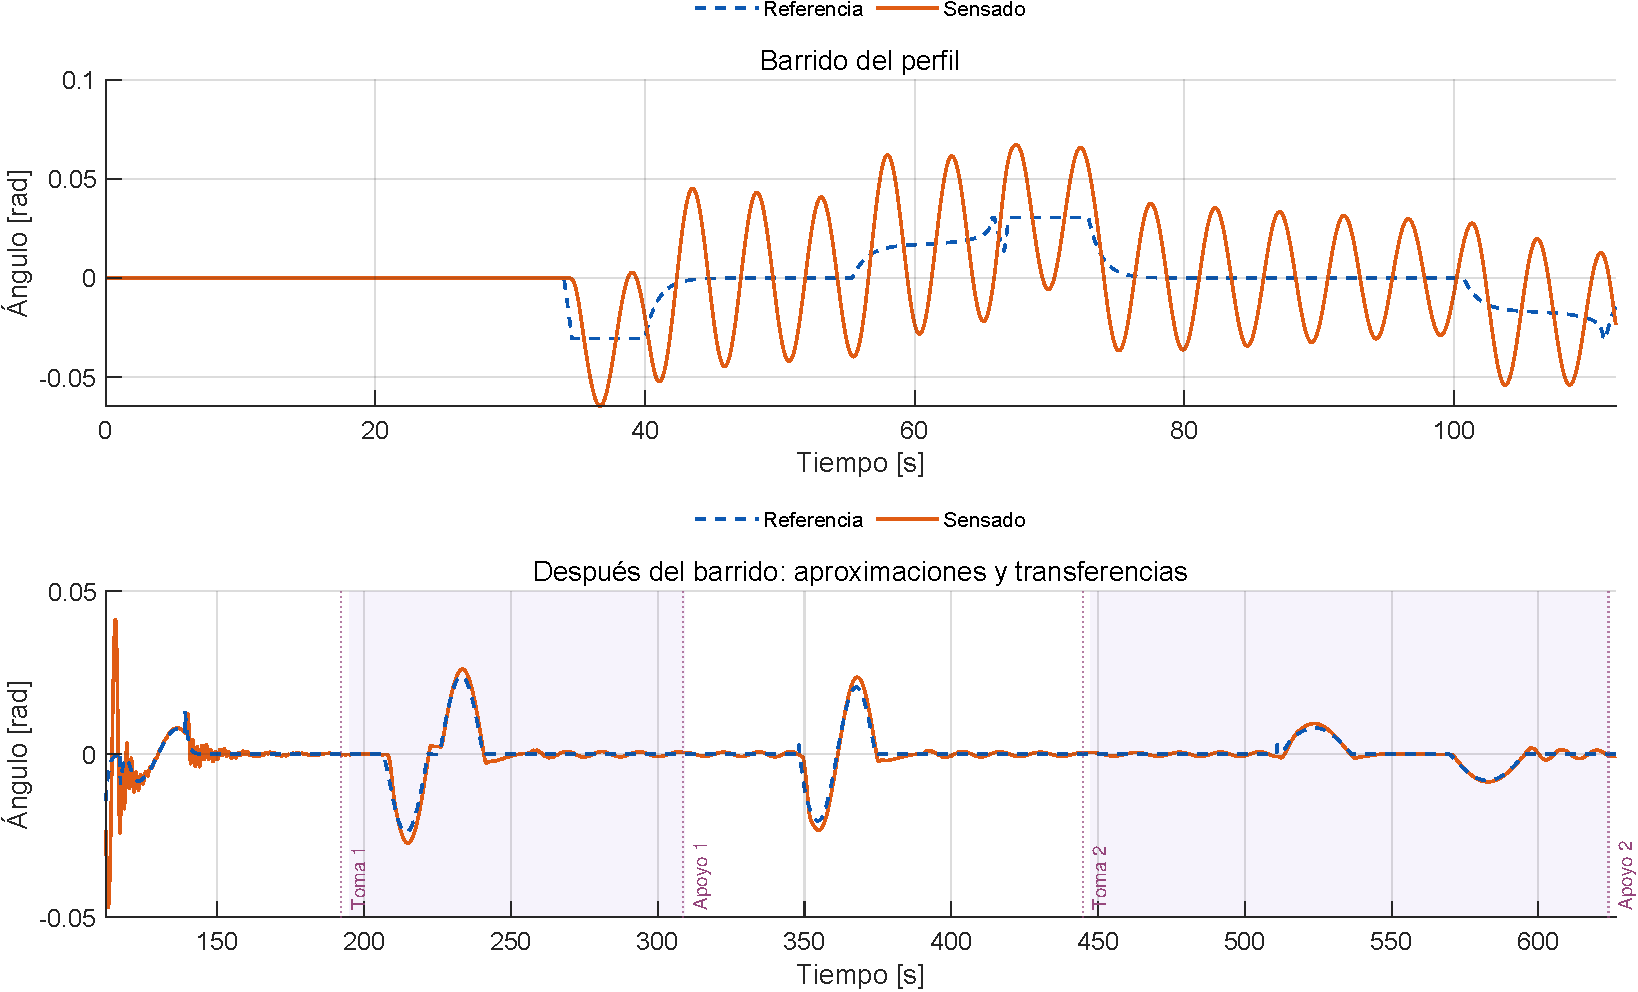
\includegraphics[width=0.98\textwidth]{imagenes_informe/prueba_completa_MIL/paneles_0810/angulo_dos_etapas.pdf}
\caption{Ángulo de referencia y sensado durante el barrido (arriba) y durante las maniobras posteriores (abajo). Las escalas se ajustan a cada etapa.}
\label{fig:completa_MIL_angulo_etapas}
\end{figure}

\par
La velocidad angular sensada se presenta con la misma división temporal. Las líneas horizontales marcan el umbral $|\dot\theta_l|\leq0.012~\mathrm{rad/s}$ requerido por el supervisor para habilitar el descenso automático. Este umbral es una condición de estabilidad y debe cumplirse junto con las condiciones de ángulo, posición y velocidad horizontal; no constituye una consigna de seguimiento.

\begin{figure}[H]
\centering
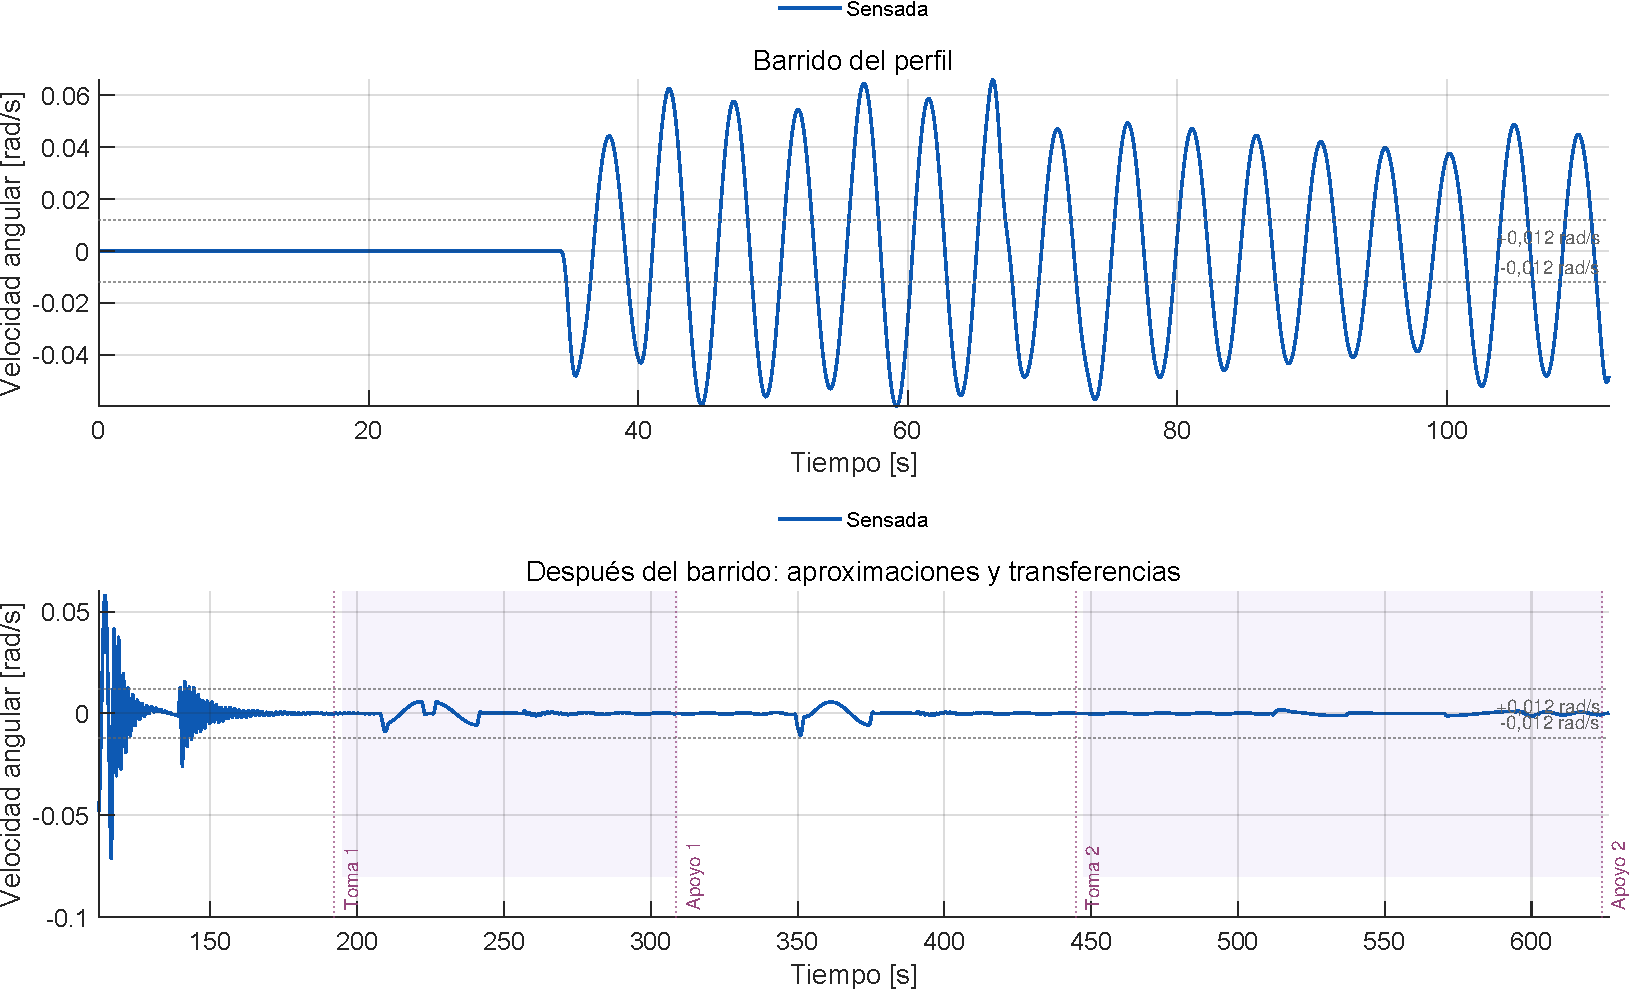
\includegraphics[width=0.98\textwidth]{imagenes_informe/prueba_completa_MIL/paneles_0810/velocidad_angular_dos_etapas.pdf}
\caption{Velocidad angular sensada durante el barrido y las maniobras posteriores. Las líneas horizontales indican los umbrales de estabilidad $\pm0.012~\mathrm{rad/s}$ para habilitar el descenso automático.}
\label{fig:completa_MIL_velocidad_angular_etapas}
\end{figure}

\par
Las contribuciones de realimentación y anticipación permiten relacionar el balanceo con la corrección aplicada. Su suma modifica el comando de velocidad del carro respecto de la referencia base.

\begin{figure}[H]
\centering
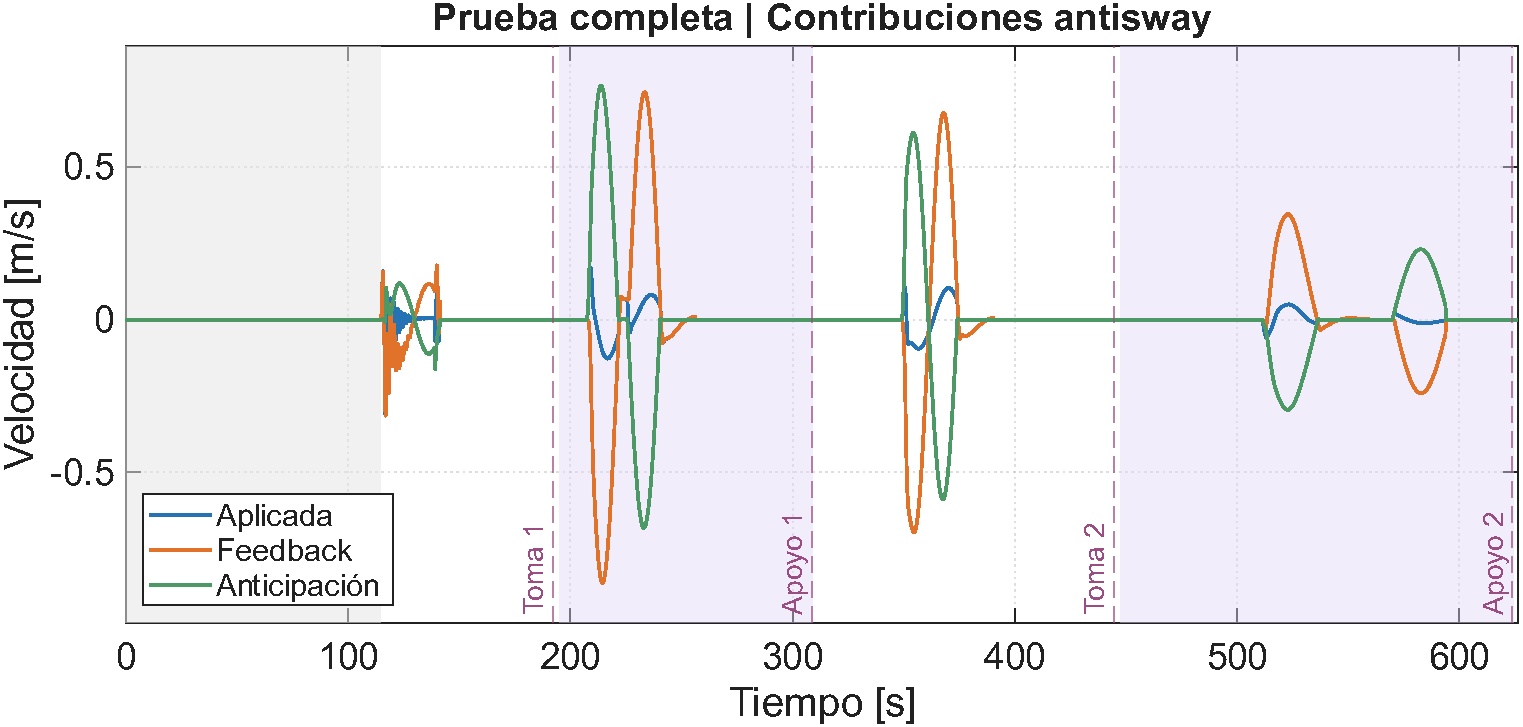
\includegraphics[width=0.98\textwidth]{imagenes_informe/prueba_completa_MIL/antisway.pdf}
\caption{Contribución antisway aplicada y sus ramas de realimentación y anticipación.}
\label{fig:completa_MIL_antisway}
\end{figure}

\begin{figure}[H]
\centering
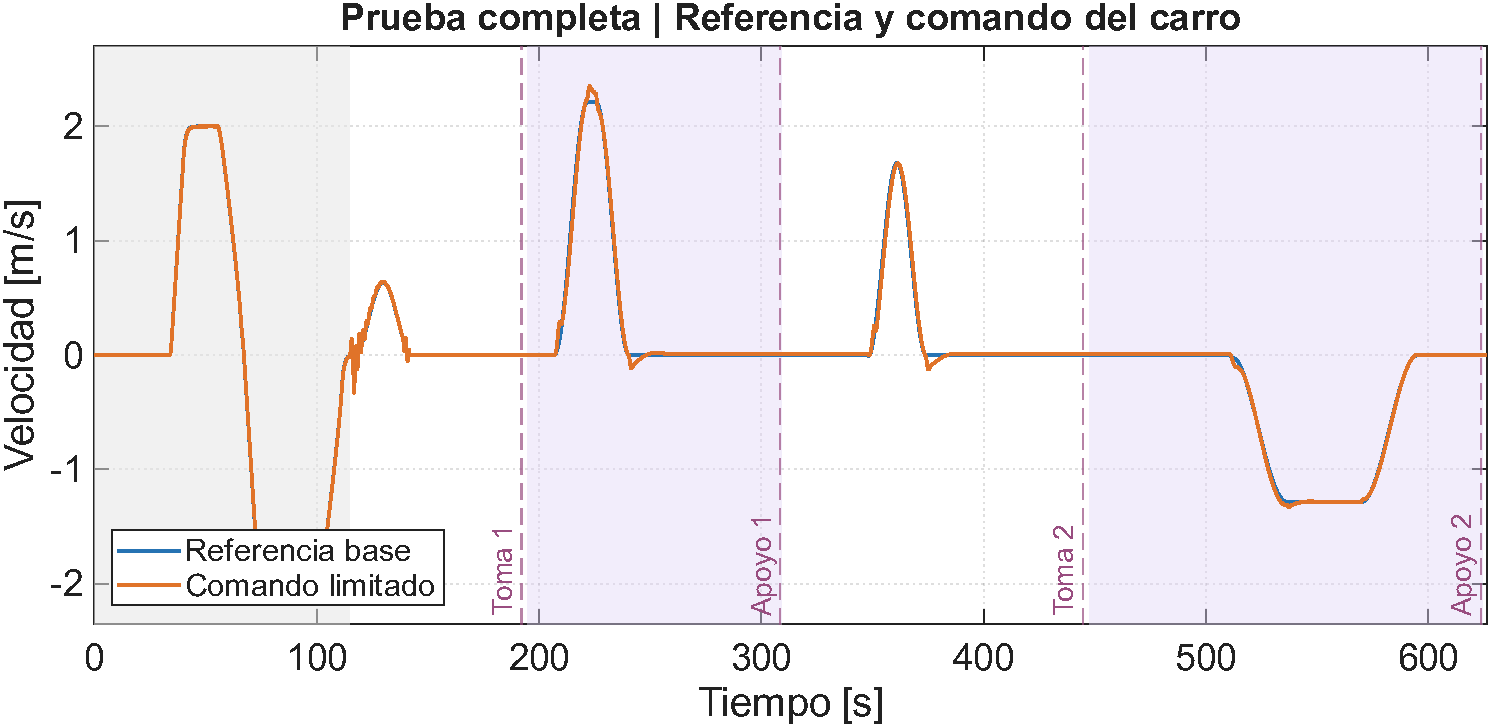
\includegraphics[width=0.98\textwidth]{imagenes_informe/prueba_completa_MIL/comando.pdf}
\caption{Referencia de velocidad base y comando del controlador del carro.}
\label{fig:completa_MIL_comando}
\end{figure}

\Needspace{8\baselineskip}
\Needspace{5\baselineskip}
\subsubsection{Torques, tensión y masa suspendida}

Para cada eje se comparan tres señales: el torque solicitado antes del limitador, el comando limitado y el torque físico del motor que actúa sobre la mecánica de la planta. Este último incluye la dinámica del accionamiento. En el carro, la señal registrada después del limitador también incorpora la autorización del eje; por tanto, una diferencia durante la parada no implica necesariamente saturación.

Las líneas horizontales indican los límites de $\pm4~\mathrm{kN\,m}$ para el carro y $\pm20~\mathrm{kN\,m}$ para el izaje. Los máximos absolutos del torque físico del motor fueron de $1.073$ y $15.294~\mathrm{kN\,m}$, respectivamente, inferiores a esos límites en esta corrida.

\begin{figure}[H]
\centering
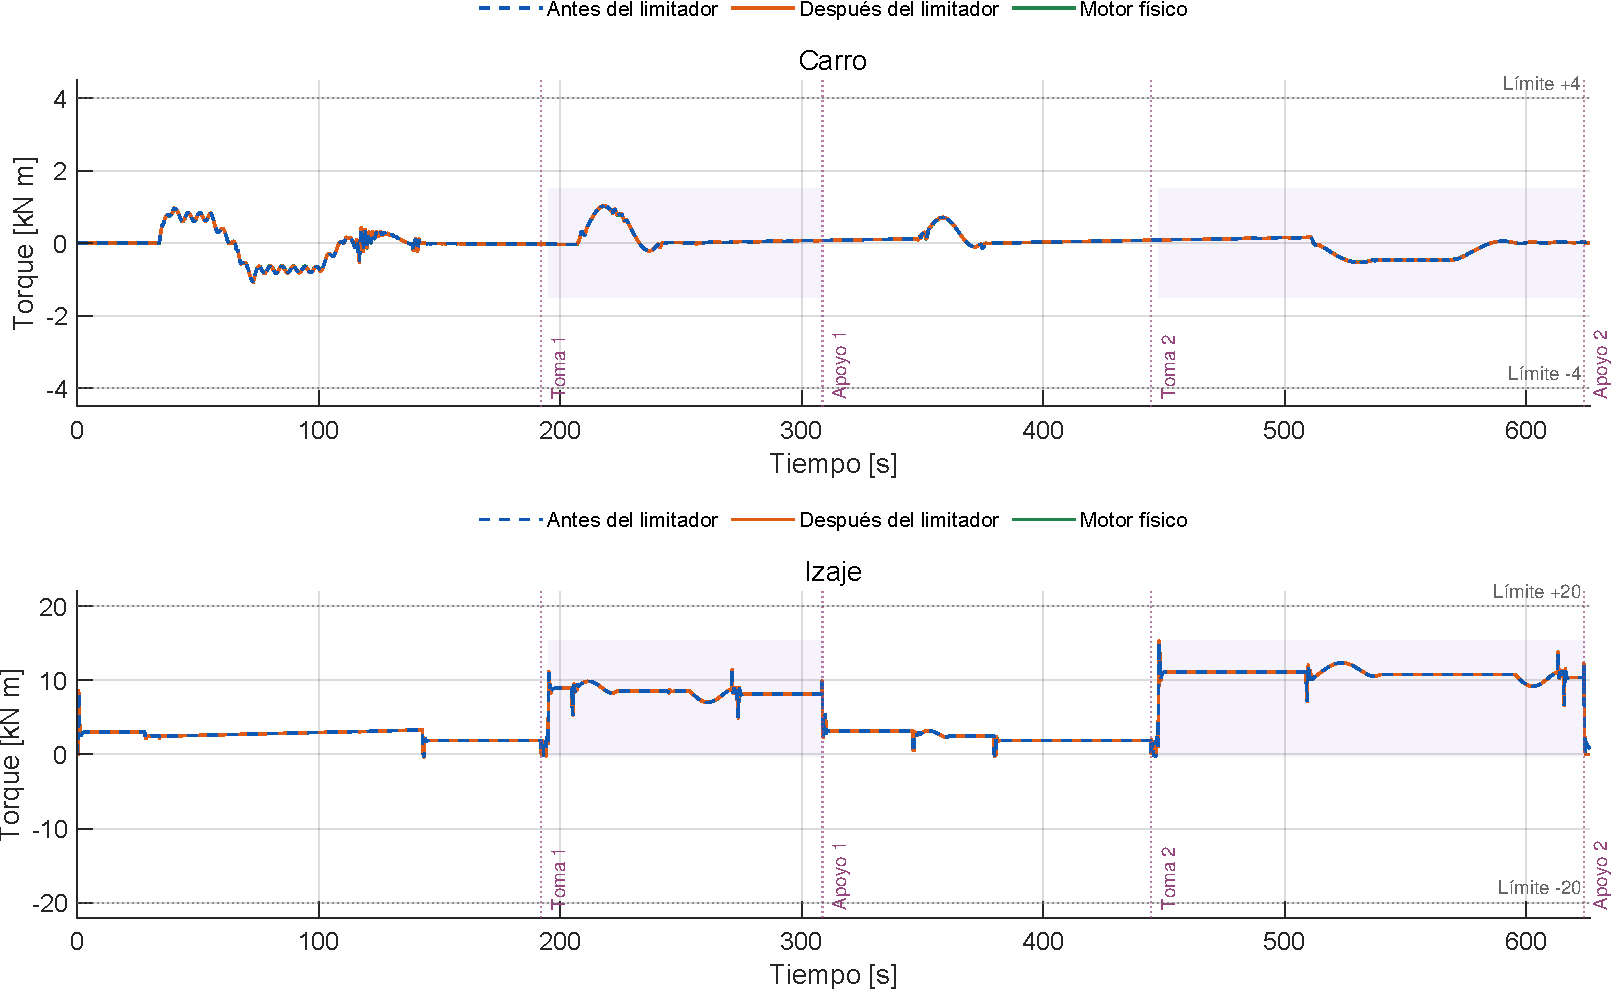
\includegraphics[width=.98\textwidth,height=.38\textheight,keepaspectratio]{imagenes_informe/prueba_completa_MIL/paneles_0810/torques_dos_ejes.pdf}
\caption{Torques del carro (arriba) y del izaje (abajo): comando antes del limitador, comando después del limitador y torque físico del motor aplicado a la mecánica.}
\label{fig:completa_MIL_torques_panel}
\end{figure}

\par
La tensión del cable complementa la identificación de las tomas y entregas. La masa física del conjunto cambia al vincular o liberar cada contenedor; se resume en el cuadro, evitando una figura adicional. Los tiempos del cuadro son los cambios de masa registrados en la planta y pueden preceder a la confirmación del operador de la cronología anterior.

\begin{table}[H]
\centering\small
\caption{Cambios de masa física del conjunto suspendido.}
\label{tab:masa_completa_MIL}
\begin{tabular}{C{.15\textwidth}L{.45\textwidth}C{.20\textwidth}}\toprule
Tiempo [s] & Estado & Masa [kg]\\\midrule
0,00 & Spreader vacío & 15\,000\\
194,95 & Primer contenedor vinculado & 50\,990\\
308,64 & Primer contenedor liberado & 15\,000\\
447,53 & Segundo contenedor vinculado & 64\,397\\
624,04 & Segundo contenedor liberado & 15\,000\\\bottomrule
\end{tabular}
\end{table}

\begin{figure}[H]
\centering
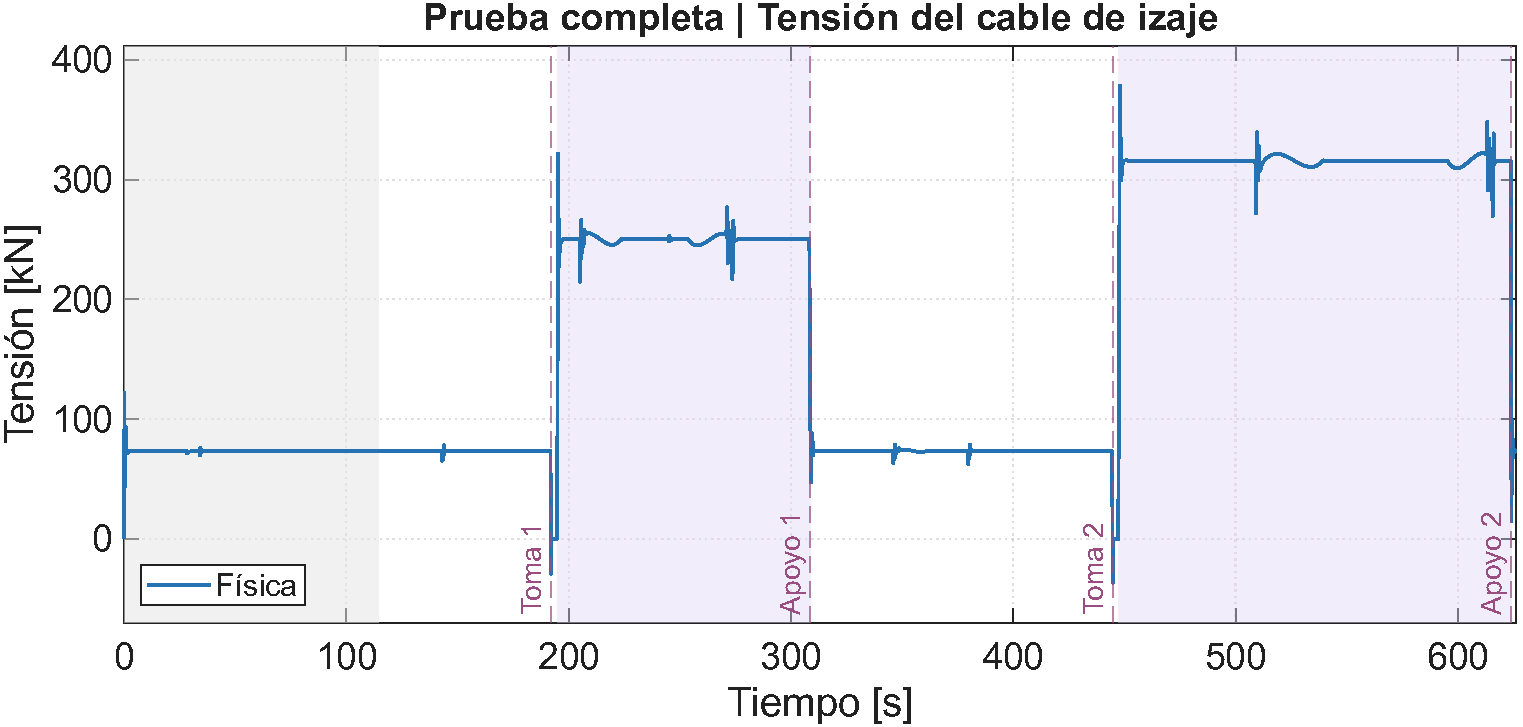
\includegraphics[width=0.98\textwidth]{imagenes_informe/prueba_completa_MIL/tension.pdf}
\caption{Tensión física del cable durante el relevamiento, las tomas y las entregas.}
\label{fig:completa_MIL_tension}
\end{figure}

\par
\Needspace{5\baselineskip}
\subsubsection{Duraciones de las transferencias y etapas vacías}

Para distinguir el tiempo de transporte cargado del tiempo de preparación, se consideran las confirmaciones registradas de toma y liberación. La primera transferencia, del muelle al barco, comprendió $114{,}04~\mathrm{s}$ desde la toma confirmada hasta la liberación. La segunda, del barco al muelle, comprendió $176{,}76~\mathrm{s}$. Estos tiempos incluyen la extracción, el traslado, el descenso y la entrega; no corresponden solamente al recorrido automático del carro.

Entre la primera liberación y la segunda toma transcurrieron $138{,}56~\mathrm{s}$. Este intervalo incluye la elevación del spreader vacío, su reposicionamiento en el barco, la aproximación y la preparación de la segunda toma. No se realizó un retorno vacío después de la segunda entrega: el ensayo finalizó con la parada.

\begin{table}[!htb]
\centering\small
\caption{Duraciones de la prueba completa MIL. Los eventos corresponden a la cronología registrada, con paso de operador de $40~\mathrm{ms}$.}
\label{tab:duraciones_completa_MIL}
\begin{tabular}{L{.44\textwidth}C{.15\textwidth}C{.15\textwidth}C{.11\textwidth}}\toprule
Etapa & Inicio [s] & Fin [s] & Duración [s]\\\midrule
Arranque hasta primera toma (incluye barrido) & 0,24 & 194,96 & 194,72\\
Primera toma confirmada hasta primera liberación & 194,96 & 309,00 & 114,04\\
Traslado automático cargado hacia el barco & 206,88 & 270,84 & 63,96\\
Etapa vacía entre primera entrega y segunda toma & 309,00 & 447,56 & 138,56\\
Segunda toma confirmada hasta segunda liberación & 447,56 & 624,32 & 176,76\\
Traslado automático cargado hacia el muelle & 510,96 & 612,88 & 101,92\\\bottomrule
\end{tabular}
\end{table}

Las dos transferencias cargadas sumaron $290{,}80~\mathrm{s}$. El intervalo desde la primera toma hasta la segunda liberación fue de $429{,}36~\mathrm{s}$, incluida la etapa vacía intermedia. Desde la solicitud de arranque hasta la segunda liberación transcurrieron $624{,}08~\mathrm{s}$; la parada normal se confirmó a los $626{,}36~\mathrm{s}$, y el registro de señales se extendió hasta $628~\mathrm{s}$. La masa suspendida final fue de $15\,000~\mathrm{kg}$, correspondiente al conjunto vacío, después de la liberación confirmada a los $624{,}32~\mathrm{s}$.

\Needspace{5\baselineskip}

\subsubsection{Resultados y alcance de la prueba}

\begin{table}[!htb]\centering

\caption{Comprobaciones de la prueba completa MIL.}\label{tab:criterios_completa_MIL}

\begin{tabular}{L{10.8cm} C{2.6cm}}\toprule Criterio & Resultado\\\midrule

Barrido real terminado antes de la primera toma & Cumple\\

Dos tomas y dos entregas físicas en los destinos previstos & Cumple\\

Balance del perfil: dos bajas y dos altas de una altura de contenedor & Cumple\\

Conjunto vacío al finalizar la segunda entrega & Cumple\\

Ausencia de emergencia, falla de seguimiento y código de falla & Cumple\\

\bottomrule\end{tabular}\end{table}









\par


% Ensayos de medio ciclo dentro de la sección final de pruebas MIL y SIL.
\Needspace{5\baselineskip}
\subsection{Pruebas de medio ciclo CODESYS}
\label{subsec:medio_ciclo_codesys}
La etapa \textit{software in the loop} (SIL) evalúa la ejecución de los autómatas en CODESYS acoplados a la planta simulada. Se comparan principalmente las implementaciones SFC manual y ST autogenerada con antisway activado. Después se evalúa el aporte del antisway mediante una prueba adicional con SFC manual y corrección desactivada.

\Needspace{5\baselineskip}

\subsubsection{Objetivo y condiciones comunes}
Se compararon los autómatas supervisor y de seguridad programados manualmente en CODESYS mediante SFC y los autómatas en texto estructurado obtenidos mediante generación automática de código para PLC de Simulink. La planta, sensores, reguladores, visualización y HMI permanecieron en Simulink, conectados al PLC por OPC UA. En adelante se denomina SFC manual a la programación realizada manualmente y ST autogenerado al código obtenido desde Simulink. Esta distinción no describe el modo de conducción: ambas ejecuciones combinan movimientos manuales y traslado automático.

Las tres pruebas presentadas comparten perfil físico, masas, ganancias, condiciones iniciales y operador. Se precargaron las 33 alturas de la escena, con perfil válido y barrido no completado. El ensayo comienza directamente con la toma en el muelle y termina al entregar el conteiner o al detenerse por el criterio establecido.

\begin{table}[!htb]\centering\small
\caption{Condiciones comunes del banco actualizado.}\label{tab:condiciones_medio_codesys}
\begin{tabular}{L{.28\textwidth}L{.58\textwidth}}\toprule
Condición & Configuración\\\midrule
Inicio y destino & $x=-26.34~\mathrm{m}$, altura $25~\mathrm{m}$, reposo; retiro del slot 2 y destino slot 22, centro $22.46~\mathrm{m}$.\\
Masa suspendida & Spreader: $15\,000~\mathrm{kg}$; contenedor: $36\,863~\mathrm{kg}$; conjunto cargado: $51\,863~\mathrm{kg}$.\\
Perfil & 33 alturas físicas; máximo inicial $18.85~\mathrm{m}$; contenedor de altura $2.59~\mathrm{m}$.\\
Control & Reguladores de carro e izaje comunes; observadores discretizados por Tustin; rampa de habilitación antisway de $2~\mathrm{s}$ y límite de variación de su término anticipativo de $0.25~\mathrm{m/s^2}$.\\\bottomrule
\end{tabular}\end{table}


\Needspace{5\baselineskip}


\subsubsection{Procedimiento y comprobación de entrega}
Luego de solicitar START, el operador realiza la aproximación y toma manual, cierra los twistlocks y selecciona el destino. Eleva hasta la altura local segura más $1~\mathrm{m}$ y solicita automático tras esperar al menos $2~\mathrm{s}$ y alcanzar $|v_y|<0.03~\mathrm{m/s}$. En destino retoma el modo manual cuando el error horizontal es menor que $0.5~\mathrm{m}$, $|v_x|<0.25~\mathrm{m/s}$ y la altura no supera la consigna automática más $0.25~\mathrm{m}$. Finalmente desciende hasta apoyo, abre los twistlocks y verifica la entrega antes de STOP.

El autómata habilita el descenso automático únicamente cuando se cumplen simultáneamente: error horizontal absoluto $\leq0.08~\mathrm{m}$, $|v_x|\leq0.06~\mathrm{m/s}$, $|\theta|\leq0.005~\mathrm{rad}$ y $|\omega|\leq0.012~\mathrm{rad/s}$. Así, la llegada horizontal no basta si persiste el balanceo. La entrega física se confirma cuando la masa suspendida queda en $15\,000~\mathrm{kg}$ y el perfil aumenta $2.59~\mathrm{m}$ en el destino, con igual disminución en el origen.

\Needspace{5\baselineskip}

\subsubsection{Comparación de las implementaciones con antisway}
\label{sec:ensayo_codesys_manual}
\label{sec:ensayo_codesys_st}
Las dos ejecuciones utilizan el mismo MC, con sincronización por tramas de tiempo simulado y vigilancia independiente del enlace. La toma, el traslado y la aproximación al destino se desarrollaron de manera semejante. Ambas implementaciones alcanzaron el apoyo y permitieron actuar sobre los twistlocks. Las gráficas permiten evaluar el seguimiento de referencias, la amortiguación del balanceo y el esfuerzo de los accionamientos.

\begin{table}[H]\centering\small
	\caption{Eventos registrados en las ejecuciones con antisway, hasta el apoyo en destino.}
	\label{tab:eventos_con_sw_0810}
	\begin{tabular}{L{.44\textwidth}C{.18\textwidth}C{.18\textwidth}}\toprule
		Evento & SFC manual [s] & ST autogenerado [s]\\\midrule
		Solicitud START & 3,24 & 3,24\\
		Toma cargada confirmada & 49,56 & 49,52\\
		Despegue físico & 50,04 & 50,00\\
		Entrada a automático & 75,44 & 75,40\\
		Llegada horizontal & 105,84 & 105,76\\
		Entrada a manual en destino & 133,32 & 133,56\\
		Apoyo en destino & 168,92 & 169,24\\\bottomrule
\end{tabular}\end{table}

\paragraph{Seguimiento del movimiento}
Se conservan los tiempos originales: no se desplazan las curvas para hacer coincidir los eventos. El SFC manual se representa hasta su parada, a $169.20~\mathrm{s}$, y el ST hasta el apoyo, a $169.24~\mathrm{s}$. Cada implementación mantiene su propia referencia, dibujada con línea discontinua del mismo color. En buena parte del recorrido las curvas se superponen por la semejanza de ambas ejecuciones.

\begin{figure}[H]\centering
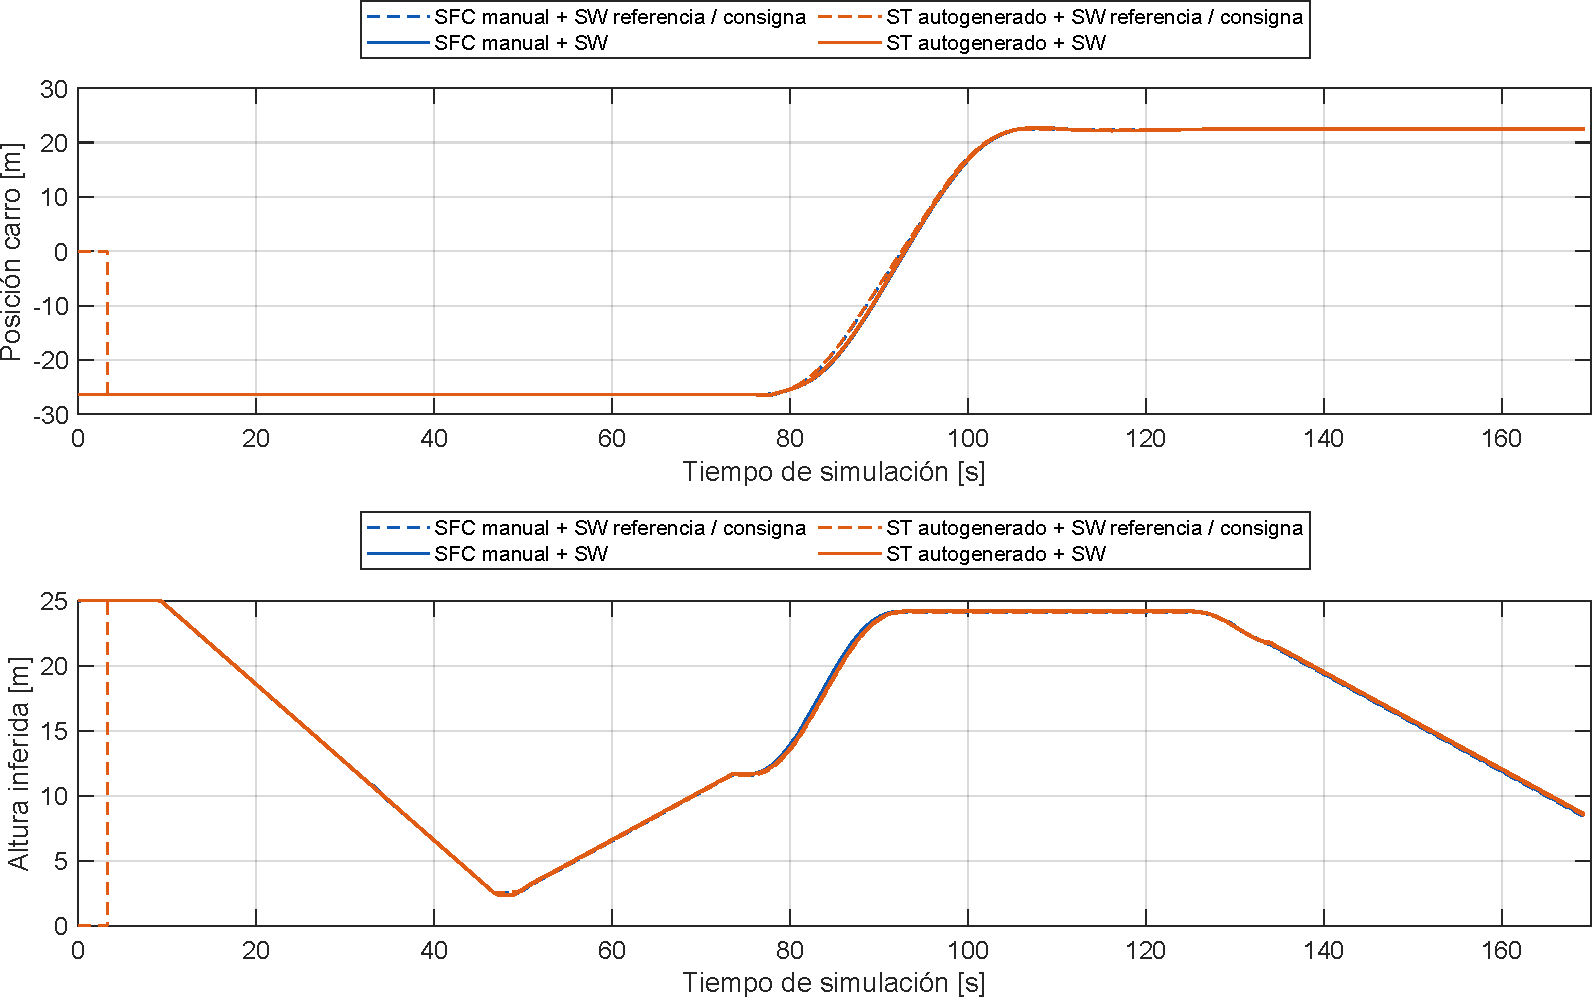
\includegraphics[width=.98\textwidth]{imagenes_informe/medio_ciclo_0810/posiciones.pdf}
\caption{Comparación con antisway: posiciones reconstruidas del carro y del izaje, junto con sus referencias. Línea continua: realimentación; discontinua: referencia.}
\label{fig:medio0810_posiciones}
\end{figure}

\par

\begin{figure}[H]\centering
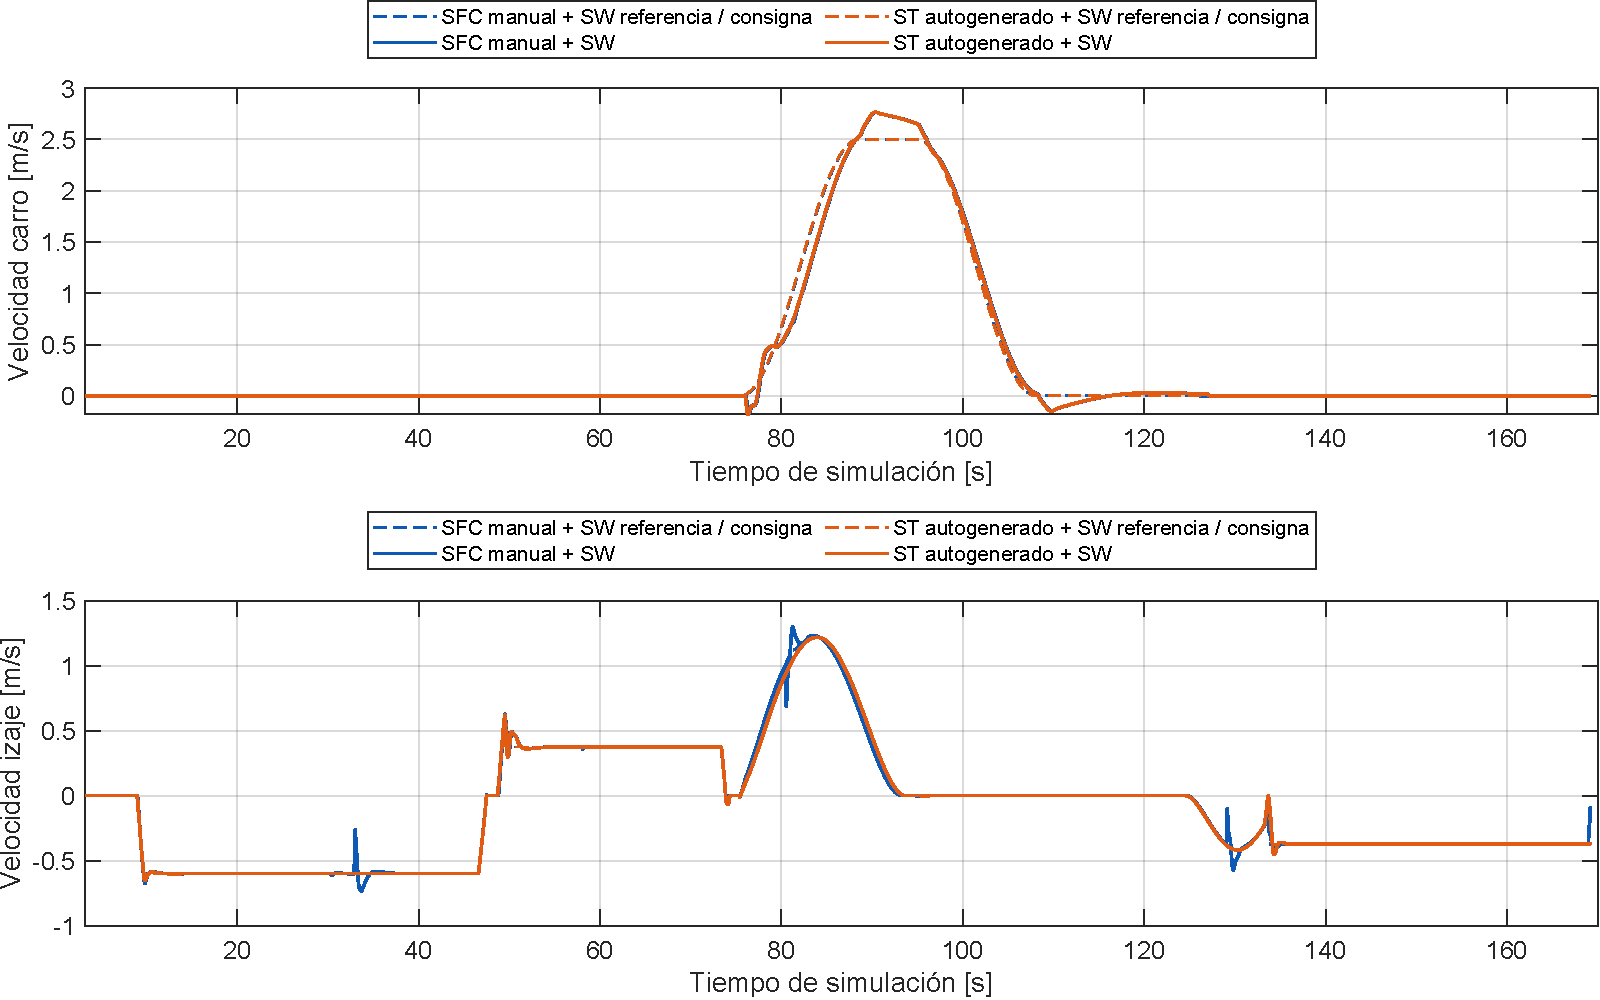
\includegraphics[width=.98\textwidth]{imagenes_informe/medio_ciclo_0810/velocidades.pdf}
\caption{Comparación con antisway: velocidades reconstruidas de carro e izaje frente a sus referencias.}
\label{fig:medio0810_velocidades}
\end{figure}


\begin{figure}[H]\centering
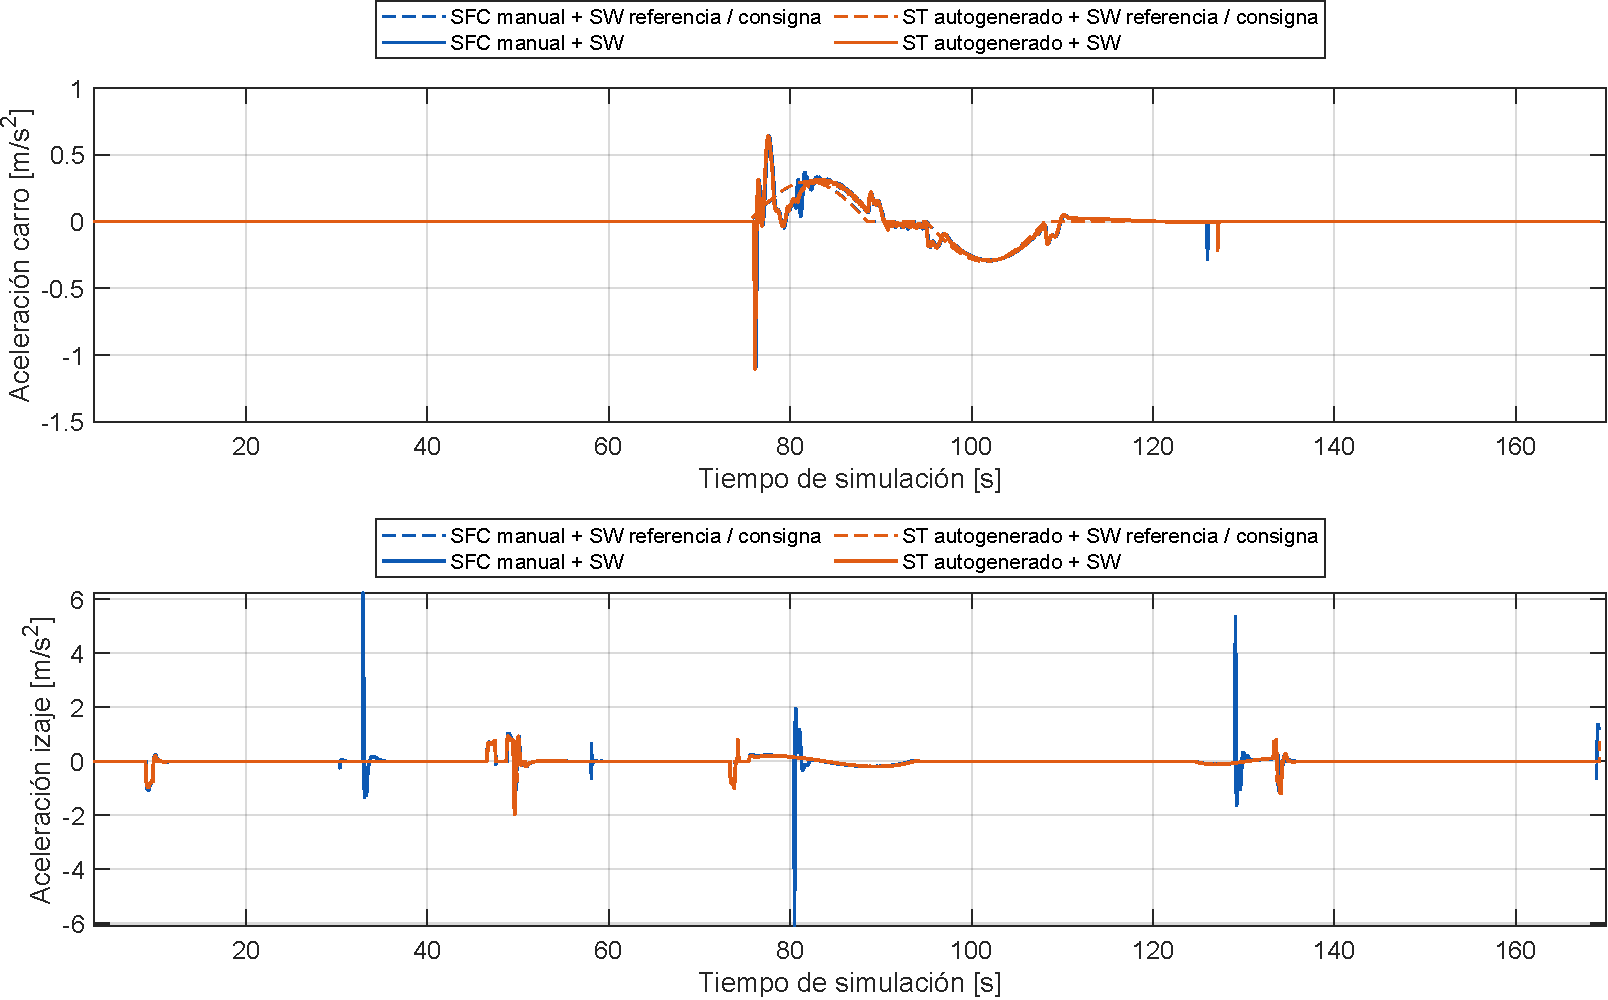
\includegraphics[width=.98\textwidth]{imagenes_informe/medio_ciclo_0810/aceleraciones.pdf}
\caption{Comparación con antisway: aceleraciones reconstruidas de los accionamientos frente a las referencias.}
\label{fig:medio0810_aceleraciones}
\end{figure}

\noindent\textbf{Balanceo y corrección aplicada}\par

\begin{figure}[H]\centering
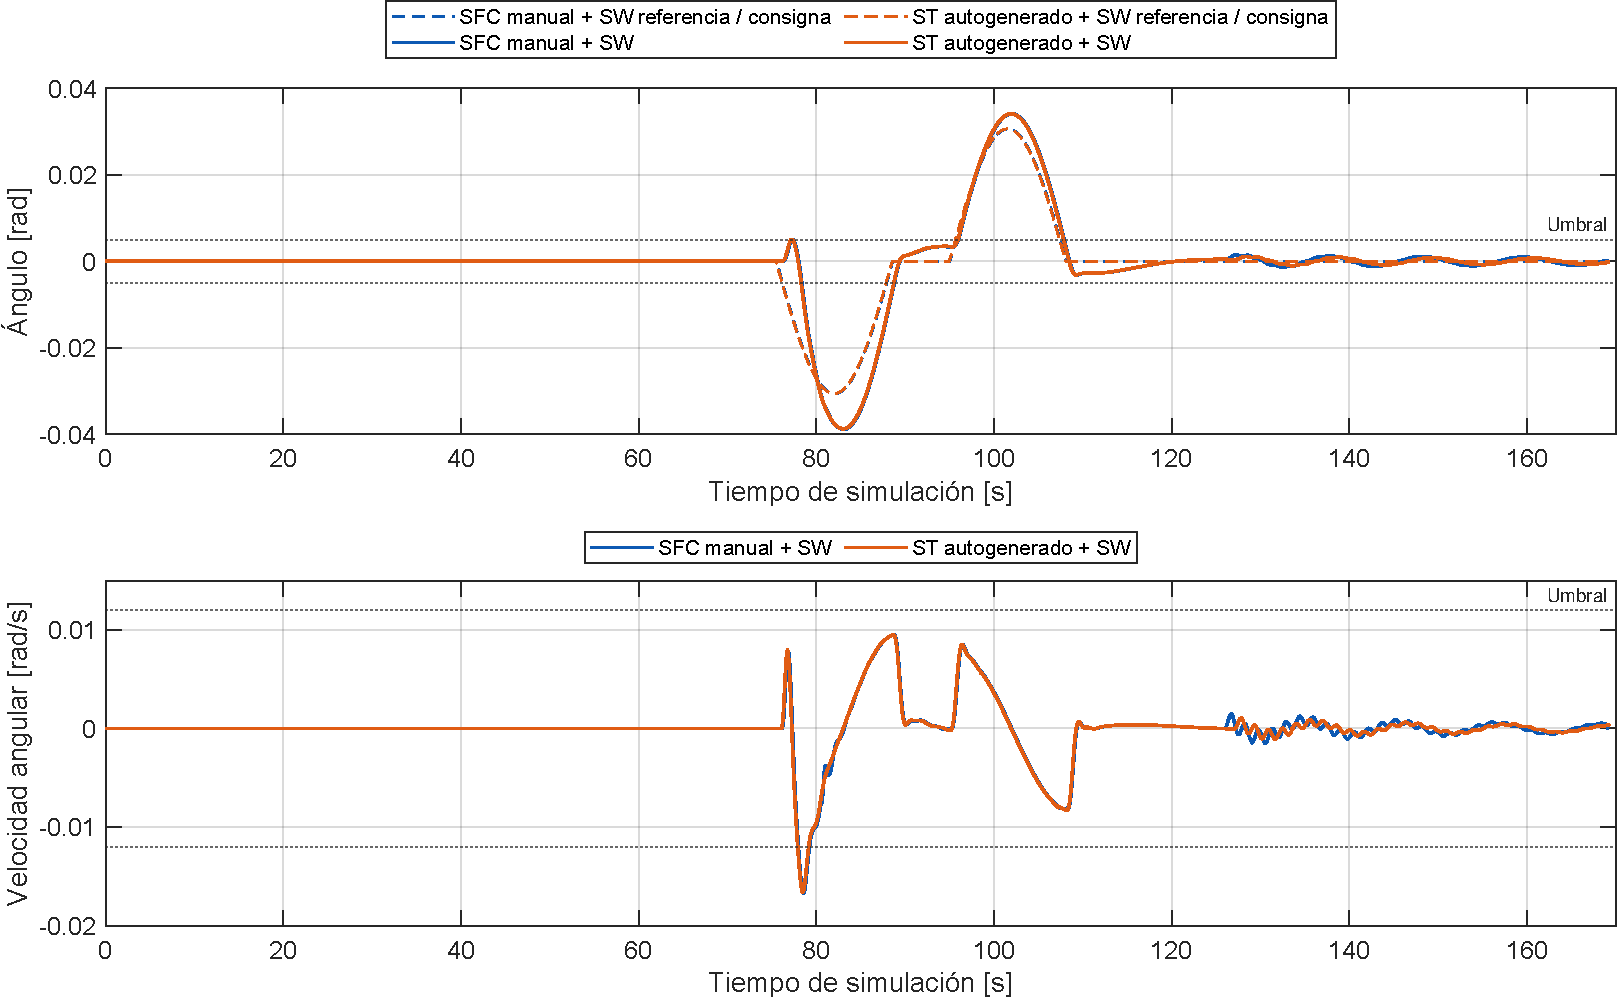
\includegraphics[width=.98\textwidth]{imagenes_informe/medio_ciclo_0810/balanceo.pdf}
\caption{Ángulo y velocidad angular de realimentación en las dos ejecuciones con antisway. El ángulo se muestra junto con su referencia; la velocidad angular se compara únicamente con los umbrales de estabilidad $\pm0.012~\mathrm{rad/s}$ del supervisor.}
\label{fig:medio0810_balanceo}
\end{figure}


\begin{figure}[H]\centering
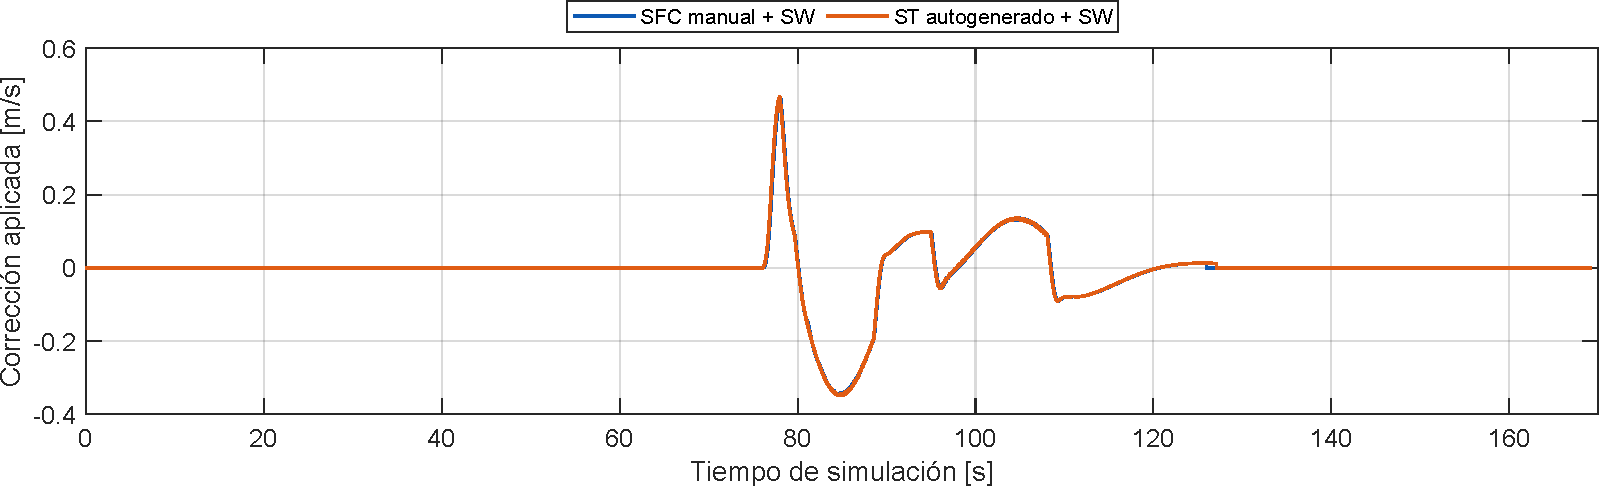
\includegraphics[width=.98\textwidth]{imagenes_informe/medio_ciclo_0810/accion_antisway.pdf}
\caption{Corrección antisway aplicada en las ejecuciones SFC manual y ST autogenerada.}
\label{fig:medio0810_accion_antisway}
\end{figure}
\par

\noindent\textbf{Torques durante la maniobra}\par

\begin{figure}[H]\centering
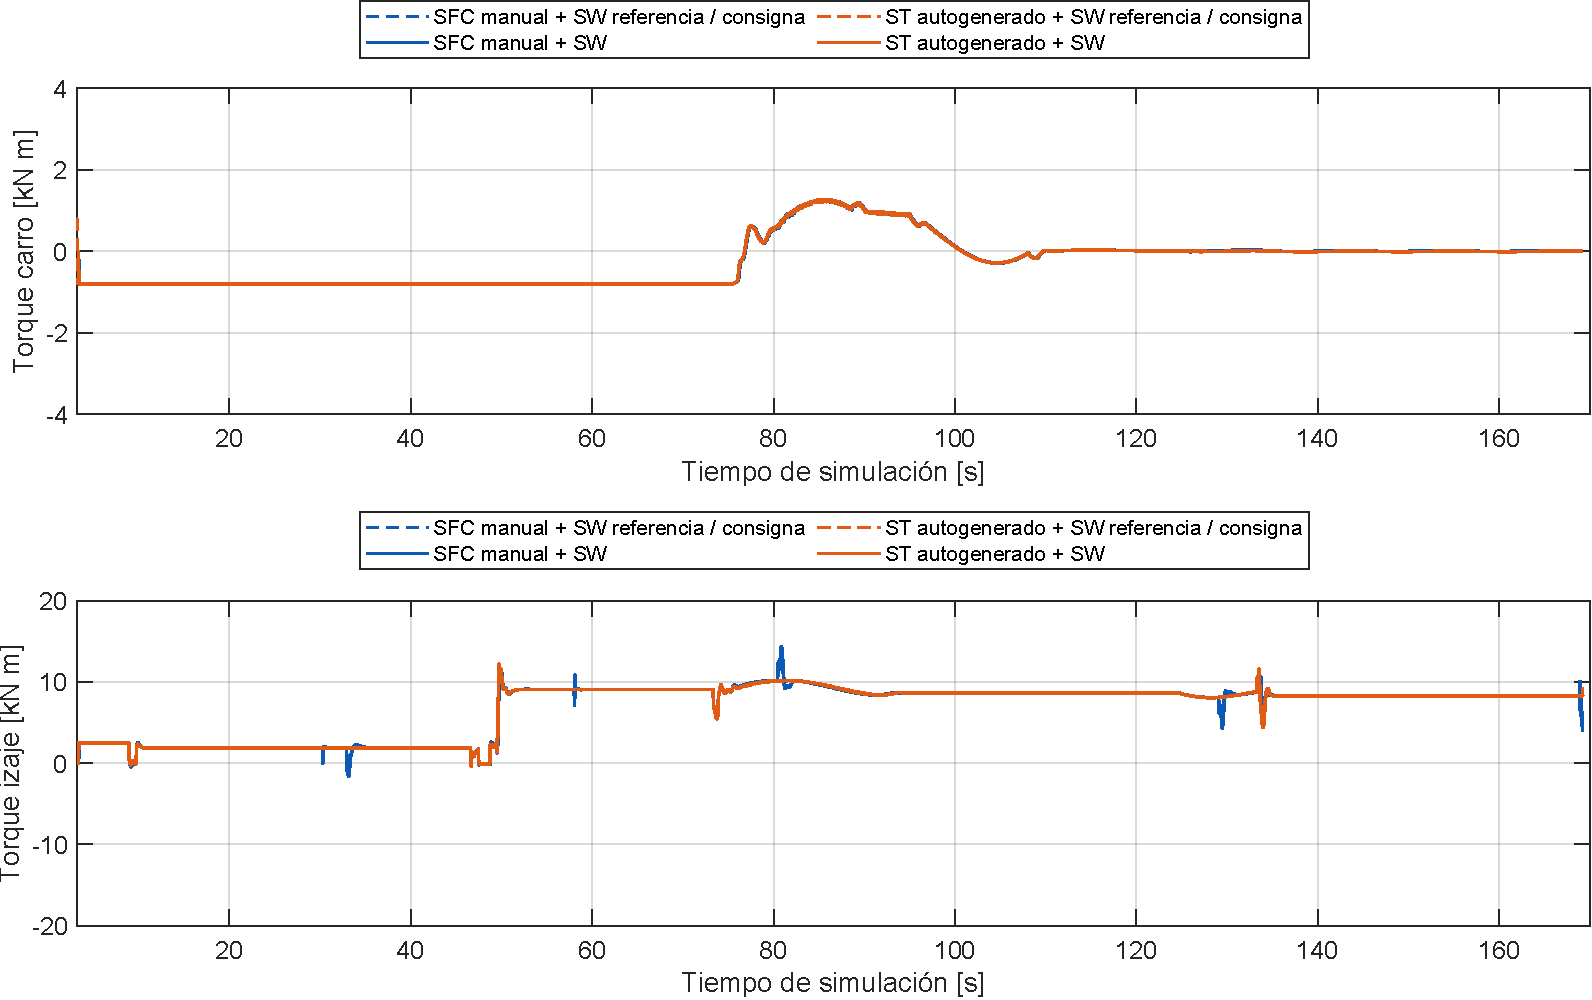
\includegraphics[width=.98\textwidth]{imagenes_informe/medio_ciclo_0810/torques.pdf}
\caption{Torques durante las maniobras con antisway, desde START hasta el apoyo o la parada. Línea continua: torque físico del motor; discontinua: consigna del controlador. Las líneas horizontales indican los límites de cada eje.}
\label{fig:medio0810_torques}
\end{figure}
\par

\Needspace{5\baselineskip}

\subsubsection{Evaluación con antisway desactivado}
Se comparó la implementación SFC manual con y sin la contribución antisway, manteniendo los demás parámetros. Sin antisway, la toma se confirmó a $49.52~\mathrm{s}$, el traslado automático comenzó a $75.44~\mathrm{s}$ y el carro llegó a la zona de destino a $105.68~\mathrm{s}$. La carga conservó un balanceo residual y permaneció a la altura de traslado durante el tramo registrado. El ensayo terminó por límite de tiempo a $187.20~\mathrm{s}$, con el contenedor suspendido, sin apoyo ni entrega.

\begin{figure}[H]\centering
	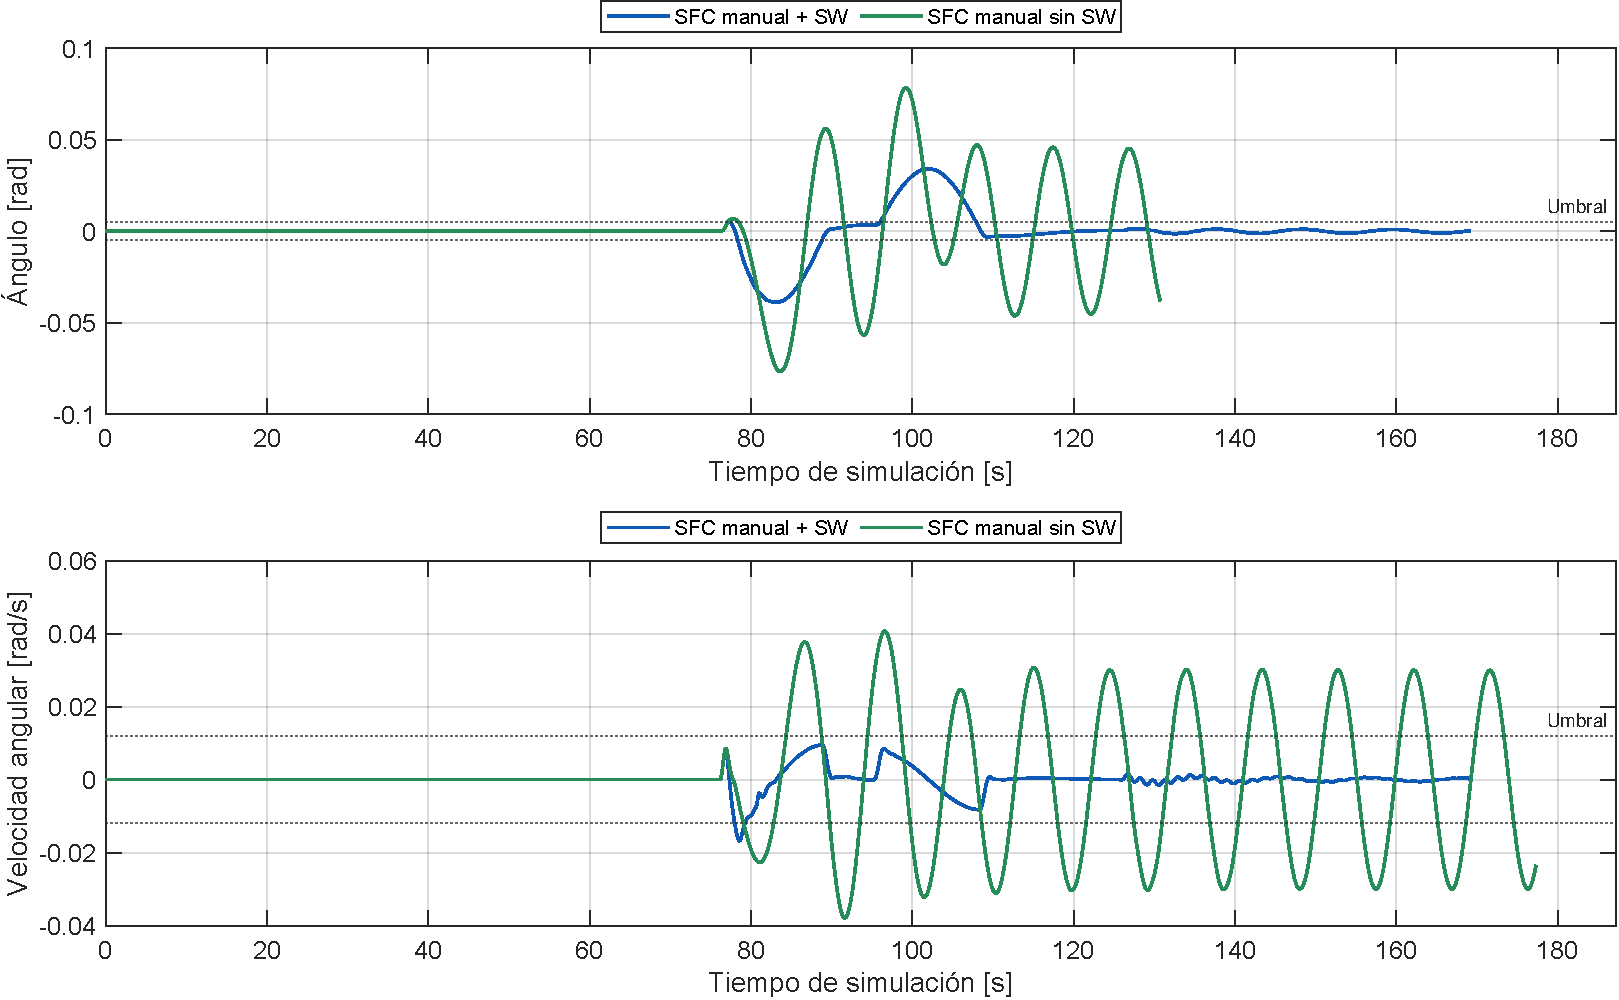
\includegraphics[width=.98\textwidth]{imagenes_informe/medio_ciclo_0810/sin_sw_balanceo.pdf}
	\caption{SFC manual con y sin antisway: ángulo y velocidad angular de realimentación. Las líneas horizontales indican los umbrales de habilitación del descenso.}
	\label{fig:medio0810_sin_sw_balanceo}
\end{figure}

La figura muestra que, sin antisway, las oscilaciones persisten después del traslado. La tabla cuantifica esta diferencia en una ventana común cubierta por los registros de ambas pruebas.

\begin{table}[H]\centering\small
	\caption{Balanceo entre $120$ y $130.72~\mathrm{s}$, para SFC manual con y sin antisway.}
	\label{tab:balanceo_manual_0810}
	\begin{tabular}{L{.38\textwidth}C{.20\textwidth}C{.20\textwidth}}\toprule
		Magnitud & Con antisway & Sin antisway\\\midrule
		Ángulo RMS [rad] & 0,000689 & 0,031222\\
		Ángulo máximo absoluto [rad] & 0,001441 & 0,045209\\
		Velocidad angular RMS [rad/s] & 0,000576 & 0,021718\\
		Velocidad angular máxima absoluta [rad/s] & 0,001499 & 0,030301\\\bottomrule
\end{tabular}\end{table}

\begin{figure}[H]\centering
	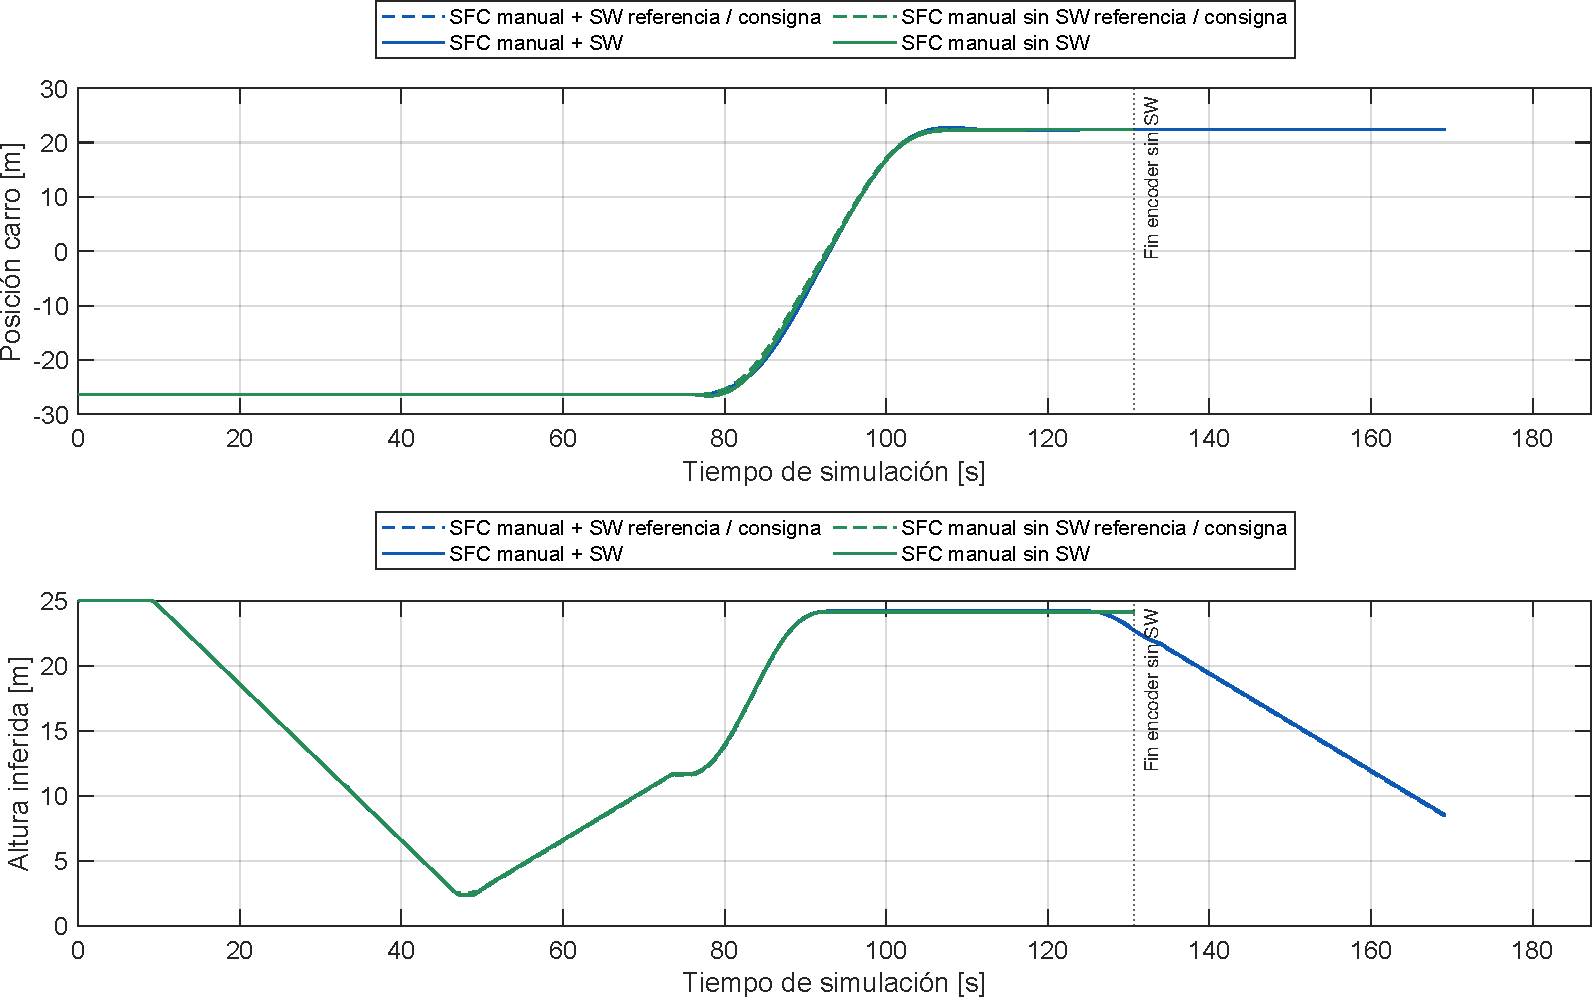
\includegraphics[width=.98\textwidth]{imagenes_informe/medio_ciclo_0810/sin_sw_posiciones.pdf}
	\caption{Posiciones reconstruidas y referencias del SFC manual con y sin antisway. La línea vertical indica el fin del registro de encoders de la prueba sin antisway.}
	\label{fig:medio0810_sin_sw_posiciones}
\end{figure}

Ambas pruebas alcanzan la zona horizontal del destino, pero sólo la ejecución con antisway continúa hacia el descenso y completa la entrega. El balanceo persistente de la otra ejecución es compatible con la espera de las condiciones de habilitación del descenso.





\par
\Needspace{5\baselineskip}
\subsection{Prueba completa con CODESYS manual}
\label{subsec:prueba_completa_codesys}
\label{subsec:prueba_integral_pendiente}
Se repite la metodología del ciclo completo MIL del apartado~\ref{subsec:prueba_completa_MIL}, ejecutando ahora los autómatas supervisor y de seguridad en CODESYS, mientras el MC, la planta, los accionamientos, los sensores y la HMI permanecen en Simulink. La maniobra comprende barrido LiDAR, dos transferencias en sentidos opuestos y parada. Se confirmaron ambas entregas físicas y la parada normal a los $611.08~\mathrm{s}$ simulados.

\Needspace{5\baselineskip}

\subsubsection{Configuración y procedimiento}
El PLC utiliza los autómatas programados manualmente mediante SFC y ST. El MC emplea la ley antisway con realimentación y anticipación separadas, limitación de la variación anticipativa y antiwindup. El intercambio OPC UA usa \texttt{Basic256Sha256} y \texttt{SignAndEncrypt}, con avance coordinado por tramas de $20~\mathrm{ms}$ simulados. El operador aplica el procedimiento ya descrito mediante los botones y el joystick de la HMI.

El ensayo comienza con el carro en $x_t=-26.34~\mathrm{m}$, altura nominal de $25~\mathrm{m}$, ejes en reposo, spreader vacío y antisway habilitado. El perfil se obtiene mediante el barrido, sin precarga. Antes de START se reconocieron una emergencia y una falla de comunicación durante la recuperación inicial del enlace; desde START, a $3.24~\mathrm{s}$, no se registraron emergencias, códigos de falla ni fallas de seguimiento.

El procedimiento conserva los mismos criterios de toma, despeje, aproximación y confirmación física que el ensayo MIL. La diferencia metodológica está en la ejecución externa de los autómatas, la sincronización y la comunicación; las duraciones de las dos corridas no se utilizan como una comparación directa de productividad.

\Needspace{5\baselineskip}

\subsubsection{Secuencia, relevamiento y transferencias}
El perfil quedó válido a los $130.08~\mathrm{s}$. La primera transferencia llevó el contenedor del slot 6, $x=-16.58~\mathrm{m}$, al slot 23, $x=24.90~\mathrm{m}$. Después se reposicionó el spreader vacío hacia el slot 32, $x=46.86~\mathrm{m}$, y se trasladó otro contenedor al slot 1, $x=-28.78~\mathrm{m}$.

\begin{table}[H]
\centering\small
\caption{Eventos de la prueba completa con CODESYS manual. Tiempos de la telemetría del operador, muestreada cada $40~\mathrm{ms}$.}
\label{tab:completa_codesys_eventos}
\begin{tabular}{L{.70\textwidth}C{.18\textwidth}}\toprule
Evento & Tiempo [s]\\\midrule
START & 3,24\\
Perfil relevado válido & 130,08\\
Contacto para la primera toma & 200,80\\
Primera toma física confirmada & 203,68\\
Primer apoyo en el barco & 315,80\\
Primera liberación confirmada & 316,24\\
Contacto para la segunda toma & 445,24\\
Segunda toma física confirmada & 448,12\\
Segundo apoyo en el muelle & 608,60\\
Segunda liberación confirmada & 609,04\\
Parada normal confirmada & 611,08\\\bottomrule
\end{tabular}
\end{table}

La entrega se verifica mediante la liberación física, la masa suspendida y el balance del perfil. Los slots 6 y 32 disminuyeron $2.59~\mathrm{m}$ y los slots 23 y 1 aumentaron esa altura. Los errores máximos del relevamiento y del balance final fueron nulos a la precisión registrada. La figura distingue los puntos LiDAR del perfil reconstruido e identifica las dos tomas y entregas.

\begin{figure}[H]\centering
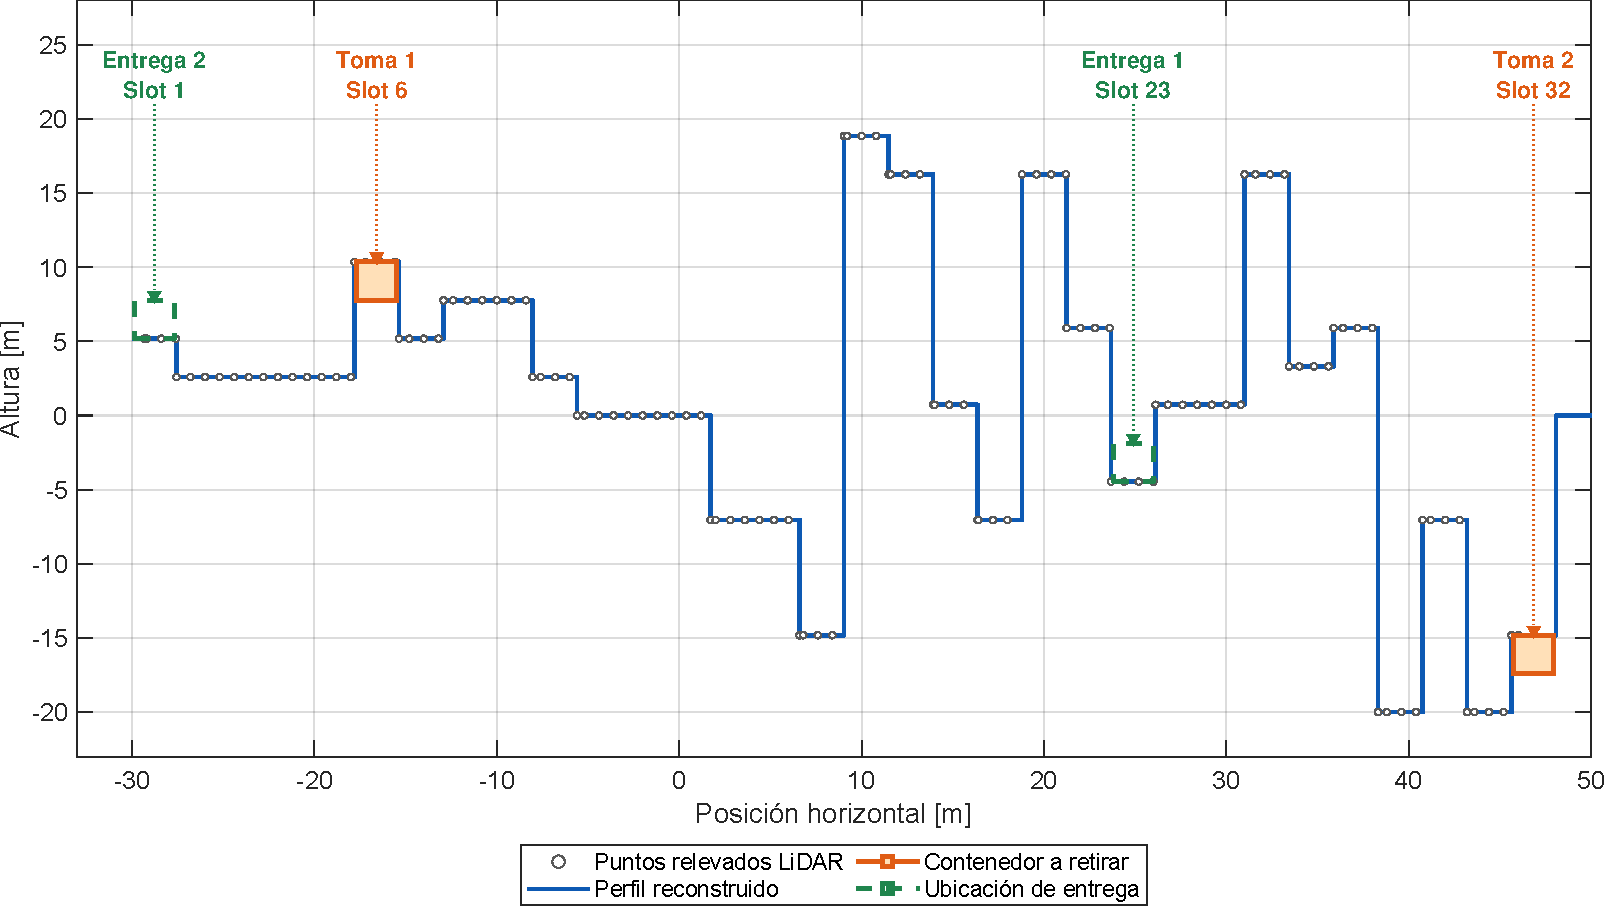
\includegraphics[width=.98\textwidth]{imagenes_informe/prueba_completa_CODESYS/perfil.pdf}
\caption{Relevamiento LiDAR y perfil reconstruido antes de las transferencias. La línea azul une las cotas de los slots mediante tramos horizontales y verticales, incluyendo las cotas neutras de los slots no operables. Se indican los contenedores a retirar y las ubicaciones de entrega: primera transferencia del slot 6 al 23 y segunda del slot 32 al 1. Las ubicaciones de entrega representan el contenedor que se añadirá sobre el perfil inicial.}\label{fig:completa_codesys_perfil}
\end{figure}

\par
\Needspace{5\baselineskip}
\subsubsection{Seguimiento del carro}
La figura reúne posición, velocidad y aceleración del carro frente a sus referencias. La posición y la velocidad se reconstruyen desde el encoder; la aceleración se calcula mediante la derivada numérica de esa velocidad, sin filtro adicional. Los paneles comienzan en START para separar la inicialización de los estimadores de la maniobra.

Como en el ciclo MIL, las franjas sombreadas delimitan las transferencias cargadas y las líneas verticales señalan los contactos de toma y apoyo. Se conservan los tiempos propios de esta corrida.

\begin{figure}[H]\centering
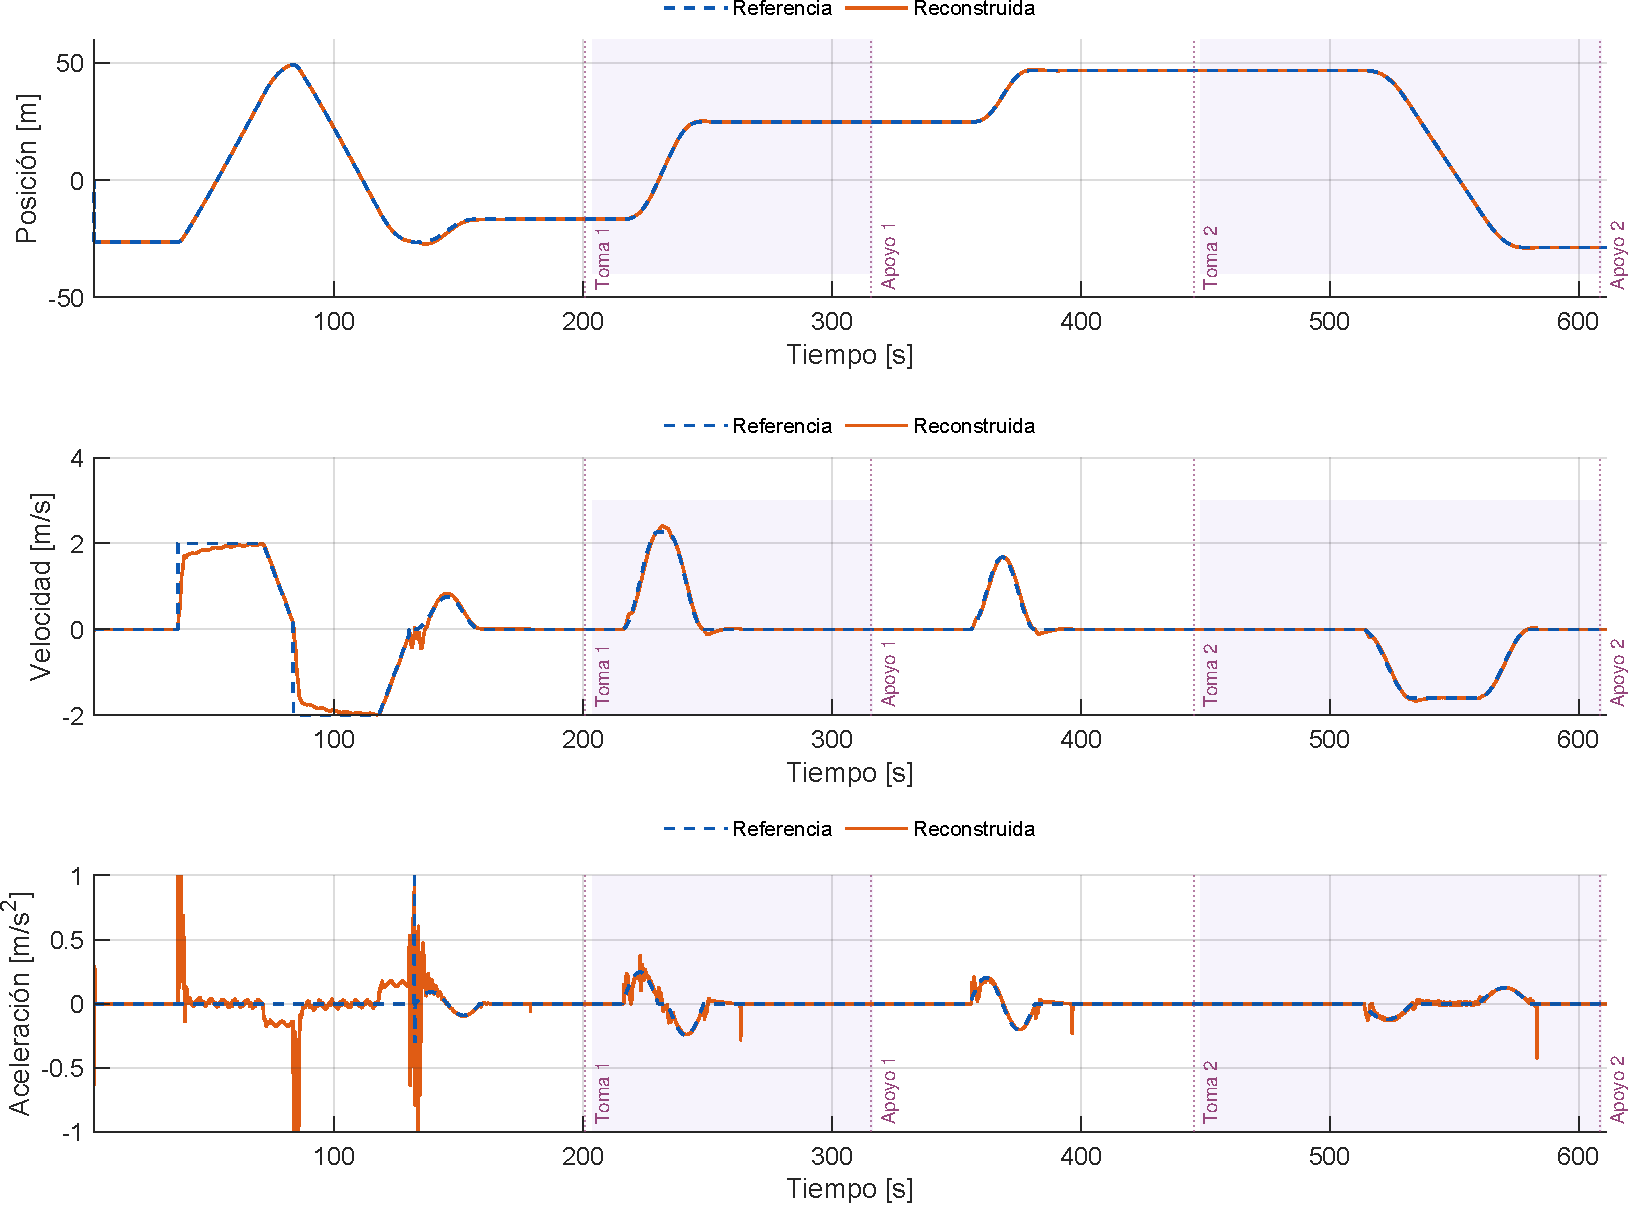
\includegraphics[width=.98\textwidth]{imagenes_informe/prueba_completa_CODESYS/paneles_0810/carro_tres_filas.pdf}
\caption{Seguimiento del carro: posición, velocidad y aceleración reconstruidas frente a sus referencias. La aceleración se representa entre $-1$ y $+1~\mathrm{m/s^2}$.}
\label{fig:completa_codesys_carro_panel}
\end{figure}


\par
\Needspace{5\baselineskip}
\subsubsection{Seguimiento del izaje y contacto}
La altura se infiere del accionamiento mediante $\widehat y_h=45~\mathrm{m}-\widehat l_h$; la velocidad es $-\dot{\widehat l}_h$ y la aceleración es su derivada numérica. Estas variables permiten observar el seguimiento del accionamiento sin superponer la altura geométrica deformada de la carga.

\begin{figure}[H]\centering
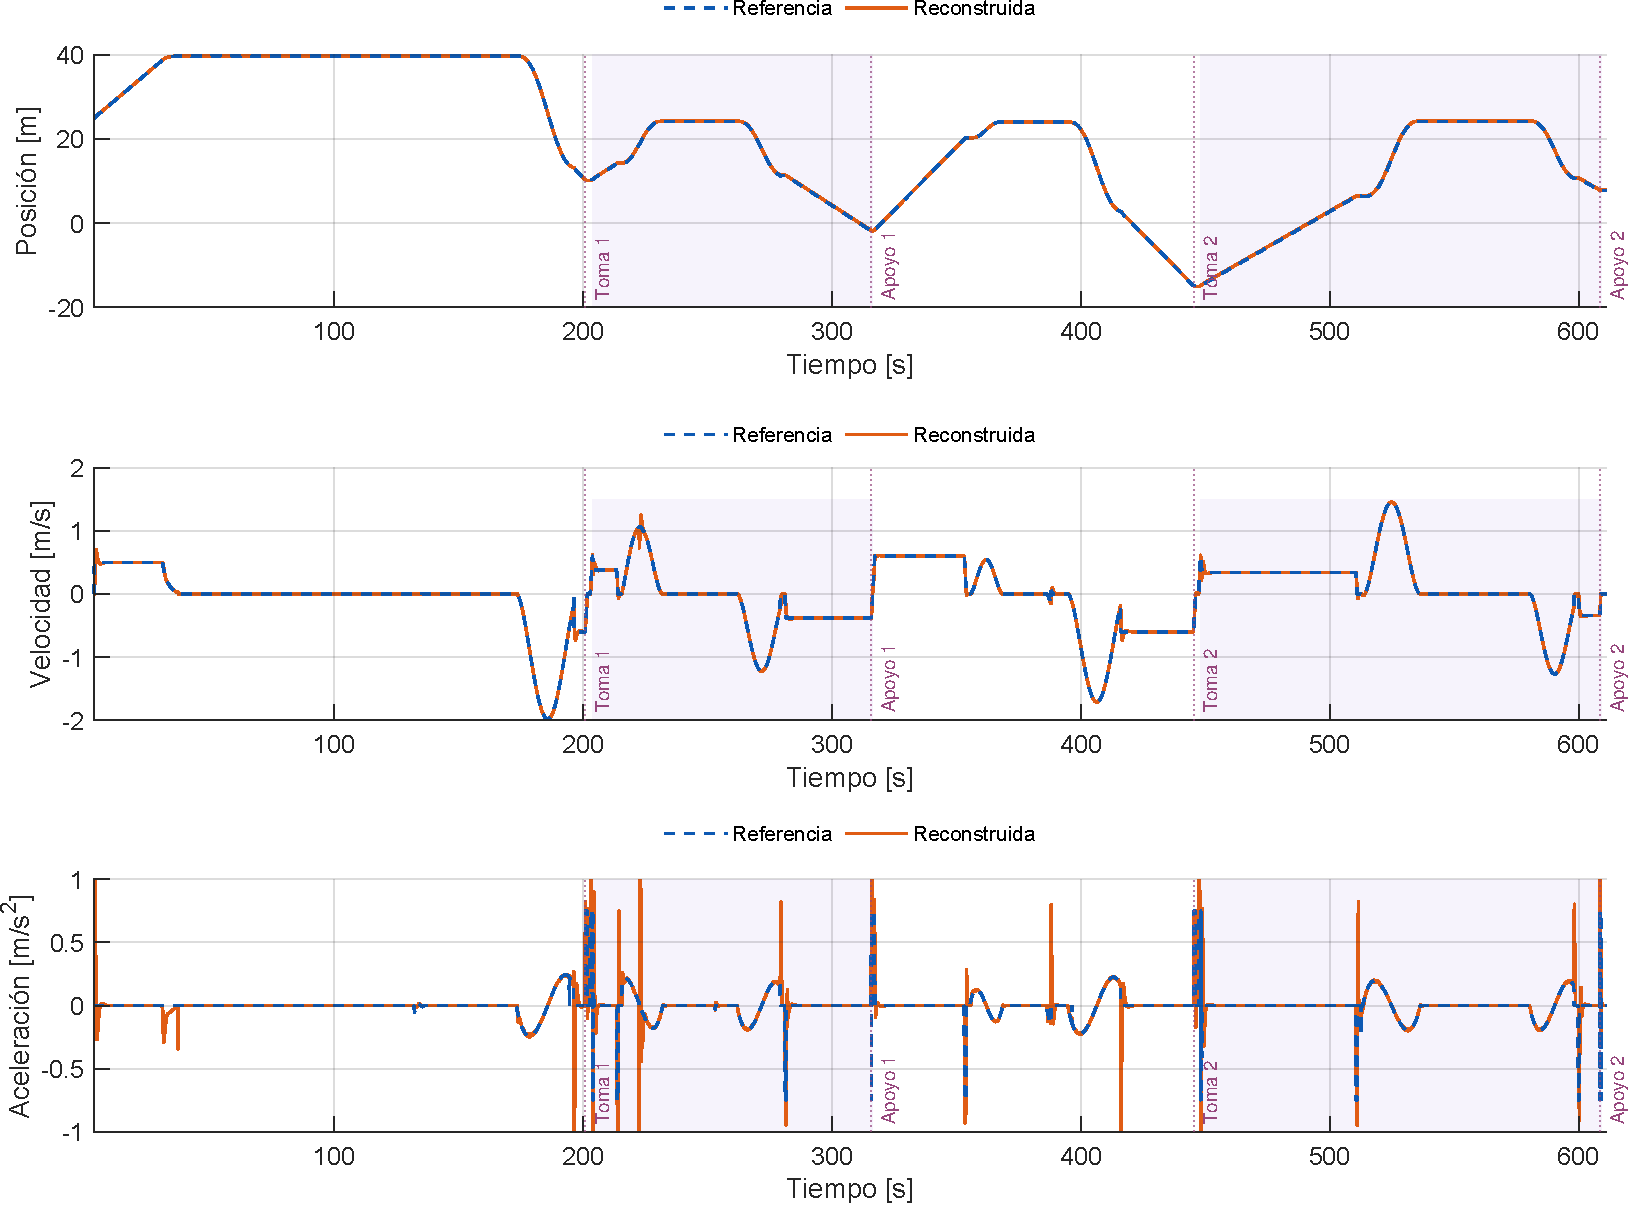
\includegraphics[width=.98\textwidth]{imagenes_informe/prueba_completa_CODESYS/paneles_0810/izaje_tres_filas.pdf}
\caption{Seguimiento del izaje: altura inferida, velocidad y aceleración reconstruidas frente a sus referencias. La escala de aceleración se recorta a $\pm1~\mathrm{m/s^2}$.}
\label{fig:completa_codesys_izaje_panel}
\end{figure}

El máximo absoluto de aceleración reconstruida fue $5.938~\mathrm{m/s^2}$, con valor negativo a $222.50~\mathrm{s}$; queda fuera del recorte vertical. Esta señal es distinta de la aceleración física de la carga, cuyo máximo fue $144.628~\mathrm{m/s^2}$ a $608.66052~\mathrm{s}$, durante el transitorio del último apoyo. El pico físico permanece en los datos guardados y no se incorpora a la escala de seguimiento del accionamiento.

\par
\Needspace{5\baselineskip}
\subsubsection{Balanceo y acción antisway}

\begin{figure}[H]\centering
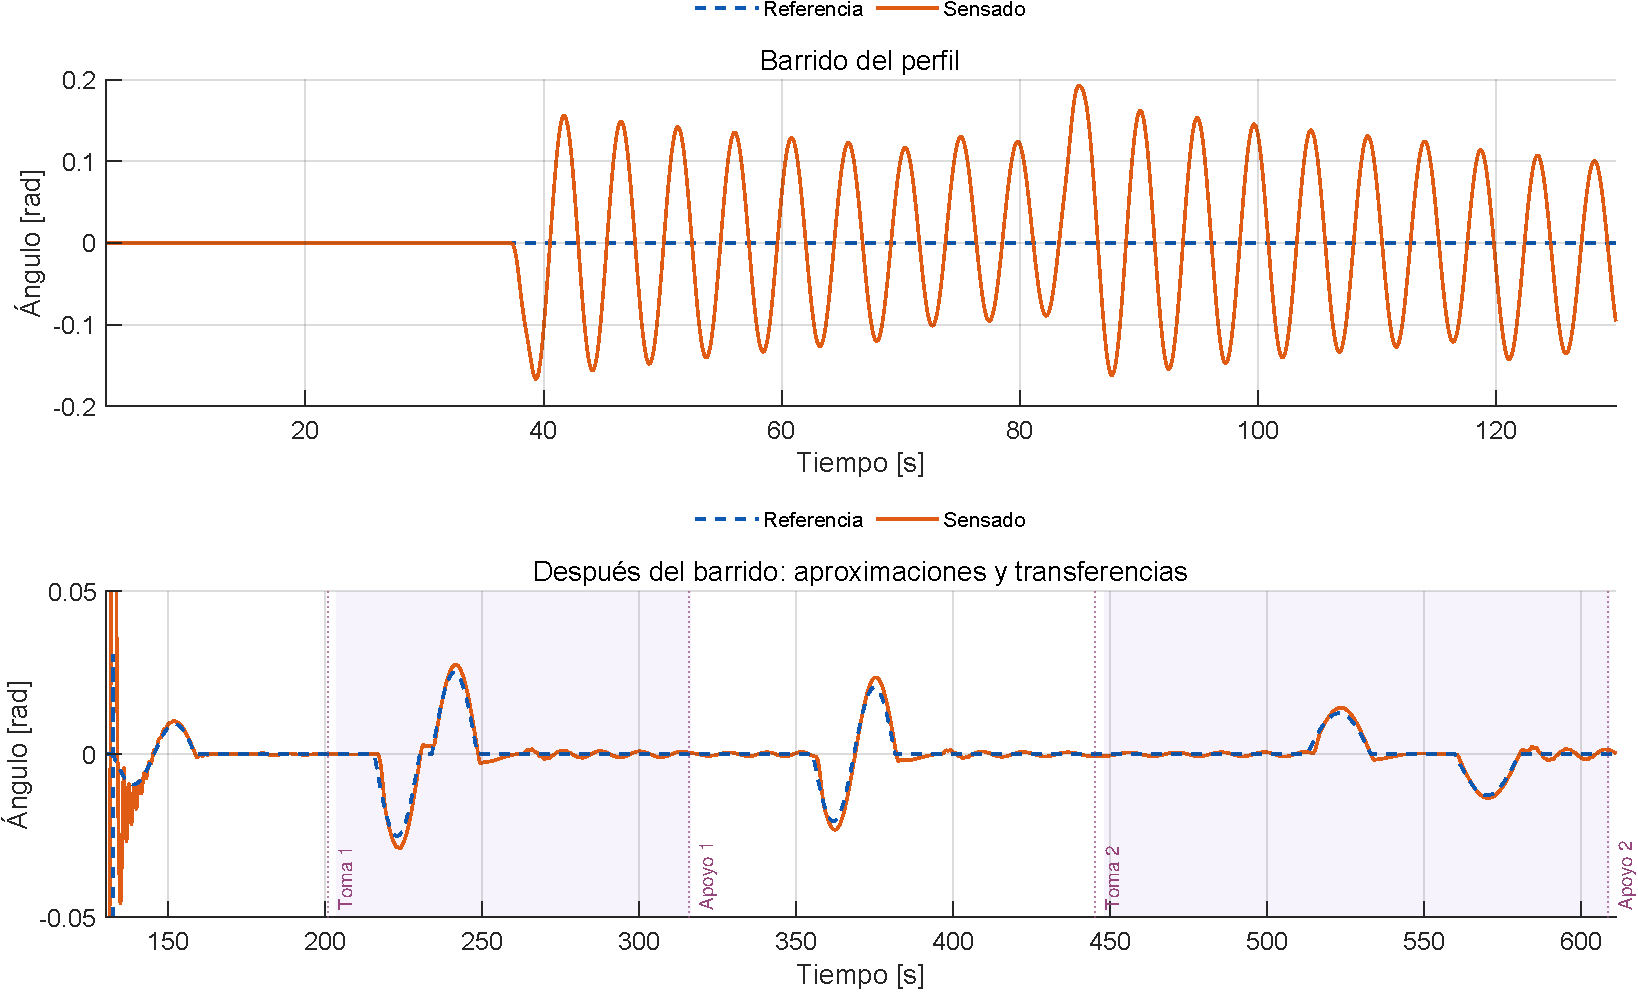
\includegraphics[width=.98\textwidth]{imagenes_informe/prueba_completa_CODESYS/paneles_0810/angulo_dos_etapas.pdf}
\caption{Ángulo de referencia y sensado durante el barrido (arriba) y las aproximaciones y transferencias posteriores (abajo).}
\label{fig:completa_codesys_angulo_etapas}
\end{figure}

Durante el primer traslado automático cargado, entre $215.56$ y $278.84~\mathrm{s}$, el máximo absoluto del ángulo fue $0.02877~\mathrm{rad}$; durante el regreso, entre $512.64$ y $597.72~\mathrm{s}$, fue $0.01425~\mathrm{rad}$. Estos valores corresponden al transporte y no a los extremos globales del barrido o de la inicialización. El transitorio posterior al barrido alcanza $|\theta|=0.12922~\mathrm{rad}$ a $130.60~\mathrm{s}$ y queda fuera de la escala de la fila inferior.

\par

\begin{figure}[H]\centering
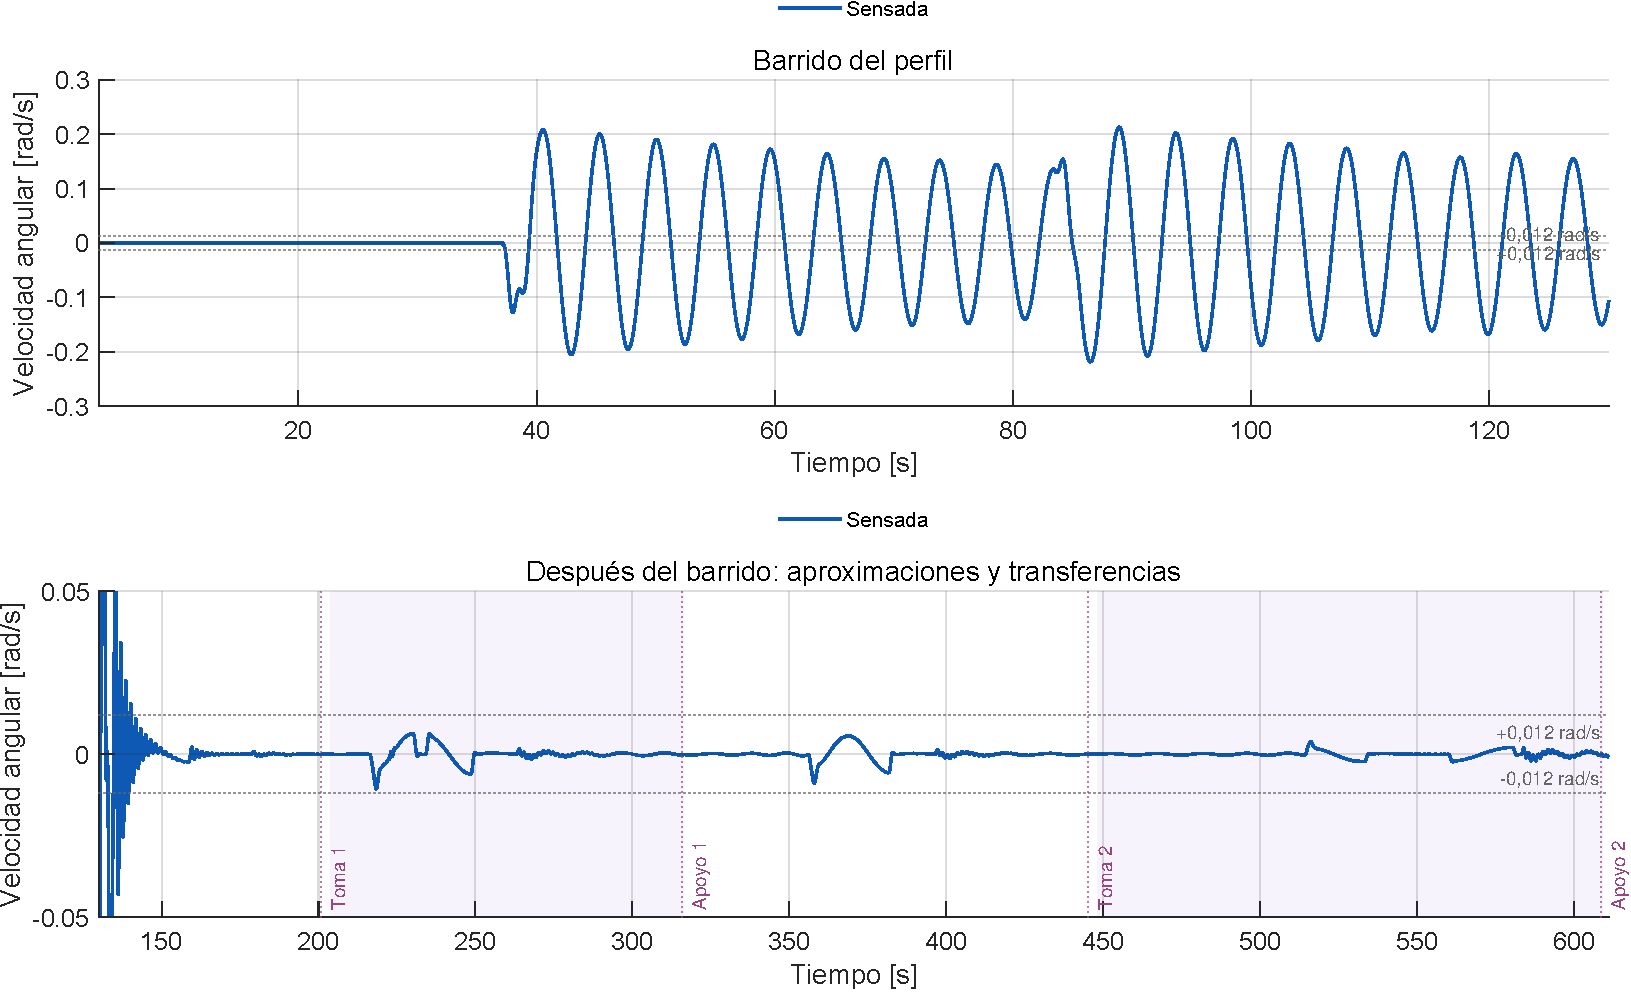
\includegraphics[width=.98\textwidth]{imagenes_informe/prueba_completa_CODESYS/paneles_0810/velocidad_angular_dos_etapas.pdf}
\caption{Velocidad angular sensada durante el barrido y las maniobras posteriores, con umbrales de estabilidad $\pm0.012~\mathrm{rad/s}$ para habilitar el descenso automático. La fila inferior conserva una escala de $\pm0.05~\mathrm{rad/s}$; los picos fuera de ella se documentan en el texto.}
\label{fig:completa_codesys_velocidad_angular_etapas}
\end{figure}

La velocidad angular sensada se compara con el umbral $|\dot\theta_l|\leq0.012~\mathrm{rad/s}$ del supervisor. Cumplirlo no basta por sí solo para habilitar el descenso: también deben verificarse las condiciones de ángulo, posición y velocidad horizontal. No se plantea un seguimiento de referencia de velocidad angular. El máximo absoluto sensado después del barrido es $0.22773~\mathrm{rad/s}$ a $131.37225~\mathrm{s}$; se documenta aquí para conservar una escala legible en el resto de la maniobra.

\begin{figure}[H]\centering
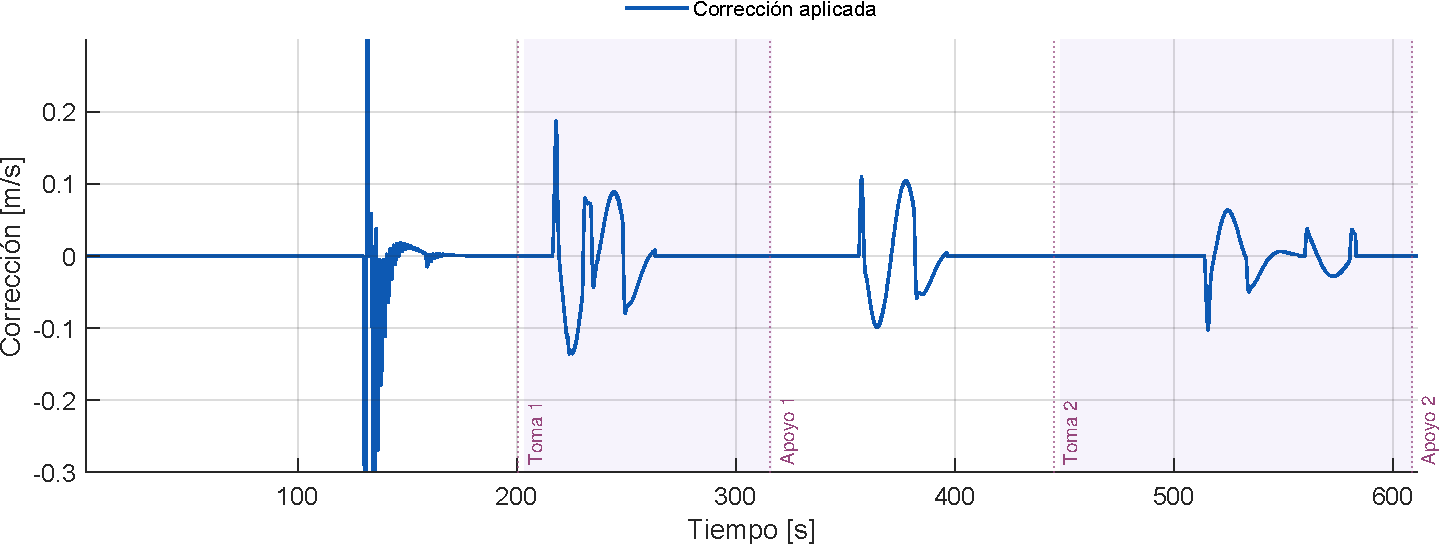
\includegraphics[width=.98\textwidth]{imagenes_informe/prueba_completa_CODESYS/paneles_0810/antisway_aplicada.pdf}
\caption{Corrección antisway efectivamente aplicada durante el ciclo completo, con escala vertical de $\pm0.3~\mathrm{m/s}$. El máximo de $1.09873~\mathrm{m/s}$ a $132.21~\mathrm{s}$ queda fuera del rango visible. El recorte es sólo gráfico y no representa un límite del controlador.}
\label{fig:completa_codesys_antisway}
\end{figure}

\par

\begin{figure}[H]\centering
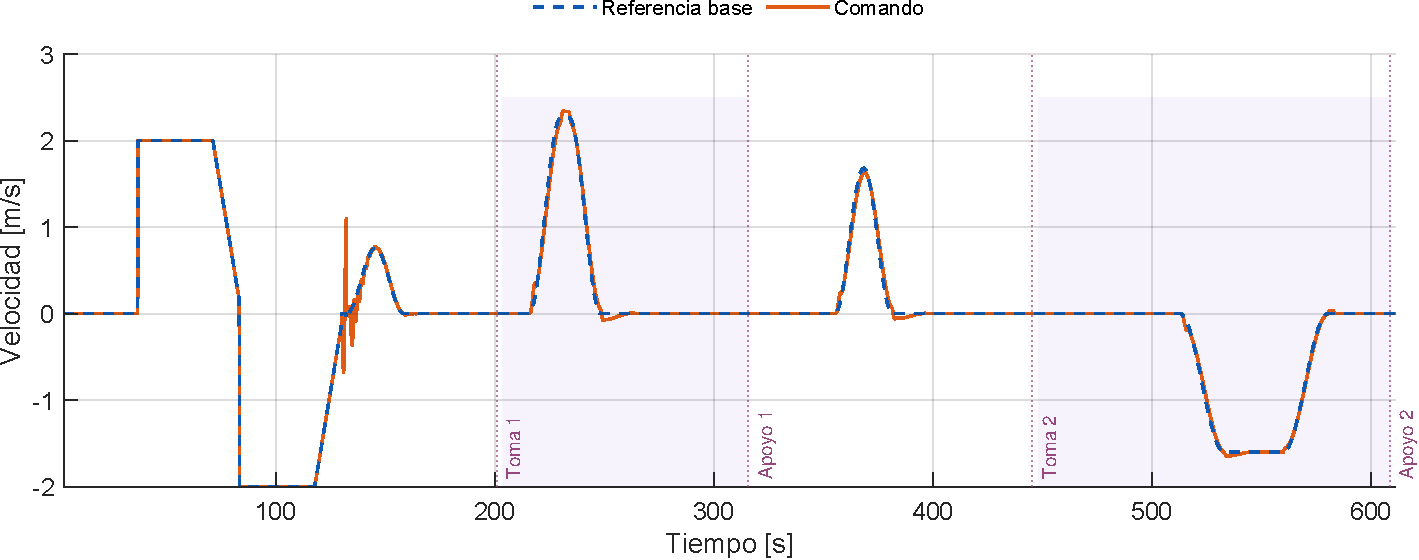
\includegraphics[width=.98\textwidth]{imagenes_informe/prueba_completa_CODESYS/paneles_0810/comando.pdf}
\caption{Referencia base de velocidad y comando del carro después de incorporar la corrección antisway.}
\label{fig:completa_codesys_comando}
\end{figure}

La diferencia entre ambas curvas muestra la intervención del antisway sobre el comando. La finalización de esta maniobra documenta el desempeño con la función habilitada; su aporte se evalúa mediante las pruebas comparables con y sin antisway del apartado de medio ciclo.

\Needspace{5\baselineskip}

\subsubsection{Torques, tensión y masa suspendida}
Se comparan tres señales por eje: comando antes del limitador, comando limitado y torque físico del motor aplicado a la mecánica. Los límites son $\pm4~\mathrm{kN\,m}$ para el carro y $\pm20~\mathrm{kN\,m}$ para el izaje. Las señales de mando también están condicionadas por los permisos de los ejes; por ello una diferencia durante la parada no implica necesariamente saturación.

\par

\begin{figure}[H]\centering
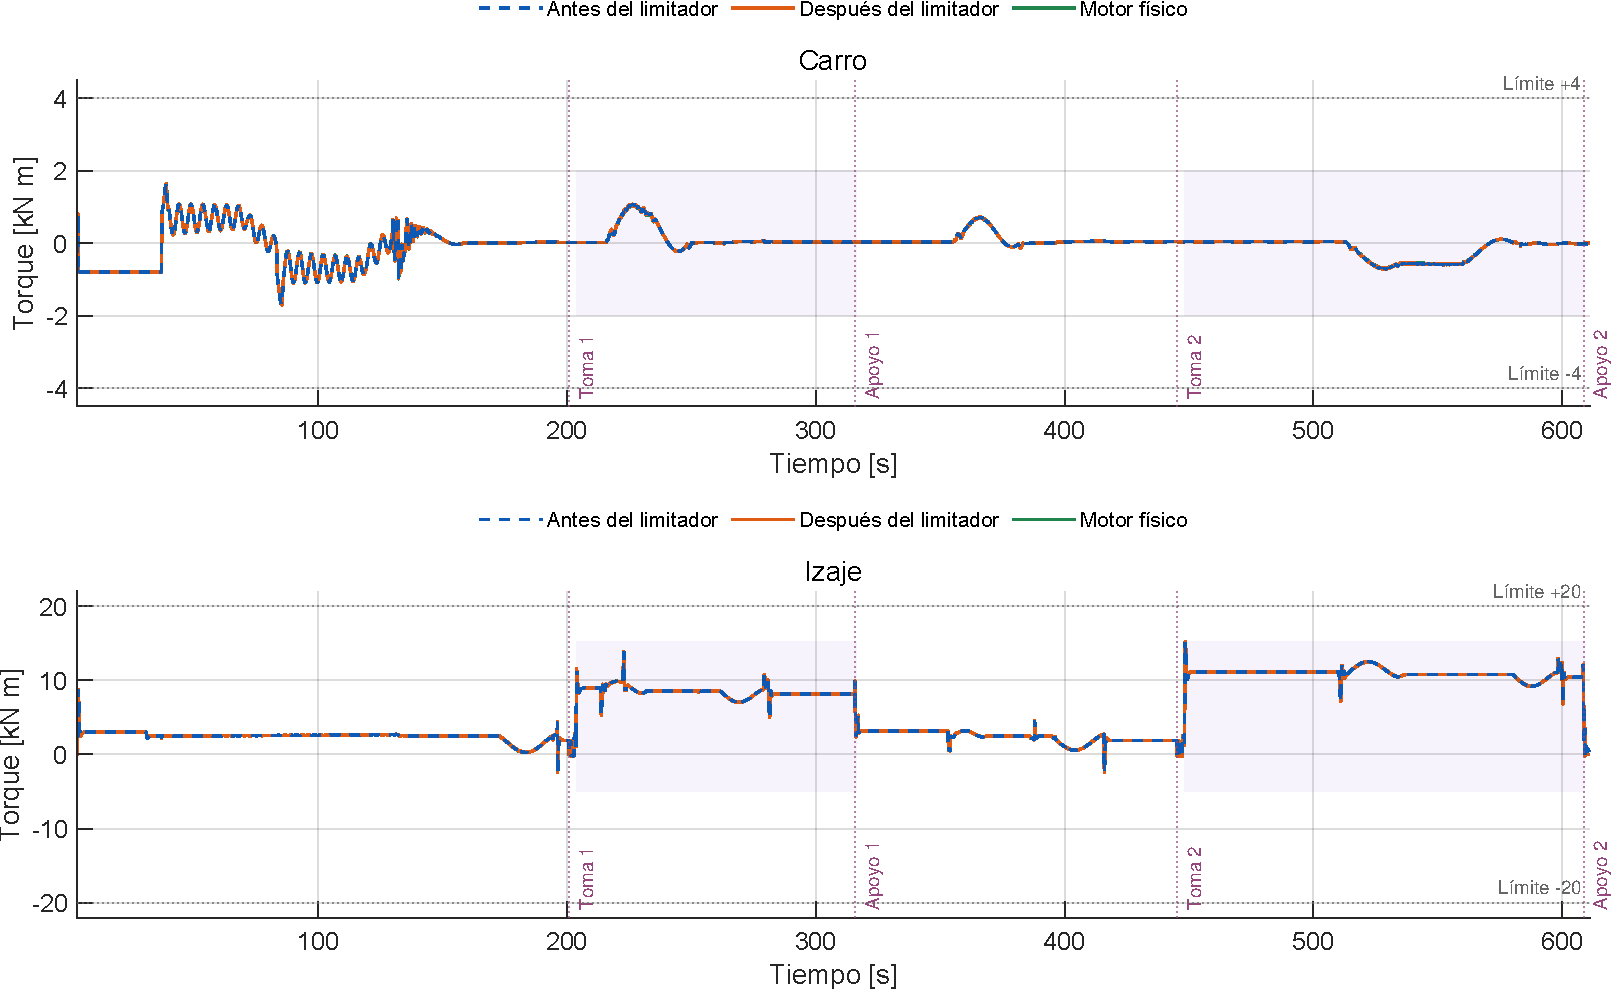
\includegraphics[width=.98\textwidth,height=.38\textheight,keepaspectratio]{imagenes_informe/prueba_completa_CODESYS/paneles_0810/torques_dos_ejes.pdf}
\caption{Torques del carro y del izaje: comando antes del limitador, comando limitado y torque físico del motor. Se muestra la maniobra desde START.}
\label{fig:completa_codesys_torques_panel}
\end{figure}

Los máximos absolutos del torque físico en el registro completo fueron $1.699$ y $15.212~\mathrm{kN\,m}$ para carro e izaje, respectivamente, inferiores a sus límites.

\par

\begin{figure}[H]\centering
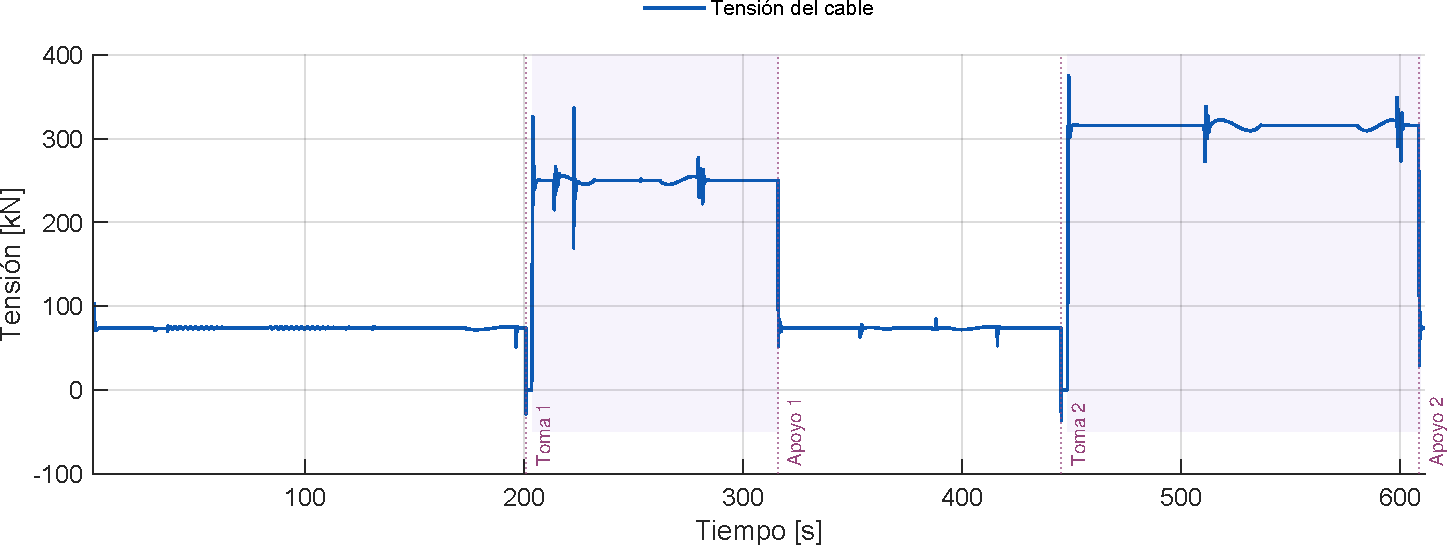
\includegraphics[width=.98\textwidth]{imagenes_informe/prueba_completa_CODESYS/paneles_0810/tension.pdf}
\caption{Tensión física del cable durante el barrido, las tomas y las entregas.}
\label{fig:completa_codesys_tension}
\end{figure}

La tensión complementa la identificación de los contactos y cambios de peso suspendido. La masa física se resume en el cuadro; sus cambios pueden preceder a las confirmaciones del operador debido a las distintas rejillas de registro.

\begin{table}[H]\centering\small
\caption{Cambios de masa física del conjunto suspendido en la prueba completa CODESYS.}
\label{tab:masa_completa_codesys}
\begin{tabular}{C{.15\textwidth}L{.45\textwidth}C{.20\textwidth}}\toprule
Tiempo [s] & Estado & Masa [kg]\\\midrule
0,00 & Spreader vacío & 15\,000\\
203,66 & Primer contenedor vinculado & 50\,990\\
315,98 & Primer contenedor liberado & 15\,000\\
448,10 & Segundo contenedor vinculado & 64\,397\\
608,66 & Segundo contenedor liberado & 15\,000\\\bottomrule
\end{tabular}\end{table}

\Needspace{5\baselineskip}

\subsubsection{Duraciones de las transferencias y etapas vacías}
Los tiempos cargados se delimitan mediante las confirmaciones de toma y entrega del operador. Incluyen extracción, traslado, descenso y liberación; los tiempos de traslado automático son una parte de ellos.

\begin{table}[H]\centering\small
\caption{Duraciones de la prueba completa con CODESYS.}
\label{tab:duraciones_completa_codesys}
\begin{tabular}{L{.44\textwidth}C{.15\textwidth}C{.15\textwidth}C{.11\textwidth}}\toprule
Etapa & Inicio [s] & Fin [s] & Duración [s]\\\midrule
Arranque hasta primera toma, incluido el barrido & 3,24 & 203,68 & 200,44\\
Primera toma confirmada hasta entrega en barco & 203,68 & 316,24 & 112,56\\
Traslado automático cargado hacia el barco & 215,56 & 278,84 & 63,28\\
Etapa vacía entre primera entrega y segunda toma & 316,24 & 448,12 & 131,88\\
Segunda toma confirmada hasta entrega en muelle & 448,12 & 609,04 & 160,92\\
Traslado automático cargado hacia el muelle & 512,64 & 597,72 & 85,08\\\bottomrule
\end{tabular}\end{table}

Las dos transferencias cargadas sumaron $273.48~\mathrm{s}$. Desde la primera toma hasta la segunda entrega transcurrieron $405.36~\mathrm{s}$, incluida la maniobra vacía intermedia. No se realizó un retorno vacío después de la segunda entrega; la parada normal se confirmó $2.04~\mathrm{s}$ después de su liberación.


\par
\Needspace{10\baselineskip}
\section{Estimación y mejora de la productividad}
\label{sec:estimacion_productividad}

\subsection{Definición del ciclo de evaluación}

El requisito de 30 contenedores por hora corresponde a un tiempo máximo de $120\un{s}$ por ciclo simple, incluyendo la transferencia cargada
y el retorno vacío. Para evaluar este requisito se ejecutó en MIL un ciclo con el Motion Controller de anticipación limitada utilizado en las pruebas anteriores.

El ensayo comienza con el spreader vacío sobre el slot 2, en
$x=-26{,}34\un{m}$ y altura nominal de $25\un{m}$, con el perfil de obstáculos conocido. La secuencia comprende el descenso, la toma del contenedor, el despegue y pesaje, el traslado al slot 22, la entrega y el retorno vacío al slot 2 a la altura de partida.
Cada traslado horizontal cubre aproximadamente $48{,}80\un{m}$.

El tiempo de ciclo se mide desde el inicio del descenso hasta la confirmación del regreso. El regreso se confirma con el conjunto vacío, error horizontal de hasta $0{,}08\un{m}$, altura $25\pm0{,}10\un{m}$, velocidades horizontal y vertical menores que $0{,}06$ y $0{,}08\un{m/s}$, respectivamente, ángulo de hasta
$0{,}5^\circ$ y velocidad angular de hasta $0{,}05\un{rad/s}$,
sostenidos durante $0{,}20\un{s}$.

La productividad estimada se obtiene como
\begin{equation}
P=\frac{3600}{T_{\mathrm{ciclo}}}\quad[\mathrm{contenedores/h}],
\qquad T_{\mathrm{ciclo}}=t_{\mathrm{fin}}-t_{\mathrm{inicio}}.
\end{equation}

\subsection{Resultado con el Motion Controller FF}

Se conservaron la regulación, el generador y los criterios operativos de la configuración FF. El operador aplicó mandos de joystick y esperas de $2\un{s}$ antes de solicitar AUTO.
La preparación del ensayo fijó la posición inicial, el perfil conocido y el objetivo de retorno a $25\un{m}$.

El tiempo de ciclo y la productividad resultaron
\begin{equation}
T_0=219{,}92-2{,}00=217{,}92\un{s},\qquad
P_0=\frac{3600}{217{,}92}=16{,}52\un{contenedores/h}.
\end{equation}

\begin{table}[H]\centering\small
\caption{Duraciones registradas en el ciclo con el Motion Controller FF.}
\label{tab:productividad_inicial}
\begin{tabularx}{\linewidth}{@{}Yr@{}}\toprule
Etapa & Duración [s]\\\midrule
Descenso vacío hasta contacto & 37,72\\
Cierre de twistlocks & 1,04\\
Extracción, pesaje y solicitud de AUTO & 23,88\\
AUTO cargado hasta solicitud de MANUAL & 55,76\\
Cambio a MANUAL, descenso y entrega & 30,72\\
Extracción vacía y solicitud de AUTO & 22,00\\
AUTO vacío hasta condición de regreso & 46,52\\
Confirmación de reposo final & 0,28\\\midrule
\textbf{Ciclo completo} & \textbf{217,92}\\\bottomrule
\end{tabularx}
\end{table}

El ciclo excede en $97{,}92\un{s}$ el tiempo objetivo de $120\un{s}$. Para alcanzar el requisito sería necesario reducir el tiempo inicial
al menos un $44{,}93\%$. Los traslados automáticos suman
$102{,}28\un{s}$ y las restantes maniobras y confirmaciones,
$115{,}64\un{s}$. La limitación requiere, por tanto, revisar tanto
el transporte como las operaciones de toma, extracción y entrega.

\subsection{Ajustes de operación y control}

El ajuste se desarrolló sobre la arquitectura existente, revisando
la operación manual, los límites geométricos, la generación de
trayectorias y, finalmente, la sintonía del carro.

\subsubsection{Operación manual y transferencia entre modos}

Se aumentó la velocidad del mando manual tanto con carga como en vacío. Para la aproximación la velocidad rondó los $0{,}20\un{m/s}$, y el pesaje conservó el despegue lento: $0{,}15\un{m}$ nominales. Antes del promedio de tensión se exigen $0{,}25\un{s}$ de estabilidad y una ventana de $0{,}50\un{s}$ de muestras válidas, sin contacto ni cuerda
floja, con $|v_y|<0{,}03\un{m/s}$ y $|a_y|<0{,}05\un{m/s^2}$.

Una vez validado el pesaje y alcanzado el despeje, se solicita AUTO durante el ascenso, con velocidad próxima a $1\un{m/s}$.
Esta continuidad se aplica también a la extracción vacía y evita la detención previa al traslado. Las referencias se sincronizan con el estado medido durante el cambio de modo.

\subsubsection{Límites geométricos y condiciones de supervisión}

La altura de seguridad local se vió reducida a $1\un{m}$ por encima del perfil de obstáculos.
Los umbrales angulares de descenso se ajustaron de
$0{,}005\un{rad}$ y $0{,}012\un{rad/s}$ a $0{,}5^\circ$ y
$0{,}05\un{rad/s}$. La vigilancia horizontal de seguimiento pasó de $2{,}5\un{m}$ durante $3\un{s}$ a $4\un{m}$ durante
$5\un{s}$.

\subsubsection{Generación de trayectorias}

Se incrementaron los límites de velocidad y aceleración del generador
según la tabla~\ref{tab:limites_productividad}. Se corrigió el cálculo de las rampas horizontales que no alcanzan la velocidad máxima y se afinó la búsqueda de duración vertical, conservando la coordinación temporal de ambos ejes y el límite de velocidad de izaje por masa y potencia.

\begin{table}[H]\centering\small
\caption{Límites del generador antes y después del ajuste.}
\label{tab:limites_productividad}
\begin{tabularx}{\linewidth}{@{}Ycc@{}}\toprule
Parámetro & Inicial & Ajustado\\\midrule
Velocidad horizontal máxima [m/s] & 2,50 & 4,00\\
Aceleración horizontal máxima [m/s$^2$] & 0,30 & 0,45\\
Aceleración vertical máxima [m/s$^2$] & 0,25 & 0,45\\
Jerk horizontal [m/s$^3$] & 0,50 & 0,50\\
Jerk vertical [m/s$^3$] & 0,10 & 0,10\\
Velocidad vertical máxima en vacío [m/s] & 3,00 & 3,00\\\bottomrule
\end{tabularx}
\end{table}

\subsubsection{Sintonía del carro}

Se conservaron la cascada de posición y velocidad, el PI con integración Tustin y antiwindup, la compensación mecánica y la anticipación antisway limitada. Se ajustaron las ganancias de posición y velocidad y los multiplicadores de realimentación y anticipación antisway.

\begin{table}[H]\centering\small
\caption{Sintonía del Motion Controller del carro.}
\label{tab:sintonia_productividad}
\begin{tabularx}{\linewidth}{@{}Ycc@{}}\toprule
Parámetro & Inicial & Ajustado\\\midrule
$K_x$ [s$^{-1}$] & 0,20 & 0,25\\
$K_p$ [s$^{-1}$] & 2,40 & 3,20\\
$K_i$ [s$^{-2}$] & 0,20 & 0,267\\
Multiplicador de realimentación antisway & 1,00 & 0,305\\
Multiplicador de anticipación antisway & 1,00 & 0,340\\
Límite del estado integral [m] & 4,00 & 2,99625\\\bottomrule
\end{tabularx}
\end{table}

El límite integral se recalculó para mantener su contribución máxima
en $0{,}80\un{m/s^2}$. La planta, el control de izaje y el autómata
independiente de protección se conservaron. El resultado posterior
corresponde al conjunto de ajustes operativos y de control.

\subsection{Repetición del ciclo y resultados}

Con los ajustes implementados se repitió el ciclo slot 2--22--2,
con el mismo perfil inicial, masa, posición de partida y condición
de regreso. El descenso comenzó a los $2{,}00\un{s}$ y el regreso
se confirmó a los $111{,}16\un{s}$. Se verificaron la entrega,
los cambios del perfil y el retorno vacío; la altura final fue
$24{,}9886\un{m}$.

La figura~\ref{fig:productividad_seguimiento} muestra las posiciones
y velocidades frente a sus referencias. El izaje y la traslación
se coordinan durante los intervalos automáticos; el retorno alcanza
la posición y altura de partida en el mismo traslado.

\begin{figure}[H]\centering
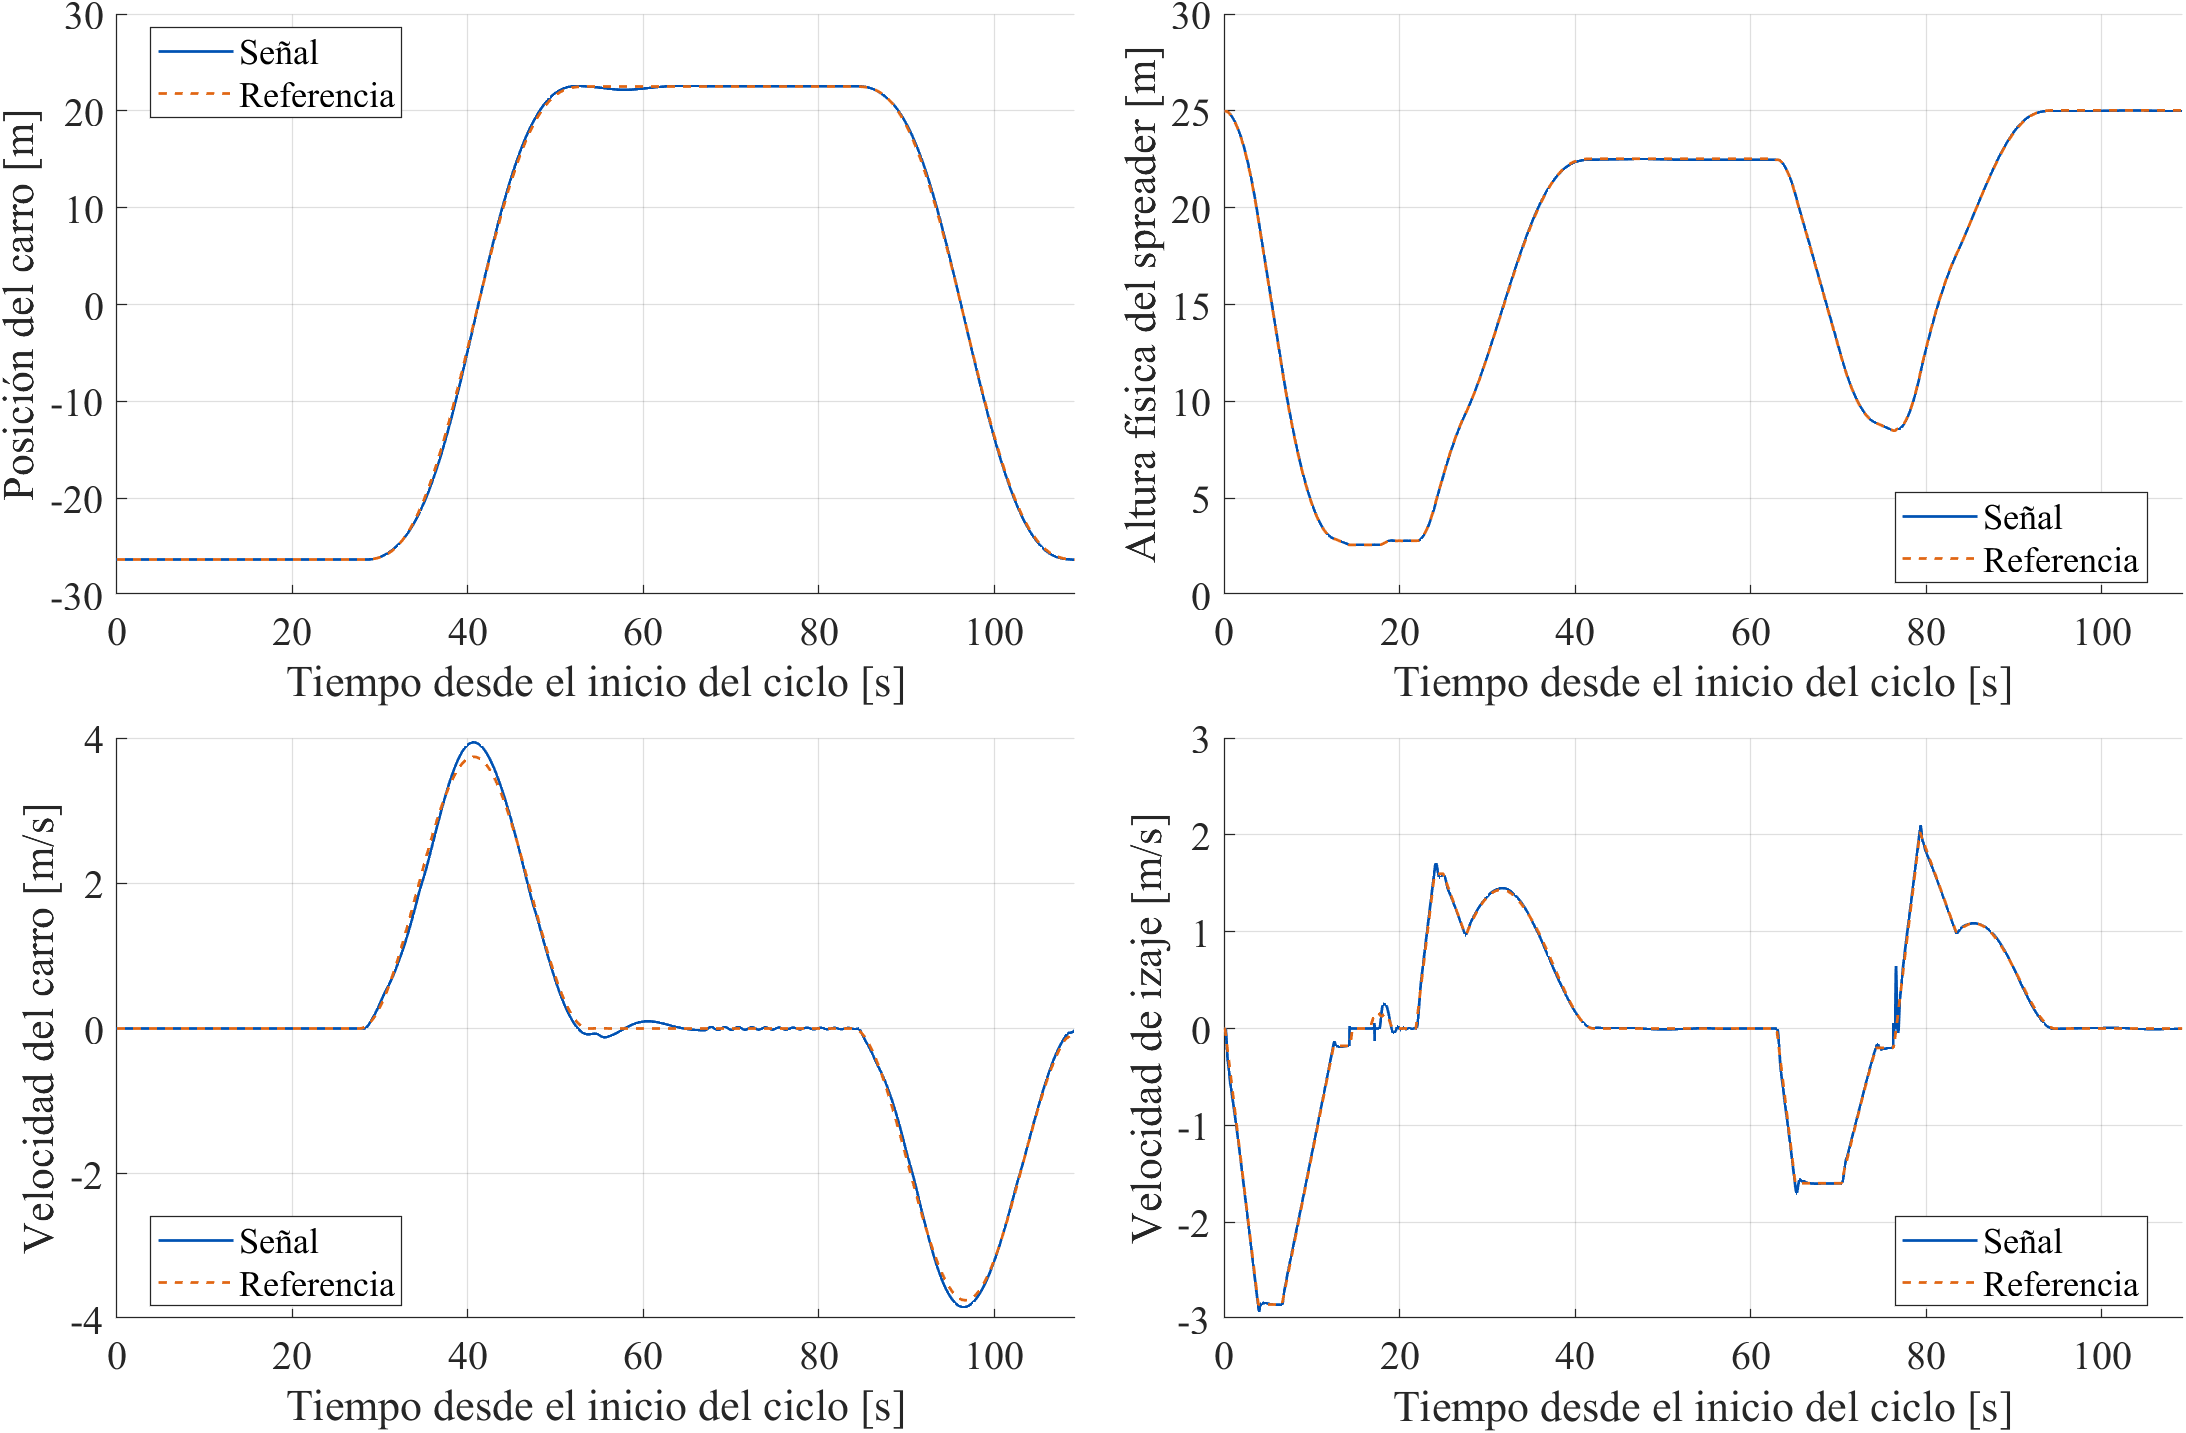
\includegraphics[width=.98\textwidth]{imagenes_informe/productividad/posicion_velocidad_ajustada.png}
\caption{Posición del carro, altura física del spreader y velocidades
frente a sus referencias durante el ciclo ajustado. La velocidad
de izaje corresponde al accionamiento. El tiempo se mide desde
el inicio del ciclo.}
\label{fig:productividad_seguimiento}
\end{figure}

La figura~\ref{fig:productividad_perfil} relaciona los traslados
automáticos con el perfil actualizado después de la toma y de la entrega.
La base cargada se obtiene descontando $H_c$ de la altura física;
en vacío se utiliza el plano inferior del spreader. El margen mínimo
sobre la línea de seguridad, evaluado bajo toda la huella durante AUTO,
fue $0{,}0417\un{m}$ con carga y $0{,}4816\un{m}$ en vacío.

\begin{figure}[H]\centering
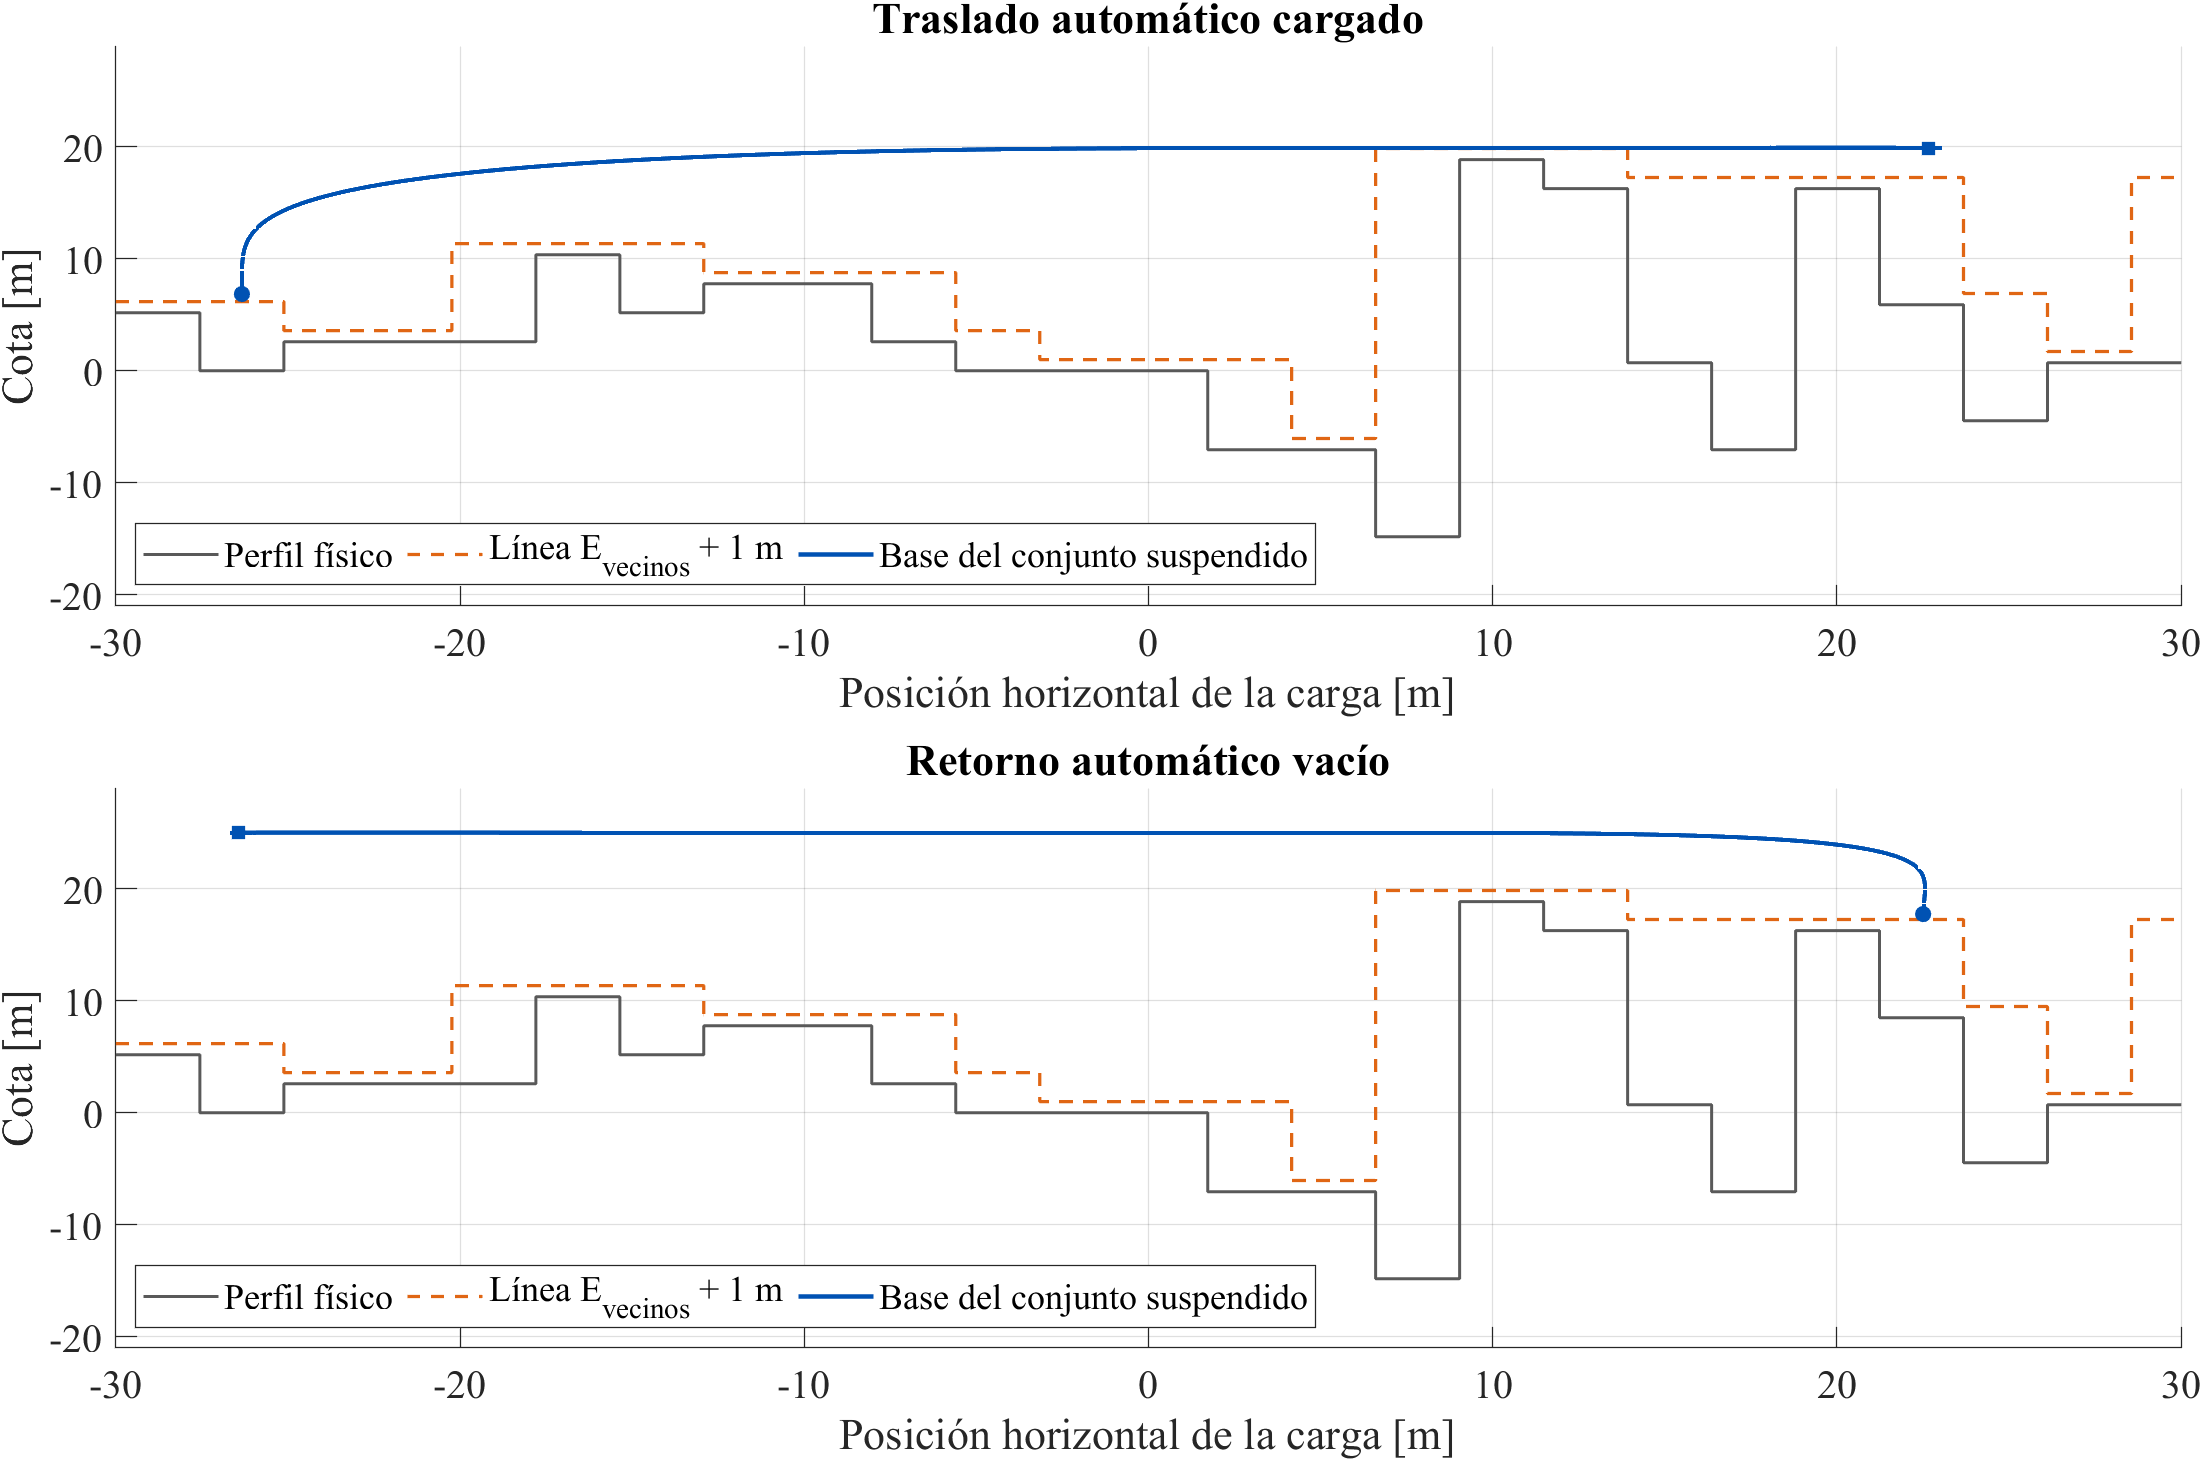
\includegraphics[width=.98\textwidth]{imagenes_informe/productividad/recorrido_perfil_ajustado.png}
\caption{Recorrido automático cargado y retorno vacío sobre el perfil
físico y la línea de seguridad local. El círculo indica el inicio
del intervalo y el cuadrado, su final.}
\label{fig:productividad_perfil}
\end{figure}

La figura~\ref{fig:productividad_balanceo} presenta el ángulo y la
velocidad angular sensados. Los umbrales dibujados corresponden
a la llegada y se verifican junto con posición y velocidad horizontal;
no representan límites de balanceo durante todo el transporte.

\begin{figure}[H]\centering
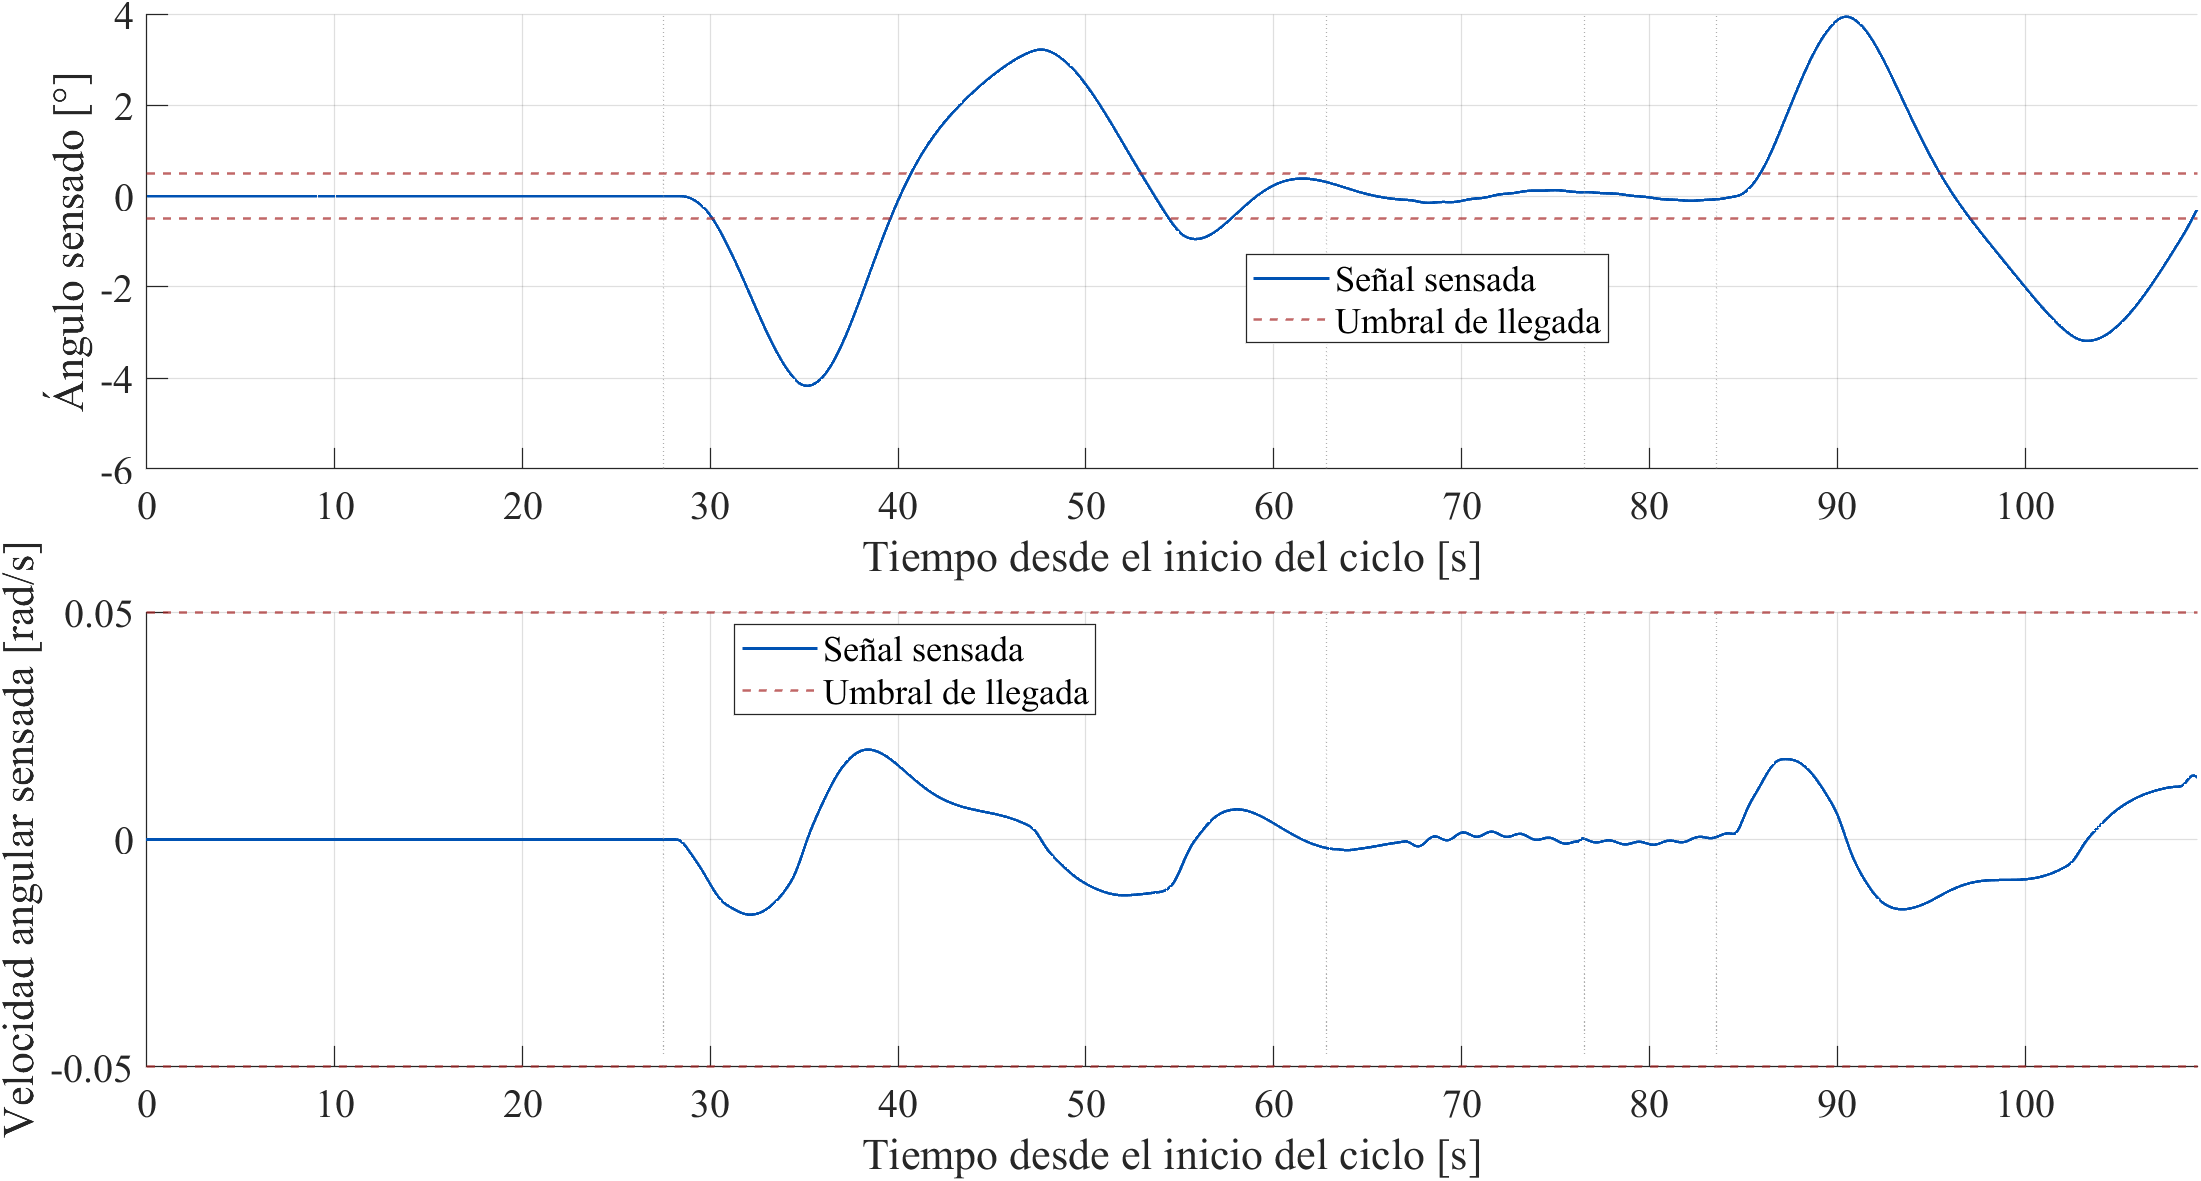
\includegraphics[width=.98\textwidth]{imagenes_informe/productividad/balanceo_ajustado.png}
\caption{Balanceo durante el ciclo ajustado. Las líneas verticales
señalan las solicitudes de AUTO cargado y MANUAL, la confirmación
de entrega y la solicitud de AUTO vacío. El tiempo se mide desde
el inicio del ciclo.}
\label{fig:productividad_balanceo}
\end{figure}

La tabla~\ref{tab:productividad_ajustada} resume las duraciones con
las mismas fronteras de etapa utilizadas en la evaluación inicial.
La reducción se distribuye entre las maniobras manuales y el transporte;
no se atribuye a una única ganancia.

\begin{table}[H]\centering\small
\caption{Duraciones del mismo ciclo antes y después del ajuste.}
\label{tab:productividad_ajustada}
\begin{tabularx}{\linewidth}{@{}Yrr@{}}\toprule
Etapa & Inicial [s] & Ajustado [s]\\\midrule
Descenso vacío hasta contacto & 37,72 & 14,32\\
Cierre de twistlocks & 1,04 & 1,04\\
Extracción, pesaje y solicitud de AUTO & 23,88 & 12,16\\
AUTO cargado hasta solicitud de MANUAL & 55,76 & 35,28\\
Cambio a MANUAL, descenso y entrega & 30,72 & 13,72\\
Extracción vacía y solicitud de AUTO & 22,00 & 7,04\\
AUTO vacío hasta condición de regreso & 46,52 & 25,36\\
Confirmación de reposo final & 0,28 & 0,24\\\midrule
\textbf{Ciclo completo} & \textbf{217,92} & \textbf{109,16}\\\bottomrule
\end{tabularx}
\end{table}

La productividad obtenida es
\begin{equation}
T_1=111{,}16-2{,}00=109{,}16\un{s},\qquad
P_1=\frac{3600}{109{,}16}=32{,}98\un{contenedores/h}.
\end{equation}
El ciclo queda $10{,}84\un{s}$ por debajo del objetivo de
$120\un{s}$. Frente al resultado inicial, el ahorro es de
$108{,}76\un{s}$, equivalente al $49{,}91\%$. Se cumple así
el requisito temporal para el recorrido y la masa ensayados.
La productividad media de otros recorridos y la operación con demoras
logísticas requieren una evaluación adicional.

\par
\Needspace{10\baselineskip}
\section{Conclusiones}

El trabajo permitió desarrollar e integrar un sistema de simulación y control jerárquico para una grúa portuaria STS, desde su modelado físico hasta la ejecución de maniobras semiautomáticas mediante autómatas implementados en CODESYS. La separación entre la regulación, ejecutada cada 1 ms, y la supervisión y la seguridad, con períodos de 20 ms, permitió coordinar los movimientos continuos con las secuencias operativas y evaluar el funcionamiento de la arquitectura en las etapas MIL y SIL.

Uno de los principales resultados de la integración fue identificar la influencia de la flexibilidad de la transmisión del carro, ausente en el modelo reducido utilizado para diseñar el regulador. La acumulación y posterior liberación de energía elástica podían provocar aceleraciones físicas superiores al límite del mando, aun cuando este permaneciera dentro de la banda establecida. La limitación de la variación de la anticipación angular del anti-sway, conservando la realimentación angular directa y el anti-windup, permitió reducir la aceleración física máxima de 1,454 a \(0{,}627\ \mathrm{m/s^2}\) y eliminar las excursiones fuera de la banda de \(\pm 0{,}8\ \mathrm{m/s^2}\) en la comparación controlada. También disminuyó la excitación mecánica durante la parada, con una reducción del 86,4\% en la energía elástica máxima y una incidencia mínima sobre la duración de la maniobra ensayada.

Los ensayos aislados confirmaron el seguimiento de perfiles suaves de izaje con carga y con el spreader vacío, sin cuerda floja ni saturación de torque durante el movimiento. En el carro, el anti-sway redujo el balanceo, aunque a costa de un mayor error de posición. Además, la sintonía más favorable durante el traslado no fue la mejor frente a una perturbación angular inicial. Estos resultados muestran que la selección de ganancias debe responder al compromiso operativo y verificarse bajo distintas condiciones de movimiento.

La planificación coordinada permitió ejecutar simultáneamente el izaje y la traslación, y adaptar la duración del movimiento horizontal cuando era necesario ganar altura para superar los obstáculos. La consideración de la envolvente local y la altura del contenedor vinculó las referencias con la geometría de la escena. Las pruebas completas en MIL y con la implementación manual en CODESYS realizaron el relevamiento y dos transferencias cargadas en sentidos opuestos, confirmando las tomas, las entregas y el balance de los perfiles de origen y destino. Desde START no se registraron emergencias ni fallas de seguimiento, y ambos accionamientos conservaron margen de torque. Estas corridas respaldan la integración funcional, aunque sus diferencias de duración no permiten comparar directamente la productividad.

La comparación del medio ciclo con y sin anti-sway mostró que la estabilización angular también condiciona la continuidad de la secuencia. En una ventana común posterior al traslado, la corrección redujo el ángulo RMS aproximadamente un 97,8\%. Sin ella, el carro alcanzó la zona horizontal de destino, pero el balanceo residual mantuvo inhibido el descenso y la prueba finalizó con la carga suspendida. Por lo tanto, el aporte del anti-sway no se limita a mejorar el movimiento, sino que permite alcanzar las condiciones necesarias para continuar la entrega.

La conversión de la regulación a un Motion Controller de dos ejes conservó el comportamiento de la implementación mediante bloques, con diferencias numéricas pequeñas en las variables comparadas y sin cambios en los tiempos de fase registrados. También reprodujo la mejora obtenida mediante la anticipación angular limitada. Por su parte, la migración de los autómatas a CODESYS permitió evaluar la programación manual en SFC y la generación automática en ST. Ambas mostraron comportamientos semejantes en el medio ciclo ensayado, aunque la extensión y complejidad del código autogenerado dificultaron su depuración.

La validación aislada de seguridad comprendió 25 escenarios y confirmó la retención de emergencias, el escalamiento ante fallas sucesivas y la vigilancia del watchdog. También permitió identificar aspectos que requieren revisión: la falta de intervención ante ciertos límites activos desde el arranque, la posible autorización del carro ante fallas simultáneas de ambos ejes y la necesidad de dos flancos de reinicio para recuperar el watchdog. Estas limitaciones delimitan el alcance de la validación obtenida y orientan las mejoras pendientes.

El cálculo sobre un ciclo que incluye la toma, el pesaje, la entrega
y el retorno vacío permitió identificar la limitación temporal de la configuración FF. La revisión conjunta de las maniobras, la planificación y la sintonía redujo el tiempo de $217{,}92$ a $109{,}16\un{s}$, una mejora del $49{,}91\%$, conservando la arquitectura regulatoria y ganancias constantes durante el frenado.
La productividad estimada de $32{,}98$ contenedores por hora satisface el objetivo en el ciclo evaluado.

En conjunto, los resultados respaldan la viabilidad funcional de la arquitectura bajo las condiciones de simulación evaluadas. El trabajo integra el modelo físico, la regulación y la supervisión secuencial en un banco que permite estudiar sus interacciones, y establece una base para corregir las limitaciones identificadas y ampliar la validación del sistema.

\par
\Needspace{10\baselineskip}
\section{Diccionario resumido de señales}
{\small
\renewcommand{\arraystretch}{1.10}
\begin{table}[H]
\centering
\caption{Señales principales del modelo.}
\begin{tabular}{L{4.3cm} L{2.4cm} L{7.0cm}}
\toprule
Señal & Unidad/tipo & Descripción\\
\midrule
$x_t$ & m & Posición horizontal del carro.\\
$v_t$ & m/s & Velocidad horizontal del carro.\\
$x_l,y_l$ & m & Posición del centro del cuerpo suspendido.\\
$l,l_h$ & m & Longitud geométrica y longitud comandada del cable.\\
$\theta_l$ & rad & Ángulo de balanceo respecto de la vertical.\\
$F_{hw}$ & N & Tensión equivalente por ramal.\\
$y_{c0}$ & m & Cota del perfil en la posición consultada.\\
\texttt{xRef}, \texttt{vxRef}, \texttt{axRef} & SI & Referencias del carro.\\
\texttt{yRef}, \texttt{vyRef}, \texttt{ayRef} & SI & Referencias del izaje.\\
\texttt{profileValid} & lógico & Perfil aceptado para su utilización; puede proceder del barrido validado o de la precarga del ensayo.\\
\texttt{profileScan}\newline\texttt{Complete} & lógico & Señala la finalización de la secuencia de barrido; no garantiza cobertura válida.\\
\texttt{loadedState} & lógico & Indica carga tomada desde DESPEGUE\_SUAVE; no implica pesaje completo.\\
\texttt{massEstimateValid} & lógico & Confirma que finalizó el pesaje.\\
\texttt{autoEntryHeightOK} & lógico & Perfil válido y altura medida suficiente según envolvente local.\\
\texttt{safetyEnvelope}\newline\texttt{Profile} & vector de 33 & Máximos locales del perfil y sus celdas vecinas.\\
\texttt{clearanceLineY} & m & Línea de seguridad calculada.\\
\texttt{swayControlEnable} & lógico & Habilitación efectiva de anti-sway.\\
\texttt{safetyPermitGlobal} & lógico & Permiso general del nivel 0.\\
\texttt{safetyPermitTrolley} & lógico & Permiso de movimiento horizontal.\\
\texttt{safetyPermitHoist} & lógico & Permiso de movimiento vertical.\\
\texttt{trackingFault} & lógico & Error de seguimiento sostenido.\\
\texttt{loadSequenceFault} & lógico & Falla de \textit{twistlocks} o secuencia de carga.\\
\texttt{watchdogToggle} & lógico & Pulso alternante del supervisor.\\
\bottomrule
\end{tabular}
\end{table}
}

\par
\Needspace{10\baselineskip}
\section{Índice compacto de funciones del supervisor}
\begin{table}[H]
\centering
\small
\caption{Funciones auxiliares implementadas dentro del supervisor.}
\begin{tabular}{L{5.2cm} L{8.5cm}}
\toprule
Función & Responsabilidad\\
\midrule
\texttt{procesarEntradasCrudas} & Detecta flancos, calcula aceleraciones, límites, torque comprobado y falla de seguimiento.\\
\texttt{registrarMuestraLidar} & Asigna una lectura al \textit{slot} y conserva la mayor cota.\\
\texttt{verificarCoberturaPerfil} & Comprueba que los 33 \textit{slots} tengan muestras.\\
\texttt{calcularVelocidadBarrido} & Genera velocidad limitada por distancia de frenado.\\
\texttt{calcularEnvolventeLocal} & Dilata el perfil mediante máximos de celdas vecinas.\\
\texttt{actualizarPerfilPorCarga} & Resta o suma una altura al tomar o liberar carga.\\
\texttt{calcularObjetivoSeguro} & Calcula altura local con carga, margen y estiramiento.\\
\texttt{retenerSolicitudHMI} & Memoriza la solicitud de barrido hasta atenderla o cancelarla.\\
\texttt{calcularFlagsSupervisor} & Calcula apoyo, intervención, reposo y proximidad al objetivo.\\
\texttt{calcularSuperficie}\newline\texttt{Objetivo} & Obtiene la mayor cota solapada por el contenedor.\\
\texttt{craneTrajectoryGenerator} & Planifica y evalúa los perfiles coordinados.\\
\texttt{cerrarLazoPosicionIzaje} & Corrige el error vertical final.\\
\texttt{referenciasManual} & Genera referencias manuales con rampas y saturaciones.\\
\texttt{referenciasBumpless} & Asegura continuidad durante los cambios de modo.\\
\texttt{referenciaDescensoFinal} & Mantiene el carro y permite descenso controlado.\\
\texttt{evaluarEstabilidad}\newline\texttt{Spreader} & Verifica ángulo y velocidad angular durante un tiempo.\\
\texttt{aplicarRetencionToma} & Inhibe movimientos hasta estabilizar después del cierre.\\
\texttt{detectarCuerdaFloja} & Aplica histéresis a la tensión del cable.\\
\texttt{calcularMandoManual} & Convierte \textit{joysticks} y aplica límites e interbloqueos.\\
\texttt{calcularDespeje} & Verifica línea de seguridad compensando estiramiento.\\
\texttt{calcularCodigos} & Codifica alarmas y fallas para el HMI.\\
\texttt{Estimar\_Masa} & Estima masa de contenedor a partir de la tensión.\\
\bottomrule
\end{tabular}
\end{table}

\par
\Needspace{10\baselineskip}
\section{Referencias}
\thispagestyle{mystyle}
{\small
\noindent [1] Universidad Nacional de Cuyo, Ingeniería Mecatrónica, ``317 -- Autómatas y Control Discreto. Proyecto Global Integrador 2025: Guía de trabajo Rev. 0 preliminar'', 2025.\par
\noindent [2] The MathWorks, Inc., \textit{Simulink User's Guide}, versión R2025b, 2025.\par
\noindent [3] The MathWorks, Inc., \textit{Stateflow User's Guide}, versión R2025b, 2025.\par
\noindent [4] K. Ogata, \textit{Ingeniería de control moderna}, 5.a ed. Pearson Educación, 2010.\par
\noindent [5] G. F. Franklin, J. D. Powell y A. Emami-Naeini, \textit{Feedback Control of Dynamic Systems}, 7.a ed. Pearson, 2015.\par
\noindent [6] W. Singhose, ``Command Shaping for Flexible Systems: A Review of the First 50 Years'', \textit{International Journal of Precision Engineering and Manufacturing}, vol. 10, n.º 4, pp. 153--168, 2009.\par

\noindent [7] SEW-EURODRIVE, \textit{MOVI-C CONTROLLER, documentación de sistema, edición 02/2026}. Consulta: 7 de octubre de 2026. \url{https://download.sew-eurodrive.com/download/html/33354448/en-EN/38976633995.html}.\par
\noindent [8] ABB, \textit{ACS880 position control}. Consulta: 7 de octubre de 2026. \url{https://www.abb.com/global/en/areas/motion/drives/expertise-technology/acs880-position-control}.\par
\noindent [9] Beckhoff Automation, \textit{AX8000: Product characteristics}. Consulta: 7 de octubre de 2026. \url{https://infosys.beckhoff.com/content/1033/ax8000_ba/7917947019.html}.\par
}


\par

\appendix
\clearpage
\section{Detalle del balance mecánico durante la parada manual}
\label{anexo:balance_mecanico}
Este anexo conserva el desglose concurrente de fuerzas y estados de la ley simple que complementa la comparación mecánica de la sección~\ref{sec:integracion_p1}.


La perturbación \textbf{sí aparece en el accionamiento}, pero antes del máximo del carro. Mirar solamente $a_{td}$ en $T_c$ ocultaría esa excitación inicial. En ese instante posterior se midieron simultáneamente:

\begin{equation}
a_t=-1,453512\ \mathrm{m/s^2},\qquad
a_{td}=-0,115336\ \mathrm{m/s^2},\qquad
a_{cmd}\simeq-0,78572\ \mathrm{m/s^2}.
\end{equation}

El esfuerzo de transmisión fue aproximadamente -41,141 kN, compuesto por \textbf{-41,121 kN elásticos} y \textbf{-20,797 N viscosos}. La fuerza pendular horizontal fue -2,467 kN y el rozamiento del carro aportó +3,254 N. El balance concurrente reproduce el pico:

\begin{equation}
a_t\simeq\frac{-41141,43-2467,18+3,25}{30000}
=-1,45351\ \mathrm{m/s^2}.
\end{equation}

La deformación concurrente fue -85,668 mm y la energía elástica 1761,4 J. El aporte elástico domina la fuerza de transmisión: la oscilación observada tiene una correspondencia cuantitativa con la deformación y energía del modelo, además de la evidencia obtenida al modificar la anticipación.


\begin{figure}[H]
\centering
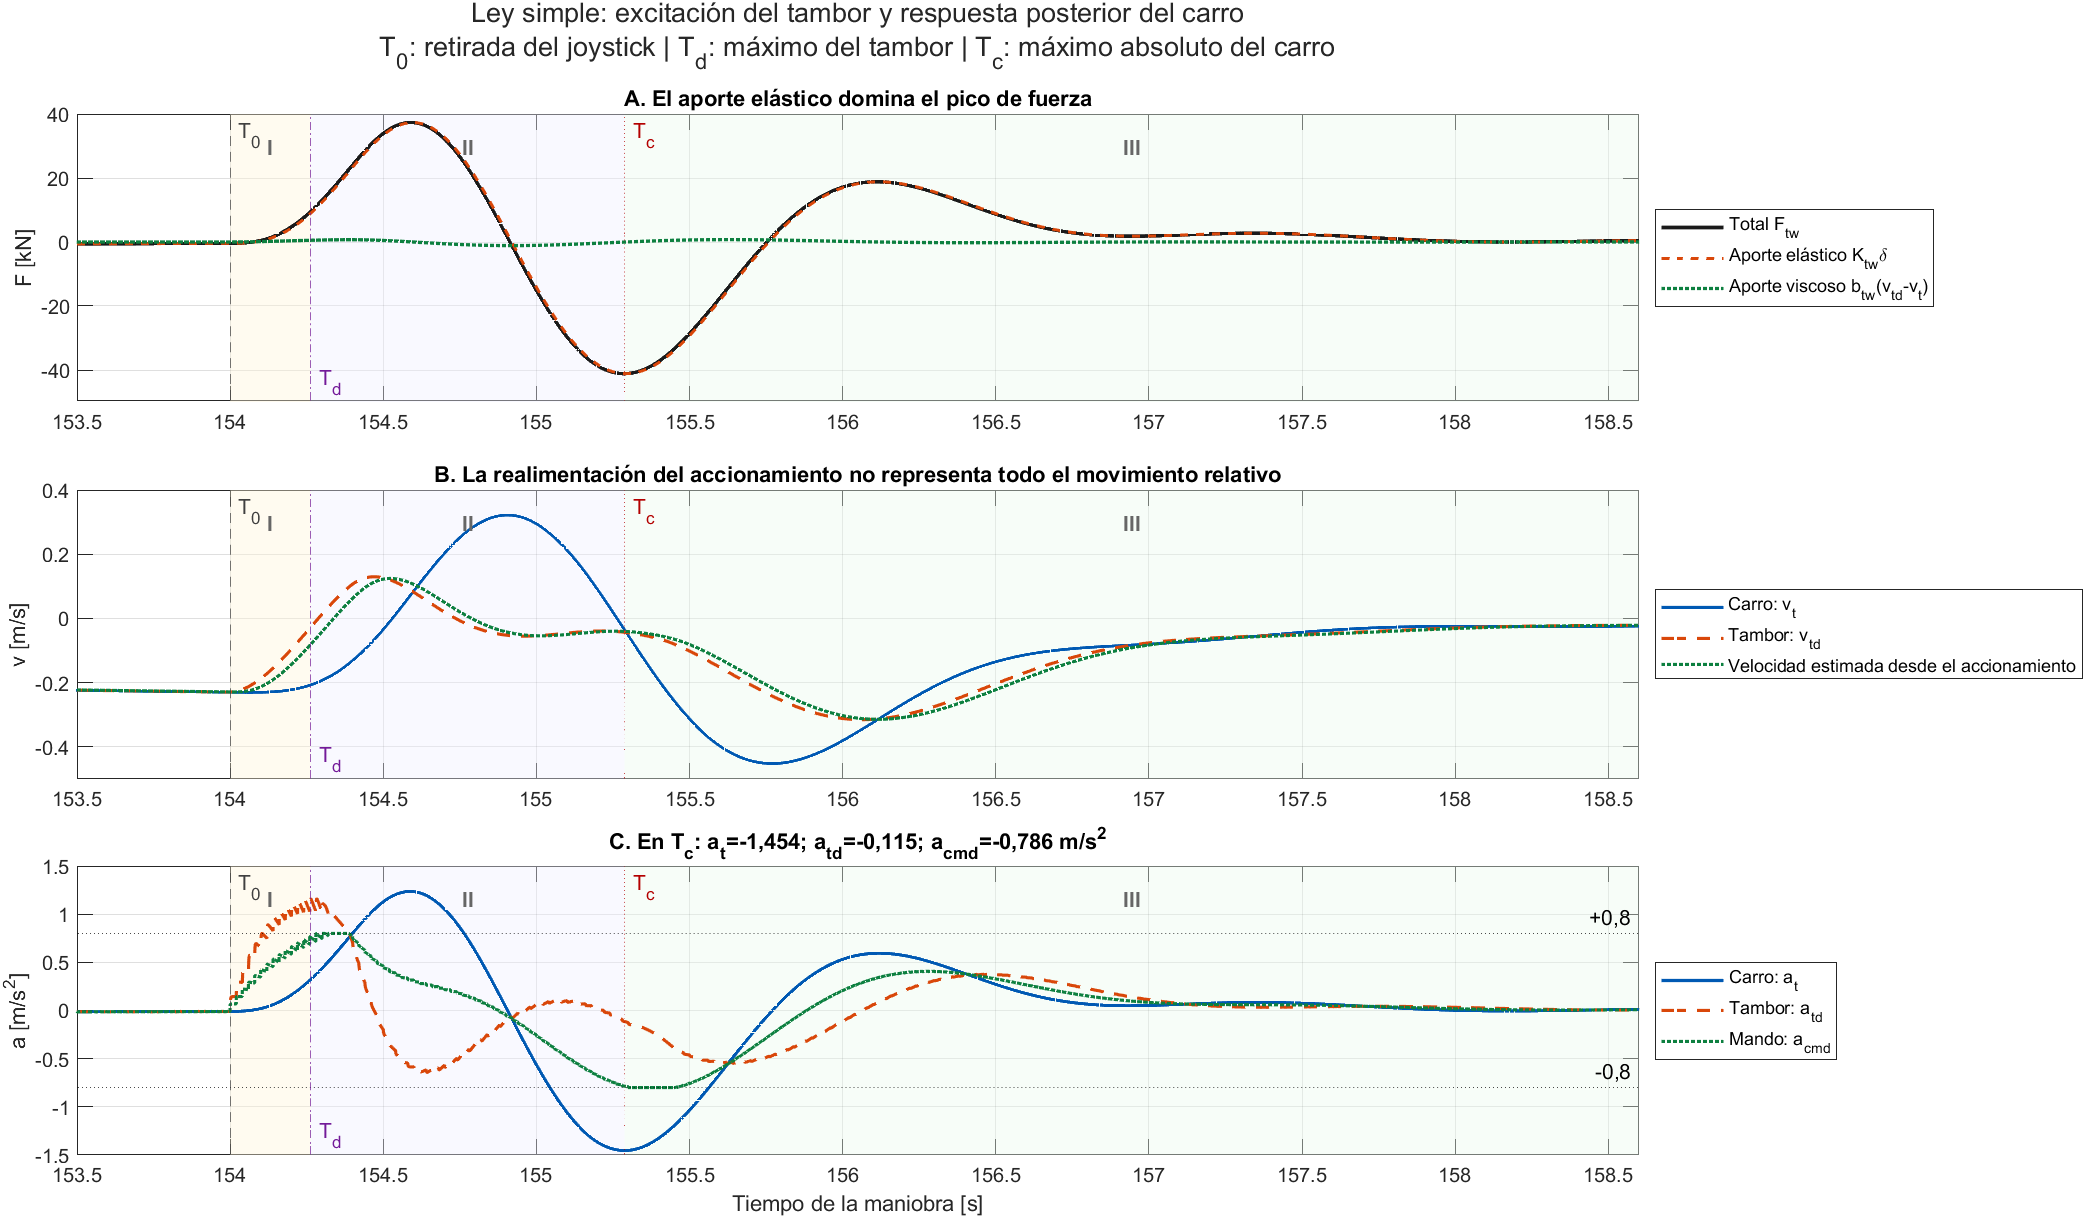
\includegraphics[width=0.99\textwidth,height=0.72\textheight,keepaspectratio]{imagenes_informe/usuario/integracionP1/05_04_balance_y_accionamiento.png}
\caption{Se muestra solamente la ley simple. A: fuerza total y aportes elástico y viscoso. B: velocidades físicas del carro y del tambor, junto con la velocidad estimada desde el accionamiento que recibe el controlador. C: aceleraciones del carro, del tambor y mando regulatorio. En esta figura los colores identifican magnitudes, no variantes; cada panel tiene su propia leyenda. Las referencias temporales y las zonas mantienen el significado de la \cref{fig:integracion_p1_4}.}
\label{fig:integracion_p1_5}
\end{figure}



\end{document}



